%% semifinal marks overfull lines with black rules; final is the copy for submission.
%% Build the final copy without editing this file:
%%   xelatex -jobname=sampleReport-final "\def\reportmode{final}%% semifinal marks overfull lines with black rules; final is the copy for submission.
%% Build the final copy without editing this file:
%%   xelatex -jobname=sampleReport-final "\def\reportmode{final}%% semifinal marks overfull lines with black rules; final is the copy for submission.
%% Build the final copy without editing this file:
%%   xelatex -jobname=sampleReport-final "\def\reportmode{final}%% semifinal marks overfull lines with black rules; final is the copy for submission.
%% Build the final copy without editing this file:
%%   xelatex -jobname=sampleReport-final "\def\reportmode{final}\input{sampleReport}"
\providecommand\reportmode{semifinal}
\documentclass[\reportmode]{cpecmu}

%% This is a sample document demonstrating how to use the CPECMU
%% project template. If you are having trouble, see "cpecmu.pdf" for
%% documentation.

\projectNo{S006-1}
\acadyear{2026}

%% ชื่อระบบ Collab Reflection เป็นชื่อรอง ใช้ \newline เพราะชื่อโครงงานถูกวางในเซลล์ตารางด้วย
\titleTH{แพลตฟอร์มประเมินตนเองและเพื่อนในกลุ่มเพื่อการพัฒนาตนเอง\newline Collab Reflection}
\titleEN{Self and Peer Evaluation Platform for Personal Development\newline Collab Reflection}

\author{นางสาวดารารัตน์ บัวยิ้ม}{Dararat Buayim}{660610759}
\author{นางสาวบัวชมพู ฤกษ์สุทธิรัตน์}{Buachompoo Rerksuitthirat}{660610768}
\author{นายปฏิพันธ์ เลขนอก}{Patiphan Leknok}{660610771}
\author{นายรัชชานนท์ ไชยวงค์}{Ratchanon Chaiwong}{660610789}

\cpeadvisor{thanatip}
%% ลำดับกรรมการตาม portal: สาลินี อานันท์ พฤษภ์
%% ชื่อภาษาอังกฤษยังไม่ได้ตรวจกับรายชื่อของภาค
\committee{ผศ.ดร.\,สาลินี สันติธีรากุล}{Asst.\,Prof.\,Salinee Santiteerakul, Ph.D.}
\cpecommittee{arnan}
\cpecommittee{pruet}

%% Some possible packages to include:
\usepackage[final]{graphicx} % for including graphics

%% Add bookmarks and hyperlinks in the document.
\PassOptionsToPackage{hyphens}{url}
\usepackage[colorlinks=true,allcolors=Blue4,citecolor=red,linktoc=all]{hyperref}
\def\UrlLeft#1\UrlRight{$#1$}

%% Needed just by this example, but maybe not by most reports
\usepackage{afterpage} % for outputting
\usepackage{pdflscape} % for landscape figures and tables. 
\usepackage{capt-of}   % caption for the plan (Gantt chart) table in chapter 1

%% Column types shared by the tables in chapters 2 and 3
\newcolumntype{Y}{>{\raggedright\arraybackslash}X}
\newcolumntype{P}[1]{>{\raggedright\arraybackslash}p{#1}}

%% Some other useful packages. Look these up to find out how to use
%% them.
% \usepackage{natbib}    % for author-year citation styles
% \usepackage{txfonts}
% \usepackage{appendix}  % for appendices on a per-chapter basis
% \usepackage{xtab}      % for tables that go over multiple pages
% \usepackage{subfigure} % for subfigures within a figure
% \usepackage{pstricks,pdftricks} % for access to special PostScript and PDF commands
% \usepackage{nomencl}   % if you have a list of abbreviations

%% if you're having problems with overfull boxes, you may need to increase
%% the tolerance to 9999
% \tolerance=9999
%% Thai text has few break points; allow extra stretch so lines do not run into the margin
\setlength{\emergencystretch}{2em}

\bibliographystyle{plain}
% \bibliographystyle{IEEEbib}

% \renewcommand{\topfraction}{0.85}
% \renewcommand{\textfraction}{0.1}
% \renewcommand{\floatpagefraction}{0.75}

%% Example for glossary entry
%% Need to use glossary option
%% See glossaries package for complete documentation.
\ifglossary
  \newglossaryentry{lorem ipsum}{
    name=lorem ipsum,
    description={derived from Latin dolorem ipsum, translated as ``pain itself''}
  }
\fi

%% Uncomment this command to preview only specified LaTeX file(s)
%% imported with \include command below.
%% Any other file imported via \include but not specified here will not
%% be previewed.
%% Useful if your report is large, as you might not want to build
%% the entire file when editing a certain part of your report.
% \includeonly{chapters/intro,chapters/background}

\begin{document}
\include{chapters/frontmatter}

\pagestyle{empty}\cleardoublepage
\normalspacing \setcounter{page}{1} \pagenumbering{arabic} \pagestyle{cpecmu}

\include{chapters/intro}
\include{chapters/background}
\include{chapters/approach}

\bibliography{sampleReport}

\ifproject
\normalspacing
\appendix
\include{chapters/appendix-interview}

%% Display glossary (optional) -- need glossary option.
\ifglossary\glossarypage\fi

%% Display index (optional) -- need idx option.
\ifindex\indexpage\fi

\fi % \ifproject
\end{document}
"
\providecommand\reportmode{semifinal}
\documentclass[\reportmode]{cpecmu}

%% This is a sample document demonstrating how to use the CPECMU
%% project template. If you are having trouble, see "cpecmu.pdf" for
%% documentation.

\projectNo{S006-1}
\acadyear{2026}

%% ชื่อระบบ Collab Reflection เป็นชื่อรอง ใช้ \newline เพราะชื่อโครงงานถูกวางในเซลล์ตารางด้วย
\titleTH{แพลตฟอร์มประเมินตนเองและเพื่อนในกลุ่มเพื่อการพัฒนาตนเอง\newline Collab Reflection}
\titleEN{Self and Peer Evaluation Platform for Personal Development\newline Collab Reflection}

\author{นางสาวดารารัตน์ บัวยิ้ม}{Dararat Buayim}{660610759}
\author{นางสาวบัวชมพู ฤกษ์สุทธิรัตน์}{Buachompoo Rerksuitthirat}{660610768}
\author{นายปฏิพันธ์ เลขนอก}{Patiphan Leknok}{660610771}
\author{นายรัชชานนท์ ไชยวงค์}{Ratchanon Chaiwong}{660610789}

\cpeadvisor{thanatip}
%% ลำดับกรรมการตาม portal: สาลินี อานันท์ พฤษภ์
%% ชื่อภาษาอังกฤษยังไม่ได้ตรวจกับรายชื่อของภาค
\committee{ผศ.ดร.\,สาลินี สันติธีรากุล}{Asst.\,Prof.\,Salinee Santiteerakul, Ph.D.}
\cpecommittee{arnan}
\cpecommittee{pruet}

%% Some possible packages to include:
\usepackage[final]{graphicx} % for including graphics

%% Add bookmarks and hyperlinks in the document.
\PassOptionsToPackage{hyphens}{url}
\usepackage[colorlinks=true,allcolors=Blue4,citecolor=red,linktoc=all]{hyperref}
\def\UrlLeft#1\UrlRight{$#1$}

%% Needed just by this example, but maybe not by most reports
\usepackage{afterpage} % for outputting
\usepackage{pdflscape} % for landscape figures and tables. 
\usepackage{capt-of}   % caption for the plan (Gantt chart) table in chapter 1

%% Column types shared by the tables in chapters 2 and 3
\newcolumntype{Y}{>{\raggedright\arraybackslash}X}
\newcolumntype{P}[1]{>{\raggedright\arraybackslash}p{#1}}

%% Some other useful packages. Look these up to find out how to use
%% them.
% \usepackage{natbib}    % for author-year citation styles
% \usepackage{txfonts}
% \usepackage{appendix}  % for appendices on a per-chapter basis
% \usepackage{xtab}      % for tables that go over multiple pages
% \usepackage{subfigure} % for subfigures within a figure
% \usepackage{pstricks,pdftricks} % for access to special PostScript and PDF commands
% \usepackage{nomencl}   % if you have a list of abbreviations

%% if you're having problems with overfull boxes, you may need to increase
%% the tolerance to 9999
% \tolerance=9999
%% Thai text has few break points; allow extra stretch so lines do not run into the margin
\setlength{\emergencystretch}{2em}

\bibliographystyle{plain}
% \bibliographystyle{IEEEbib}

% \renewcommand{\topfraction}{0.85}
% \renewcommand{\textfraction}{0.1}
% \renewcommand{\floatpagefraction}{0.75}

%% Example for glossary entry
%% Need to use glossary option
%% See glossaries package for complete documentation.
\ifglossary
  \newglossaryentry{lorem ipsum}{
    name=lorem ipsum,
    description={derived from Latin dolorem ipsum, translated as ``pain itself''}
  }
\fi

%% Uncomment this command to preview only specified LaTeX file(s)
%% imported with \include command below.
%% Any other file imported via \include but not specified here will not
%% be previewed.
%% Useful if your report is large, as you might not want to build
%% the entire file when editing a certain part of your report.
% \includeonly{chapters/intro,chapters/background}

\begin{document}
\maketitle
\makesignature

\ifproject
\begin{abstractTH}
Peer review คือการประเมินตนเองและประเมินเพื่อนในกลุ่ม ซึ่งเป็นกระบวนการสะท้อนคิดที่ช่วยให้ผู้เรียนเห็นจุดแข็งและจุดที่ควรพัฒนาของตนเอง ผ่านข้อเสนอแนะจากตนเอง เพื่อนร่วมกลุ่ม และอาจารย์ผู้สอน โดยการให้ข้อเสนอแนะเป็นกลไกสำคัญที่ผู้เรียนนำไปใช้พัฒนาการเรียนรู้และการทำงานร่วมกับผู้อื่นของตนเอง

ในปัจจุบัน การให้ข้อเสนอแนะในรายวิชาที่มีนักศึกษาจำนวนมากและมีการทำงานกลุ่มนั้นมีความยุ่งยาก เนื่องจากอาจารย์ผู้สอน (Instructor) ต้องอ่านผลประเมินทั้งหมด คัดแยกประเด็น และเขียนข้อเสนอแนะเฉพาะบุคคลให้นักศึกษาแต่ละคน ซึ่งเป็นภาระที่ใช้เวลามากและทำให้ไม่สามารถให้ข้อเสนอแนะได้อย่างทั่วถึง นอกจากนี้ ถ้อยคำในการประเมินเพื่อนบางครั้งอาจไม่เหมาะสม ทำให้ผู้รับข้อเสนอแนะไม่สามารถนำไปพัฒนาตนเองได้อย่างเต็มที่

คณะผู้จัดทำจึงได้จัดทำโครงงานเพื่อพัฒนาเว็บแอปพลิเคชัน Collab Reflection ที่ผสานเทคโนโลยีปัญญาประดิษฐ์ (AI) เข้า กับ Web Application ซึ่งสามารถให้นักศึกษาประเมินตนเองและประเมินเพื่อนในกลุ่มได้ และสามารถให้อาจารย์ดูผลการประเมินที่ถูกจำแนกประเภทผ่านแดชบอร์ดได้ โดยระบบในระยะที่ 1 ประกอบด้วย แบบประเมินตนเอง แบบประเมินเพื่อนในกลุ่ม และแดชบอร์ดสำหรับอาจารย์ ส่วนระยะที่ 2 จะเพิ่มระบบ AI ที่ช่วยตรวจโทนข้อความและเสนอถ้อยคำเชิงสร้างสรรค์ให้ผู้เขียนเลือกใช้ รวมถึง AI ที่สรุปผลเพื่อช่วยอาจารย์ร่างข้อเสนอแนะตอบกลับนักศึกษา โดยอาจารย์ยังเป็นผู้ตรวจทานก่อนส่งทุกครั้ง
\end{abstractTH}

\begin{abstract}
Peer review is a process of self-assessment and peer assessment within a group. It is a reflective practice that helps learners recognize their own strengths and areas for improvement through feedback from themselves, their teammates, and their instructors. Feedback serves as a key mechanism that learners use to improve their learning and their collaboration with others.

At present, providing feedback in courses with large numbers of students and group work is challenging. Instructors must read all of the evaluation results, categorize the issues, and write individualized feedback for each student. This is a time-consuming burden that prevents instructors from giving feedback to every student. In addition, the wording of peer evaluations is sometimes inappropriate, which prevents recipients from fully using the feedback to improve themselves.

Therefore, the project team developed Collab Reflection, a web application that integrates artificial intelligence (AI) technology with a web platform. The system allows students to evaluate themselves and their teammates, and allows instructors to view categorized evaluation results through a dashboard. Phase 1 of the system consists of a self-assessment form, a peer assessment form, and an instructor dashboard. Phase 2 will add an AI system that checks the tone of written comments and suggests constructive wording for the writer to choose from, as well as an AI that summarizes results to help instructors draft feedback responses to students. The instructor remains the reviewer before every message is sent.
\end{abstract}

\iffalse
\begin{dedication}
This document is dedicated to all Chiang Mai University students.

Dedication page is optional.
\end{dedication}
\fi % \iffalse

\begin{acknowledgments}
โครงงานแพลตฟอร์มประเมินตนเองและเพื่อนในกลุ่มเพื่อการพัฒนาตนเอง Collab Reflection สำเร็จลุล่วงไปได้ด้วยความกรุณาอย่างยิ่งจาก ผศ.ดร.ธนาทิพย์ จันทร์คง อาจารย์ที่ปรึกษา ที่ให้คำแนะนำ ข้อเสนอแนะ และการสนับสนุนทางวิชาการอย่างใกล้ชิดตลอดระยะเวลาการดำเนินโครงงาน รวมถึงชี้แนะแนวทางในการพัฒนาและปรับปรุงระบบให้มีประสิทธิภาพและเหมาะสมต่อการใช้งานจริง

ขอกราบขอบพระคุณ ผศ.ดร.พฤษภ์ บุญมา อ.ดร.อานันท์ สีห์พิทักษ์เกียรติ และ ผศ.ดร.สาลินี สันติธีรากุล คณะกรรมการสอบ ที่กรุณาให้คำแนะนำ ข้อคิดเห็น และข้อเสนอแนะอันเป็นประโยชน์ต่อโครงงาน

ขอขอบคุณภาควิชาวิศวกรรมคอมพิวเตอร์ คณะวิศวกรรมศาสตร์ มหาวิทยาลัยเชียงใหม่ ที่ให้ความรู้พื้นฐานทางวิชาการ ตลอดจนสนับสนุนทรัพยากร สถานที่ และอุปกรณ์ที่จำเป็นต่อการทำโครงงาน ทำให้คณะผู้จัดทำสามารถนำความรู้ที่ได้ศึกษามาประยุกต์ใช้พัฒนาระบบได้จริง

ขอขอบคุณเพื่อนร่วมทีมทุกคนที่ร่วมแรงร่วมใจกันในการออกแบบ พัฒนา และทดสอบระบบ ทั้งในช่วงที่งานดำเนินไปได้ด้วยดีและในช่วงที่พบอุปสรรค สมาชิกทุกคนช่วยเหลือ แลกเปลี่ยนความคิดเห็น และรับผิดชอบหน้าที่ของตนอย่างเต็มกำลัง จนโครงงานสำเร็จลุล่วงตามเป้าหมาย

ขอขอบคุณเพื่อนนักศึกษาและผู้ที่เกี่ยวข้อง ที่สละเวลาร่วมทดลองใช้งานระบบและให้ข้อเสนอแนะ ซึ่งเป็นประโยชน์ต่อการปรับปรุงระบบให้ตรงกับความต้องการของผู้ใช้มากยิ่งขึ้น

สุดท้ายนี้ ขอขอบคุณครอบครัวและผู้มีส่วนเกี่ยวข้องทุกท่าน ที่ให้การสนับสนุน กำลังใจ และความเข้าใจตลอดระยะเวลาการดำเนินโครงงาน คณะผู้จัดทำขอขอบพระคุณทุกท่านมา ณ โอกาสนี้

\acksign{2026}{10}{25}
\end{acknowledgments}%
\fi % \ifproject

\contentspage

\ifproject
\figurelistpage

\tablelistpage
\fi % \ifproject

% \abbrlist % this page is optional

% \symlist % this page is optional

% \preface % this section is optional


\pagestyle{empty}\cleardoublepage
\normalspacing \setcounter{page}{1} \pagenumbering{arabic} \pagestyle{cpecmu}

\chapter{\ifenglish Introduction\else บทนำ\fi}\label{ch:intro}

\section{\ifenglish Project rationale\else ที่มาและความสำคัญของโครงงาน\fi}

การเรียนรู้ในระดับอุดมศึกษาเกิดขึ้นภายในระบบนิเวศที่ประกอบด้วยผู้มีส่วนร่วมหลายฝ่าย ได้แก่ ผู้เรียน ซึ่งเป็นผู้สร้างความรู้และพัฒนาทักษะของตนเอง อาจารย์ ซึ่งเป็นผู้ออกแบบประสบการณ์การเรียนรู้และประเมินผล และเพื่อนร่วมชั้น ซึ่งเป็นทั้งผู้ร่วมงานและผู้สะท้อนพฤติกรรมการทำงานของกันและกัน สิ่งที่เชื่อมโยงทุกฝ่ายเข้าด้วยกันคือ ``กระบวนการการให้ข้อเสนอแนะ'' ซึ่งเป็นกลไกที่ทำให้ผู้เรียนรู้ว่าตนเองอยู่ตรงไหน ควรปรับปรุงอะไร และจะไปต่อทางใด

ข้อเสนอแนะที่มีคุณภาพไม่ได้จบที่การให้คะแนน แต่ต้องทำให้ผู้เรียนนำไปพัฒนาตนเองได้จริง กล่าวคือ ต้องเฉพาะเจาะจง ทันเวลา และเชื่อมโยงกับเป้าหมายการเรียนรู้ อย่างไรก็ตาม ในทางปฏิบัติ ข้อเสนอแนะลักษณะนี้ต้องอาศัยเวลาและแรงงานของอาจารย์เป็นอย่างมาก โดยเฉพาะในรายวิชาที่มีนักศึกษาจำนวนมาก (large-section courses) และมีการทำงานเป็นกลุ่ม อาจารย์มักไม่สามารถติดตามการมีส่วนร่วมของนักศึกษาแต่ละคนได้อย่างทั่วถึง ทำให้ข้อเสนอแนะที่นักศึกษาได้รับมีลักษณะกว้างและเหมือนกันทั้งกลุ่ม ไม่สะท้อนบทบาทและการพัฒนารายบุคคล นอกจากนี้การประเมินตนเองและประเมินเพื่อนมักทำเป็นครั้งคราว หรือทำเพียงเพื่อนำคะแนนไปคำนวณ จึงไม่เกิดการสะท้อนคิด (reflection) อย่างต่อเนื่อง ในด้านภาระงานของอาจารย์ ต้องอ่านผลประเมินและข้อความจำนวนมากด้วยตนเอง ทั้งเพื่อสรุปภาพรวม คัดแยกประเด็นที่ต้องติดตาม และเขียนข้อเสนอแนะตอบกลับ ซึ่งใช้เวลามากและทำได้ไม่ครบทุกคน ยิ่งไปกว่านั้น ในการประเมินเพื่อนอาจมีข้อความที่รุนแรง ไม่สร้างสรรค์ หรือเป็นการกล่าวโจมตีตัวบุคคล ซึ่งอาจส่งผลเสียต่อความสัมพันธ์ในกลุ่มและสุขภาวะของนักศึกษา แต่อาจารย์อาจตรวจพบไม่ทัน

ด้วยเหตุนี้เพื่อแก้ไขปัญหาดังกล่าว คณะผู้จัดทำจึงพัฒนา Collab Reflection แพลตฟอร์มที่ให้นักศึกษาประเมินตนเองและประเมินเพื่อนในกลุ่มอย่างเป็นระบบ โดยมุ่งเน้นให้ ``ข้อเสนอแนะเป็นเครื่องมือพัฒนาผู้เรียน'' อย่างเต็มรูปแบบ และใช้ปัญญาประดิษฐ์ (AI) เป็นผู้ช่วยลดภาระงานของอาจารย์ เพื่อให้อาจารย์เข้าถึงนักศึกษาจำนวนมากได้โดยไม่ลดคุณภาพของข้อเสนอแนะ ทั้งนี้ AI ทำหน้าที่เป็นผู้ช่วยเท่านั้น ไม่ได้แทนที่การตัดสินใจของอาจารย์ โดยอาจารย์ยังคงเป็นผู้ตรวจทานและเป็นผู้ให้ข้อเสนอแนะขั้นสุดท้ายแก่นักศึกษา

\section{\ifenglish Objectives\else วัตถุประสงค์ของโครงงาน\fi}

\begin{enumerate}
  \item เพื่อพัฒนาเว็บแอปพลิเคชัน Collab Reflection ที่ประกอบด้วยแบบประเมินตนเอง แบบประเมินเพื่อนในกลุ่ม และแดชบอร์ดสำหรับอาจารย์ผู้สอนที่แสดงและจำแนกประเภทผลการประเมิน
  \item เพื่อพัฒนาระบบ AI ที่ตรวจโทนข้อความในการประเมินเพื่อน และเสนอถ้อยคำเชิงสร้างสรรค์ให้ผู้เขียนเลือกใช้
  \item เพื่อพัฒนาระบบปัญญาประดิษฐ์ (AI) ที่สรุปผลการประเมิน เพื่อช่วยอาจารย์ร่างข้อเสนอแนะตอบกลับนักศึกษา โดยอาจารย์เป็นผู้ตรวจทานก่อนส่งทุกครั้ง
  \item เพื่อลดภาระของอาจารย์ในการให้ข้อเสนอแนะ และให้นักศึกษาได้รับข้อเสนอแนะที่เหมาะสมและทั่วถึง สำหรับนำไปพัฒนาการเรียนรู้และการทำงานร่วมกับผู้อื่น
\end{enumerate}

\section{\ifenglish Project scope\else ขอบเขตของโครงงาน\fi}

ผู้ใช้งาน : นักศึกษาและอาจารย์ผู้สอน

\subsection{ขอบเขตด้านฟังก์ชัน}

\begin{itemize}
  \item นักศึกษา
  \begin{enumerate}
    \item แบบประเมินตนเอง
    \item แบบประเมินเพื่อนในกลุ่ม
    \item ปัญญาประดิษฐ์ (AI) ตรวจโทนข้อความในการประเมินเพื่อน และเสนอถ้อยคำเชิงสร้างสรรค์ให้ผู้เขียนเลือกใช้
  \end{enumerate}
  \item อาจารย์ผู้สอน
  \begin{enumerate}
    \setcounter{enumii}{3}
    \item แดชบอร์ดสำหรับดูและจำแนกประเภทผลการประเมิน
    \item ปัญญาประดิษฐ์ (AI) สรุปผลการประเมินและช่วยร่างข้อเสนอแนะตอบกลับนักศึกษา โดยอาจารย์เป็นผู้ตรวจทานก่อนส่งทุกครั้ง
  \end{enumerate}
\end{itemize}

\subsection{ขอบเขตด้านการพัฒนา}

โครงงานแบ่งการพัฒนาเป็น 2 ระยะ ปัจจุบันเสร็จสิ้นการออกแบบระบบและการสาธิตต้นแบบ (demo) แล้ว และกำลังพัฒนาเว็บแอปพลิเคชันในระยะที่ 1 ซึ่งครอบคลุมแบบประเมินตนเอง แบบประเมินเพื่อนในกลุ่ม และแดชบอร์ดสำหรับอาจารย์ ส่วนระบบปัญญาประดิษฐ์ (AI) ทั้งสองส่วน (ตรวจโทนข้อความและสรุปผลร่างข้อเสนอแนะ) จะพัฒนาในระยะที่ 2

\subsection{ข้อจำกัดของขอบเขต}

\begin{itemize}
  \item ระยะที่ 1 ยังไม่รวมระบบปัญญาประดิษฐ์ (AI)
  \item ระบบยังไม่ได้ผสานกับระบบของมหาวิทยาลัย
  \item ในขั้นการออกแบบระบบและการสาธิตต้นแบบยังไม่ได้นำไปใช้งานในรายวิชาจริง
\end{itemize}

\section{\ifenglish Expected outcomes\else ประโยชน์ที่คาดว่าจะได้รับ\fi}

\begin{itemize}
  \item นักศึกษา
  \begin{itemize}
    \item ได้รับโอกาสสะท้อนคิดเกี่ยวกับการทำงานของตนเองและของกลุ่มอย่างสม่ำเสมอ
    \item ได้รับข้อเสนอแนะที่เฉพาะเจาะจงและเหมาะสมมากขึ้น ทำให้เห็นจุดแข็งและจุดที่ควรพัฒนาของตนเองได้ชัดเจน
    \item ได้ฝึกการให้ข้อเสนอแนะแก่เพื่อนด้วยถ้อยคำเชิงสร้างสรรค์ ซึ่งเป็นทักษะสำคัญในการทำงานร่วมกับผู้อื่น
  \end{itemize}
  \item อาจารย์ผู้สอน
  \begin{itemize}
    \item ประหยัดเวลาในการอ่านผลประเมิน คัดแยกประเด็น สรุปผล และเขียนข้อเสนอแนะ
    \item มองเห็นภาพรวมของผลการประเมินทั้งรายวิชาได้ง่ายผ่านแดชบอร์ด
    \item สามารถให้ความสำคัญกับนักศึกษาที่ต้องการความช่วยเหลือจริงได้ทันท่วงที
    \item ยังคงเป็นผู้ตรวจทานข้อเสนอแนะก่อนส่งทุกครั้ง จึงควบคุมคุณภาพของข้อเสนอแนะได้
  \end{itemize}
  \item รายวิชาและหน่วยงาน
  \begin{itemize}
    \item สามารถขยายการให้ข้อเสนอแนะเชิงพัฒนาไปยังนักศึกษาจำนวนมากได้อย่างทั่วถึง
    \item มีข้อมูลการประเมินที่เป็นระบบและจำแนกประเภทแล้ว สำหรับนำไปปรับปรุงการจัดกิจกรรมกลุ่มในรายวิชา
    \item เป็นแนวทางต้นแบบของการนำปัญญาประดิษฐ์ (AI) มาช่วยงานด้านการให้ข้อเสนอแนะในการเรียนการสอน โดยมีมนุษย์เป็นผู้ตัดสินใจขั้นสุดท้าย
  \end{itemize}
\end{itemize}

\section{\ifenglish Technology and tools\else เทคโนโลยีและเครื่องมือที่ใช้\fi}

\subsection{\ifenglish Hardware technology\else เทคโนโลยีด้านฮาร์ดแวร์\fi}

\begin{itemize}
  \item เครื่องคอมพิวเตอร์ส่วนบุคคลสำหรับพัฒนาระบบ
  \item เซิร์ฟเวอร์สำหรับติดตั้งและให้บริการระบบ
\end{itemize}

\subsection{\ifenglish Software technology\else เทคโนโลยีด้านซอฟต์แวร์\fi}

\begin{itemize}
  \item \textbf{React 19 (TypeScript) + Vite} -- พัฒนาส่วนหน้า (Frontend) ของเว็บแอปพลิเคชัน
  \item \textbf{Tailwind CSS} -- จัดรูปแบบและออกแบบหน้าตาของส่วนติดต่อผู้ใช้
  \item \textbf{TanStack Query และ Zustand} -- จัดการข้อมูลจากเซิร์ฟเวอร์และสถานะของแอปพลิเคชันฝั่งหน้าเว็บ
  \item \textbf{Node.js และ Express 5} -- พัฒนาส่วนหลังบ้าน (Backend) และ API
  \item \textbf{PostgreSQL และ Drizzle ORM} -- จัดเก็บข้อมูลการประเมิน และจัดการการเชื่อมต่อฐานข้อมูล
  \item \textbf{Qwen} -- โมเดลภาษา (LLM) สำหรับตรวจโทนข้อความ เสนอถ้อยคำเชิงสร้างสรรค์ และสรุปผลเพื่อช่วยอาจารย์ร่างข้อเสนอแนะ (ระยะที่ 2)
  \item \textbf{Docker และ nginx} -- จัดการสภาพแวดล้อมและติดตั้งระบบ (Deployment)
  \item \textbf{Vitest และ Cypress} -- ทดสอบระบบ (Unit Test และ End-to-End Test)
  \item \textbf{Git/GitHub และ Visual Studio Code} -- จัดการซอร์สโค้ดและพัฒนาโปรแกรม
\end{itemize}

\section{\ifenglish Project plan\else แผนการดำเนินงาน\fi}

แผนการดำเนินงานของโครงงานแสดงดังตารางที่~\ref{tab:ch1-plan} ณ วันที่จัดทำรายงานนี้ ขั้นตอนการค้นหางานวิจัยและกำหนดปัญหา การสัมภาษณ์อาจารย์ การออกแบบระบบและสร้างต้นแบบ (demo) รวมถึงการนำเสนอความก้าวหน้ารอบที่ 1 และ 2 ได้ดำเนินการเสร็จสิ้นแล้ว ส่วนการพัฒนาเว็บแอปพลิเคชันระยะที่ 1 อยู่ระหว่างดำเนินการ

% แผนภูมิแกนต์ใช้ environment plan ของ cpecmu.cls (\planitem{เดือนเริ่ม}{ปีเริ่ม ค.ศ.}{เดือนสิ้นสุด}{ปีสิ้นสุด}{ขั้นตอน})
% plan ไม่มีช่อง caption จึงใส่ด้วย \captionof (แพ็กเกจ capt-of ในไฟล์หลัก)
\captionof{table}{แผนการดำเนินงาน}\label{tab:ch1-plan}
\nopagebreak
\begin{plan}{7}{2026}{3}{2027}
    \planitem{7}{2026}{9}{2026}{ค้นหางานวิจัยและกำหนดปัญหา}
    \planitem{8}{2026}{8}{2026}{นำเสนอความก้าวหน้ารอบที่ 1}
    \planitem{9}{2026}{9}{2026}{สัมภาษณ์อาจารย์เพื่อรวบรวมความต้องการ}
    \planitem{8}{2026}{10}{2026}{ออกแบบระบบและสร้างต้นแบบ (demo)}
    \planitem{10}{2026}{10}{2026}{นำเสนอความก้าวหน้ารอบที่ 2}
    \planitem{11}{2026}{11}{2026}{รวบรวมความต้องการจากฝั่งนักศึกษา}
    \planitem{11}{2026}{12}{2026}{พัฒนาเว็บแอปพลิเคชันระยะที่ 1}
    \planitem{1}{2027}{2}{2027}{พัฒนาระบบปัญญาประดิษฐ์ (AI) (ระยะที่ 2)}
    \planitem{1}{2027}{2}{2027}{ทดสอบระบบ}
    \planitem{1}{2027}{3}{2027}{ทดลองใช้งานจริงกับรายวิชา}
    \planitem{2}{2027}{3}{2027}{ประเมินผลและสรุปผลการดำเนินงาน}
    \planitem{2}{2027}{3}{2027}{จัดทำรูปเล่มรายงาน}
\end{plan}

\section{\ifenglish Roles and responsibilities\else บทบาทและความรับผิดชอบ\fi}

คณะผู้จัดทำแบ่งบทบาทและหน้าที่ตามความถนัด ดังนี้

\begin{itemize}
  \item นายปฏิพันธ์ เลขนอก (Project Manager \& Backend) -- วางแผนและติดตามความคืบหน้าของโครงงาน ประสานงานระหว่างสมาชิกและอาจารย์ที่ปรึกษา พัฒนาส่วน Backend API และออกแบบฐานข้อมูล ใช้ความรู้ด้านการบริหารโครงการ Software Engineering และการออกแบบระบบฐานข้อมูล
  \item นางสาวดารารัตน์ บัวยิ้ม (Full-Stack \& Validation) -- พัฒนาส่วนหน้าเว็บของแบบประเมินและแดชบอร์ดอาจารย์ รวมถึงพัฒนา Backend API และเชื่อมต่อกับระบบปัญญาประดิษฐ์ (Qwen) ใช้ความรู้ด้าน Web Development, API Design และการประยุกต์ใช้โมเดลภาษา
  \item นายรัชชานนท์ ไชยวงค์ (Backend \& Tester) -- พัฒนาส่วน Backend และฐานข้อมูล วางแผนและดำเนินการทดสอบระบบทั้ง Unit Test และ End-to-End Test เพื่อตรวจสอบความถูกต้องของการทำงาน ใช้ความรู้ด้าน Software Testing, ฐานข้อมูล และการเขียน API
  \item นางสาวบัวชมพู ฤกษ์สุทธิรัตน์ (Frontend \& UX/UI) -- ออกแบบประสบการณ์และหน้าตาของผู้ใช้ (UX/UI) พัฒนาส่วนหน้าเว็บให้ใช้งานง่ายสำหรับนักศึกษาและอาจารย์ ใช้ความรู้ด้าน UX/UI Design, Frontend Development และการออกแบบส่วนติดต่อผู้ใช้
\end{itemize}

% บทที่ 2 เอกสารและงานวิจัยที่เกี่ยวข้อง
% ดึงจาก Google Doc ของทีม (Collab_Reflect_Report) เฉพาะบทที่ 2 เมื่อ 2026-11-05
% รายการอ้างอิงอยู่ใน sampleReport.bib
\chapter{\ifenglish Literature Review\else เอกสารและงานวิจัยที่เกี่ยวข้อง\fi}\label{ch:background}

โครงงาน Collab Reflection เป็นเว็บแอปพลิเคชันสำหรับสนับสนุนการสะท้อนคิดและการประเมินตนเองและเพื่อนร่วมทีม (Self- and Peer Assessment) โดยมุ่งเน้นการพัฒนาทักษะการทำงานเป็นทีมของนักศึกษาในรายวิชาที่มีผู้เรียนจำนวนมาก บทนี้นำเสนอแนวคิดและงานวิจัยที่ใช้เป็นพื้นฐานในการกำหนดแนวทางออกแบบระบบ ได้แก่ การเรียนรู้แบบร่วมมือ ปัญหาที่เกิดขึ้นในการทำงานกลุ่ม การประเมินโดยเพื่อนและการสะท้อนคิด เกณฑ์ประเมิน CATME แนวทางจัดการข้อเสนอแนะที่อ่อนไหว การคุ้มครองข้อมูลส่วนบุคคล ตลอดจนเทคโนโลยีและสถาปัตยกรรมที่เกี่ยวข้องกับการพัฒนาระบบ

\section{การทำงานเป็นทีมและการเรียนรู้แบบร่วมมือ}

การเรียนรู้แบบร่วมมือ (Cooperative Learning) เป็นการจัดการเรียนรู้ที่ให้ผู้เรียนทำงานร่วมกันเป็นกลุ่มขนาดเล็กเพื่อบรรลุเป้าหมายร่วมกัน สมาชิกแต่ละคนต้องพึ่งพาและสนับสนุนกัน โดยมีองค์ประกอบสำคัญ ได้แก่ การพึ่งพากันในเชิงบวก (positive interdependence) ความรับผิดชอบรายบุคคล (individual accountability) การปฏิสัมพันธ์ระหว่างสมาชิก ทักษะทางสังคม และการประมวลผลกระบวนการกลุ่ม (group processing)~\cite{johnson1998active} องค์ประกอบเหล่านี้ชี้ให้เห็นว่าความสำเร็จของการทำงานกลุ่มไม่ได้พิจารณาจากผลงานสุดท้ายเพียงอย่างเดียว แต่ควรพิจารณาพฤติกรรมและการมีส่วนร่วมของสมาชิกแต่ละคนด้วย

สำหรับรายวิชาที่มีการทำงานกลุ่ม ผู้สอนอาจเห็นผลงานที่ส่งได้ชัดเจนกว่ากระบวนการทำงานระหว่างสมาชิก โดยเฉพาะกิจกรรมที่เกิดขึ้นนอกชั้นเรียน การมีเครื่องมือให้สมาชิกประเมินตนเองและสะท้อนพฤติกรรมของเพื่อนจึงช่วยเพิ่มข้อมูลประกอบการติดตามการทำงานเป็นทีม ซึ่งเป็นแนวคิดหลักของ Collab Reflection

\subsection{ขั้นตอนพัฒนาการของกลุ่ม}

Tuckman เสนอว่ากลุ่มมักพัฒนาผ่าน 4 ขั้นตอน ได้แก่ Forming (การเริ่มรวมกลุ่ม) Storming (การเผชิญความเห็นต่าง) Norming (การสร้างบรรทัดฐานร่วมกัน) และ Performing (การทำงานเพื่อบรรลุเป้าหมาย)~\cite{tuckman1965developmental} ในช่วงเริ่มต้น สมาชิกอาจยังไม่เข้าใจบทบาทและความคาดหวังของกันและกัน ส่วนช่วง Storming อาจเกิดความขัดแย้งเกี่ยวกับหน้าที่ วิธีทำงาน หรือการสื่อสาร การกำหนดข้อตกลงกลุ่มและทบทวนการทำงานเป็นระยะจึงเป็นแนวทางช่วยให้สมาชิกเข้าใจความรับผิดชอบร่วมกัน

แนวคิดดังกล่าวสอดคล้องกับฟีเจอร์ข้อตกลงกลุ่มของ Collab Reflection ซึ่งเปิดให้อาจารย์นำเอกสารข้อตกลงมาให้สมาชิกศึกษา และใช้การประเมินหลายรอบเพื่อสนับสนุนการสะท้อนพฤติกรรมระหว่างภาคการศึกษา ทั้งนี้ ระบบเป็นเครื่องมือช่วยติดตามและสื่อสาร ไม่ได้ทำหน้าที่แก้ไขความขัดแย้งแทนการพูดคุยระหว่างสมาชิก

\section{ปัญหาที่พบในการทำงานกลุ่ม}

\subsection{Social Loafing และ Free-rider}

Social Loafing หมายถึงปรากฏการณ์ที่บุคคลมีแนวโน้มใช้ความพยายามน้อยลงเมื่อทำงานเป็นกลุ่ม เมื่อเทียบกับการทำงานคนเดียว~\cite{latane1979many} หากสมาชิกทุกคนได้รับคะแนนจากผลงานกลุ่มเท่ากัน อาจเกิดสถานการณ์ที่สมาชิกบางคนมีส่วนร่วมน้อยแต่ได้รับผลลัพธ์เท่ากับสมาชิกที่ทำงานมากกว่า ซึ่งมักเรียกว่า Free-rider ขณะเดียวกันสมาชิกที่รับผิดชอบงานมากอาจต้องแบกรับภาระของกลุ่ม

ประเด็นนี้สอดคล้องกับผลการสัมภาษณ์อาจารย์ผู้สอน 5 ท่านในโครงงาน ซึ่งพบปัญหาสมาชิกไม่ช่วยงานและสมาชิกบางคนต้องรับภาระงานแทนผู้อื่น ดังนั้น Collab Reflection จึงให้สมาชิกประเมินพฤติกรรมการทำงานของตนเองและเพื่อนตามเกณฑ์เดียวกัน พร้อมแสดงผลรายด้านให้อาจารย์ใช้ประกอบการติดตาม โดยผลการประเมินไม่ควรถูกใช้เป็นข้อสรุปเกี่ยวกับบุคคลโดยปราศจากการพิจารณาบริบทอื่น

\subsection{ข้อจำกัดด้านอัตราส่วนผู้สอนต่อนักศึกษา}

ในรายวิชาที่มีนักศึกษาจำนวนมาก ผู้สอนอาจไม่สามารถสังเกตพฤติกรรมการทำงานของสมาชิกทุกคนได้อย่างทั่วถึง โดยเฉพาะการแบ่งงาน การสื่อสาร และการช่วยเหลือกันนอกชั้นเรียน ข้อมูลจากการสัมภาษณ์ในโครงงานสะท้อนว่าผู้สอนต้องการเครื่องมือที่เรียบง่าย ลดภาระการติดตาม และช่วยให้มองเห็นปัญหาของแต่ละทีมได้รวดเร็วขึ้น

Collab Reflection จึงออกแบบแดชบอร์ดสำหรับแสดงภาพรวมผลประเมิน ติดตามจำนวนผู้ส่ง และแจ้งสัญญาณจากรูปแบบคะแนน เช่น คะแนนเฉลี่ยที่ต่ำในบางด้านหรือความแตกต่างระหว่างคะแนนประเมินตนเองกับคะแนนจากเพื่อน สัญญาณดังกล่าวเป็นข้อมูลเพื่อช่วยจัดลำดับการติดตาม ไม่ใช่การวินิจฉัยหรือการตัดสินนักศึกษาโดยอัตโนมัติ

\section{การประเมินโดยเพื่อนร่วมกลุ่มและการประเมินตนเอง}

การประเมินโดยเพื่อน (Peer Assessment) เป็นกระบวนการที่ผู้เรียนพิจารณาคุณภาพหรือพฤติกรรมของเพื่อนในระดับเดียวกัน โดยอาศัยเกณฑ์หรือเป้าหมายที่กำหนดไว้ ส่วนการประเมินตนเอง (Self-assessment) เปิดโอกาสให้ผู้เรียนทบทวนผลงานและพฤติกรรมของตนเอง การใช้ทั้งสองวิธีร่วมกันช่วยให้ผู้เรียนได้รับมุมมองที่หลากหลายและมีส่วนรับผิดชอบต่อการเรียนรู้ของตนเอง~\cite{topping1998peer}

ในบริบทของโครงงานนี้ การประเมินเพื่อนไม่ได้มุ่งเป็นเครื่องมือตัดเกรดเพียงอย่างเดียว แต่เป็นพื้นที่สะท้อนพฤติกรรมและการมีส่วนร่วมของสมาชิก โดยเน้นข้อเสนอแนะเชิงสร้างสรรค์ (Constructive Feedback) ที่ผู้รับสามารถนำไปปรับปรุงการทำงานในรอบถัดไปได้ อย่างไรก็ตาม การประเมินอาจได้รับอิทธิพลจากความสนิทสนม ความเกรงใจ หรือความขัดแย้งส่วนบุคคล ระบบจึงออกแบบให้ปกปิดตัวตนผู้ประเมิน ใช้ข้อมูลจากหลายมุมมอง และให้อาจารย์เป็นผู้ตรวจทานก่อนเผยแพร่ผล

\subsection{การประเมินระหว่างทางและการประเมินเพื่อสรุปผล}\label{sec:ch2-formative}

การประเมินระหว่างทาง (Formative Assessment) มีเป้าหมายเพื่อให้ข้อเสนอแนะระหว่างกระบวนการเรียนรู้ เพื่อนำไปปรับปรุงการทำงาน ส่วนการประเมินเพื่อสรุปผล (Summative Assessment) ใช้พิจารณาผลสัมฤทธิ์เมื่อสิ้นสุดช่วงการเรียนรู้~\cite{black1998assessment} แนวคิดนี้เป็นพื้นฐานของการกำหนดประเภทรอบประเมินใน Collab Reflection โดยอาจารย์สามารถกำหนดรอบฝึกเพื่อการพัฒนา และรอบเก็บคะแนนตามวัตถุประสงค์ของรายวิชาได้

\subsection{ระบบประเมินโดยเพื่อนที่เกี่ยวข้อง}

ระบบที่มีอยู่เดิมเป็นแนวทางอ้างอิงในการกำหนดความสามารถของ Collab Reflection โดยแต่ละระบบมีจุดเน้นแตกต่างกัน ดังตารางที่~\ref{tab:ch2-1}

\begin{table}[htbp]
\centering
\caption{การเปรียบเทียบระบบประเมินโดยเพื่อนร่วมกลุ่มที่เกี่ยวข้อง}\label{tab:ch2-1}
\begin{tabularx}{\textwidth}{P{0.2\textwidth}YY}
\hline
\textbf{ระบบ} & \textbf{ลักษณะการทำงานตามเอกสารที่ศึกษา} & \textbf{ประเด็นที่นำมาใช้เป็นแนวทาง} \\ \hline
CATME Peer Evaluation & ประเมินสมาชิกในทีมตามพฤติกรรมหลายด้าน รองรับการประเมินตนเอง การประเมินเพื่อน และความคิดเห็นเป็นข้อความ~\cite{ohland2012catme} & ใช้กรอบพฤติกรรม 5 ด้านเป็นพื้นฐานของเกณฑ์ประเมิน \\
FeedbackFruits Peer Review & รองรับการประเมินผลงานตามเกณฑ์และ Rubric การรีวิวแบบไม่เปิดเผยตัวตน และมี AI Feedback Coach & ใช้เป็นตัวอย่างการผสานเกณฑ์ประเมินกับเครื่องมือสนับสนุนการให้ข้อเสนอแนะ \\
Peerceptiv Peer Assessment & รองรับการให้คะแนนและเขียนความคิดเห็นเกี่ยวกับผลงาน รวมถึงการประเมินการมีส่วนร่วม การสื่อสาร และการทำงานร่วมกัน ตลอดจนการรีวิวแบบไม่เปิดเผยตัวตน & ใช้เป็นตัวอย่างระบบที่รวบรวมการประเมินจากผู้เรียนหลายคน \\ \hline
\end{tabularx}
\end{table}

จากแนวทางข้างต้น Collab Reflection มุ่งรวมการประเมินตนเอง การประเมินเพื่อนในทีม เกณฑ์ที่อธิบายพฤติกรรม การสะท้อนคิดแบบคำถามปลายเปิด และแดชบอร์ดสำหรับอาจารย์ไว้ในแพลตฟอร์มเดียว ส่วนการใช้ปัญญาประดิษฐ์ (AI) เพื่อช่วยตรวจโทนข้อความและสรุปความคิดเห็นถูกกำหนดเป็นฟีเจอร์ในระยะที่ 2 ตามแผนการพัฒนาของระบบ

\section{การสะท้อนคิดและการให้ข้อเสนอแนะ}

การสะท้อนคิด (Reflection) เป็นกระบวนการทบทวนประสบการณ์เพื่อสร้างความเข้าใจและนำสิ่งที่เรียนรู้ไปปรับใช้ในการปฏิบัติครั้งต่อไป Kolb อธิบายวงจรการเรียนรู้จากประสบการณ์ไว้ 4 ขั้น ได้แก่ ประสบการณ์รูปธรรม การสังเกตและสะท้อนคิด การสร้างแนวคิดนามธรรม และการทดลองปฏิบัติ~\cite{kolb1984experiential} ส่วน Schön แบ่งการสะท้อนคิดเป็นการสะท้อนคิดขณะปฏิบัติ (Reflection-in-action) และการสะท้อนคิดหลังปฏิบัติ (Reflection-on-action)~\cite{schon1983reflective}

Collab Reflection เน้นการสะท้อนคิดหลังปฏิบัติ โดยให้นักศึกษาทบทวนการทำงานของตนเองและเพื่อนเป็นรอบตามช่วงเวลาที่อาจารย์กำหนด คำถามปลายเปิดใช้แนวคิด ``ให้ดอกไม้ เติมปุ๋ย'' โดย ``ดอกไม้'' ให้ระบุสิ่งที่สมาชิกทำได้ดี ส่วน ``ปุ๋ย'' ให้เสนอสิ่งที่ช่วยให้สมาชิกทำได้ดีขึ้นในงานถัดไป สำหรับการประเมินตนเองจะปรับเป็นการระบุสิ่งที่ตนทำได้ดีและสิ่งที่ต้องการปรับปรุง

Hattie และ Timperley อธิบายว่าข้อเสนอแนะที่มีประสิทธิภาพควรช่วยให้ผู้เรียนเข้าใจเป้าหมาย ความก้าวหน้าในปัจจุบัน และแนวทางดำเนินการต่อไป~\cite{hattie2007feedback} ดังนั้นระบบจึงแนะนำให้ผู้ประเมินกล่าวถึงพฤติกรรมหรือผลงานที่สังเกตได้จริง และเสนอแนวทางที่นำไปปฏิบัติได้ แทนการตำหนิหรือตัดสินตัวบุคคล

\section{เกณฑ์การประเมินแบบ CATME}

โครงงานเลือกใช้กรอบการประเมินสมาชิกทีมของ CATME (Comprehensive Assessment of Team Member Effectiveness) เป็นพื้นฐาน โดย CATME พัฒนาเกณฑ์แบบมาตราส่วนที่มีคำอธิบายพฤติกรรมกำกับ (Behaviorally Anchored Rating Scale: BARS) สำหรับการประเมินตนเองและเพื่อน~\cite{ohland2012catme} กรอบดังกล่าวแบ่งพฤติกรรมการทำงานเป็นทีมออกเป็น 5 ด้าน ดังตารางที่~\ref{tab:ch2-2}

\begin{table}[htbp]
\centering
\caption{องค์ประกอบการประเมินพฤติกรรมการทำงานเป็นทีมตามแนวคิด CATME}\label{tab:ch2-2}
\begin{tabularx}{\textwidth}{P{0.32\textwidth}Yl}
\hline
\textbf{ด้านการประเมิน} & \textbf{พฤติกรรมที่พิจารณา} & \textbf{กลุ่มด้าน} \\ \hline
การมีส่วนร่วมในงาน (Contributing to the Team's Work) & ทำงานที่ได้รับมอบหมายให้ครบถ้วนและตรงเวลา รวมถึงช่วยเหลือเพื่อนเมื่อจำเป็น & ด้านงาน \\
การปฏิสัมพันธ์กับเพื่อน (Interacting with Teammates) & รับฟังความคิดเห็น สื่อสารอย่างชัดเจน และปฏิบัติต่อสมาชิกอย่างเหมาะสม & ด้านทีม \\
การดูแลให้ทีมดำเนินตามแผน (Keeping the Team on Track) & ติดตามความคืบหน้า ประสานงาน และช่วยให้ทีมดำเนินงานตามแผน & ด้านทีม \\
การคาดหวังคุณภาพ (Expecting Quality) & ใส่ใจคุณภาพของงานและสนับสนุนให้ผลงานของทีมมีคุณภาพ & ด้านงาน \\
ความรู้และทักษะที่เกี่ยวข้อง (Having Relevant KSAs) & มีความรู้ ทักษะ และความสามารถที่จำเป็นต่อการทำงานของทีม & ด้านงาน \\ \hline
\end{tabularx}
\end{table}

ในระบบกำหนดคะแนนระดับ 1--5 โดยมีคำอธิบายพฤติกรรมที่ระดับ 1, 3 และ 5 ส่วนระดับ 2 และ 4 เป็นค่าระหว่างกลาง เพื่อให้ผู้ประเมินใช้พฤติกรรมที่สังเกตได้เป็นหลักในการเลือกคะแนน ตัวอย่างเช่น ระดับ 1 หมายถึงพฤติกรรมต่ำกว่าที่คาดหวัง ระดับ 3 หมายถึงทำได้ตามที่คาดหวัง และระดับ 5 หมายถึงทำได้เกินกว่าที่คาดหวัง

นอกจากคะแนนทั้ง 5 ด้านแล้ว แบบประเมินยังมีคำถามปลายเปิดเพื่อระบุจุดแข็งและสิ่งที่ควรพัฒนา ระบบคำนวณค่าเฉลี่ยคะแนนที่เพื่อนให้ในแต่ละด้านโดยไม่รวมคะแนนประเมินตนเอง แล้วนำมาเปรียบเทียบกับคะแนนที่นักศึกษาประเมินตนเอง เพื่อให้เห็นความแตกต่างระหว่างมุมมอง ทั้งนี้การเปรียบเทียบมีไว้เพื่อการสะท้อนคิด ไม่ใช่ข้อสรุปว่ามุมมองใดถูกต้องกว่า

การคำนวณคะแนนถ่วงน้ำหนักร่วมกับคะแนนชิ้นงานเป็นฟีเจอร์ที่วางแผนไว้ในระยะที่ 3 ตามการออกแบบในบทที่~\ref{ch:method} จึงไม่ถือเป็นความสามารถของระบบในระยะที่ 1

\section{การจัดการข้อเสนอแนะที่อ่อนไหวและการคุ้มครองข้อมูลส่วนบุคคล}

การประเมินเพื่อนเกี่ยวข้องกับความคิดเห็นต่อพฤติกรรมของบุคคล จึงอาจมีข้อความที่รุนแรง ตำหนิตัวบุคคล หรือสะท้อนความขัดแย้งภายในกลุ่ม การออกแบบระบบจึงควรลดโอกาสที่ข้อเสนอแนะจะสร้างผลกระทบต่อความสัมพันธ์ระหว่างสมาชิก และสนับสนุนให้ผู้ใช้กล่าวถึงพฤติกรรมหรือผลงานที่สังเกตได้ แทนการกล่าวโจมตีตัวบุคคล

ในระยะที่ 1 ระบบใช้คำแนะนำและตัวอย่างการเขียนบนแบบฟอร์ม รวมถึงแนวคิด ``ให้ดอกไม้ เติมปุ๋ย'' เพื่อช่วยให้ผู้ประเมินเขียนข้อเสนอแนะอย่างสร้างสรรค์ ส่วนปัญญาประดิษฐ์ (AI) สำหรับตรวจโทนข้อความและเสนอถ้อยคำทางเลือกเป็นฟีเจอร์ในระยะที่ 2 โดยปัญญาประดิษฐ์ (AI) ทำหน้าที่แจ้งเตือนและเสนอทางเลือกเท่านั้น ผู้เขียนเป็นผู้ตัดสินใจว่าจะใช้ข้อความที่เสนอหรือไม่ และอาจารย์ยังเป็นผู้ตรวจทานก่อนเผยแพร่ผล

เนื่องจากข้อมูลการประเมินอาจเชื่อมโยงกับบุคคลได้ การเก็บ ใช้ และเปิดเผยข้อมูลจึงต้องคำนึงถึงพระราชบัญญัติคุ้มครองข้อมูลส่วนบุคคล พ.ศ. 2562~\cite{pdpa2562} ระบบกำหนดให้แจ้งวัตถุประสงค์ ประเภทข้อมูล ผู้ที่สามารถเข้าถึงข้อมูล ระยะเวลาการเก็บรักษา และสิทธิของเจ้าของข้อมูล พร้อมเก็บข้อมูลเท่าที่จำเป็นต่อการประเมินการทำงานกลุ่ม

มาตรการที่ออกแบบไว้ประกอบด้วยการเข้าสู่ระบบด้วยบัญชีมหาวิทยาลัย การกำหนดสิทธิ์ตามบทบาท การปกปิดตัวตนผู้ประเมินจากเพื่อน และการซ่อนผลประเมินเมื่อมีผู้ประเมินไม่ถึง 2 คน เพื่อลดความเสี่ยงในการคาดเดาตัวตน นอกจากนี้ นักศึกษาจะเห็นเฉพาะข้อมูลของตนเอง ขณะที่อาจารย์สามารถตรวจสอบผลในขอบเขตของรายวิชาที่รับผิดชอบ และเป็นผู้ตัดสินใจเผยแพร่ผล

สำหรับฟีเจอร์ปัญญาประดิษฐ์ (AI) ในระยะที่ 2 ระบบยึดหลัก Human-in-the-loop โดยไม่ส่งชื่อหรือรหัสนักศึกษาไปยังผู้ให้บริการโมเดล และส่งเฉพาะข้อความที่จำเป็นต่อการประมวลผล ทั้งนี้ ผู้ใช้สามารถเลือกยินยอมในส่วนทางเลือกตามการออกแบบความยินยอมของระบบ และอาจารย์ยังคงเป็นผู้ตรวจทานข้อเสนอแนะก่อนส่งทุกครั้ง

\section{แนวคิดด้านสถาปัตยกรรมและเทคโนโลยีที่เกี่ยวข้อง}

Collab Reflection พัฒนาในรูปแบบเว็บแอปพลิเคชันที่แยกส่วนหน้า (Frontend) และส่วนหลัง (Backend) ออกจากกัน โดยสื่อสารผ่าน REST API และใช้ JSON เป็นรูปแบบข้อมูล การแยกส่วนดังกล่าวช่วยให้แต่ละส่วนพัฒนาและทดสอบได้เป็นอิสระ รวมถึงกำหนดขอบเขตความรับผิดชอบระหว่างส่วนติดต่อผู้ใช้กับตรรกะการทำงานของระบบได้ชัดเจน

ส่วนหน้าพัฒนาด้วย React 19, TypeScript และ Vite ใช้ Tailwind CSS ในการจัดรูปแบบหน้าจอ ใช้ TanStack Query จัดการข้อมูลจากเซิร์ฟเวอร์ และ Zustand จัดการสถานะภายในแอปพลิเคชัน ส่วนหลังพัฒนาด้วย Node.js และ Express 5 ให้บริการ API และใช้ Drizzle ORM เชื่อมต่อกับฐานข้อมูล PostgreSQL ซึ่งจัดเก็บข้อมูลผู้ใช้ รายวิชา กลุ่ม รอบประเมิน และผลการประเมิน

การติดตั้งระบบใช้ Docker เพื่อจัดการสภาพแวดล้อมของบริการ และ nginx สำหรับให้บริการไฟล์ส่วนหน้า ทำหน้าที่ reverse proxy และจัดการ HTTPS การทดสอบประกอบด้วย Vitest สำหรับการทดสอบระดับหน่วยและการเชื่อมต่อ และ Cypress สำหรับการทดสอบการทำงานตั้งแต่ต้นจนจบ

ในระยะที่ 2 มีแผนเพิ่ม worker สำหรับประมวลผลงานปัญญาประดิษฐ์ (AI) ผ่านคิวงานเบื้องหลัง โดยใช้โมเดลภาษา Qwen ผ่าน API และบันทึกผลกลับฐานข้อมูล การใช้คิวช่วยไม่ให้ผู้ใช้ต้องรอการประมวลผลในหน้าจอโดยตรง ทั้งนี้ ระบบเลือกใช้ PostgreSQL สำหรับจัดเก็บข้อมูลและรองรับคิวงาน เพื่อลดจำนวนบริการที่ต้องดูแลให้เหมาะกับทรัพยากรเซิร์ฟเวอร์ของโครงงาน

ด้านการเชื่อมต่อระบบภายนอก โครงงานวางแผนรองรับการเชื่อมต่อ Mango Canvas ผ่านมาตรฐาน Learning Tools Interoperability (LTI) ในระยะที่ 3 ส่วนระยะที่ 1 ใช้การนำเข้ารายชื่อนักศึกษาจากไฟล์ CSV เพื่อให้สามารถเริ่มใช้งานได้โดยไม่ต้องรอการตั้งค่าจากผู้ดูแลระบบมหาวิทยาลัย

\section{ช่องว่างของระบบที่มีอยู่และแนวทางของ Collab Reflection}

จากการศึกษาแนวคิดและระบบที่เกี่ยวข้อง พบว่าระบบประเมินเพื่อนที่มีอยู่มีความสามารถด้านการให้คะแนน การใช้ Rubric การแสดงความคิดเห็น หรือการประเมินการมีส่วนร่วมในทีมในรูปแบบที่แตกต่างกัน อย่างไรก็ตาม โครงงานนี้มุ่งตอบโจทย์เฉพาะบริบทของรายวิชาที่มีนักศึกษาจำนวนมากและต้องการติดตามพฤติกรรมการทำงานเป็นทีมอย่างต่อเนื่อง โดยผสานการประเมินตนเองและเพื่อนในทีมเข้ากับคำถามสะท้อนคิดและเครื่องมือช่วยให้อาจารย์เห็นภาพรวม

แนวทางของ Collab Reflection จึงประกอบด้วย (1) เกณฑ์ประเมินพฤติกรรมการทำงานเป็นทีม 5 ด้านที่มีคำอธิบายคะแนน (2) การประเมินตนเองและเพื่อนร่วมทีมในรอบที่อาจารย์กำหนด (3) คำถามปลายเปิดเพื่อชื่นชมจุดแข็งและเสนอแนวทางพัฒนา (4) การปกปิดตัวตนและกำหนดสิทธิ์การเข้าถึงข้อมูล (5) แดชบอร์ดและสัญญาณเตือนเพื่อช่วยอาจารย์ติดตามทีม และ (6) การวางแผนเพิ่มปัญญาประดิษฐ์ (AI) เพื่อช่วยตรวจโทนและสรุปความคิดเห็น โดยคงให้อาจารย์เป็นผู้ตรวจทานขั้นสุดท้าย

ดังนั้น จุดเน้นของโครงงานไม่ได้อยู่ที่การสร้างระบบให้คะแนนเพียงอย่างเดียว แต่เป็นการออกแบบกระบวนการสะท้อนคิดที่นำไปใช้พัฒนาทักษะการทำงานเป็นทีมได้ พร้อมลดภาระการรวบรวมและสรุปข้อมูลของผู้สอน ทั้งนี้ การเชื่อมต่อกับระบบมหาวิทยาลัย การคำนวณคะแนนถ่วงน้ำหนัก และการติดตามพัฒนาการสะสมยังเป็นแผนพัฒนาระยะถัดไปตามที่ระบุในบทที่~\ref{ch:method}

\section{ความรู้ตามหลักสูตรที่นำมาใช้หรือบูรณาการในโครงงาน}

ความรู้ตามหลักสูตรวิศวกรรมคอมพิวเตอร์ที่นำมาใช้ประกอบด้วย

\begin{itemize}
  \item \textbf{การพัฒนาเว็บแอปพลิเคชัน:} การออกแบบส่วนติดต่อผู้ใช้ การพัฒนาส่วนหน้าและส่วนหลัง และการเชื่อมต่อผ่าน REST API
  \item \textbf{ระบบฐานข้อมูล:} การออกแบบฐานข้อมูลเชิงสัมพันธ์ การกำหนดความสัมพันธ์ระหว่างข้อมูล และการใช้ SQL เพื่อจัดเก็บและสรุปผลการประเมิน
  \item \textbf{วิศวกรรมซอฟต์แวร์:} การเก็บและวิเคราะห์ความต้องการ การกำหนดขอบเขตและลำดับการพัฒนา การออกแบบกระบวนการใช้งาน และการทดสอบระบบ
  \item \textbf{การปฏิสัมพันธ์ระหว่างมนุษย์กับคอมพิวเตอร์ (HCI):} การออกแบบ UX/UI ให้เหมาะกับผู้ใช้ 2 กลุ่ม ได้แก่ นักศึกษาและอาจารย์
  \item \textbf{การเขียนโปรแกรมและเครือข่ายคอมพิวเตอร์:} การพัฒนาโปรแกรมฝั่งเซิร์ฟเวอร์ และการสื่อสารระหว่าง Client กับ Server ผ่าน HTTP
\end{itemize}

\section{ความรู้นอกหลักสูตรที่นำมาใช้หรือบูรณาการในโครงงาน}

\begin{itemize}
  \item \textbf{เครื่องมือพัฒนาส่วนหน้าเว็บ:} React 19, Vite, TypeScript, Tailwind CSS, TanStack Query และ Zustand
  \item \textbf{เครื่องมือพัฒนาส่วนหลังบ้าน:} Node.js, Express 5 และ Drizzle ORM สำหรับเชื่อมต่อกับ PostgreSQL
  \item \textbf{โมเดลภาษาขนาดใหญ่ (LLM):} การเรียกใช้ Qwen API เพื่อช่วยตรวจโทนข้อความ เสนอถ้อยคำเชิงสร้างสรรค์ และสรุปความคิดเห็นตามแนวทาง Human-in-the-loop ในระยะที่ 2
  \item \textbf{DevOps และการทดสอบ:} การใช้ Docker และ nginx ในการติดตั้งระบบ การทดสอบด้วย Vitest และการทดสอบ End-to-End ด้วย Cypress
  \item \textbf{การยืนยันตัวตนและการเชื่อมต่อระบบ:} การเข้าสู่ระบบด้วยบัญชี CMU ผ่าน CMU OAuth/\allowbreak OpenID Connect และแผนการเชื่อมต่อ Mango Canvas ผ่าน LTI ในระยะที่ 3
  \item \textbf{มาตรฐานและแนวปฏิบัติ:} REST API, JSON, OpenAPI Specification, SQL และ WCAG 2.2 เพื่อสนับสนุนการเชื่อมต่อ การจัดการข้อมูล และการเข้าถึงระบบ
  \item \textbf{การคุ้มครองข้อมูลส่วนบุคคล:} การประยุกต์ใช้หลักการเก็บข้อมูลเท่าที่จำเป็น การแจ้งรายละเอียดการใช้ข้อมูล การกำหนดสิทธิ์เข้าถึง และการจัดการความยินยอมตาม PDPA
  \item \textbf{การออกแบบโดยยึดผู้ใช้เป็นศูนย์กลาง:} การสัมภาษณ์อาจารย์ผู้สอน 5 ท่าน วิเคราะห์ปัญหาและความต้องการ แล้วนำผลมาใช้กำหนดฟีเจอร์และต้นแบบหน้าจอ
\end{itemize}

% บทที่ 3 วิธีดำเนินการและการออกแบบระบบ
% สร้างจาก Google Doc "Collab_Reflect_Report" — แก้เนื้อหาในไฟล์นี้ได้โดยตรง
% ต้องมี: \usepackage{graphicx} (template มีแล้ว) และ xltabular (cpecmu.cls โหลดให้แล้ว)
% คอลัมน์ Y และ P ประกาศไว้ในไฟล์หลัก (sampleReport.tex) เพื่อใช้ร่วมกับบทที่ 2

\chapter{วิธีดำเนินการและการออกแบบระบบ}
\label{ch:method}

ในบทนี้จะกล่าวถึงขั้นตอนการดำเนินงานของโครงงาน ตั้งแต่การสำรวจบริบทของปัญหา การเก็บข้อมูลความต้องการจากอาจารย์ผู้สอน การแปลงความต้องการเป็นฟีเจอร์ของระบบ การออกแบบเกณฑ์การประเมิน หลักการทำงานของระบบ การออกแบบส่วนปัญญาประดิษฐ์ (AI) สถาปัตยกรรมและฐานข้อมูล ส่วนต่อประสานผู้ใช้ ความปลอดภัยและการคุ้มครองข้อมูลส่วนบุคคล ไปจนถึงแผนการประเมินระบบและตัวชี้วัดความสำเร็จ

\section{ภาพรวมวิธีดำเนินงาน}\label{sec:3.1}

ระบบนิเวศการเรียนรู้ประกอบด้วยผู้เรียน ผู้สอน กระบวนการเรียนการสอน เป้าหมายการเรียนรู้ และกระบวนการให้ข้อเสนอแนะ เป้าหมายการเรียนรู้มีทั้งทักษะเฉพาะทาง (hard skill) และทักษะด้านอื่น (soft skill) โครงงานนี้ไม่ได้มุ่งแก้ปัญหาทุกส่วนของระบบนิเวศดังกล่าว แต่เลือกโฟกัสที่ทักษะการทำงานเป็นทีม (teamwork) ซึ่งเป็น soft skill ที่อาจารย์สังเกตได้ยากที่สุดในรายวิชาขนาดใหญ่ และกระบวนการให้ข้อเสนอแนะระหว่างเพื่อนในทีม (peer feedback) ที่ช่วยให้ผู้เรียนพัฒนาทักษะนั้น การดำเนินงานแบ่งออกเป็น 4 ระยะ ดังตารางที่~\ref{tab:ch3-1}

\begin{xltabular}{\textwidth}{|P{0.17\textwidth}|Y|P{0.2\textwidth}|P{0.2\textwidth}|}
\caption{กิจกรรม ผลลัพธ์ และสถานะของแต่ละระยะ}\label{tab:ch3-1}\\
\hline \textbf{ระยะ} & \textbf{กิจกรรมหลัก} & \textbf{ผลลัพธ์} & \textbf{ช่วงเวลาและสถานะ} \\ \hline
\endfirsthead
\multicolumn{4}{r}{\small (ต่อ)}\\ \hline \textbf{ระยะ} & \textbf{กิจกรรมหลัก} & \textbf{ผลลัพธ์} & \textbf{ช่วงเวลาและสถานะ} \\ \hline
\endhead
1. สำรวจบริบทของปัญหา & ทบทวนงานวิจัยด้านการทำงานเป็นทีม การประเมินเพื่อนร่วมทีม และข้อเสนอแนะเชิงสร้างสรรค์ ศึกษาระบบที่มีอยู่ ได้แก่ CATME, FeedbackFruits และ Peerceptiv & ขอบเขตของปัญหาและตารางเปรียบเทียบระบบที่มีอยู่ & ก.ค.--ส.ค. 2569 (เสร็จแล้ว) \\ \hline
2. เก็บข้อมูลความต้องการ & สัมภาษณ์อาจารย์ผู้สอน 5 ท่าน ทั้งในและนอกภาควิชา & ปัญหา ความต้องการ และความคาดหวังของผู้ใช้ & ก.ย. 2569 (เสร็จแล้ว) \\ \hline
3. ออกแบบและทดลอง & แบ่งฟีเจอร์เป็นช่วงออกแบบเกณฑ์ประเมิน ขั้นตอนการทำงาน ฐานข้อมูล และต้นแบบหน้าจอ (wireframe) & เอกสารการออกแบบและต้นแบบหน้าจอ & ส.ค. 2569--ปัจจุบัน (กำลังดำเนินการ เริ่มพัฒนาระยะที่ 1) \\ \hline
4. ตรวจสอบและใช้งานจริง & ทดสอบระบบ นำร่องใช้ในรายวิชาจริง และเก็บผลตอบรับจากผู้ใช้ & ผลการประเมินระบบตามตัวชี้วัด & ภาคการศึกษาที่ 2 ปีการศึกษา 2569 (ยังไม่เริ่ม) \\ \hline
\end{xltabular}

ณ วันที่จัดทำรายงานฉบับนี้ โครงงานดำเนินงานระยะที่ 1 และ 2 เสร็จสิ้นแล้ว และอยู่ในระยะที่ 3 โดยออกแบบระบบเสร็จแล้วและกำลังเริ่มพัฒนาเว็บแอปพลิเคชันในระยะที่ 1

\section{การเก็บข้อมูลความต้องการ}\label{sec:3.2}

\subsection{ผู้ให้ข้อมูลและวิธีการ}\label{sec:3.2.1}

คณะผู้จัดทำสัมภาษณ์อาจารย์ผู้สอนรายวิชาที่มีการทำงานกลุ่มจำนวน 5 ท่าน แบ่งเป็น 2 กลุ่ม ได้แก่ อาจารย์ภาควิชาวิศวกรรมคอมพิวเตอร์ 3 ท่าน เพื่อศึกษาปัญหาในบริบทที่เป็นจุดเริ่มต้นของโครงงาน และอาจารย์ภาควิชาวิศวกรรมอุตสาหการ 2 ท่าน เพื่อศึกษามุมมองจากบริบทการสอนที่แตกต่างกัน การสัมภาษณ์เป็นแบบกึ่งโครงสร้าง (semi-structured interview) ครอบคลุม 6 ประเด็น ได้แก่

\begin{itemize}
  \item ปัญหาการทำงานกลุ่ม
  \item เป้าหมายของการประเมินเพื่อน (peer review)
  \item รูปแบบคะแนนและฟีดแบ็ก
  \item การประยุกต์ใช้ปัญญาประดิษฐ์ (AI)
  \item การเชื่อมต่อกับระบบอื่น
  \item ความต้องการและข้อจำกัดของระบบ
\end{itemize}

รายการคำถามที่ใช้ในการสัมภาษณ์แสดงไว้ในภาคผนวก ก จากนั้นคณะผู้จัดทำนำคำตอบมาจัดกลุ่มเป็น 3 หมวด คือ ปัญหาที่พบ (pain point) ความต้องการต่อระบบ (needs) และความคาดหวังต่อบทบาทของระบบ (expectations) แล้วเปรียบเทียบประเด็นที่อาจารย์เห็นตรงกันและเห็นต่างกัน

\subsection{ผลการสัมภาษณ์}\label{sec:3.2.2}

ผลการสัมภาษณ์สรุปตามหมวดได้ดังตารางที่~\ref{tab:ch3-2}

\begin{xltabular}{\textwidth}{|P{0.22\textwidth}|Y|}
\caption{สรุปผลการสัมภาษณ์อาจารย์ผู้สอน 5 ท่าน}\label{tab:ch3-2}\\
\hline \textbf{หมวด} & \textbf{ประเด็นที่พบ} \\ \hline
\endfirsthead
\multicolumn{2}{r}{\small (ต่อ)}\\ \hline \textbf{หมวด} & \textbf{ประเด็นที่พบ} \\ \hline
\endhead
ปัญหาที่พบ (pain point) & (1) อาจารย์มองไม่เห็นพฤติกรรมการทำงานของนักศึกษานอกห้องเรียน (2) เกิดภาวะสมาชิกไม่ช่วยงาน (free-rider) และสมาชิกที่ต้องแบกงาน (3) การสื่อสารภายในทีมคลาดเคลื่อน (4) ข้อเสนอแนะระหว่างเพื่อนมักใช้อารมณ์หรือไม่สร้างสรรค์ (5) ขาดเครื่องมือเก็บข้อมูลเชิงประจักษ์เพื่อวัดผล soft skill \\ \hline
ความต้องการต่อระบบ (needs) & (1) ระบบเรียบง่ายและไม่เพิ่มภาระอาจารย์ (2) เชื่อมต่อกับ Mango Canvas เพื่อลดการกรอกข้อมูลซ้ำ (3) เริ่มจากการประเมินระดับชิ้นงาน (assignment) ที่เรียบง่ายและเสถียรก่อน (4) เกณฑ์ชัดเจนและหน้าจออ่านง่าย (5) ให้ความสำคัญกับความเป็นส่วนตัวของข้อมูล \\ \hline
ความคาดหวังต่อบทบาทของระบบ (expectations) & (1) การประเมินเพื่อนไม่ใช่เพียงเครื่องมือตัดเกรด แต่เป็นพื้นที่สะท้อนพฤติกรรมและการมีส่วนร่วม (2) มุ่งเน้นข้อเสนอแนะเชิงสร้างสรรค์เพื่อการพัฒนาตนเอง ด้วยภาษาที่นุ่มนวล (3) ช่วยให้นักศึกษาเข้าใจบทบาท ความรับผิดชอบ และพลวัตภายในทีม \\ \hline
\end{xltabular}

\subsection{ประเด็นที่เห็นต่างและการตัดสินใจออกแบบ}\label{sec:3.2.3}

อาจารย์ทุกท่านเห็นตรงกันว่าระบบต้องเรียบง่าย เชื่อมต่อกับระบบของมหาวิทยาลัยเพื่อลดภาระ และเน้นข้อเสนอแนะเชิงบวกด้วยเกณฑ์ที่ชัดเจน แต่มีความเห็นต่างกันใน 3 ประเด็น คณะผู้จัดทำจึงออกแบบให้ระบบยืดหยุ่นพอที่จะรองรับทั้งสองมุมมอง ดังตารางที่~\ref{tab:ch3-3}

\begin{xltabular}{\textwidth}{|P{0.14\textwidth}|Y|Y|Y|}
\caption{ประเด็นที่อาจารย์เห็นต่างและการตัดสินใจออกแบบ}\label{tab:ch3-3}\\
\hline \textbf{ประเด็น} & \textbf{มุมมองที่ 1} & \textbf{มุมมองที่ 2} & \textbf{การตัดสินใจออกแบบ} \\ \hline
\endfirsthead
\multicolumn{4}{r}{\small (ต่อ)}\\ \hline \textbf{ประเด็น} & \textbf{มุมมองที่ 1} & \textbf{มุมมองที่ 2} & \textbf{การตัดสินใจออกแบบ} \\ \hline
\endhead
บทบาทของ AI & ใช้ปัญญาประดิษฐ์ (AI) ช่วยสรุปผล ปรับโทนข้อความ และลดภาระงานทั้งอาจารย์และนักศึกษา & ไม่ควรใช้ปัญญาประดิษฐ์ (AI) แก้ปัญหาแทนการพูดคุยกัน และไม่ควรใส่ฟีเจอร์ซับซ้อนในระยะแรก & ปัญญาประดิษฐ์ (AI) เป็นฟีเจอร์ทางเลือกที่เปิดหรือปิดได้ และจัดไว้ในการพัฒนาระยะที่ 2 \\ \hline
เป้าหมายของการประเมิน & นำคะแนนไปถ่วงน้ำหนักกับคะแนนกลุ่ม หรือวัดผล soft skill เพื่อส่งเกรด & ใช้สะท้อนข้อเสนอแนะเพื่อการเรียนรู้ ไม่เน้นคิดเป็นเกรดโดยตรง & รองรับทั้งสองแบบด้วยรอบประเมิน 2 ประเภท (หัวข้อ~\ref{sec:3.4.3}) ส่วนการคำนวณคะแนนถ่วงน้ำหนักจัดไว้ในการพัฒนาระยะที่ 3 \\ \hline
ความถี่ในการประเมิน & ประเมินสัปดาห์ละครั้งหรือทุกชิ้นงาน & กำหนดจำนวนครั้งที่แน่นอนในหนึ่งภาคการศึกษา & อาจารย์กำหนดจำนวนรอบและช่วงเวลาได้เองตามความเหมาะสมของรายวิชา \\ \hline
\end{xltabular}

ประเด็นเป้าหมายของการประเมินสอดคล้องกับแนวคิดการประเมินระหว่างทาง (formative assessment) และการประเมินเพื่อสรุปผล (summative assessment)~\cite{black1998assessment} การประเมินระหว่างทางมุ่งให้ผู้เรียนนำข้อเสนอแนะไปปรับปรุงตนเองระหว่างการเรียน โดยผลในรอบแรก ๆ ไม่ถูกนำไปตัดสินเกรด ส่วนการประเมินเพื่อสรุปผลใช้ตัดสินระดับความสามารถเมื่อสิ้นสุดการเรียนรู้ ระบบจึงเน้นการประเมินระหว่างทางในระยะแรก และเปิดให้อาจารย์กำหนดได้ว่ารอบใดนับเป็นคะแนน

\section{ฟีเจอร์ของระบบ}\label{sec:3.3}

\subsection{การจับคู่ความต้องการกับฟีเจอร์}\label{sec:3.3.1}

คณะผู้จัดทำนำปัญหาและความต้องการของผู้ใช้แต่ละกลุ่มจากการสัมภาษณ์ มาจับคู่กับฟีเจอร์ของระบบทีละข้อ เพื่อให้ทุกฟีเจอร์มีที่มาจากความต้องการจริง แล้วแบ่งเป็นฟีเจอร์หลัก (core) ที่ต้องมีเพื่อให้ระบบใช้งานได้ และฟีเจอร์เสริมที่เพิ่มคุณค่า ดังตารางที่~\ref{tab:ch3-4}

\begin{xltabular}{\textwidth}{|P{0.09\textwidth}|Y|Y|P{0.09\textwidth}|P{0.05\textwidth}|}
\caption{การจับคู่ความต้องการของผู้ใช้กับฟีเจอร์ของระบบ}\label{tab:ch3-4}\\
\hline \textbf{ผู้ใช้} & \textbf{ปัญหาหรือความต้องการ} & \textbf{ฟีเจอร์} & \textbf{ประเภท} & \textbf{เฟส} \\ \hline
\endfirsthead
\multicolumn{5}{r}{\small (ต่อ)}\\ \hline \textbf{ผู้ใช้} & \textbf{ปัญหาหรือความต้องการ} & \textbf{ฟีเจอร์} & \textbf{ประเภท} & \textbf{เฟส} \\ \hline
\endhead
นักศึกษา & ไม่รู้กติกาการทำงานของทีม & ข้อตกลงกลุ่ม (อัปโหลดไฟล์ PDF โดยอาจารย์เลือกเปิดหรือปิดได้) & เสริม & P1 \\ \hline
นักศึกษา & เกณฑ์การประเมินไม่ชัด & เกณฑ์ประเมินพร้อมคำอธิบายพฤติกรรมในแต่ละระดับคะแนน & หลัก & P1 \\ \hline
นักศึกษา & กลัวเพื่อนรู้ว่าใครเป็นผู้ประเมิน & ปกปิดตัวตนผู้ประเมิน และซ่อนผลเมื่อมีผู้ประเมินไม่ถึง 2 คน & หลัก & P1 \\ \hline
นักศึกษา & ขาดช่องทางรับข้อเสนอแนะเชิงบวก & คำถามปลายเปิดแบบ ``ดอกไม้'' และ ``ปุ๋ย'' & หลัก & P1 \\ \hline
นักศึกษา & ไม่เห็นแนวทางพัฒนาตนเองที่ชัดเจน & หน้าดูผลคะแนนรายด้าน เทียบการประเมินตนเองกับค่าเฉลี่ยที่เพื่อนประเมิน & หลัก & P1 \\ \hline
นักศึกษา & ไม่รู้ว่าผลจะออกเมื่อใด & แสดงสถานะของรอบประเมิน & เสริม & P1 \\ \hline
นักศึกษา & ไม่ได้รับการติดตามอย่างต่อเนื่อง & ประเมินได้หลายรอบต่อภาคการศึกษา & หลัก & P1 \\ \hline
นักศึกษา & ไม่ได้รับการติดตามอย่างต่อเนื่อง & ติดตามพัฒนาการ soft skill สะสมข้ามรอบและรายวิชา & เสริม & P3 \\ \hline
นักศึกษา & กลัวว่าคำพูดจะทำร้ายความรู้สึกเพื่อน & คำแนะนำและตัวอย่างการเขียนข้อเสนอแนะบนฟอร์ม & เสริม & P1 \\ \hline
นักศึกษา & กลัวว่าคำพูดจะทำร้ายความรู้สึกเพื่อน & ปัญญาประดิษฐ์ (AI) ช่วยตรวจโทนข้อความและเสนอถ้อยคำเชิงสร้างสรรค์ & เสริม & P2 \\ \hline
อาจารย์ & ต้องกรอกรายชื่อนักศึกษาทีละคน & นำเข้ารายชื่อจากไฟล์ CSV & หลัก & P1 \\ \hline
อาจารย์ & ต้องกรอกรายชื่อนักศึกษาทีละคน & เชื่อมต่อ Mango Canvas ผ่านมาตรฐาน LTI & เสริม & P3 \\ \hline
อาจารย์ & ไม่รู้ว่าใครยังไม่ส่งแบบประเมิน & ติดตามจำนวนผู้ส่งในแต่ละรอบ & หลัก & P1 \\ \hline
อาจารย์ & มองไม่เห็นว่าใครทำอะไรในทีม & แดชบอร์ดภาพรวมและสัญญาณเตือนจากรูปแบบคะแนน & หลัก & P1 \\ \hline
อาจารย์ & นักศึกษาจำนวนมาก เขียนข้อเสนอแนะรายบุคคลไม่ทัน & ปัญญาประดิษฐ์ (AI) สรุปผลและร่างตัวอย่างข้อเสนอแนะให้อาจารย์ตรวจทาน & เสริม & P2 \\ \hline
อาจารย์ & ต้องการเกณฑ์ที่ตรงกับรายวิชา & ปรับแต่งเกณฑ์และน้ำหนักเอง & เสริม & P2 \\ \hline
อาจารย์ & ต้องการนำผลไปใช้ประกอบเกรด & กำหนดประเภทรอบ (รอบฝึกหรือรอบเก็บคะแนน) & หลัก & P1 \\ \hline
อาจารย์ & ต้องการนำผลไปใช้ประกอบเกรด & คำนวณคะแนนถ่วงน้ำหนักร่วมกับคะแนนชิ้นงาน & เสริม & P3 \\ \hline
อาจารย์ & ห่วงเรื่องความเป็นส่วนตัวของข้อมูล & ข้อตกลง PDPA แยกส่วนจำเป็นและส่วนทางเลือก & หลัก & P1 \\ \hline
\end{xltabular}

\subsection{การแบ่งระยะการพัฒนา}\label{sec:3.3.2}

เพื่อควบคุมขอบเขตงานไม่ให้ซับซ้อนเกินไป และให้ส่วนหลักของระบบใช้งานได้จริงก่อน คณะผู้จัดทำแบ่งการพัฒนาเป็น 3 ระยะดังนี้

\begin{itemize}
  \item ระยะที่ 1 ระบบประเมินหลัก: การจัดการรายวิชา การนำเข้ารายชื่อ การจัดกลุ่ม และการกำหนดรอบประเมิน แบบประเมินตนเองและเพื่อนด้วยเกณฑ์กลาง แดชบอร์ดอาจารย์ การเขียนและเผยแพร่ข้อเสนอแนะ ข้อตกลง PDPA และหน้าดูผลของนักศึกษา โดยทดลองใช้กับรายวิชานำร่องก่อน
  \item ระยะที่ 2 ปัญญาประดิษฐ์ (AI) และการปรับแต่ง: ปัญญาประดิษฐ์ (AI) ช่วยตรวจโทนข้อความและเสนอถ้อยคำเชิงสร้างสรรค์ ปัญญาประดิษฐ์ (AI) สรุปผลและร่างข้อเสนอแนะ การปรับแต่งเกณฑ์ประเมิน และกราฟวิเคราะห์เพิ่มเติม
  \item ระยะที่ 3 การเชื่อมต่อและฟีเจอร์ขั้นสูง: การเชื่อมต่อ Mango Canvas ผ่านมาตรฐาน LTI~\cite{ims2019lti} การคำนวณคะแนนถ่วงน้ำหนัก การติดตามพัฒนาการ soft skill สะสม การตรวจจับถ้อยคำประชดประชัน และการประเมินผลงานระหว่างกลุ่มก่อนการนำเสนอ (pre-presentation peer review)
\end{itemize}

การเชื่อมต่อ Mango Canvas ถูกจัดไว้ในระยะที่ 3 เนื่องจากต้องได้รับอนุญาตและการตั้งค่าจากผู้ดูแลระบบของมหาวิทยาลัย ซึ่งคณะผู้จัดทำไม่สามารถควบคุมระยะเวลาได้ ในระยะที่ 1 จึงใช้การนำเข้าไฟล์ CSV แทน ส่วนการประเมินผลงานระหว่างกลุ่มเป็นการประเมิน ``ผลงานของกลุ่มอื่น'' ซึ่งต่างจากการประเมิน ``เพื่อนในทีม'' ที่เป็นแกนของระบบ จึงต้องออกแบบโครงสร้างข้อมูลเพิ่มและจัดไว้ในระยะที่ 3 สำหรับฟีเจอร์ที่ตัดออก ได้แก่ Gantt chart และระบบสะสมเหรียญหรือตราสัญลักษณ์ (skill badge) เพราะทำให้หน้าจอใช้งานยากขึ้นโดยไม่ได้ตอบปัญหาหลัก

\subsection{บทบาทของระบบในแต่ละช่วงการเรียนรู้}\label{sec:3.3.3}

ระบบเข้าไปช่วยผู้ใช้แต่ละกลุ่มในช่วงเวลาที่ต่างกัน โดยแบ่งเป็นช่วงก่อนเริ่มเรียน ระหว่างเรียน และหลังเรียนจบ ดังตารางที่~\ref{tab:ch3-5} นักศึกษาได้ประโยชน์มากที่สุดในช่วงระหว่างเรียน จากการได้รับฟีดแบ็กแล้วนำไปปรับตัวได้ทันที ส่วนอาจารย์ได้ประโยชน์ทั้งระหว่างเรียนในการดูแลทีม และหลังเรียนจบในการนำผลสะท้อนคิดไปปรับปรุงการสอน

\begin{xltabular}{\textwidth}{|P{0.14\textwidth}|Y|Y|}
\caption{บทบาทของระบบในแต่ละช่วงการเรียนรู้}\label{tab:ch3-5}\\
\hline \textbf{ช่วงเวลา} & \textbf{อาจารย์} & \textbf{นักศึกษา} \\ \hline
\endfirsthead
\multicolumn{3}{r}{\small (ต่อ)}\\ \hline \textbf{ช่วงเวลา} & \textbf{อาจารย์} & \textbf{นักศึกษา} \\ \hline
\endhead
ก่อนเริ่มเรียน & สร้างรายวิชา นำเข้ารายชื่อ จัดกลุ่ม และวางแผนรอบประเมินของทั้งภาคการศึกษา & รับทราบข้อตกลง PDPA และข้อตกลงกลุ่ม ทำความเข้าใจเกณฑ์ประเมิน \\ \hline
ระหว่างเรียน & ติดตามการส่ง ดูสัญญาณเตือนรายทีม เข้าไปดูแลทีมที่มีปัญหาตั้งแต่ระยะแรก และเผยแพร่ข้อเสนอแนะหลังแต่ละรอบ & ประเมินตนเองและเพื่อนในรอบฝึก รับข้อเสนอแนะจากเพื่อนและอาจารย์ แล้วนำไปปรับการทำงานในรอบถัดไป \\ \hline
หลังเรียนจบ & ใช้ผลรอบเก็บคะแนนประกอบการให้เกรด และใช้ภาพรวมผลสะท้อนคิดปรับปรุงการสอนในภาคการศึกษาถัดไป & ทบทวนพัฒนาการของตนเองจากผลทุกรอบ \\ \hline
\end{xltabular}

การเข้าไปดูแลทีมตั้งแต่ระยะแรกมีงานวิจัยรองรับ โดย Beigpourian~\cite{beigpourian2020team} พบว่าค่าเฉลี่ยความปลอดภัยทางจิตใจ (psychological safety) ระดับทีมใช้ชี้ได้ว่าทีมใดต้องการความช่วยเหลือ และการเข้าไปแก้ปัญหาตั้งแต่ช่วงแรกของการทำงานช่วยปรับบรรยากาศของทีมให้ดีขึ้น นอกจากนี้ยังเสนอให้ประเมินและให้ข้อเสนอแนะเรื่องการทำงานเป็นทีมเป็นระยะ ซึ่งเป็นเหตุผลที่ระบบให้ตั้งรอบประเมินได้หลายรอบตลอดภาคการศึกษา

\section{การออกแบบเกณฑ์การประเมิน}\label{sec:3.4}

ในระยะที่ 1 ระบบใช้เกณฑ์กลางชุดเดียวกันทุกรายวิชา เพื่อลดความซับซ้อนและให้เกณฑ์มีงานวิจัยรองรับ แบบประเมินแต่ละรอบประกอบด้วยคะแนนเชิงปริมาณ 5 ด้าน และคำถามปลายเปิด 2 ข้อ นักศึกษาให้คะแนนสมาชิกทุกคนในทีมรวมถึงตนเอง

\subsection{เกณฑ์เชิงปริมาณ}\label{sec:3.4.1}

เกณฑ์เชิงปริมาณดัดแปลงจาก CATME ซึ่งพัฒนาเป็นมาตราส่วนประเมินแบบยึดพฤติกรรม (Behaviorally Anchored Rating Scale: BARS) และผ่านการตรวจสอบความเที่ยงตรงแล้ว~\cite{ohland2012catme} เกณฑ์มี 5 ด้าน ให้คะแนน 1--5 โดยระดับ 1, 3 และ 5 มีคำอธิบายพฤติกรรมกำกับ ส่วนระดับ 2 และ 4 หมายถึงพฤติกรรมที่อยู่ระหว่างระดับดังกล่าว ดังตารางที่~\ref{tab:ch3-6}

\begin{xltabular}{\textwidth}{|P{0.17\textwidth}|Y|Y|Y|}
\caption{เกณฑ์การประเมิน 5 ด้าน}\label{tab:ch3-6}\\
\hline \textbf{ด้าน} & \textbf{ระดับ 1 ต่ำกว่าที่คาดหวัง} & \textbf{ระดับ 3 ทำได้ตามที่คาดหวัง} & \textbf{ระดับ 5 เกินกว่าที่คาดหวัง} \\ \hline
\endfirsthead
\multicolumn{4}{r}{\small (ต่อ)}\\ \hline \textbf{ด้าน} & \textbf{ระดับ 1 ต่ำกว่าที่คาดหวัง} & \textbf{ระดับ 3 ทำได้ตามที่คาดหวัง} & \textbf{ระดับ 5 เกินกว่าที่คาดหวัง} \\ \hline
\endhead
การมีส่วนร่วมในงาน & งานไม่ครบ ไม่ทันกำหนด และไม่ช่วยเพื่อน & งานครบ ส่งตรงเวลา และช่วยเพื่อนเมื่อจำเป็น & งานดีเกินคาด และช่วยเพื่อนที่ทำไม่ทัน \\ \hline
การปฏิสัมพันธ์กับเพื่อน & ขัดจังหวะหรือเพิกเฉยต่อเพื่อน และไม่แบ่งปันข้อมูล & รับฟังเพื่อน สื่อสารชัดเจน แบ่งปันข้อมูล และรับข้อเสนอแนะ & ชวนเพื่อนแสดงความคิดเห็น ช่วยให้ทีมสื่อสารกันดีขึ้น และขอข้อเสนอแนะไปปรับปรุงตนเอง \\ \hline
การดูแลให้ทีมเดินตามแผน & ไม่รู้ว่าทีมไปถึงเป้าหมายหรือไม่ และเลี่ยงพูดถึงปัญหาของทีม & รู้ว่าแต่ละคนต้องทำอะไร สังเกตเห็นปัญหา และแจ้งทีมเมื่อมีความเสี่ยง & ติดตามความคืบหน้าของทีม และให้ข้อเสนอแนะที่เฉพาะเจาะจงและทันเวลาแก่เพื่อน \\ \hline
การคาดหวังคุณภาพ & พอใจแม้งานไม่ถึงเกณฑ์ที่กำหนด & ผลักดันให้งานออกมาดีและครบตามข้อกำหนด & กระตุ้นให้ทีมทำงานให้ดีเยี่ยม แม้ไม่มีคะแนนเพิ่ม \\ \hline
ความรู้และทักษะที่เกี่ยวข้อง & ขาดความรู้พื้นฐานที่งานต้องใช้ และไม่พัฒนาเพิ่มเติม & มีความรู้และทักษะเพียงพอต่องาน และเรียนรู้เพิ่มเมื่อจำเป็น & มีความรู้และทักษะที่ทำให้งานออกมาดีเยี่ยม และทำงานแทนบทบาทอื่นได้เมื่อจำเป็น \\ \hline
\end{xltabular}

ระบบแสดงคำอธิบายพฤติกรรมของแต่ละระดับไว้บนฟอร์มทุกข้อ เพื่อให้นักศึกษาเลือกคะแนนจากพฤติกรรมที่เห็นจริงแทนความรู้สึก จากนั้นนำค่าเฉลี่ยคะแนนที่เพื่อนให้ (ไม่รวมคะแนนที่ประเมินตนเอง) มาเทียบกับคะแนนที่ประเมินตนเองในแต่ละด้าน การเปรียบเทียบนี้มีเหตุผลรองรับจากงานวิจัยของ Beigpourian~\cite{beigpourian2020team} ที่พบว่านักศึกษาบางกลุ่มมีแนวโน้มประเมินทักษะการทำงานเป็นทีมของตนเองสูงเกินจริง การเห็นช่องว่างระหว่างมุมมองของตนเองกับของเพื่อนจึงช่วยให้นักศึกษารู้จุดที่ตนอาจประเมินตนเองคลาดเคลื่อน

\subsection{คำถามปลายเปิด}\label{sec:3.4.2}

คำถามปลายเปิดออกแบบตามแนวคิด ``ให้ดอกไม้ เติมปุ๋ย'' คือเปลี่ยนจากการชี้จุดอ่อนของเพื่อน เป็นการชื่นชมสิ่งที่ทำได้ดี และเสนอสิ่งที่จะช่วยให้เพื่อนทำได้ดีขึ้นในงานถัดไป ซึ่งสอดคล้องกับลักษณะของข้อเสนอแนะที่มีประสิทธิภาพตาม Hattie และ Timperley~\cite{hattie2007feedback} ที่ต้องบอกได้ทั้งว่าผู้เรียนทำได้ดีเพียงใดในตอนนี้ และควรทำอะไรต่อไป คำถามสำหรับประเมินเพื่อนมีดังนี้

\begin{itemize}
  \item ดอกไม้: ``สิ่งที่เพื่อนทำได้ดีในช่วงนี้คืออะไร'' โดยระบบแนะนำให้ระบุพฤติกรรมหรือผลงานที่เห็นจริง
  \item ปุ๋ย: ``สิ่งหนึ่งที่จะช่วยให้เพื่อนทำได้ดีขึ้นในงานถัดไปคืออะไร'' โดยระบบแนะนำให้เขียนเป็นข้อเสนอที่ทำได้จริง ไม่ใช่การตำหนิ
\end{itemize}

สำหรับการประเมินตนเอง คำถามเปลี่ยนเป็น ``สิ่งที่ฉันทำได้ดี'' และ ``สิ่งที่ฉันจะปรับในรอบถัดไป'' เพื่อให้เกิดการสะท้อนคิดของตนเอง ใต้ช่องกรอกแต่ละข้อมีตัวอย่างข้อเสนอแนะที่ดีกำกับไว้ เพื่อสอนวิธีให้ข้อเสนอแนะเชิงสร้างสรรค์ไปพร้อมกับการใช้งาน

\subsection{ประเภทของรอบประเมิน}\label{sec:3.4.3}

เมื่อสร้างรอบประเมิน อาจารย์เลือกประเภทของรอบได้ 2 แบบ เพื่อรองรับทั้งการประเมินระหว่างทางและการประเมินเพื่อสรุปผล~\cite{black1998assessment} ดังตารางที่~\ref{tab:ch3-7}

\begin{xltabular}{\textwidth}{|P{0.17\textwidth}|Y|Y|}
\caption{ประเภทของรอบประเมิน}\label{tab:ch3-7}\\
\hline \textbf{หัวข้อ} & \textbf{รอบฝึก (formative)} & \textbf{รอบเก็บคะแนน (summative)} \\ \hline
\endfirsthead
\multicolumn{3}{r}{\small (ต่อ)}\\ \hline \textbf{หัวข้อ} & \textbf{รอบฝึก (formative)} & \textbf{รอบเก็บคะแนน (summative)} \\ \hline
\endhead
วัตถุประสงค์ & ให้นักศึกษานำข้อเสนอแนะไปปรับปรุงระหว่างการทำงาน & สรุปพฤติกรรมการทำงานเป็นทีมเมื่อสิ้นสุดงาน \\ \hline
การนับคะแนน & ไม่นับรวมเป็นคะแนน & นับรวมเป็นคะแนน โดยระยะที่ 1 อาจารย์นำผลไปคำนวณเอง และระยะที่ 3 ระบบคำนวณให้ \\ \hline
ช่วงเวลาที่เหมาะสม & ต้นภาคและกลางภาค หรือก่อนส่งชิ้นงานสำคัญ & รอบสุดท้ายของโปรเจกต์ \\ \hline
รายงานคะแนน & ไม่แสดงในรายงานคะแนนของรายวิชา & แสดงในรายงานคะแนนของรายวิชา \\ \hline
\end{xltabular}

แนวคิดนี้เทียบได้กับการสอนว่ายน้ำ ซึ่งผู้สอนวัดระยะที่ผู้เรียนว่ายได้หลายครั้งระหว่างเรียนเพื่อให้ข้อเสนอแนะ แต่ตัดสินคะแนนจากความสามารถในครั้งสุดท้าย ผู้เรียนที่ว่ายไม่ได้ในช่วงแรกแต่ว่ายได้ในครั้งสุดท้ายจึงควรได้คะแนนเท่ากับผู้ที่ว่ายได้ตั้งแต่แรก ในทำนองเดียวกัน นักศึกษาที่ได้คะแนนต่ำในรอบฝึกจะไม่เสียคะแนน หากนำข้อเสนอแนะไปปรับปรุงจนทำได้ดีในรอบเก็บคะแนน

\section{หลักการทำงานของระบบ}\label{sec:3.5}

\subsection{บทบาทผู้ใช้}\label{sec:3.5.1}

\begin{itemize}
  \item นักศึกษา: เข้าร่วมกลุ่ม รับทราบข้อตกลง ประเมินตนเองและเพื่อนในกลุ่ม และดูผลการประเมินของตนเองหลังอาจารย์เผยแพร่
  \item อาจารย์ผู้สอน: สร้างรายวิชา นำเข้ารายชื่อ จัดกลุ่ม กำหนดรอบประเมิน ติดตามการส่ง ดูภาพรวม เขียนข้อเสนอแนะ และเผยแพร่ผล
  \item ระบบ: นับจำนวนผู้ส่ง คำนวณค่าเฉลี่ยรายด้าน ตรวจเงื่อนไขสัญญาณเตือน และควบคุมการปกปิดตัวตน โดยระยะที่ 2 จะเพิ่มการเรียกใช้ปัญญาประดิษฐ์ (AI)
\end{itemize}

\subsection{ขั้นตอนการทำงาน (user flow)}\label{sec:3.5.2}

ขั้นตอนการทำงานของหนึ่งรอบประเมินแสดงด้วยแผนภาพแบบ swimlane ในรูปที่~\ref{fig:ch3-1} ซึ่งแบ่งเป็น 3 ช่องตามผู้ทำงาน ได้แก่ อาจารย์ ระบบ และนักศึกษา โดยมีลำดับดังนี้

\begin{enumerate}
  \item อาจารย์สร้างรายวิชาและนำเข้ารายชื่อนักศึกษาจากไฟล์ CSV
  \item อาจารย์สร้างกลุ่ม และกำหนดรอบประเมิน พร้อมประเภทของรอบและช่วงเวลาเปิดปิด
  \item นักศึกษาเข้าสู่ระบบด้วยบัญชี CMU เลือกกลุ่ม และรับทราบข้อตกลง
  \item นักศึกษาประเมินเพื่อนและตนเอง แล้วส่งแบบประเมิน เมื่อส่งแล้วจะแก้ไขไม่ได้
  \item ระบบนับจำนวนผู้ส่งให้อาจารย์ติดตามความคืบหน้า
  \item เมื่อปิดรอบ ระบบคำนวณค่าเฉลี่ยรายด้านและตรวจเงื่อนไขสัญญาณเตือน
  \item อาจารย์ดูภาพรวม เขียนข้อเสนอแนะ และเผยแพร่ผล
  \item นักศึกษาดูผลการประเมินของตนเอง
\end{enumerate}

\begin{figure}[htbp]
\centering
\IfFileExists{figures/ch3/fig3-1-swimlane.png}{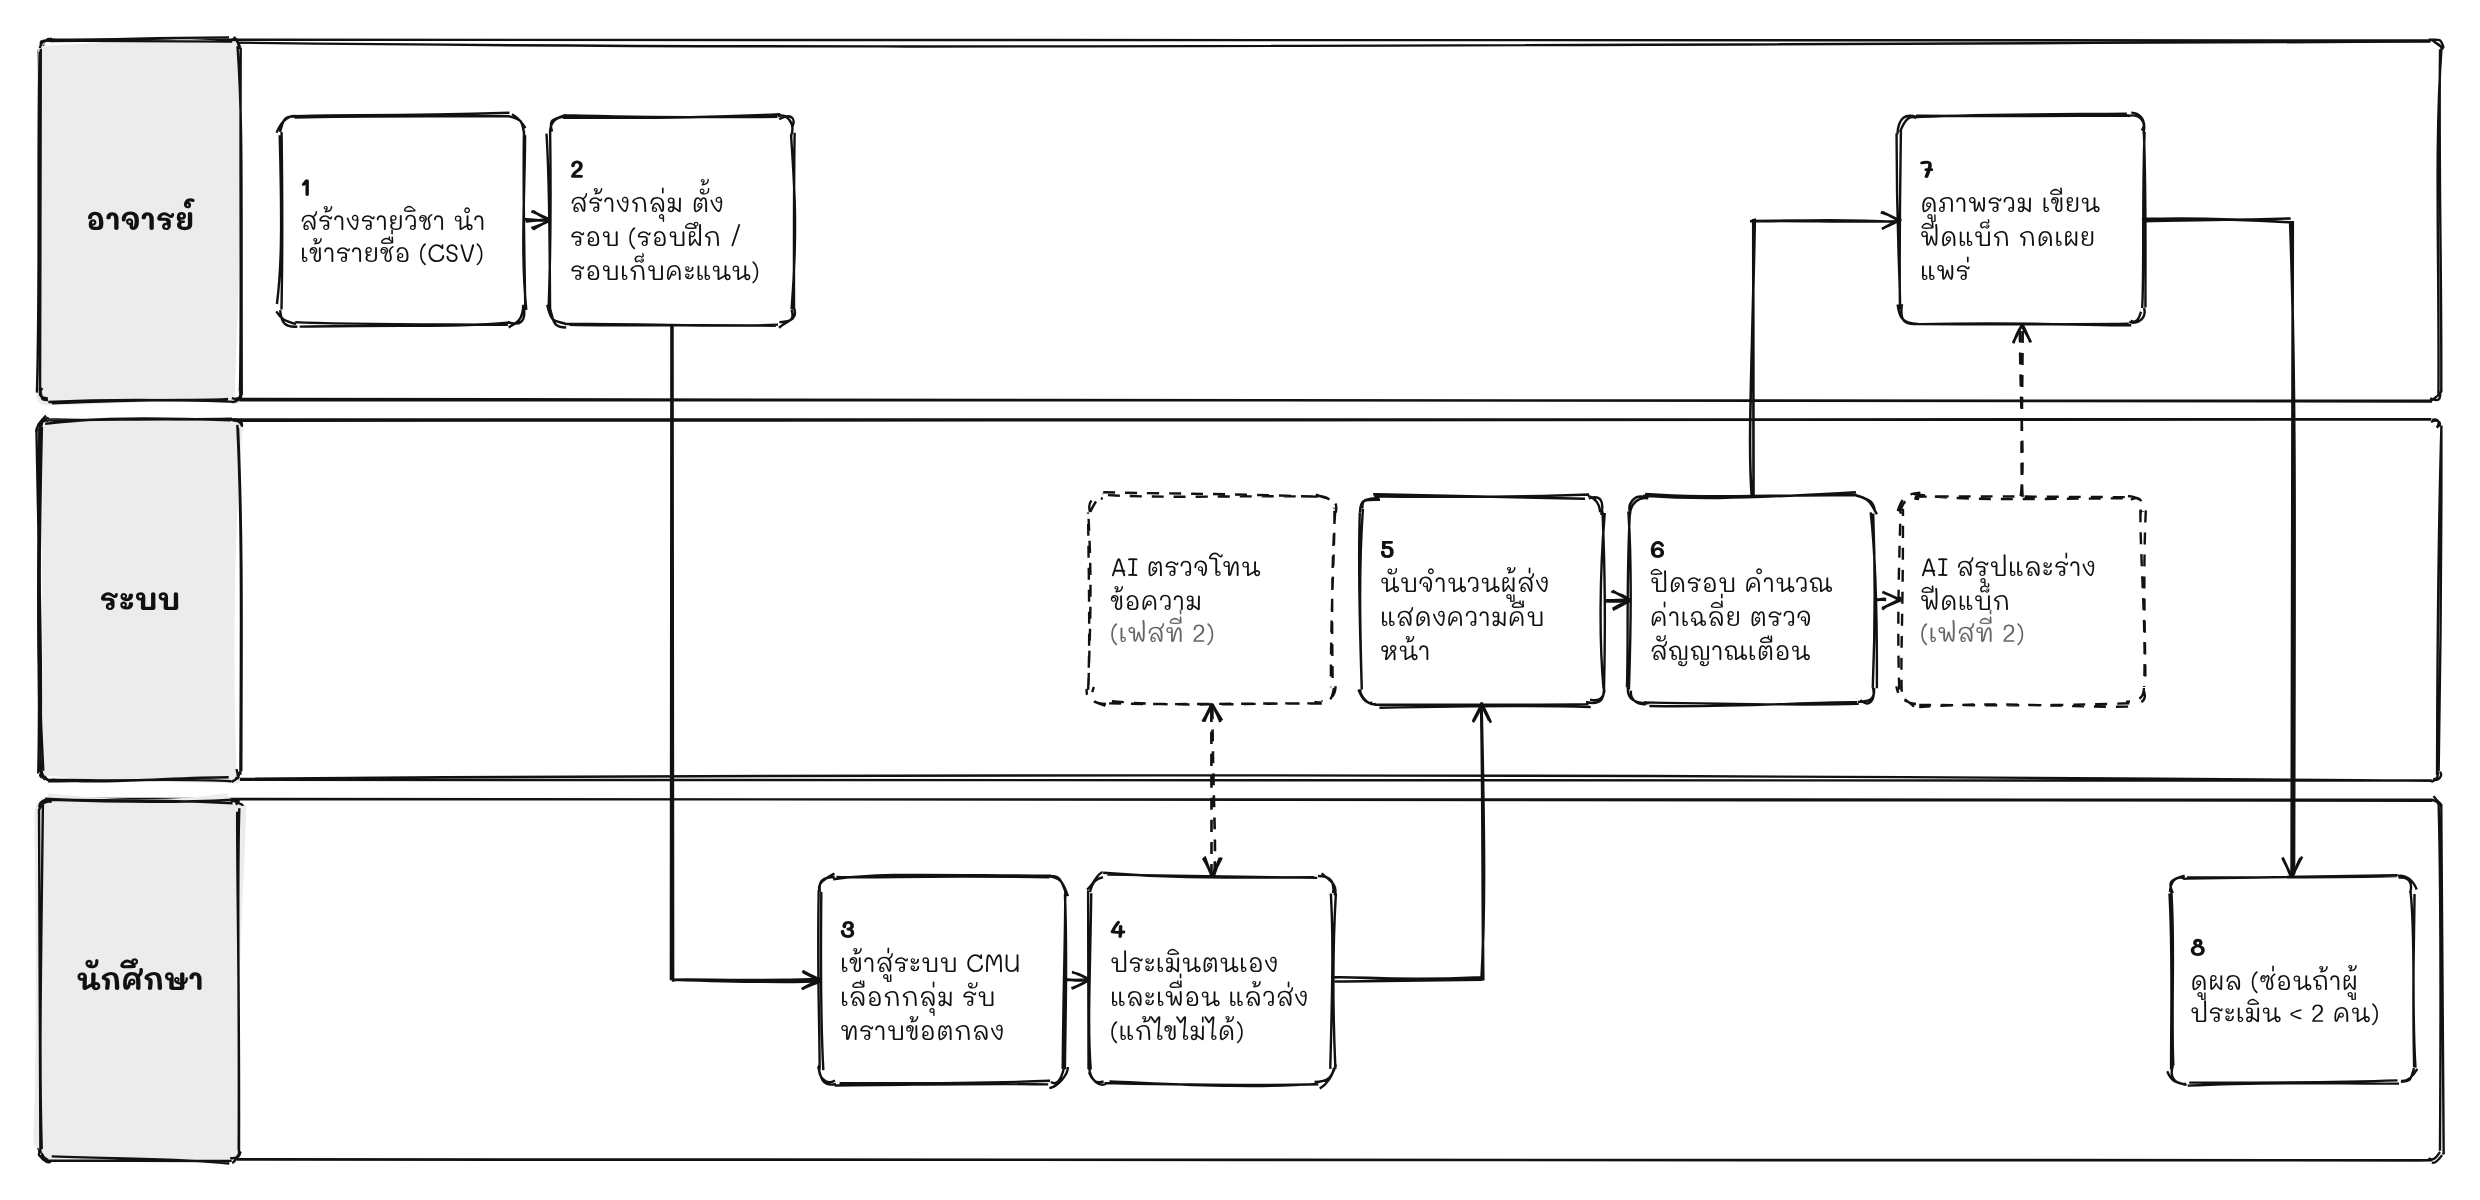
\includegraphics[width=\textwidth]{figures/ch3/fig3-1-swimlane.png}}{\fbox{\parbox{0.8\textwidth}{\centering\vspace{2cm}[วางไฟล์ figures/ch3/fig3-1-swimlane.png]\vspace{2cm}}}}
\caption{ขั้นตอนการทำงานของหนึ่งรอบประเมินแบบ swimlane}\label{fig:ch3-1}
\end{figure}

\subsection{การปกปิดตัวตนและสิทธิ์การมองเห็นข้อมูล}\label{sec:3.5.3}

ระบบไม่เปิดเผยตัวตนของผู้ประเมินต่อเพื่อน เพื่อให้นักศึกษากล้าให้ข้อเสนอแนะอย่างจริงใจ และให้นักศึกษาเห็นเฉพาะข้อมูลของตนเอง เพื่อลดการเปรียบเทียบและแข่งขันกันระหว่างเพื่อน สิทธิ์การมองเห็นข้อมูลแสดงในตารางที่~\ref{tab:ch3-8}

\begin{xltabular}{\textwidth}{|P{0.2\textwidth}|Y|P{0.12\textwidth}|Y|}
\caption{สิทธิ์การมองเห็นข้อมูลของผู้ใช้แต่ละบทบาท}\label{tab:ch3-8}\\
\hline \textbf{ข้อมูล} & \textbf{นักศึกษาเจ้าของข้อมูล} & \textbf{นักศึกษาคนอื่น} & \textbf{อาจารย์} \\ \hline
\endfirsthead
\multicolumn{4}{r}{\small (ต่อ)}\\ \hline \textbf{ข้อมูล} & \textbf{นักศึกษาเจ้าของข้อมูล} & \textbf{นักศึกษาคนอื่น} & \textbf{อาจารย์} \\ \hline
\endhead
คะแนนเฉลี่ยรายด้านที่เพื่อนประเมิน & เห็น เมื่อมีผู้ประเมินอย่างน้อย 2 คนและอาจารย์เผยแพร่แล้ว & ไม่เห็น & เห็น \\ \hline
คะแนนรายคนและชื่อผู้ประเมิน & ไม่เห็น & ไม่เห็น & เห็น เพื่อใช้ติดตามและกลั่นกรอง \\ \hline
ความเห็นปลายเปิด & เห็นหลังอาจารย์เผยแพร่ ในรูปแบบที่อาจารย์เลือก & ไม่เห็น & เห็นทั้งหมด \\ \hline
คะแนนที่ประเมินตนเอง & เห็น & ไม่เห็น & เห็น \\ \hline
สัญญาณเตือนและสถานะการส่ง & ไม่เห็น & ไม่เห็น & เห็น \\ \hline
\end{xltabular}

เงื่อนไขผู้ประเมินขั้นต่ำ 2 คนป้องกันไม่ให้นักศึกษาเดาได้ว่าใครเป็นผู้ประเมินในกรณีที่กลุ่มมีสมาชิกน้อย การบังคับสิทธิ์ทั้งหมดทำที่ฝั่ง API ไม่ใช่เพียงการซ่อนบนหน้าจอ ข้อมูลที่ผู้ใช้ไม่มีสิทธิ์จึงไม่ถูกส่งออกจากเซิร์ฟเวอร์เลย

\subsection{สัญญาณเตือน การเผยแพร่ผล และการสื่อสาร}\label{sec:3.5.4}

ในระยะที่ 1 ระบบสร้างสัญญาณเตือนจากรูปแบบคะแนนตามเงื่อนไขที่กำหนดไว้ (rule-based) เช่น คะแนนเฉลี่ยที่เพื่อนให้ต่ำในด้านใดด้านหนึ่ง คะแนนที่ประเมินตนเองต่างจากที่เพื่อนประเมินมาก หรือยังไม่ส่งแบบประเมิน เพื่อชี้ให้อาจารย์รู้ว่าควรดูแลทีมใดก่อน ฐานข้อมูลเก็บแหล่งที่มาของสัญญาณไว้ด้วย จึงรองรับสัญญาณจากปัญญาประดิษฐ์ (AI) ในระยะที่ 2 ได้โดยไม่ต้องเปลี่ยนโครงสร้าง

ผลการประเมินจะไม่ถึงนักศึกษาโดยอัตโนมัติ อาจารย์เป็นผู้ตรวจทานและกดเผยแพร่ทุกครั้ง โดยเลือกได้ว่าจะแสดงความเห็นของเพื่อนตามจริง หรือแสดงเป็นข้อสรุปที่อาจารย์เขียน การสื่อสารเป็นแบบทางเดียว นักศึกษาตอบกลับความเห็นของเพื่อนในระบบไม่ได้ เพราะการโต้ตอบอาจทำให้สืบทราบตัวตนผู้ประเมินได้ หากนักศึกษามีข้อสงสัยให้สื่อสารผ่านอาจารย์ นอกจากนี้ระบบออกแบบให้ใช้ร่วมกับกิจกรรมในชั้นเรียน เช่น อาจารย์อาจจัดเวลาประมาณ 1 ชั่วโมงให้นักศึกษาพูดคุยเรื่องข้อเสนอแนะกันแบบพบหน้า เพื่อไม่ให้การให้ข้อเสนอแนะผ่านระบบออนไลน์เพียงอย่างเดียวดูห่างเหิน

\section{การออกแบบส่วน AI (ระยะที่ 2)}\label{sec:3.6}

\subsection{ที่มาของการใช้ปัญญาประดิษฐ์}\label{sec:3.6.1}

การเรียนรู้ในปัจจุบันต้องปรับตัวกับการที่ทั้งผู้เรียนและผู้สอนใช้เครื่องมือปัญญาประดิษฐ์ (AI) มากขึ้น ระบบจึงนำปัญญาประดิษฐ์ มาใช้เฉพาะงานที่ปัญญาประดิษฐ์ (AI) ทำได้ดีและลดภาระคนได้จริง คือการอ่านและสรุปข้อความจำนวนมาก และการช่วยเกลาภาษา โดยไม่ให้ปัญญาประดิษฐ์ (AI) ตัดสินใจแทนคน ส่วนปัญญาประดิษฐ์ (AI) จัดอยู่ในการพัฒนาระยะที่ 2 โดยระบบใช้โมเดลภาษา Qwen ผ่าน API และแบ่งเป็น 2 ส่วน ดังรูปที่~\ref{fig:ch3-2}

\begin{figure}[htbp]
\centering
\IfFileExists{figures/ch3/fig3-2-ai.png}{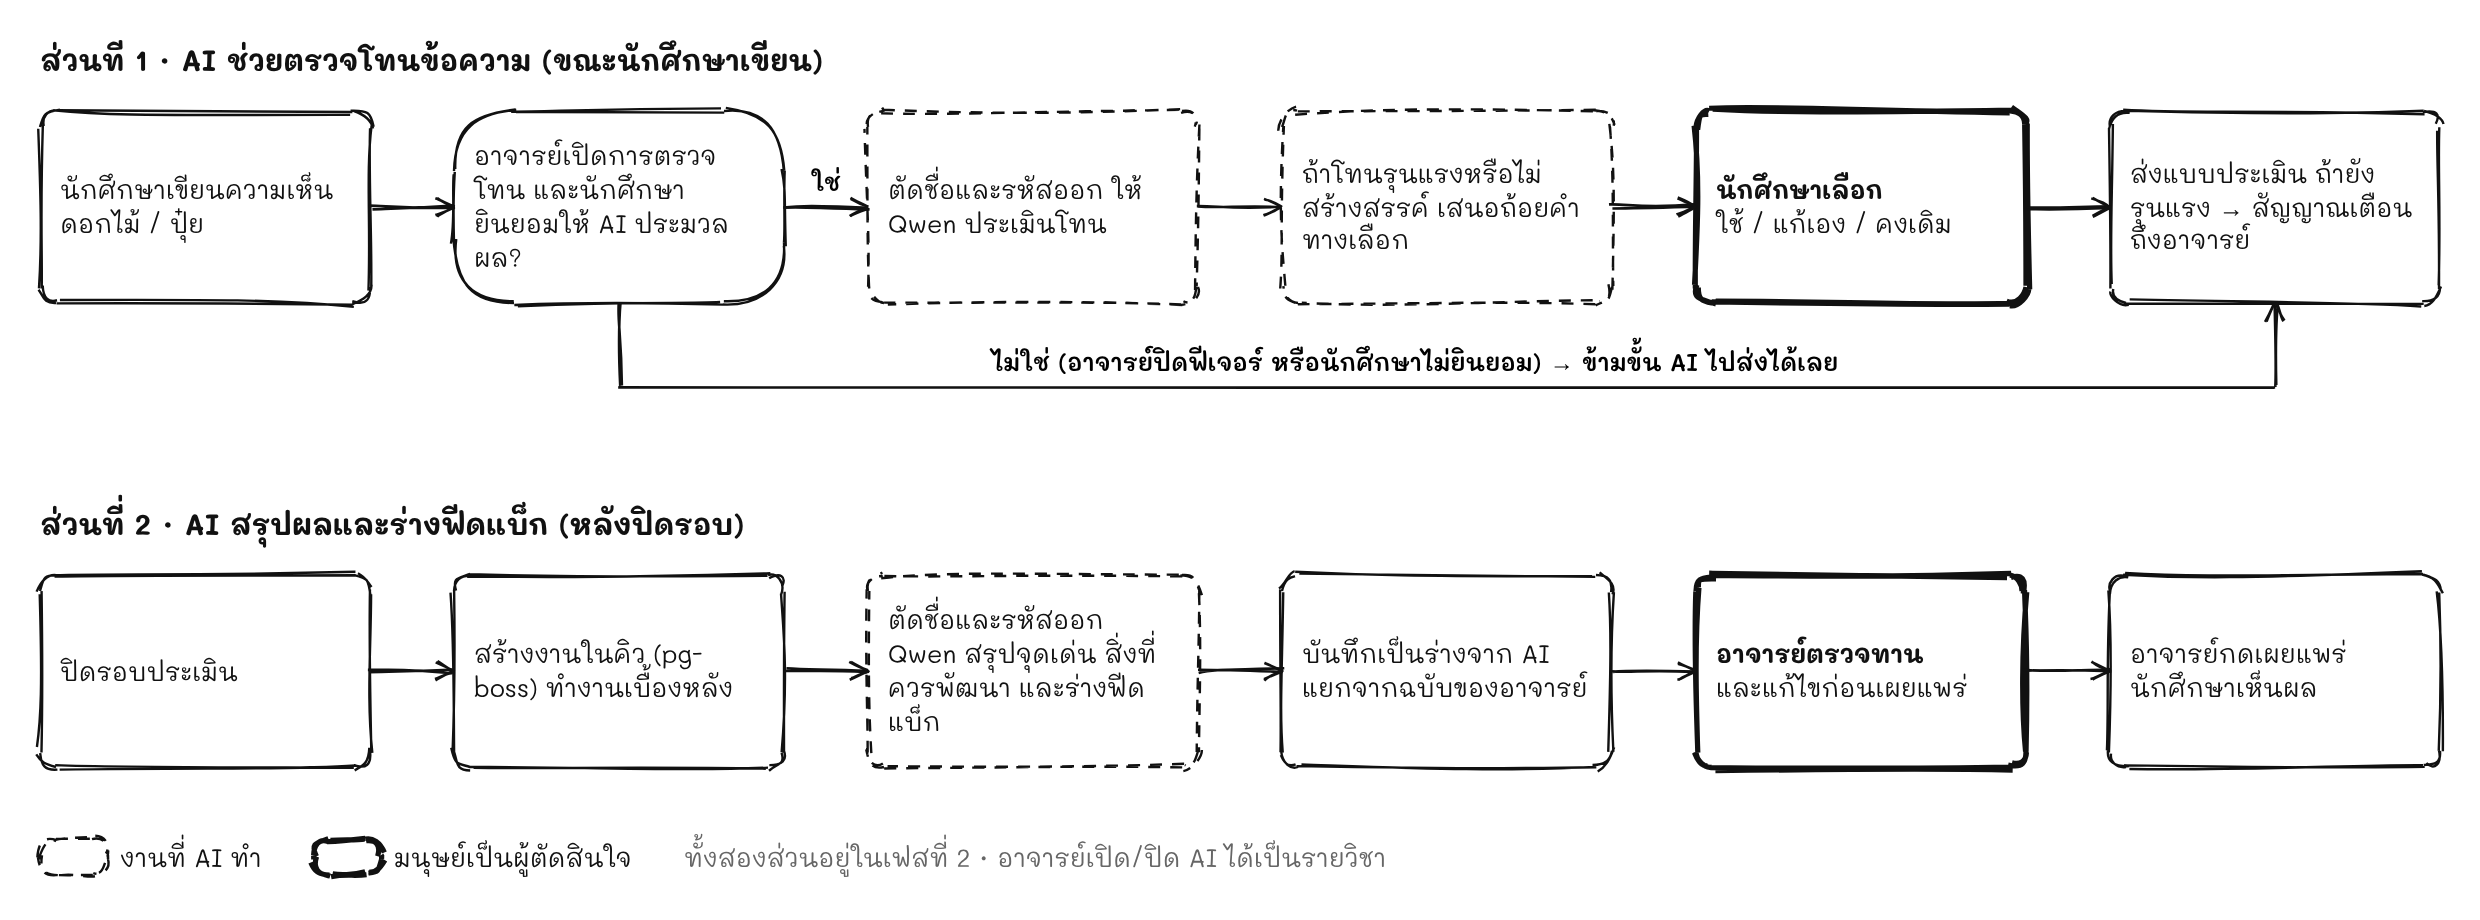
\includegraphics[width=\textwidth]{figures/ch3/fig3-2-ai.png}}{\fbox{\parbox{0.8\textwidth}{\centering\vspace{2cm}[วางไฟล์ figures/ch3/fig3-2-ai.png]\vspace{2cm}}}}
\caption{การทำงานของส่วน AI ทั้ง 2 ส่วน}\label{fig:ch3-2}
\end{figure}

\subsection{ปัญญาประดิษฐ์ช่วยตรวจโทนข้อความ}\label{sec:3.6.2}

อาจารย์เลือกเปิดหรือปิดฟีเจอร์นี้ได้เป็นรายวิชา เมื่อเปิดใช้งาน ขณะนักศึกษาเขียนความเห็นปลายเปิด ระบบส่งข้อความให้โมเดลประเมินโทน หากข้อความมีลักษณะรุนแรง ตำหนิตัวบุคคล หรือไม่สร้างสรรค์ ระบบจะแสดงคำเตือนพร้อมเสนอถ้อยคำทางเลือกที่สื่อประเด็นเดิมอย่างสร้างสรรค์ นักศึกษาเป็นผู้ตัดสินใจเองว่าจะใช้ถ้อยคำที่เสนอ แก้ไขเอง หรือคงข้อความเดิม ระบบไม่เปลี่ยนข้อความให้โดยอัตโนมัติ หากข้อความที่ส่งแล้วยังมีโทนรุนแรง ระบบจะบันทึกเป็นสัญญาณเตือนให้อาจารย์เห็น หากอาจารย์ปิดฟีเจอร์นี้ นักศึกษาจะเขียนและส่งความเห็นได้ตามปกติโดยไม่ผ่านการตรวจโทน

\subsection{ปัญญาประดิษฐ์สรุปผลและร่างข้อเสนอแนะ}\label{sec:3.6.3}

เมื่อปิดรอบประเมิน ระบบรวบรวมความเห็นที่นักศึกษาแต่ละคนได้รับ แล้วส่งให้โมเดลสรุปเป็นจุดเด่นและสิ่งที่ควรพัฒนา พร้อมร่างข้อเสนอแนะถึงนักศึกษาคนนั้น ร่างจากปัญญาประดิษฐ์ (AI) ถูกเก็บแยกจากฉบับที่อาจารย์แก้ไข และอาจารย์ต้องตรวจทานก่อนเผยแพร่ทุกครั้ง การประมวลผลทำผ่านคิวงานเบื้องหลัง ผู้ใช้จึงไม่ต้องรอระหว่างที่โมเดลทำงาน

\subsection{หลักการกำกับการใช้ปัญญาประดิษฐ์ (AI)}\label{sec:3.6.4}

\begin{itemize}
  \item มนุษย์ตัดสินใจขั้นสุดท้ายเสมอ (human-in-the-loop): AI ทำหน้าที่เสนอ ส่วนนักศึกษาและอาจารย์เป็นผู้เลือก
  \item เปิดหรือปิดได้: อาจารย์เปิดหรือปิดฟีเจอร์ปัญญาประดิษฐ์ (AI) ได้เป็นรายวิชา และข้อความของนักศึกษาจะถูกส่งให้ปัญญาประดิษฐ์ (AI) เฉพาะเมื่อนักศึกษายินยอมในส่วนทางเลือก (หัวข้อ~\ref{sec:3.9.2})
  \item ลดข้อมูลที่ส่งออก: ส่งเฉพาะข้อความที่ต้องประมวลผล โดยไม่ส่งชื่อหรือรหัสนักศึกษาไปยังผู้ให้บริการโมเดล
  \item ยอมรับข้อจำกัด: โมเดลอาจตีความภาษาไทยผิด โดยเฉพาะถ้อยคำประชดประชันซึ่งจัดเป็นงานในระยะที่ 3 นี่คือเหตุผลที่ระบบไม่ให้ปัญญาประดิษฐ์ (AI) ตัดสินใจเอง
\end{itemize}

\section{สถาปัตยกรรมระบบและฐานข้อมูล}\label{sec:3.7}

\subsection{ภาพรวมสถาปัตยกรรม}\label{sec:3.7.1}

ระบบเป็นเว็บแอปพลิเคชันที่แยกส่วนหน้า (frontend) และส่วนหลัง (backend) ออกจากกัน และสื่อสารกันผ่าน REST API ด้วยข้อมูลรูปแบบ JSON องค์ประกอบหลักแสดงในรูปที่~\ref{fig:ch3-3} ดังนี้

\begin{itemize}
  \item ส่วนหน้า: React 19, Vite และ TypeScript จัดหน้าตาด้วย Tailwind CSS จัดการข้อมูลจากเซิร์ฟเวอร์ด้วย TanStack Query และจัดการสถานะภายในหน้าเว็บด้วย Zustand
  \item เว็บเซิร์ฟเวอร์: nginx ให้บริการไฟล์ของส่วนหน้า ทำหน้าที่ reverse proxy ไปยัง API และจัดการ HTTPS
  \item ส่วนหลัง: Node.js และ Express 5 เข้าถึงฐานข้อมูลผ่าน Drizzle ORM และกำหนดสัญญาการเชื่อมต่อ API ด้วย OpenAPI
  \item ฐานข้อมูล: PostgreSQL เก็บข้อมูลของระบบ เซสชันผู้ใช้ และคิวงานเบื้องหลัง (pg-boss)
  \item Worker และบริการ AI (เฟสที่ 2): worker ดึงงานจากคิวไปเรียกโมเดล Qwen ผ่าน API แล้วบันทึกผลกลับลงฐานข้อมูล
\end{itemize}

คณะผู้จัดทำเลือกใช้ PostgreSQL เป็นทั้งที่เก็บเซสชันและคิวงาน แทนการเพิ่ม Redis และ BullMQ ซึ่งเป็นอีกทางเลือกหนึ่ง เพื่อลดจำนวนบริการที่ต้องดูแลและใช้ทรัพยากรน้อยลง ทางเลือกนี้เหมาะกับข้อจำกัดของเซิร์ฟเวอร์ขนาด 2 vCPU หน่วยความจำ 4 GB ตามงบประมาณของโครงงาน และปริมาณงานของระบบในระดับรายวิชาซึ่งไม่ได้ต้องการความเร็วที่สูงมาก

\begin{figure}[htbp]
\centering
\IfFileExists{figures/ch3/fig3-3-architecture.png}{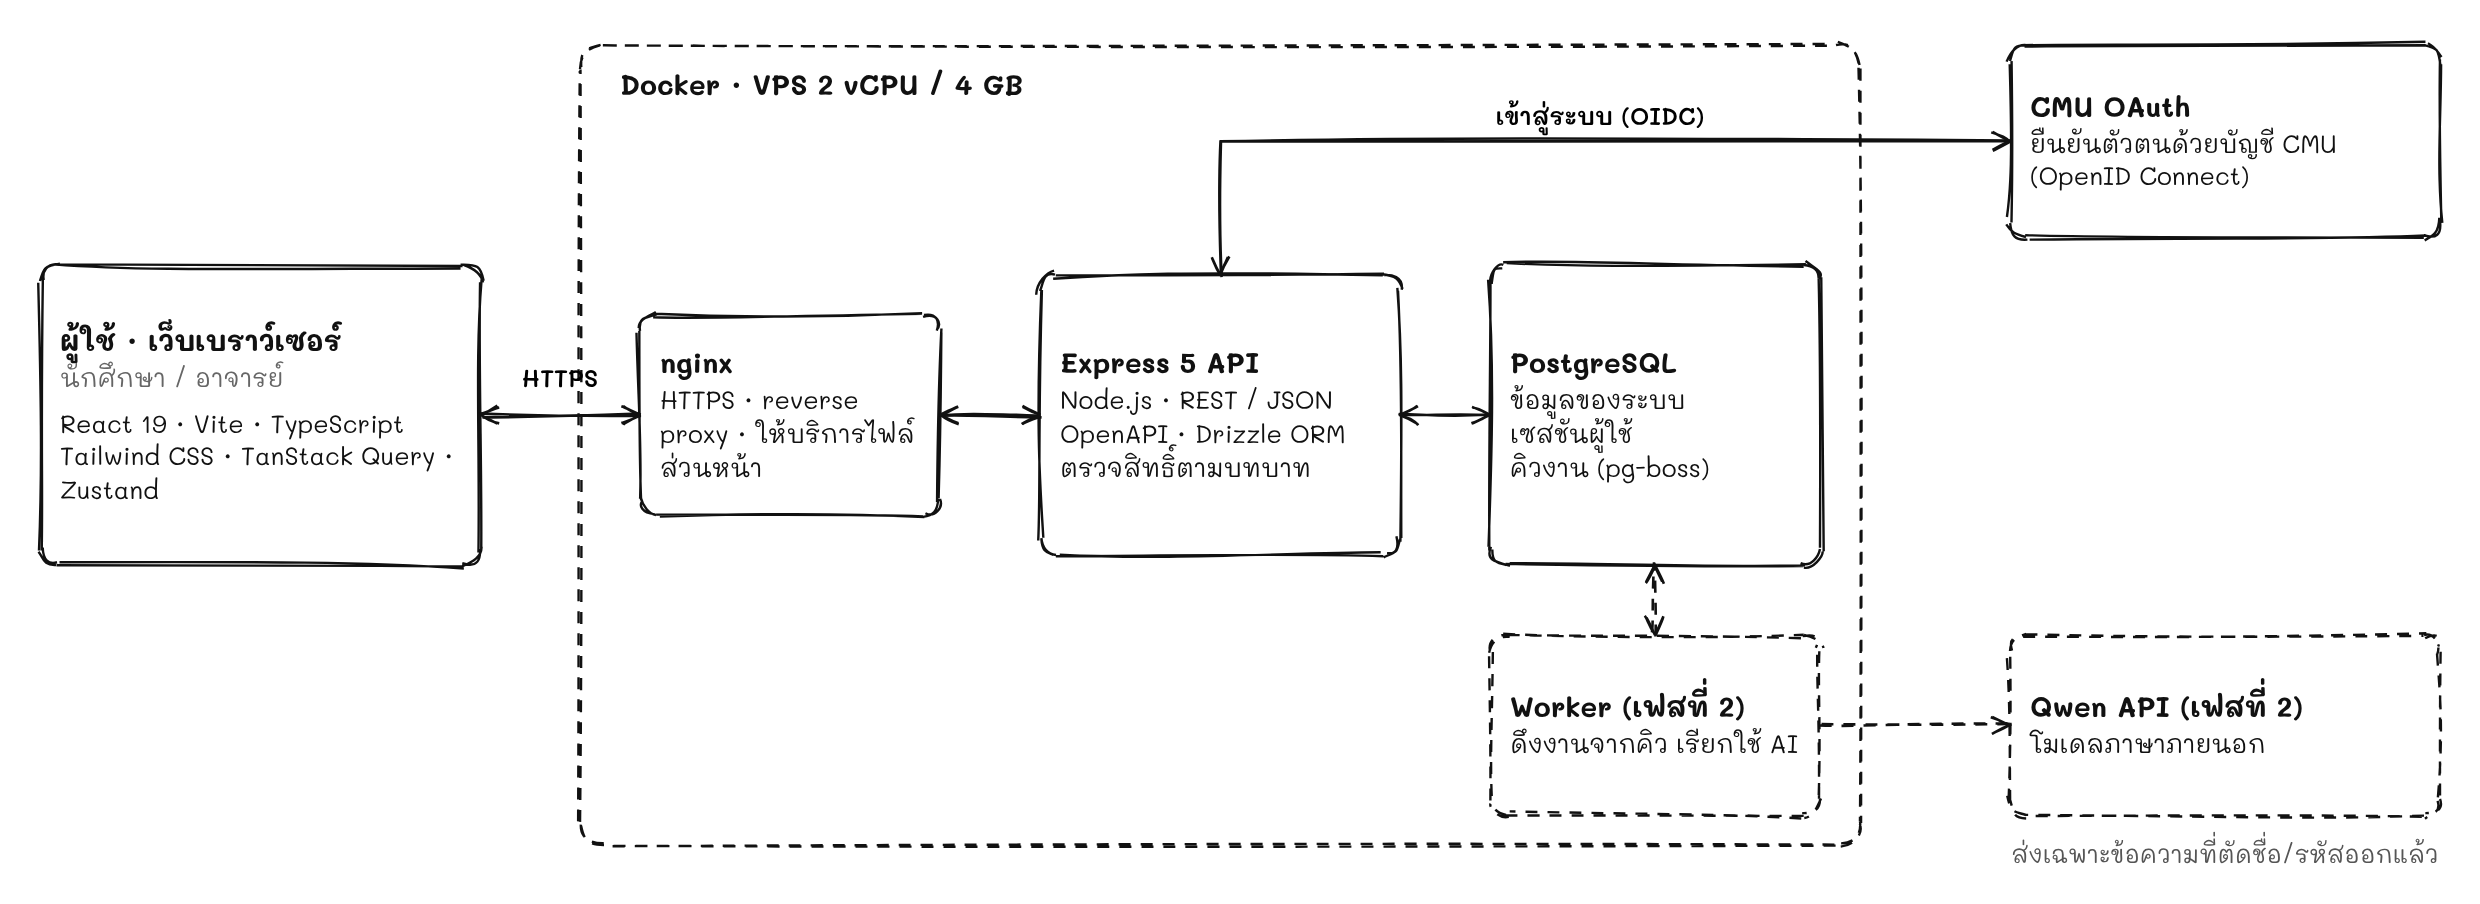
\includegraphics[width=\textwidth]{figures/ch3/fig3-3-architecture.png}}{\fbox{\parbox{0.8\textwidth}{\centering\vspace{2cm}[วางไฟล์ figures/ch3/fig3-3-architecture.png]\vspace{2cm}}}}
\caption{สถาปัตยกรรมของระบบ}\label{fig:ch3-3}
\end{figure}

\subsection{การยืนยันตัวตน}\label{sec:3.7.2}

ผู้ใช้เข้าสู่ระบบด้วยบัญชี CMU ผ่าน CMU OAuth ตามมาตรฐาน OpenID Connect~\cite{sakimura2014oidc} ระบบจึงไม่ต้องเก็บรหัสผ่านของผู้ใช้เอง หลังยืนยันตัวตน เซิร์ฟเวอร์สร้างเซสชันที่เก็บในฐานข้อมูล และส่งคุกกี้เซสชันแบบ HttpOnly และ Secure ให้เบราว์เซอร์ บทบาทของผู้ใช้ในแต่ละรายวิชา (นักศึกษาหรืออาจารย์) ถูกตรวจสอบทุกครั้งที่เรียก API

\subsection{การออกแบบฐานข้อมูล}\label{sec:3.7.3}

ฐานข้อมูลเป็นแบบเชิงสัมพันธ์ ประกอบด้วยตารางที่ระยะที่ 1 ใช้ และตารางที่เตรียมไว้สำหรับระยะถัดไป ได้แก่ ตารางสัญญาณเตือน (flags) และตารางสรุปผล (ai\_feedback\_summaries) สำหรับปัญญาประดิษฐ์ (AI) และตารางบันทึกการซิงก์ข้อมูล (external\_sync\_logs) สำหรับการเชื่อมต่อระบบภายนอก ความสัมพันธ์ของข้อมูลแสดงในรูปที่~\ref{fig:ch3-4} โดยมีการตัดสินใจออกแบบที่สำคัญดังนี้

\begin{itemize}
  \item ตารางคะแนน (ratings) ให้ช่องผู้ถูกประเมินเป็นค่าว่างได้ เพื่อรองรับคำถามระดับทีมที่ไม่ได้ประเมินบุคคลใดบุคคลหนึ่ง
  \item ตารางสรุปผล (ai\_feedback\_summaries) เก็บทั้งร่างจากปัญญาประดิษฐ์ (AI) และฉบับสุดท้ายที่อาจารย์แก้ไข เพื่อแยกให้เห็นว่าส่วนใดมาจากปัญญาประดิษฐ์ (AI) และส่วนใดผ่านการตรวจทานแล้ว
  \item ตารางความยินยอม (consents) เก็บเวอร์ชันของนโยบายที่ผู้ใช้ยินยอม เพื่อขอความยินยอมใหม่ได้เมื่อนโยบายเปลี่ยน
  \item ตารางสัญญาณเตือน (flags) มีช่องระบุแหล่งที่มาของสัญญาณ เพื่อรองรับทั้งสัญญาณจากเงื่อนไขคะแนนและจากปัญญาประดิษฐ์ (AI)
  \item ตารางรายวิชาและผู้ใช้มีช่องเก็บรหัสอ้างอิงจากระบบภายนอก เพื่อเตรียมเชื่อมต่อ Mango Canvas ในระยะที่ 3 โดยมีตารางบันทึกการซิงก์ข้อมูล (external\_sync\_logs) เก็บผลการนำเข้ารายชื่อและส่งออกคะแนนของแต่ละรายวิชา
  \item ตารางระดับเกณฑ์การให้คะแนน (rubric\_levels) เก็บคำอธิบายพฤติกรรมของแต่ละคะแนนในคำถามแบบให้คะแนน เพื่อให้ผู้ประเมินใช้เกณฑ์เดียวกัน
\end{itemize}

\begin{sidewaysfigure}
\centering
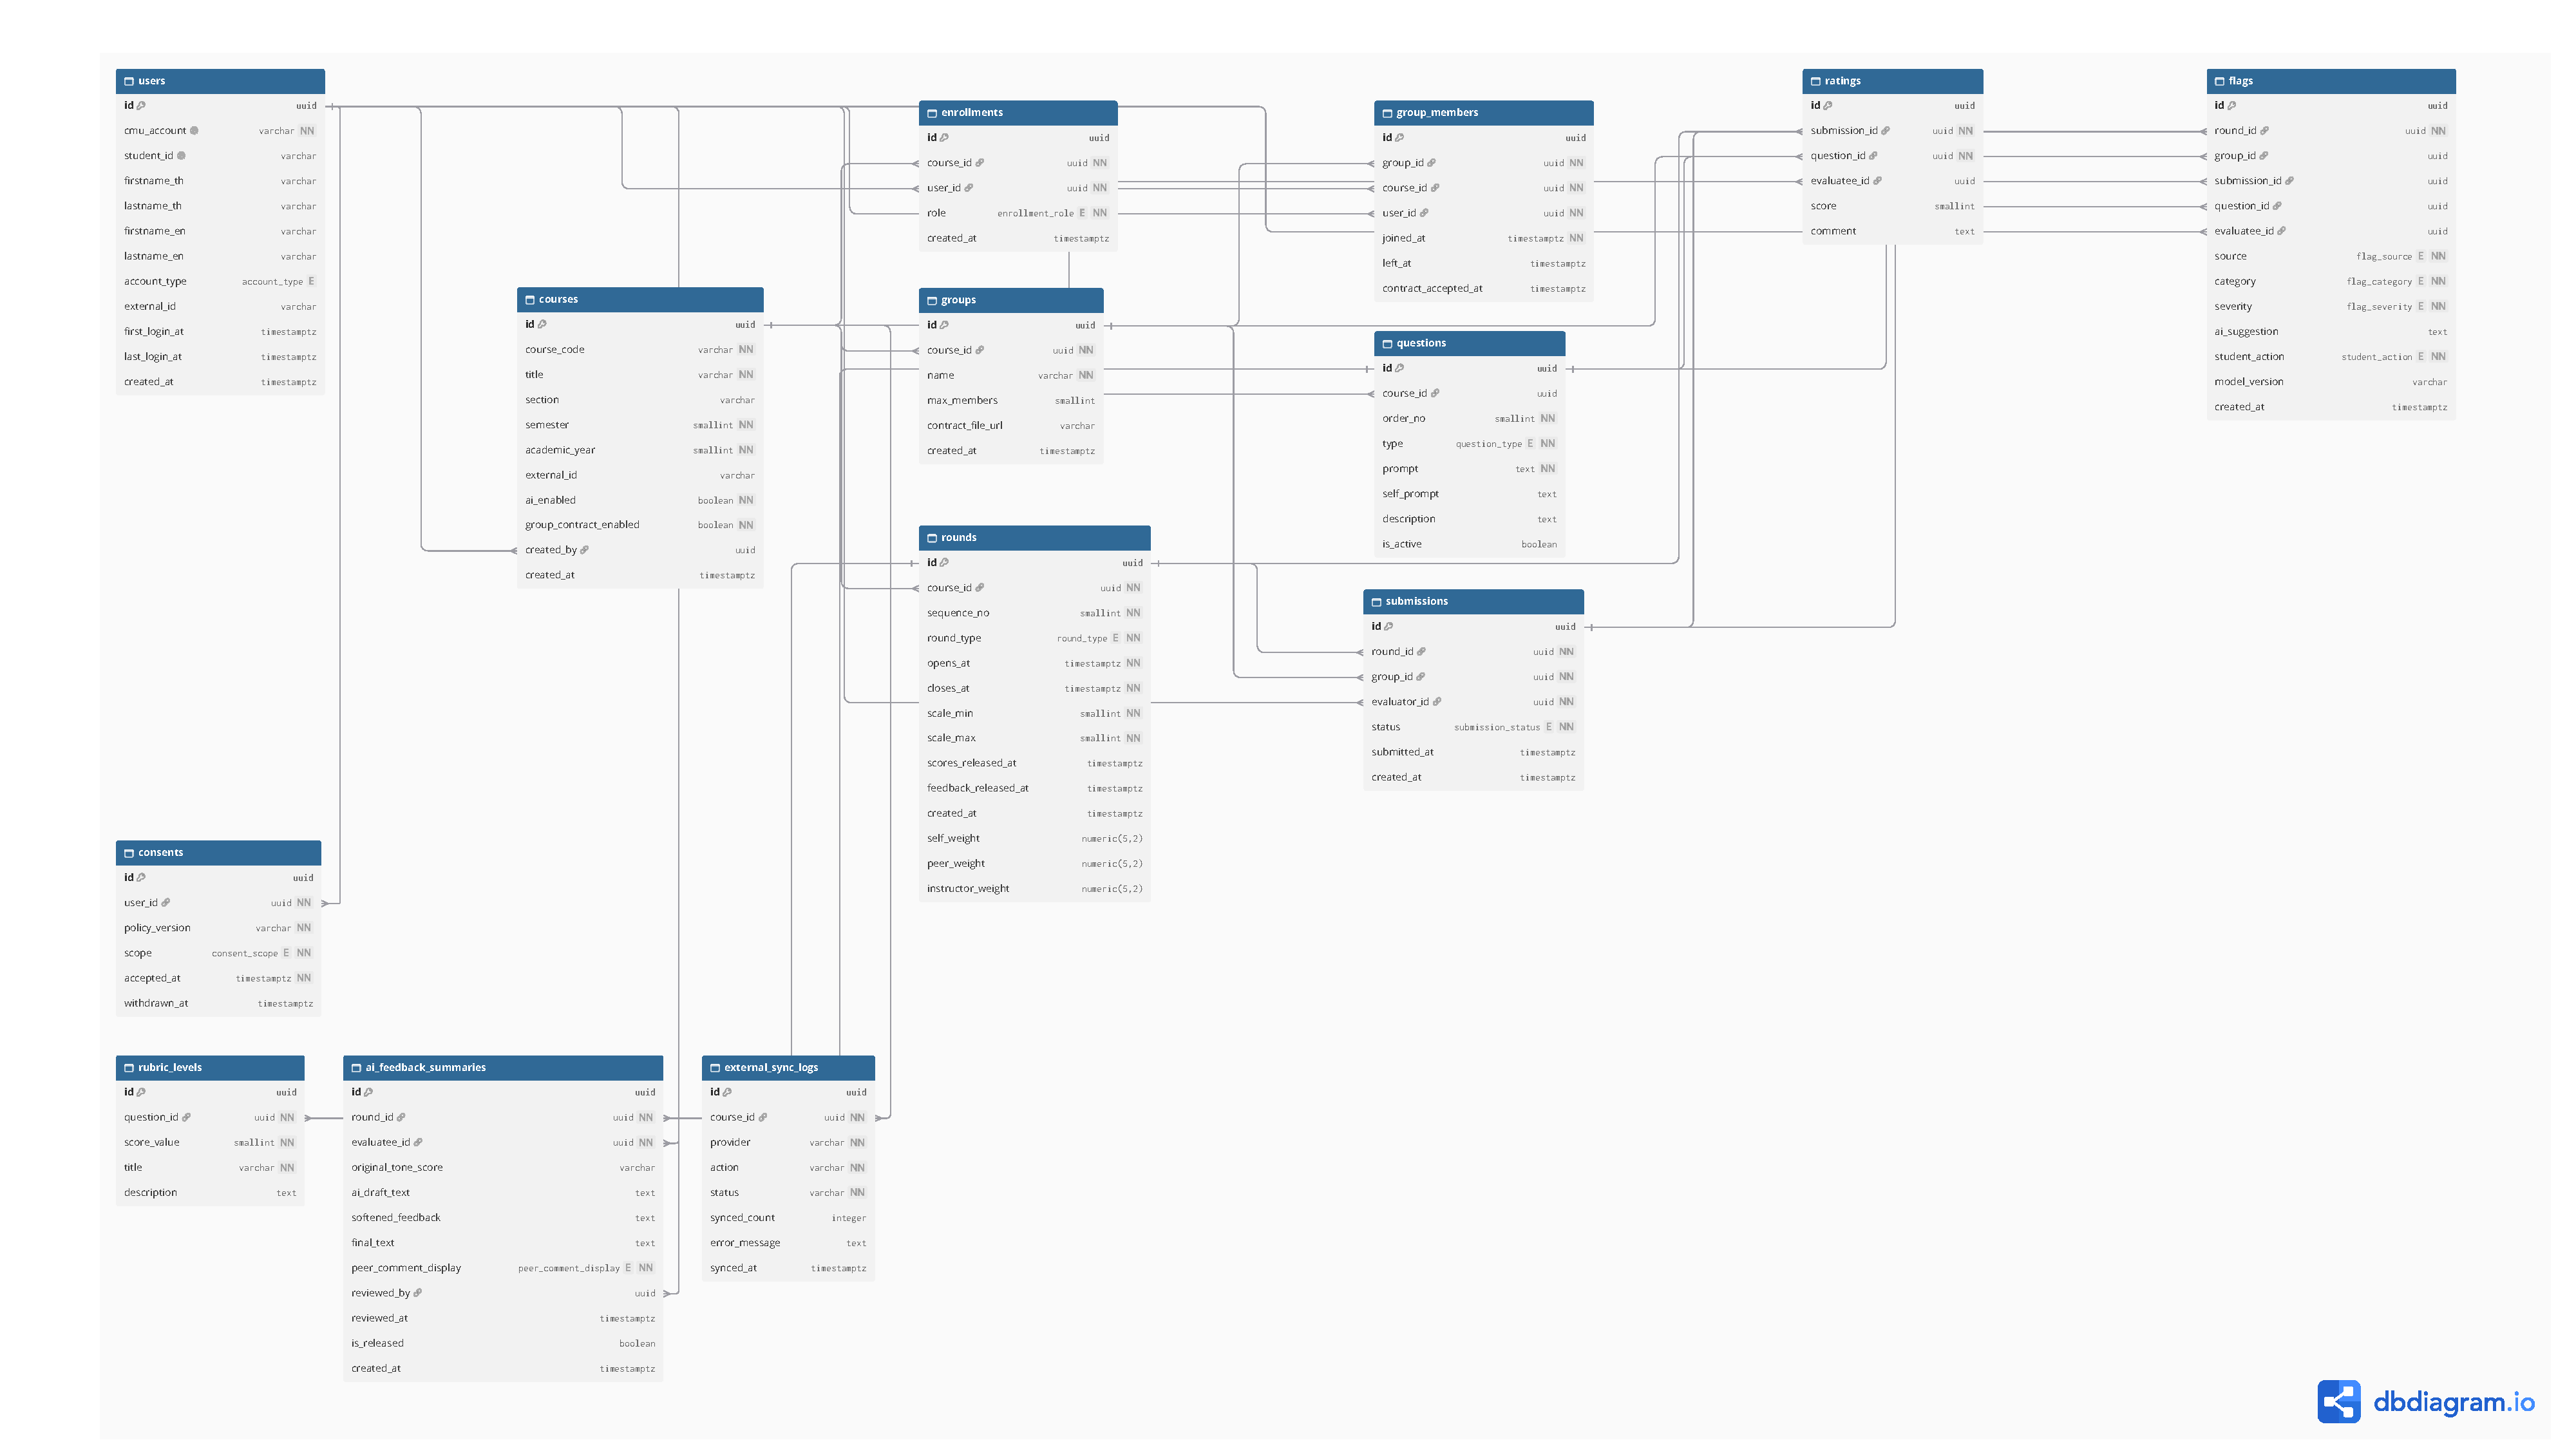
\includegraphics[width=\linewidth]{figures/ch3/fig3-4-er.pdf}
\caption{แผนภาพความสัมพันธ์ของข้อมูล (ER diagram)}\label{fig:ch3-4}
\end{sidewaysfigure}

\subsection{การติดตั้งและการทดสอบ}\label{sec:3.7.4}

ทุกบริการถูกบรรจุเป็น Docker container และติดตั้งบนเซิร์ฟเวอร์เสมือน (VPS) ขนาด 2 vCPU หน่วยความจำ 4 GB การทดสอบใช้ Vitest สำหรับ unit test และ integration test และใช้ Cypress สำหรับ end-to-end test ส่วนการสำรองข้อมูล การตรวจสอบสถานะระบบ และการส่งอีเมล ใช้บริการแบบไม่มีค่าใช้จ่าย

\section{การออกแบบส่วนต่อประสานผู้ใช้}\label{sec:3.8}

\subsection{หลักการออกแบบ}\label{sec:3.8.1}

\begin{itemize}
  \item นำทางตามงาน: แถบเมนูด้านข้างจัดตามงานที่ผู้ใช้ต้องทำ พร้อมตัวเลขแจ้งจำนวนงานค้าง
  \item แสดงสถานะด้วยป้ายสถานะ (status pill) เช่น เปิดรับ ปิดแล้ว และรอเผยแพร่
  \item แบบประเมินแสดงทีละคำถามต่อหน้าจอ เพื่อลดภาระการอ่านและใช้งานบนมือถือได้สะดวก
  \item ออกแบบตามแนวทาง WCAG 2.2~\cite{w3c2023wcag} เช่น ความต่างของสีตัวอักษรกับพื้นหลังที่เพียงพอ การใช้งานด้วยแป้นพิมพ์ และการติดป้ายกำกับช่องกรอกทุกช่อง
\end{itemize}

หน้าจอทั้งหมดออกแบบเป็นต้นแบบความละเอียดต่ำ (low-fidelity wireframe) แบบขาวดำก่อนพัฒนาจริง และใช้ต้นแบบนี้สื่อสารทั้งภายในทีมและกับอาจารย์ผู้ใช้ เพื่อรับความคิดเห็นก่อนลงมือพัฒนา

\subsection{หน้าจอฝั่งนักศึกษา}\label{sec:3.8.2}

ผู้ใช้เข้าสู่ระบบด้วยบัญชี CMU ผ่าน CMU OAuth โดยไม่ต้องสร้างรหัสผ่านใหม่ ดังรูปที่~\ref{fig:ch3-5}

\begin{figure}[htbp]
\centering
\IfFileExists{figures/ch3/fig3-5-login.png}{
\includegraphics[width=\textwidth]{figures/ch3/fig3-5-login.png}}{\fbox{\parbox{0.8\textwidth}{\centering\vspace{2cm}[วางไฟล์ figures/ch3/fig3-5-login.png]\vspace{2cm}}}}
\caption{หน้าเข้าสู่ระบบ}\label{fig:ch3-5}
\end{figure}

ครั้งแรกที่เข้าใช้งาน นักศึกษาต้องอ่านข้อตกลงการใช้ข้อมูลส่วนบุคคล ซึ่งแบ่งจอเป็น 2 ส่วน ด้านซ้ายย้ำว่าความเห็นถึงเพื่อนจะไม่ระบุชื่อ ด้านขวาแสดงว่าเก็บข้อมูลอะไร ใครเห็น เก็บนานเท่าใด และสิทธิ์ของเจ้าของข้อมูล พร้อมตัวเลือกส่วนจำเป็นและส่วนทางเลือก ดังรูปที่~\ref{fig:ch3-6}

\begin{figure}[htbp]
\centering
\IfFileExists{figures/ch3/fig3-6-consent.png}{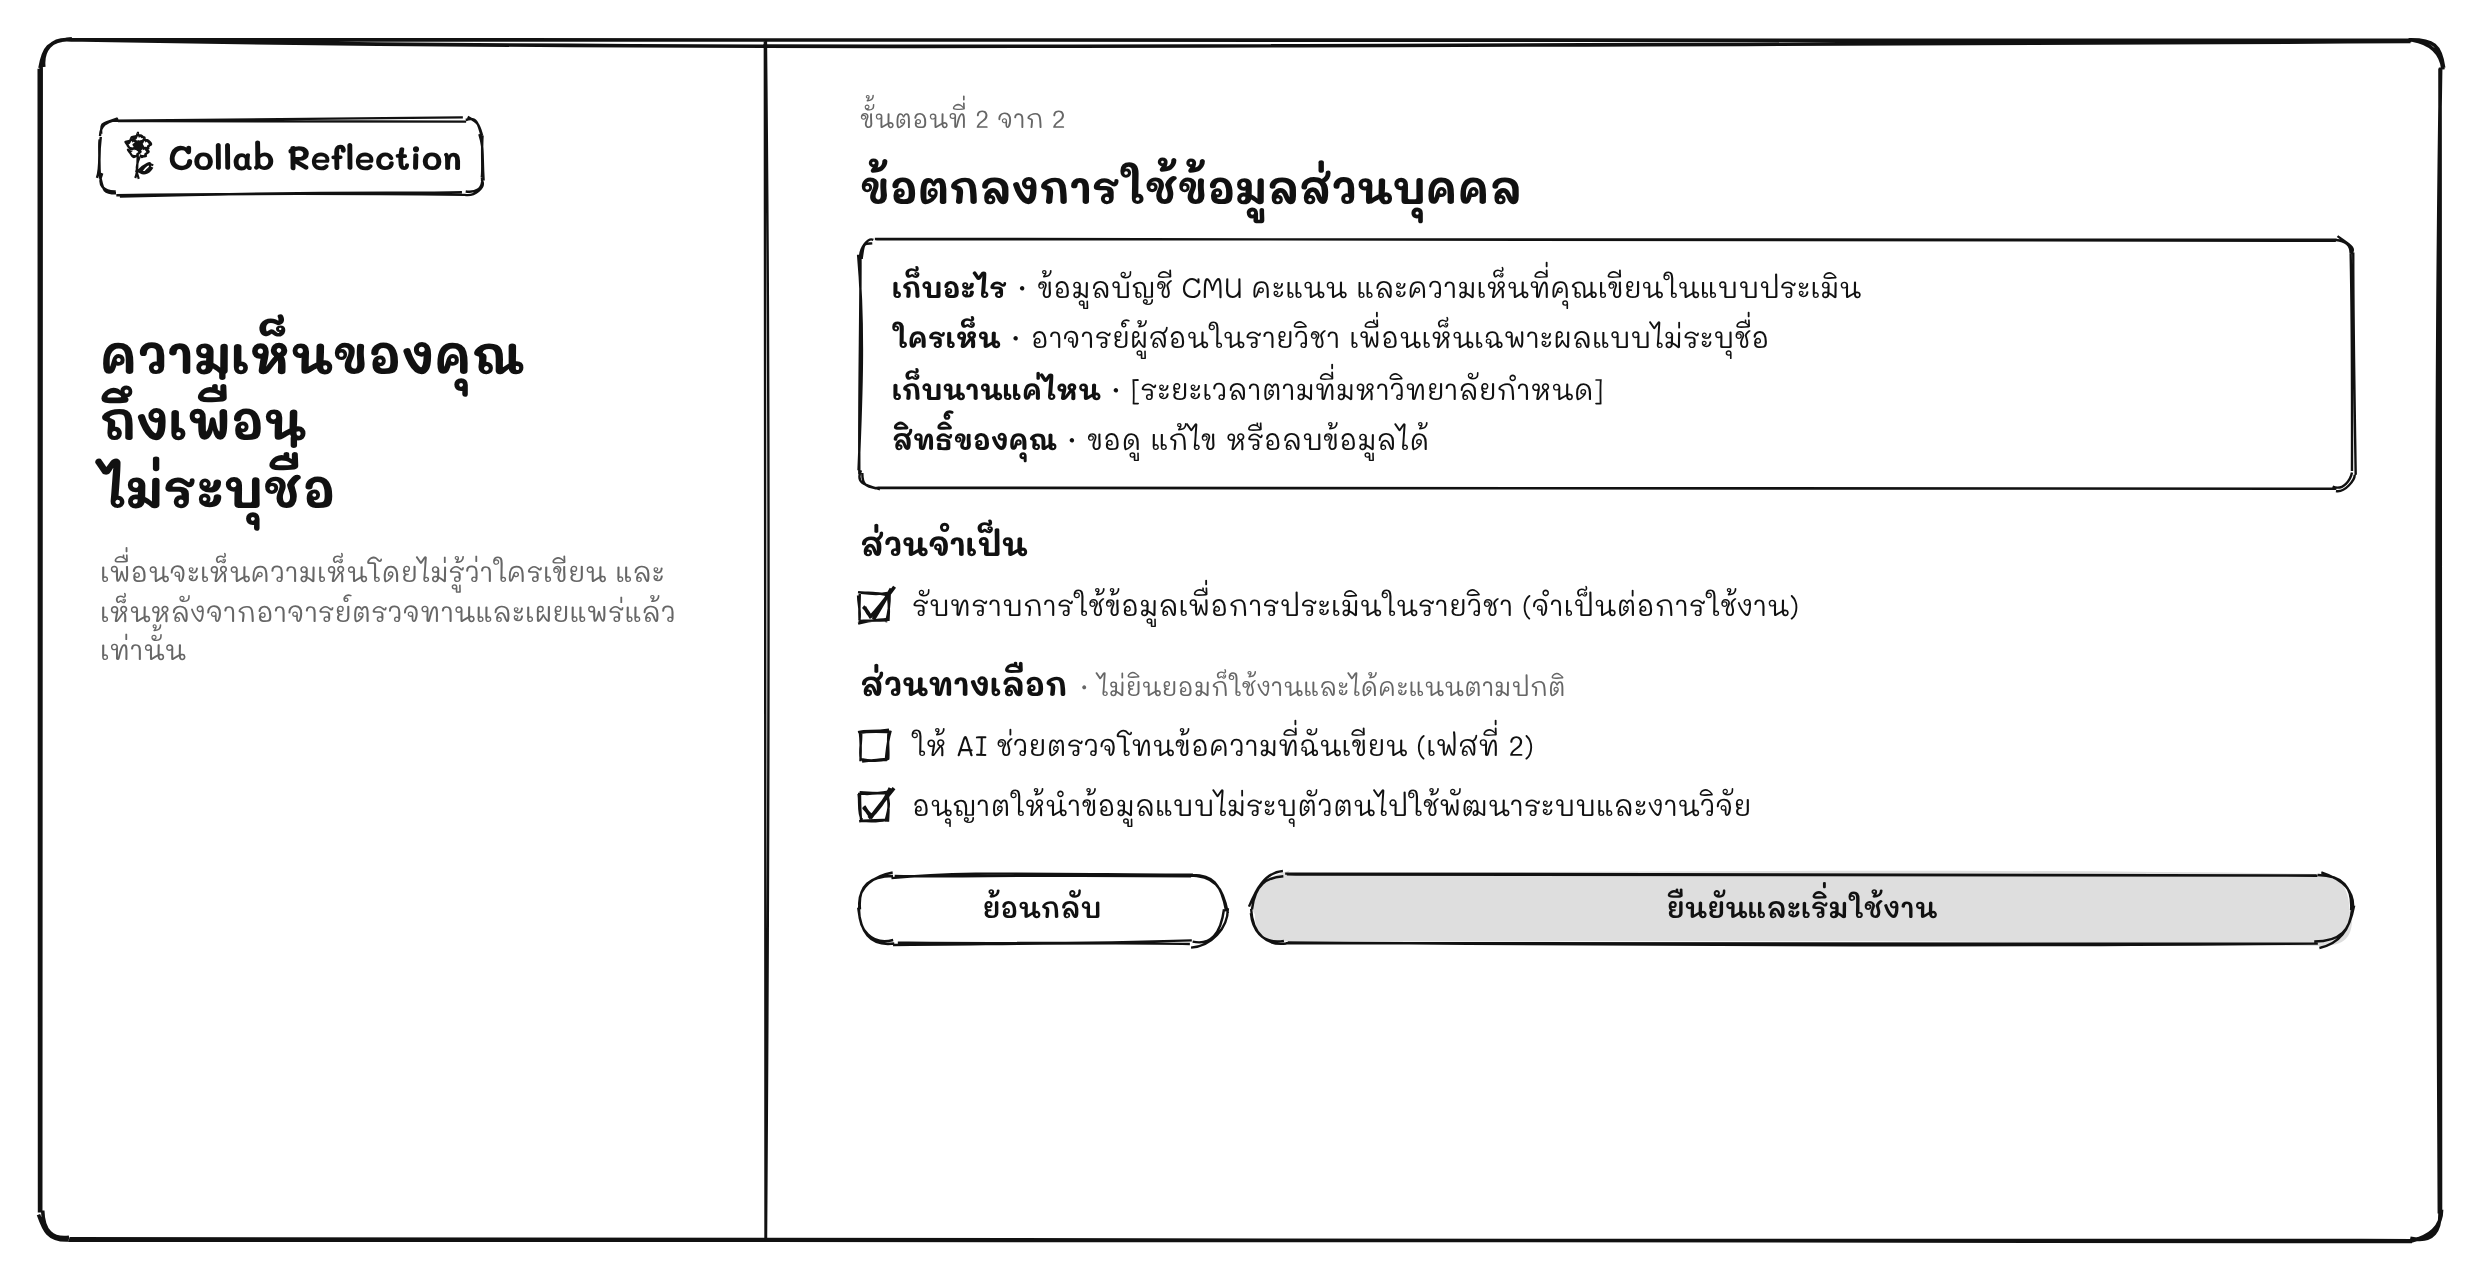
\includegraphics[width=\textwidth]{figures/ch3/fig3-6-consent.png}}{\fbox{\parbox{0.8\textwidth}{\centering\vspace{2cm}[วางไฟล์ figures/ch3/fig3-6-consent.png]\vspace{2cm}}}}
\caption{หน้าข้อตกลงการใช้ข้อมูลส่วนบุคคล}\label{fig:ch3-6}
\end{figure}

หน้ารายวิชาแสดงกลุ่มของนักศึกษา ข้อตกลงกลุ่ม และรายการรอบประเมิน โดยทุกรอบมีป้ายบอกว่าเป็นรอบฝึกหรือรอบเก็บคะแนน พร้อมสถานะของรอบ ดังรูปที่~\ref{fig:ch3-7}

\begin{figure}[htbp]
\centering
\IfFileExists{figures/ch3/fig3-7-student-course.png}{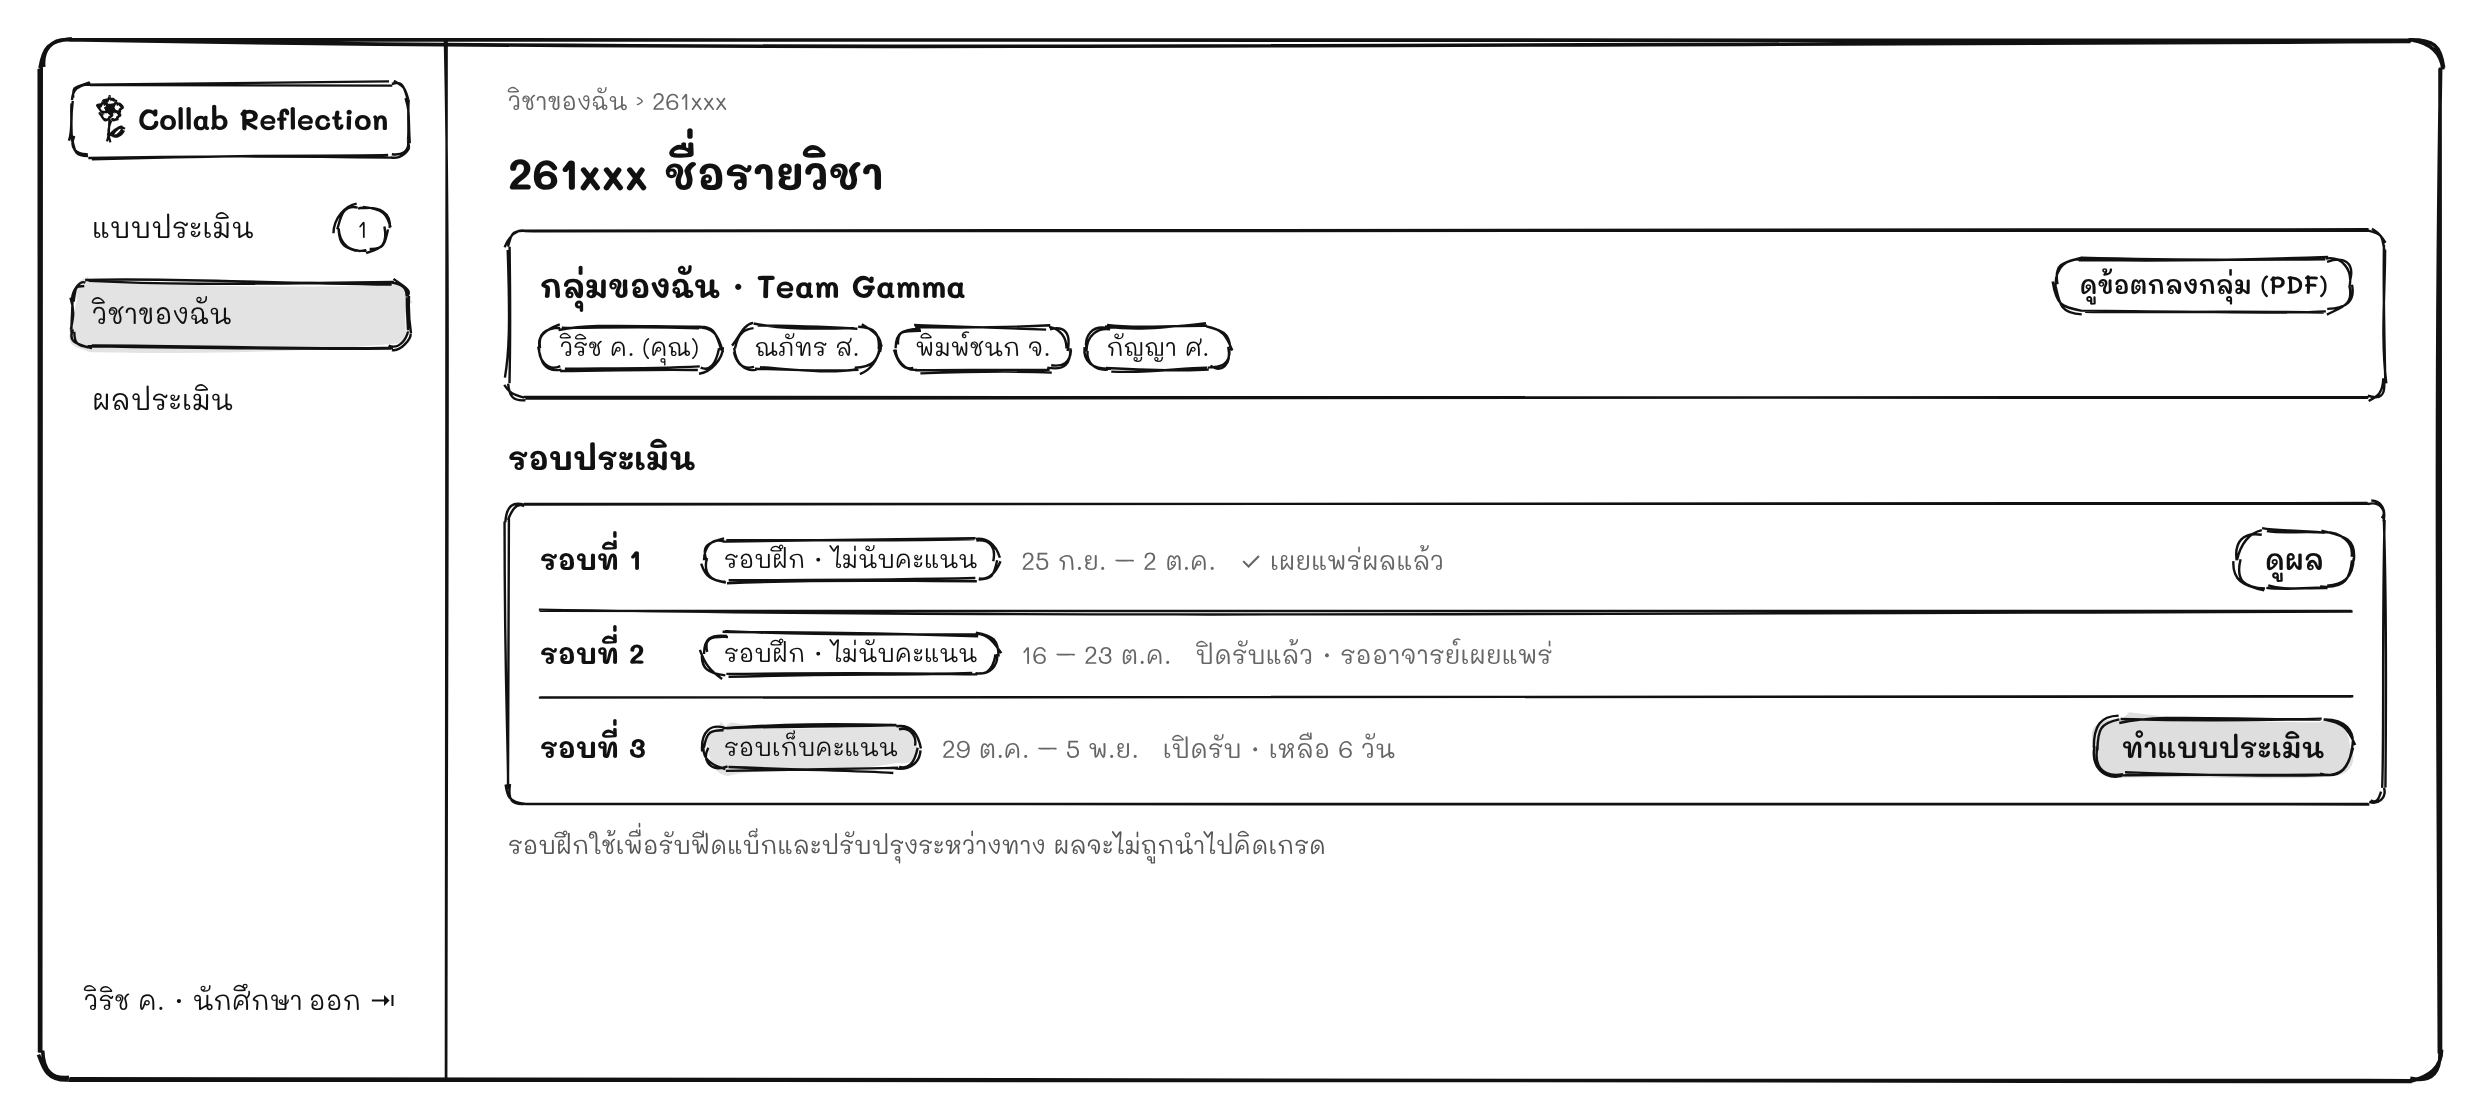
\includegraphics[width=\textwidth]{figures/ch3/fig3-7-student-course.png}}{\fbox{\parbox{0.8\textwidth}{\centering\vspace{2cm}[วางไฟล์ figures/ch3/fig3-7-student-course.png]\vspace{2cm}}}}
\caption{หน้ารายวิชาและรอบประเมินของนักศึกษา}\label{fig:ch3-7}
\end{figure}

แบบประเมินแสดงทีละด้านต่อหน้าจอ ด้านบนมีคำอธิบายพฤติกรรมของระดับ 1, 3 และ 5 ให้นักศึกษาให้คะแนนสมาชิกทุกคนรวมถึงตนเอง และด้านขวามีแถบแสดงขั้นตอนทั้ง 7 ขั้น ดังรูปที่~\ref{fig:ch3-8}

\begin{figure}[htbp]
\centering
\IfFileExists{figures/ch3/fig3-8-student-rating.png}{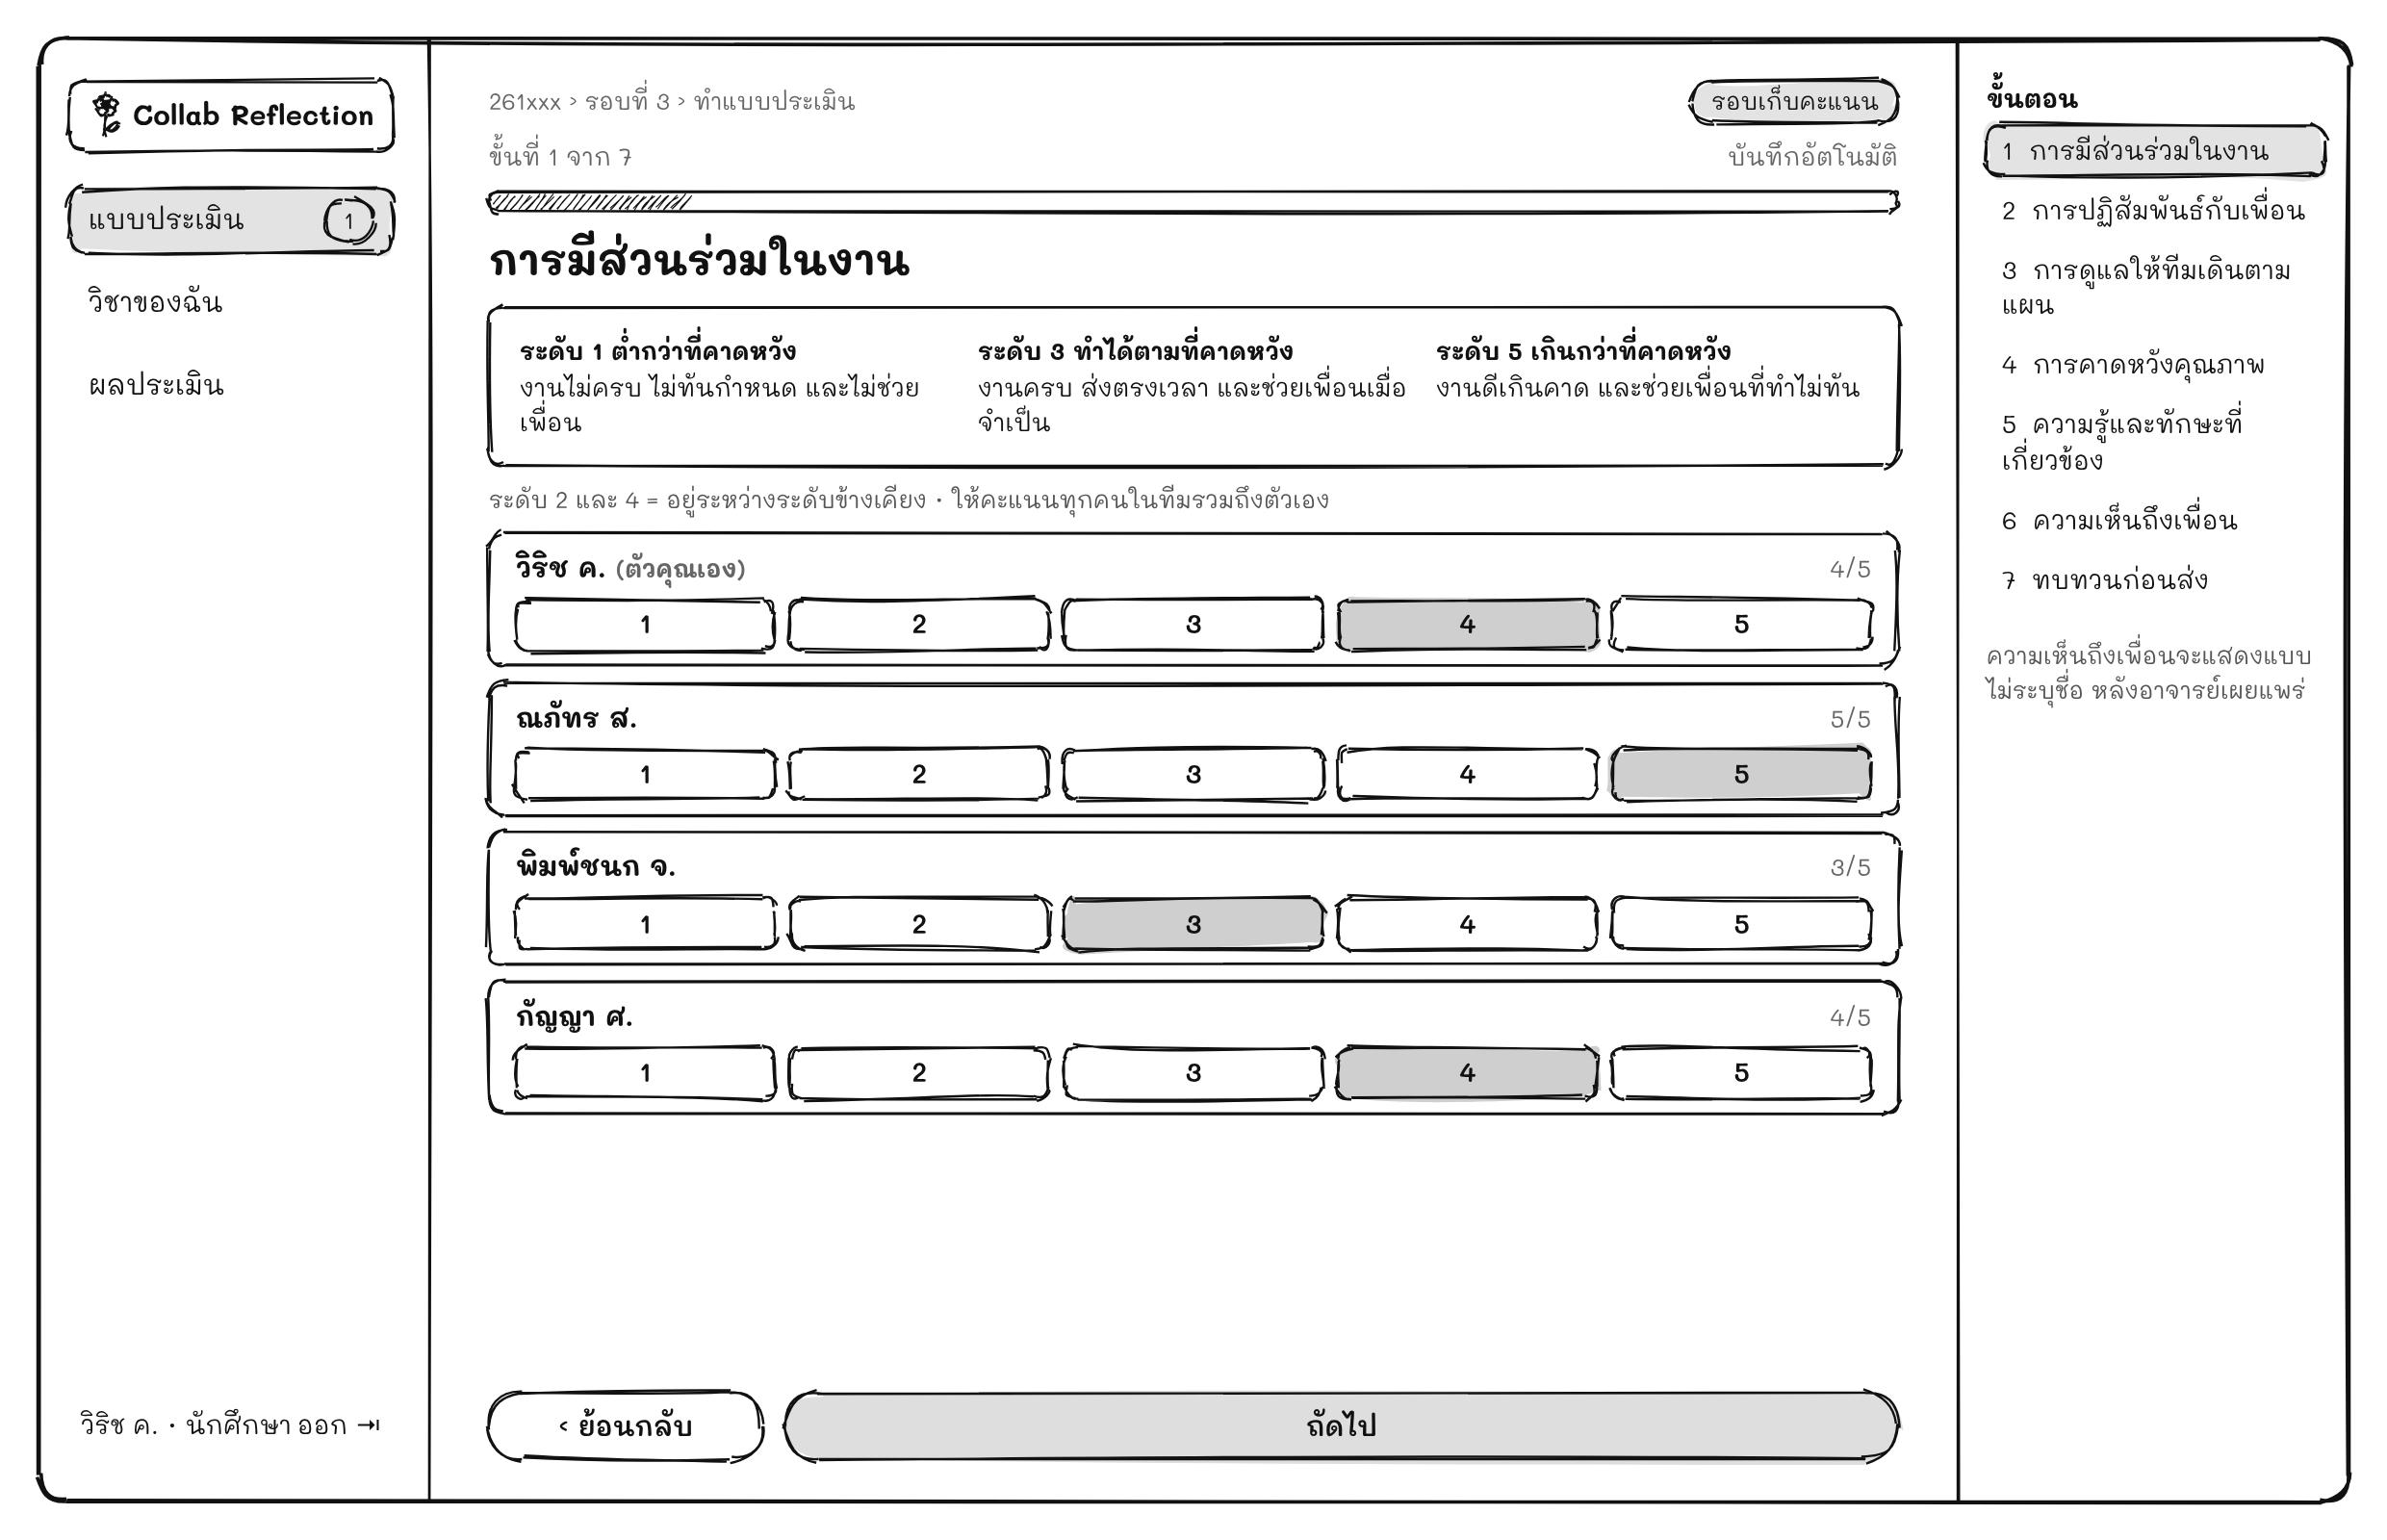
\includegraphics[width=0.85\textwidth]{figures/ch3/fig3-8-student-rating.png}}{\fbox{\parbox{0.8\textwidth}{\centering\vspace{2cm}[วางไฟล์ figures/ch3/fig3-8-student-rating.png]\vspace{2cm}}}}
\caption{หน้าให้คะแนนรายด้าน}\label{fig:ch3-8}
\end{figure}

ขั้นความเห็นถึงเพื่อนใช้แนวคิด ``ให้ดอกไม้ เติมปุ๋ย'' ดอกไม้คือสิ่งที่เพื่อนทำดีอยู่แล้วและควรได้รับคำชมเพื่อให้เติบโตต่อ ส่วนปุ๋ยเป็นสิ่งที่ช่วยให้เพื่อนเติบโตในงานถัดไป หน้าจอมีกล่องอธิบายพร้อมตัวอย่างการเขียน และภาพประกอบการเติบโตจากต้นอ่อนเป็นดอกไม้ ดังรูปที่~\ref{fig:ch3-9}

\begin{figure}[htbp]
\centering
\IfFileExists{figures/ch3/fig3-9-student-comments.png}{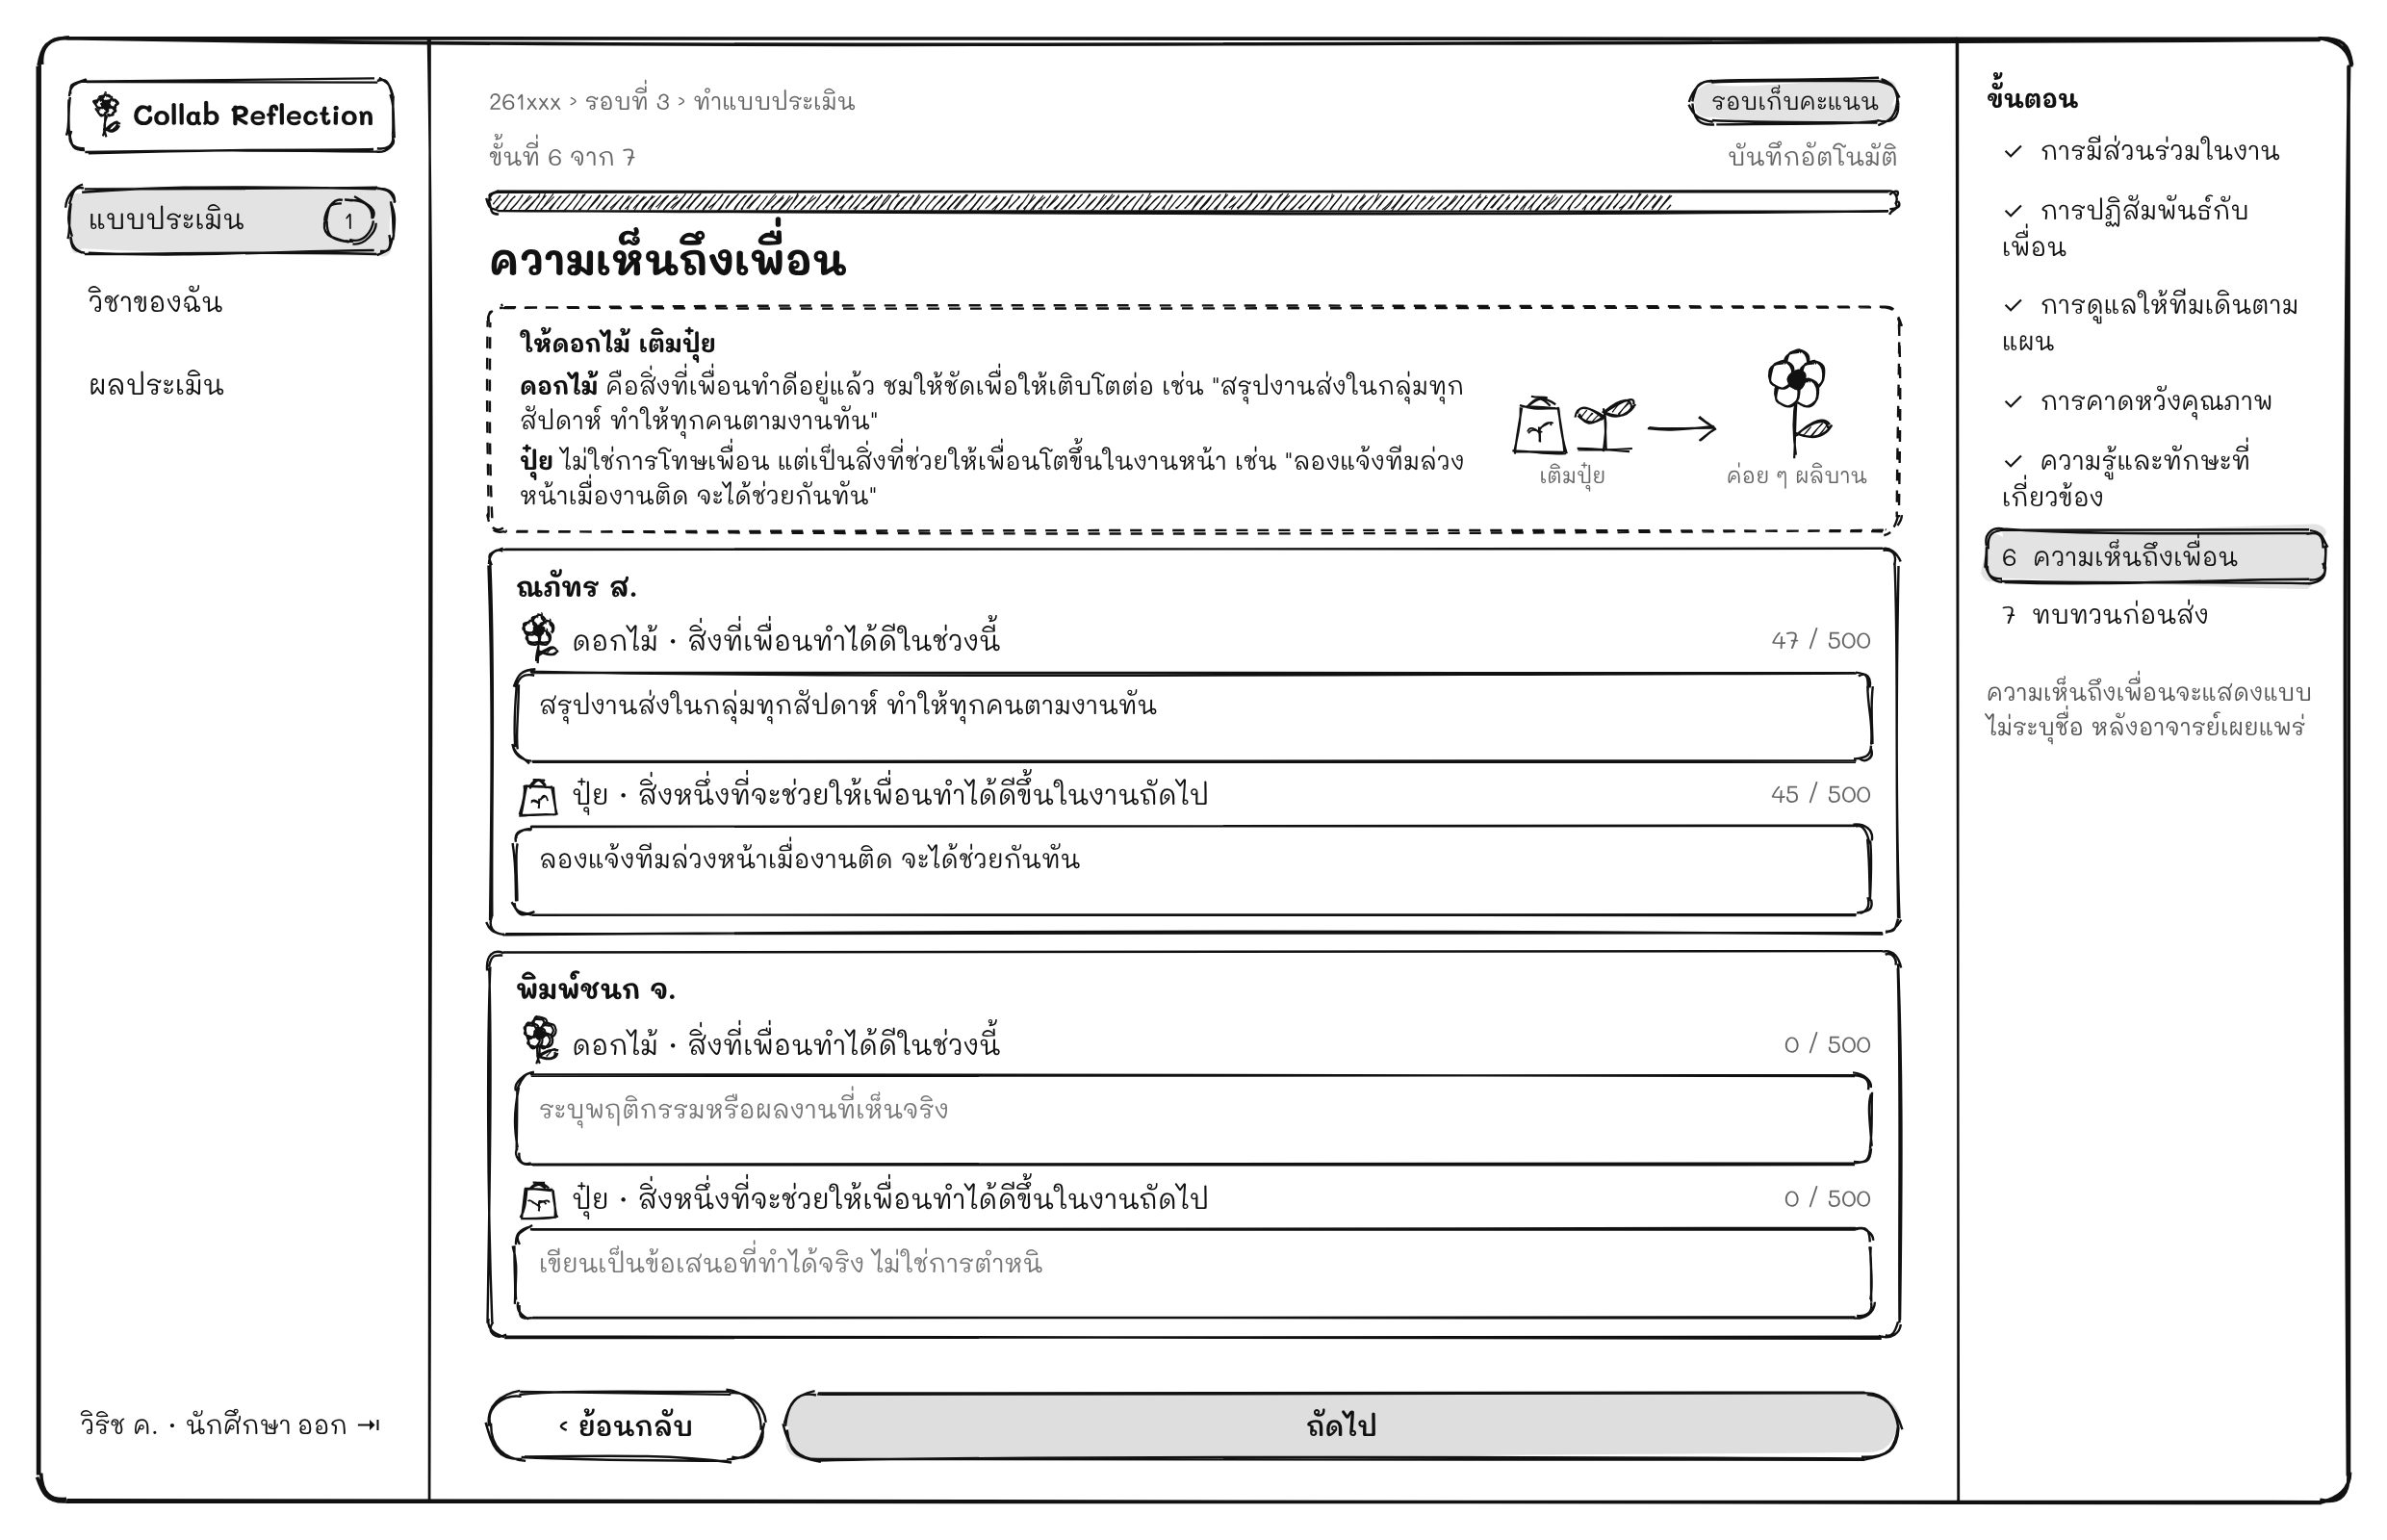
\includegraphics[width=0.85\textwidth]{figures/ch3/fig3-9-student-comments.png}}{\fbox{\parbox{0.8\textwidth}{\centering\vspace{2cm}[วางไฟล์ figures/ch3/fig3-9-student-comments.png]\vspace{2cm}}}}
\caption{หน้าเขียนความเห็นแบบดอกไม้และปุ๋ย}\label{fig:ch3-9}
\end{figure}

หน้าดูผลแสดงคะแนนรายด้านด้วยแผนภูมิเรดาร์ เปรียบเทียบค่าเฉลี่ยที่เพื่อนประเมินกับคะแนนที่ประเมินตนเอง แสดงดอกไม้และปุ๋ยที่ได้รับ ข้อเสนอแนะจากอาจารย์ และมีปุ่มขอความช่วยเหลือสำหรับนักศึกษาที่รู้สึกไม่สบายใจ ดังรูปที่~\ref{fig:ch3-10}

\begin{figure}[htbp]
\centering
\IfFileExists{figures/ch3/fig3-10-student-result.png}{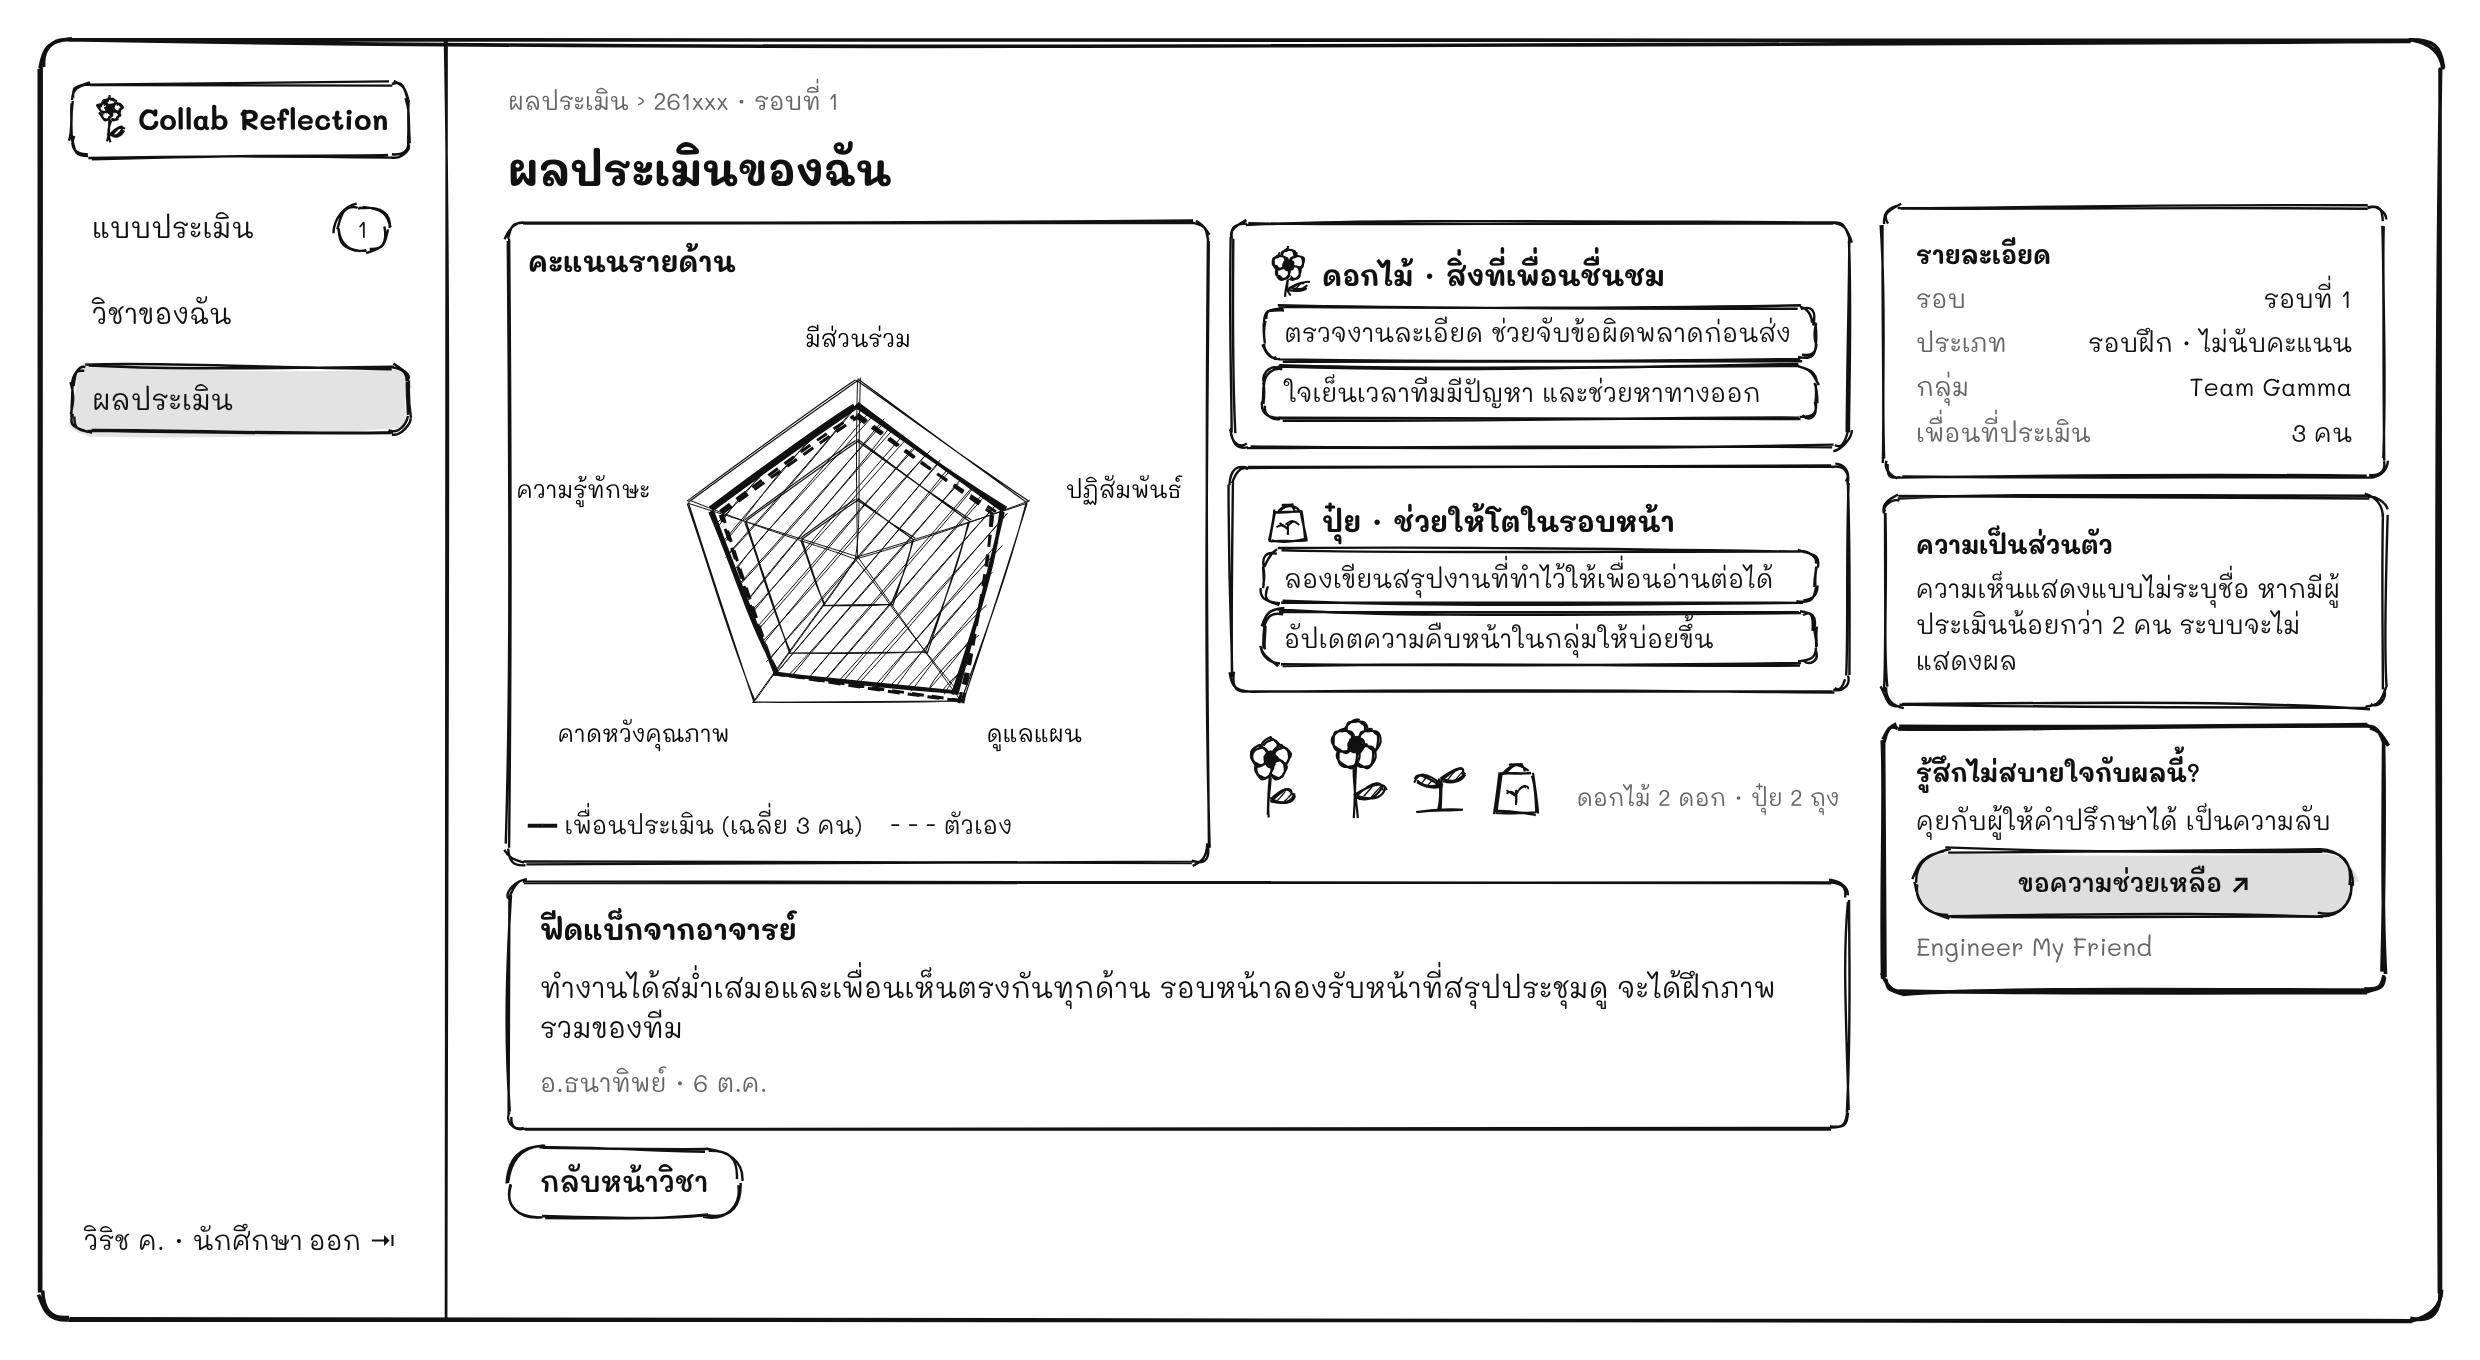
\includegraphics[width=\textwidth]{figures/ch3/fig3-10-student-result.png}}{\fbox{\parbox{0.8\textwidth}{\centering\vspace{2cm}[วางไฟล์ figures/ch3/fig3-10-student-result.png]\vspace{2cm}}}}
\caption{หน้าดูผลการประเมินของนักศึกษา}\label{fig:ch3-10}
\end{figure}

\subsection{หน้าจอฝั่งอาจารย์}\label{sec:3.8.3}

หน้าสมาชิกใช้นำเข้ารายชื่อนักศึกษาจากไฟล์ CSV จัดกลุ่ม และตรวจว่านักศึกษาคนใดยังไม่ยอมรับข้อตกลง PDPA ดังรูปที่~\ref{fig:ch3-11}

\begin{figure}[htbp]
\centering
\IfFileExists{figures/ch3/fig3-11-instructor-members.png}{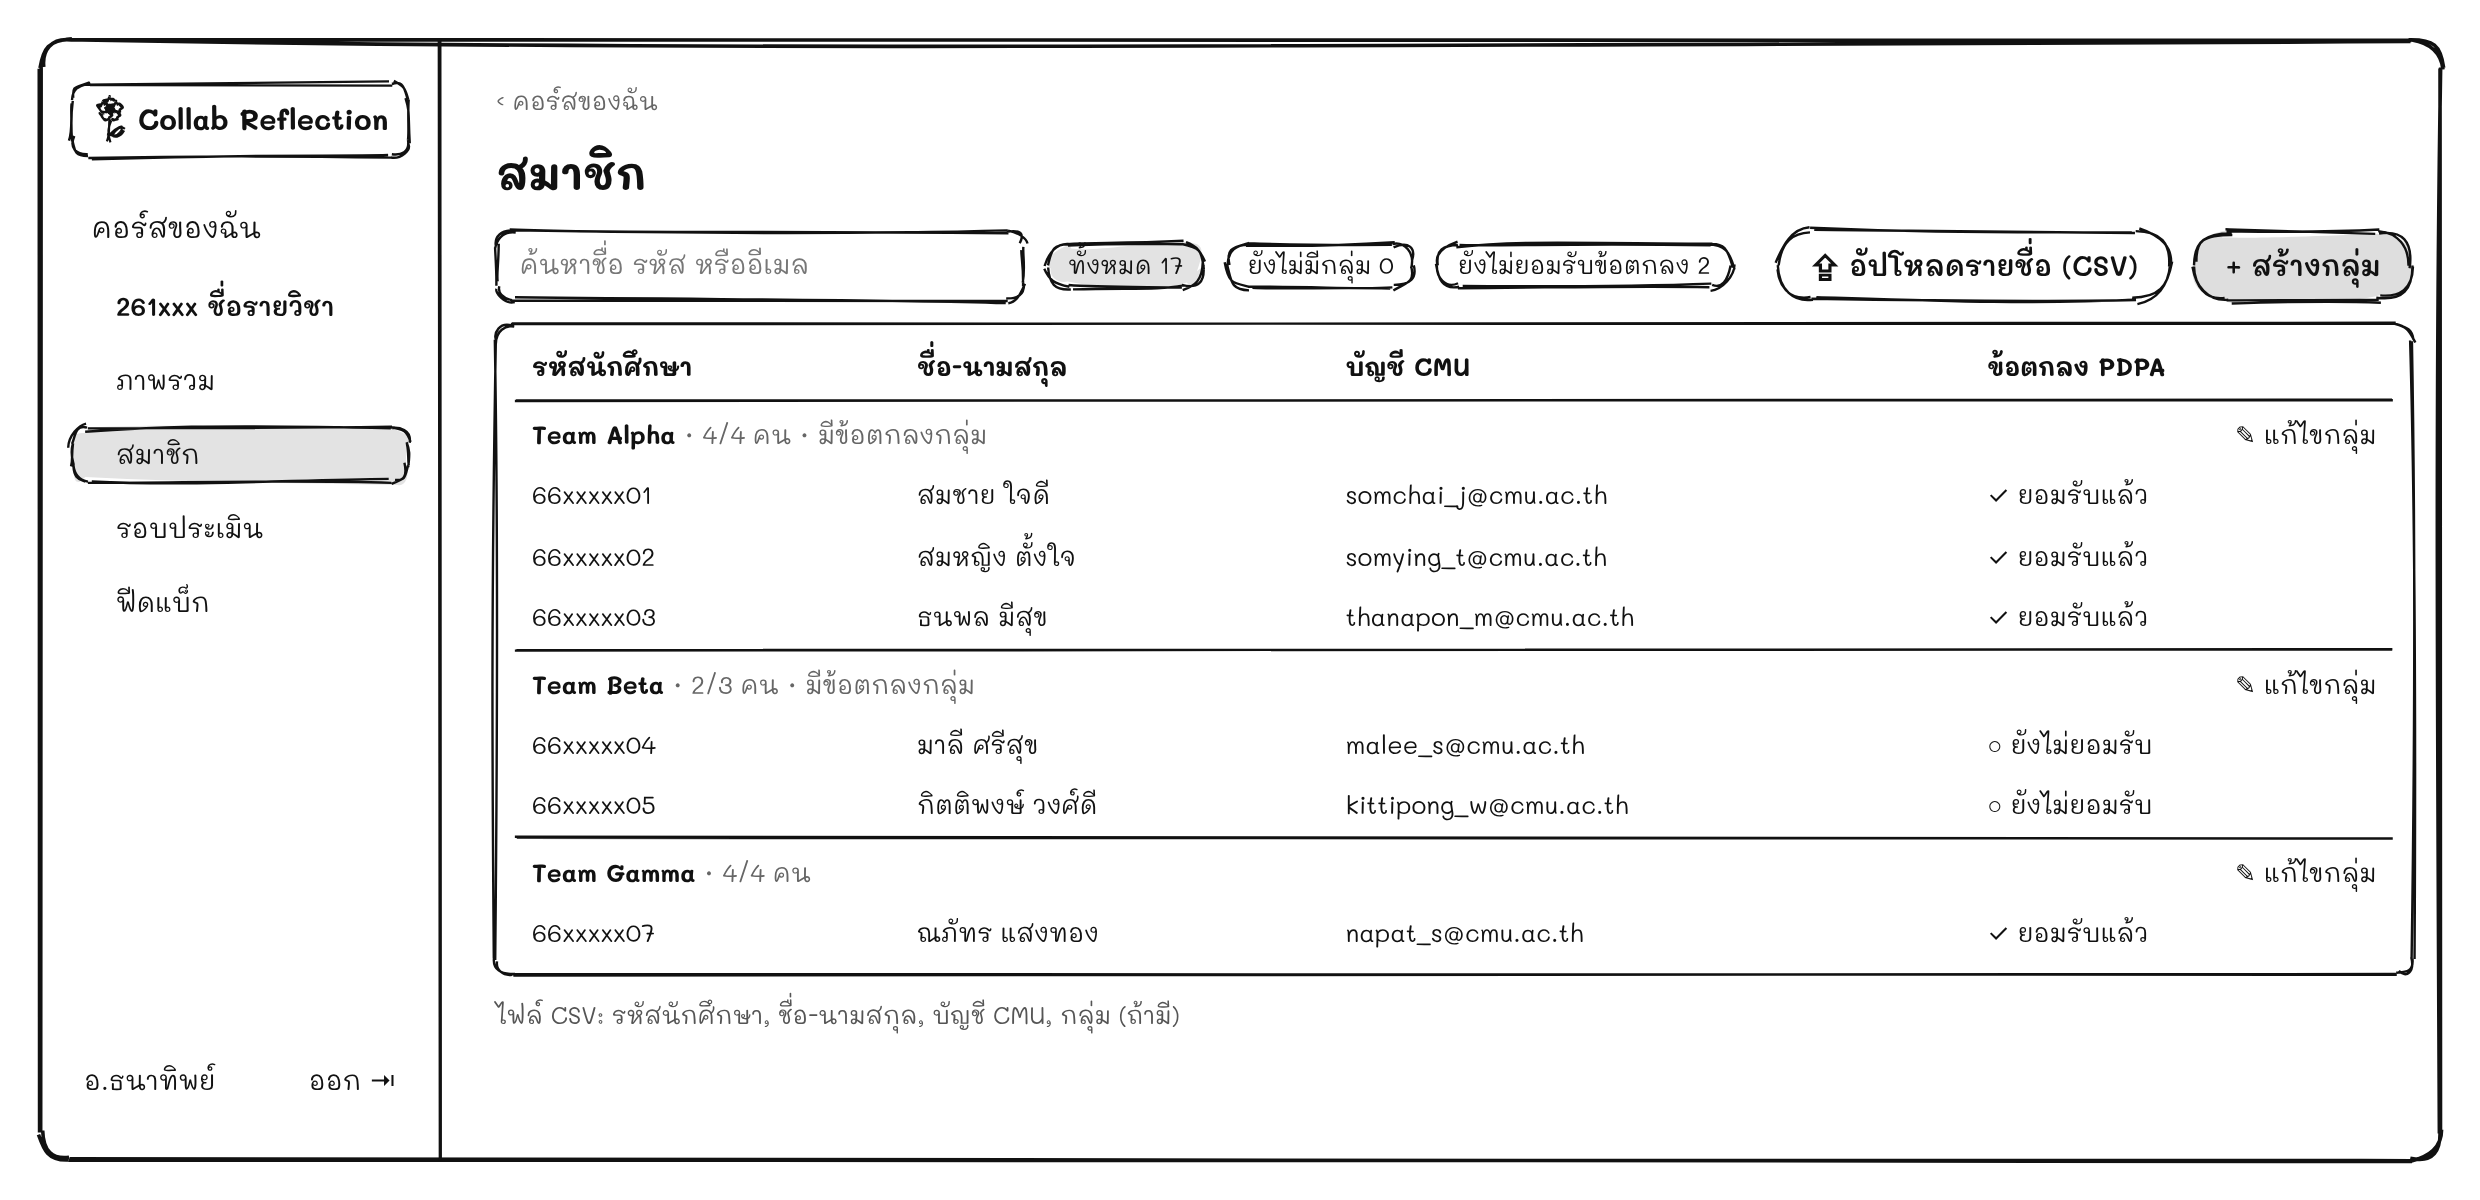
\includegraphics[width=\textwidth]{figures/ch3/fig3-11-instructor-members.png}}{\fbox{\parbox{0.8\textwidth}{\centering\vspace{2cm}[วางไฟล์ figures/ch3/fig3-11-instructor-members.png]\vspace{2cm}}}}
\caption{หน้าจัดการสมาชิกและกลุ่ม}\label{fig:ch3-11}
\end{figure}

หน้ารอบประเมินแสดงรอบทั้งหมดของรายวิชา เมื่อเพิ่มรอบใหม่ อาจารย์ต้องเลือกประเภทของรอบ (รอบฝึกหรือรอบเก็บคะแนน) และกำหนดช่วงเวลาเปิดปิด ดังรูปที่~\ref{fig:ch3-12}

\begin{figure}[htbp]
\centering
\IfFileExists{figures/ch3/fig3-12-instructor-rounds.png}{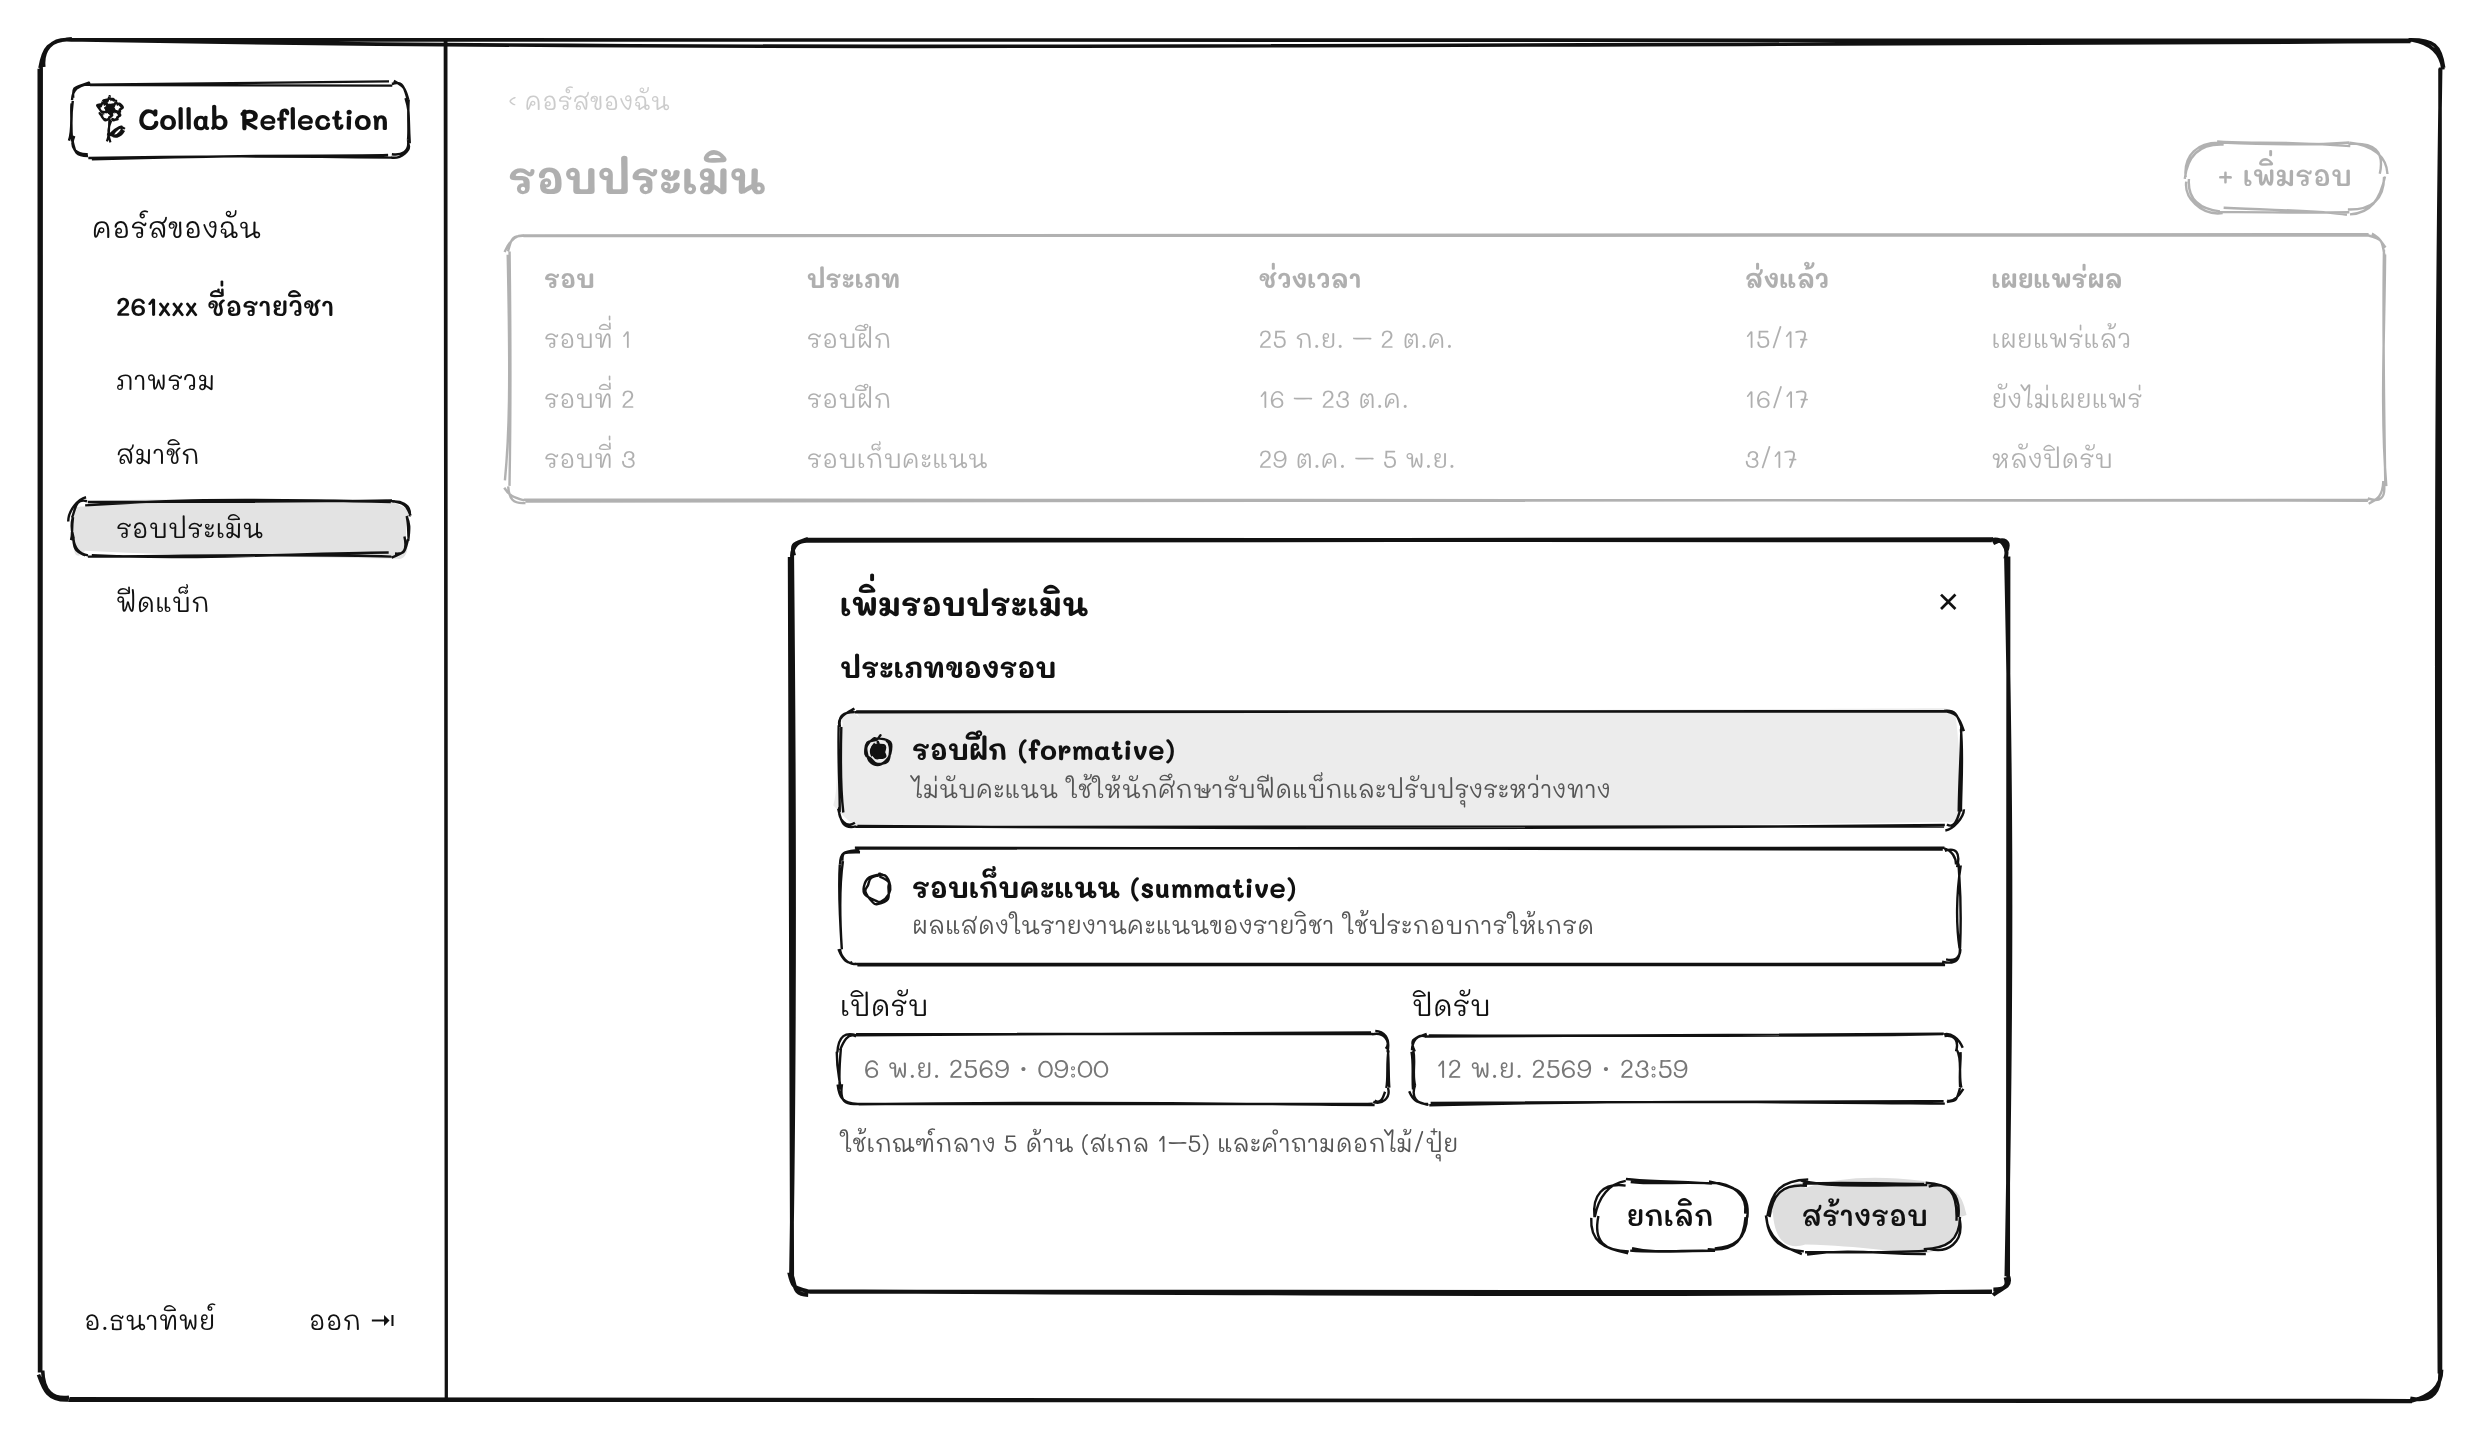
\includegraphics[width=\textwidth]{figures/ch3/fig3-12-instructor-rounds.png}}{\fbox{\parbox{0.8\textwidth}{\centering\vspace{2cm}[วางไฟล์ figures/ch3/fig3-12-instructor-rounds.png]\vspace{2cm}}}}
\caption{หน้าเพิ่มรอบประเมิน}\label{fig:ch3-12}
\end{figure}

แดชบอร์ดแสดงภาพรวมของรอบที่เลือก จำนวนผู้ส่ง แผนภาพเปรียบเทียบคะแนนที่ประเมินตนเองกับที่เพื่อนประเมิน และสัญญาณที่ควรดูของแต่ละทีม ดังรูปที่~\ref{fig:ch3-13}

\begin{figure}[htbp]
\centering
\IfFileExists{figures/ch3/fig3-13-instructor-overview.png}{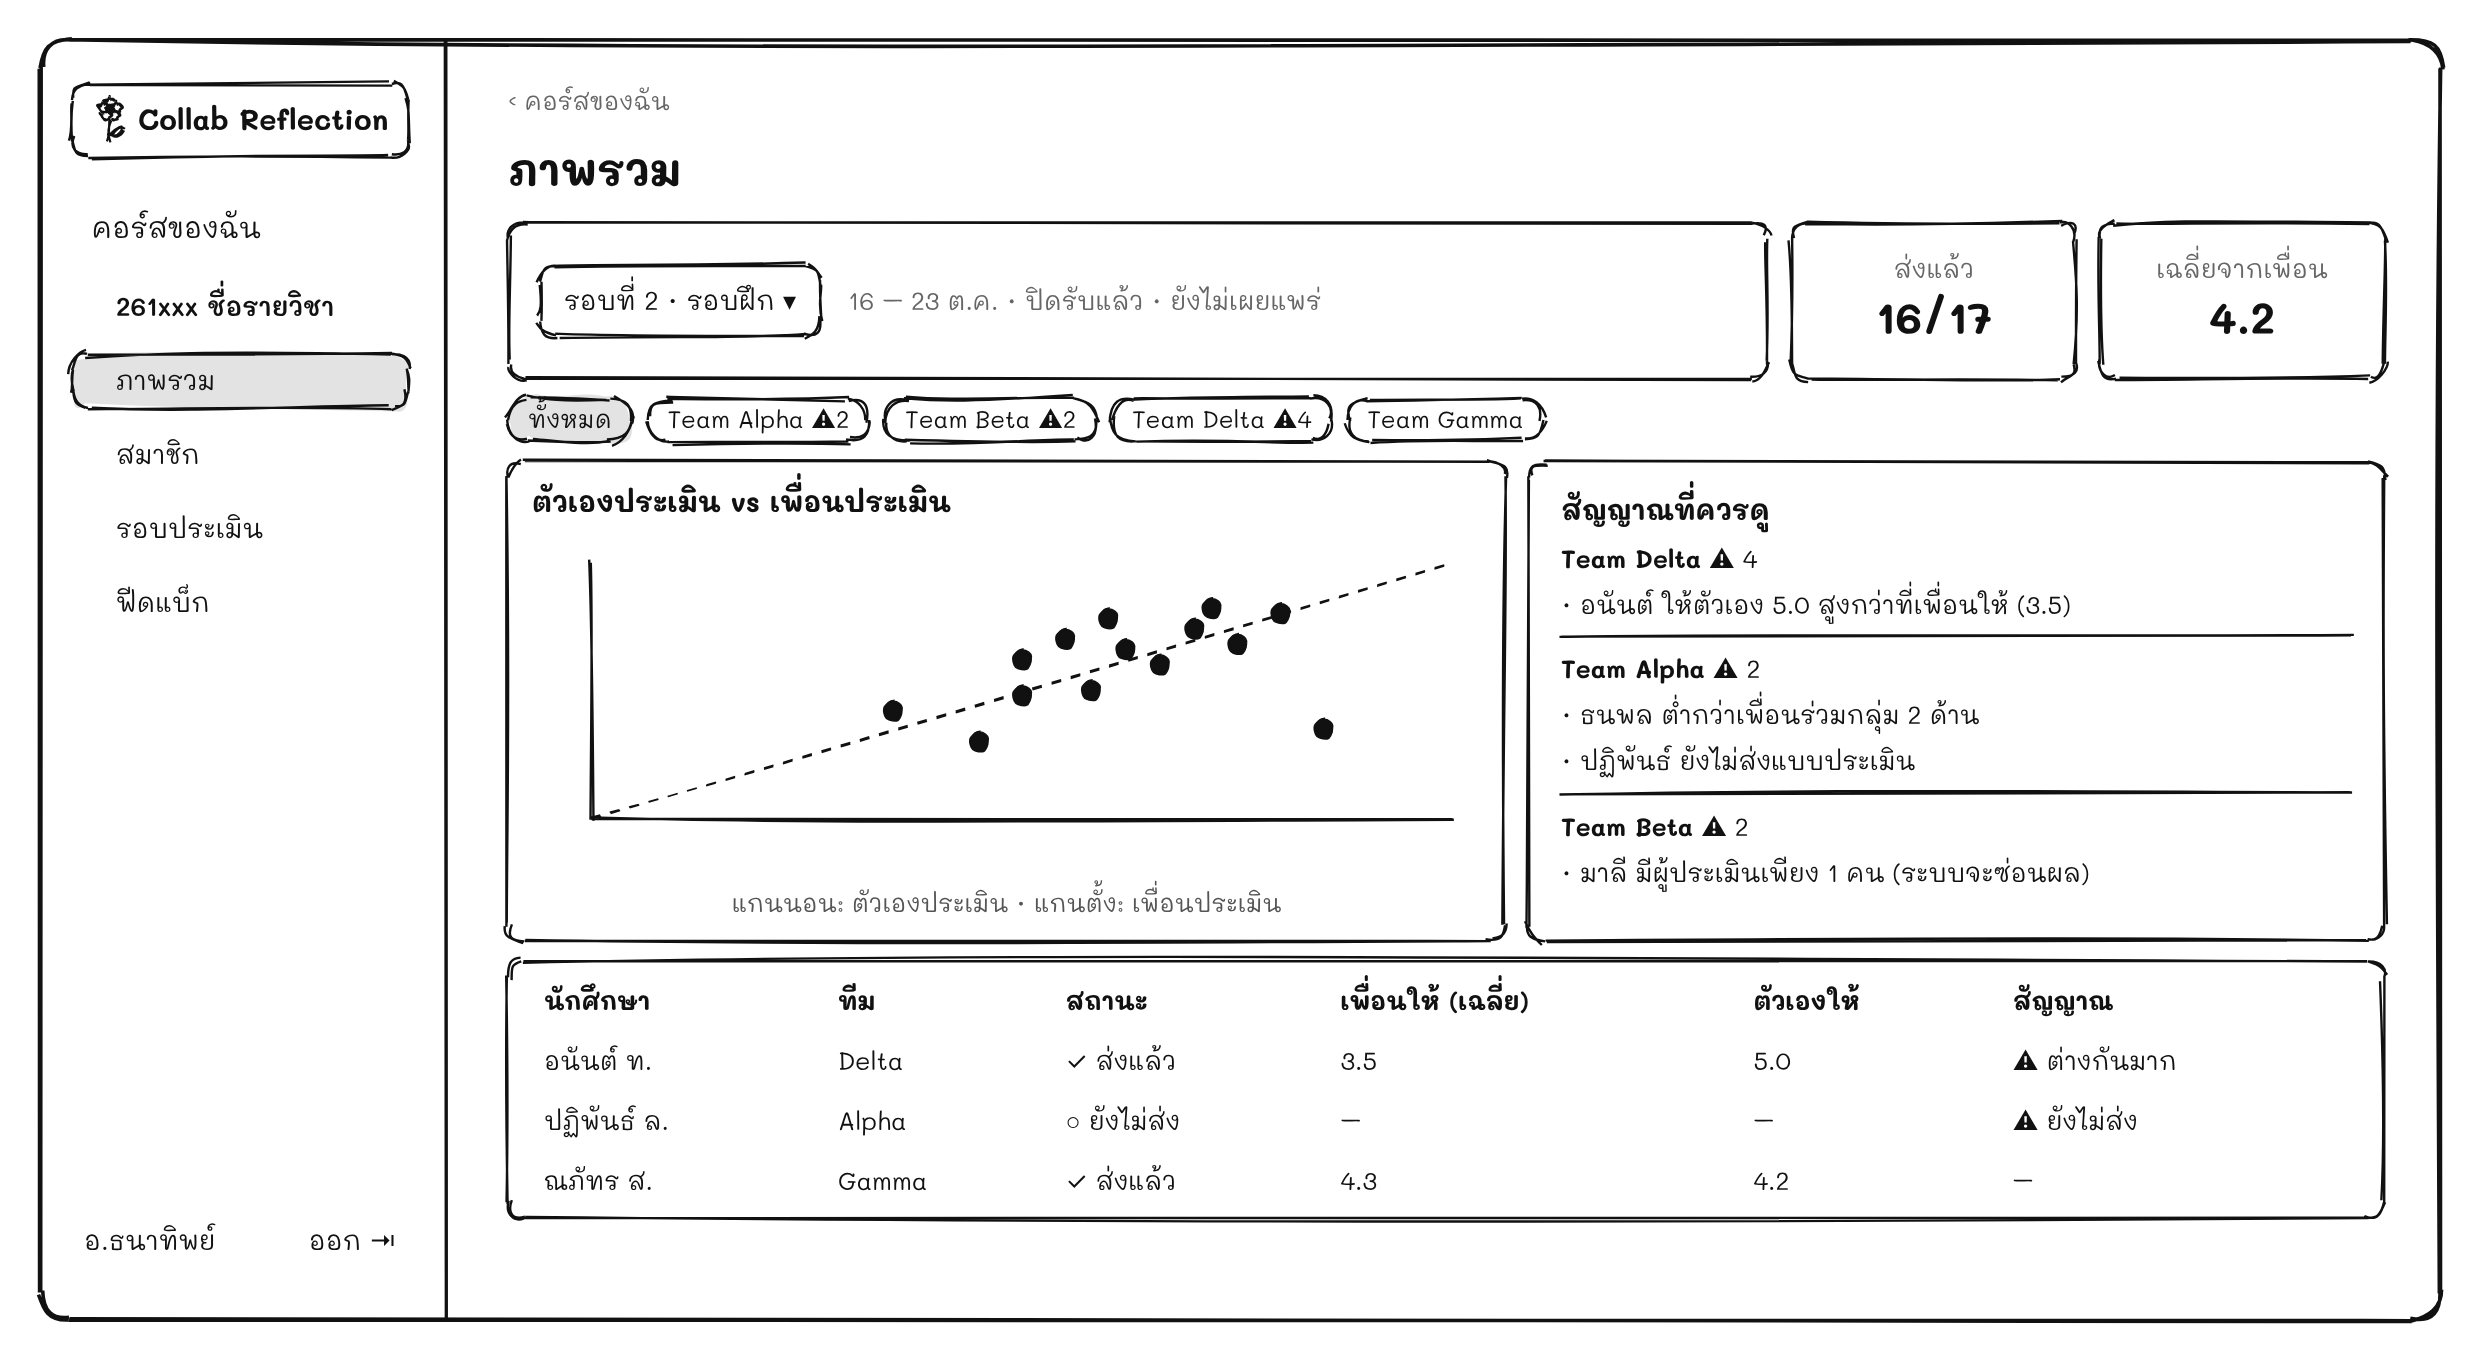
\includegraphics[width=\textwidth]{figures/ch3/fig3-13-instructor-overview.png}}{\fbox{\parbox{0.8\textwidth}{\centering\vspace{2cm}[วางไฟล์ figures/ch3/fig3-13-instructor-overview.png]\vspace{2cm}}}}
\caption{แดชบอร์ดของอาจารย์}\label{fig:ch3-13}
\end{figure}

หน้าภาพรวมแสดงผลของนักศึกษาทีละคน ให้อาจารย์อ่านดอกไม้และปุ๋ยจากเพื่อน เลือกว่านักศึกษาจะเห็นความเห็นของเพื่อนตามจริงหรือเฉพาะข้อสรุปของอาจารย์ เขียนข้อเสนอแนะ และกดเผยแพร่ผลของทั้งรอบ ดังรูปที่~\ref{fig:ch3-14}

\begin{figure}[htbp]
\centering
\IfFileExists{figures/ch3/fig3-14-instructor-feedback.png}{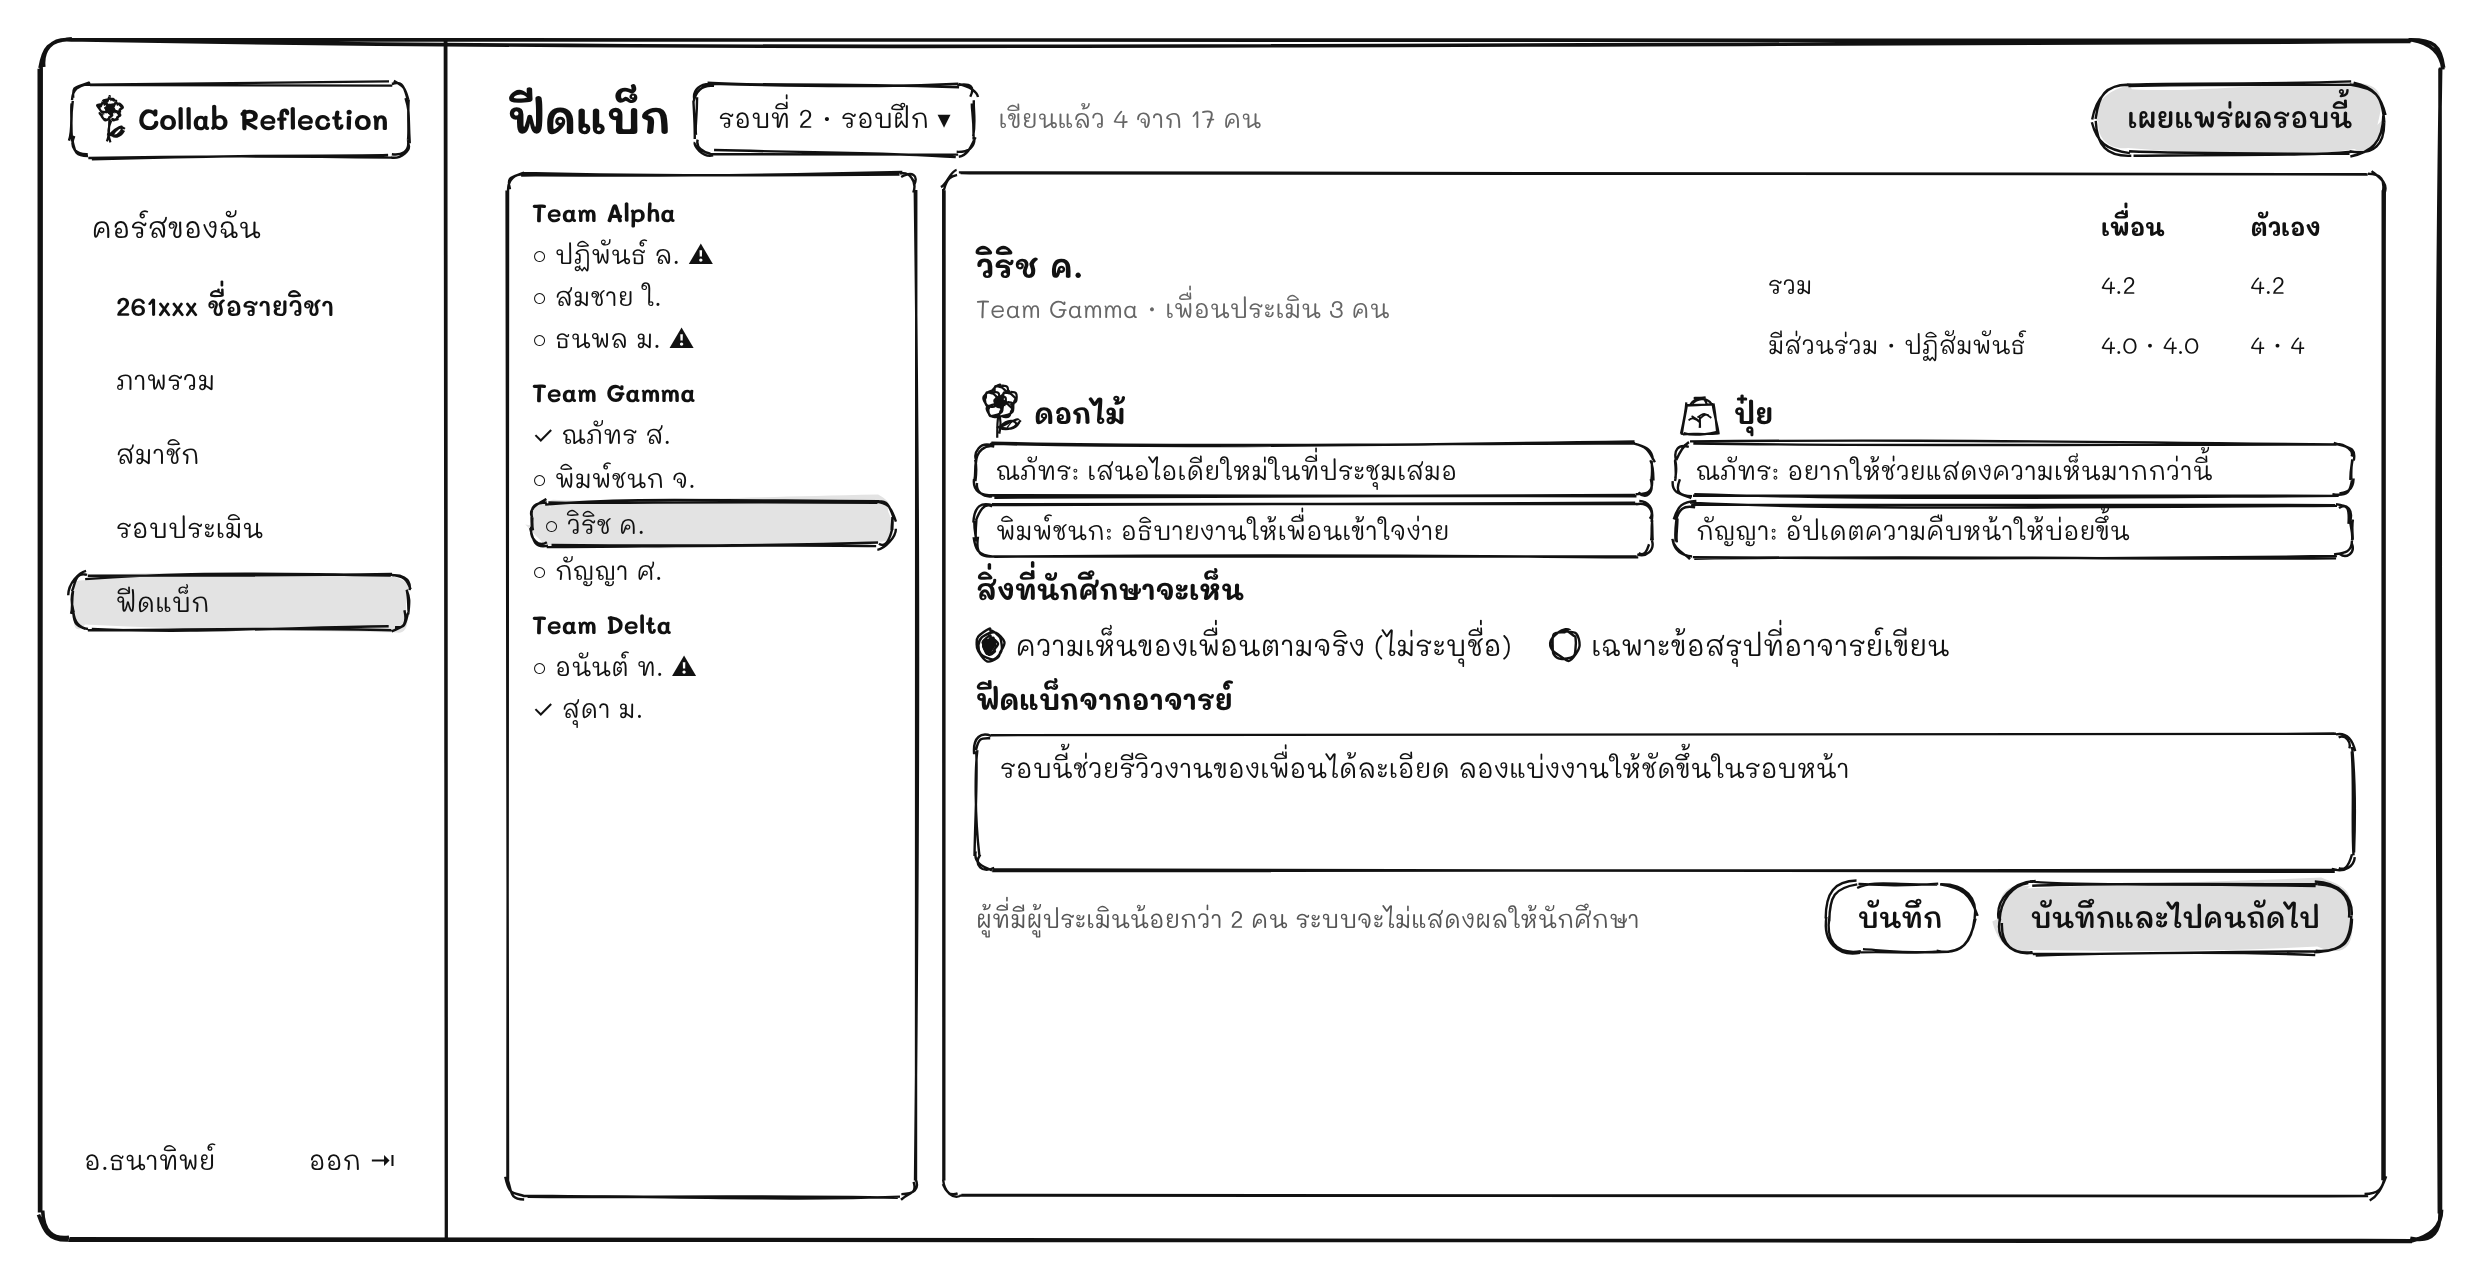
\includegraphics[width=\textwidth]{figures/ch3/fig3-14-instructor-feedback.png}}{\fbox{\parbox{0.8\textwidth}{\centering\vspace{2cm}[วางไฟล์ figures/ch3/fig3-14-instructor-feedback.png]\vspace{2cm}}}}
\caption{หน้าตรวจทานและเผยแพร่ผล}\label{fig:ch3-14}
\end{figure}

\section{ความปลอดภัยและการคุ้มครองข้อมูลส่วนบุคคล}\label{sec:3.9}

\subsection{ความปลอดภัยของระบบ}\label{sec:3.9.1}

\begin{itemize}
  \item เข้าสู่ระบบด้วยบัญชี CMU เท่านั้น และระบบไม่เก็บรหัสผ่าน
  \item ตรวจสิทธิ์ตามบทบาทในทุก API และบังคับกฎการปกปิดตัวตนที่ฝั่งเซิร์ฟเวอร์
  \item เข้ารหัสการสื่อสารด้วย HTTPS และใช้คุกกี้เซสชันแบบ HttpOnly และ Secure
  \item ตรวจสอบข้อมูลขาเข้าทุกครั้ง และใช้ ORM ที่สร้างคำสั่ง SQL แบบมีพารามิเตอร์ เพื่อป้องกัน SQL injection
  \item แบบประเมินที่ส่งแล้วแก้ไขไม่ได้ เพื่อป้องกันการเปลี่ยนคะแนนย้อนหลัง
\end{itemize}

\subsection{การคุ้มครองข้อมูลส่วนบุคคล}\label{sec:3.9.2}

ระบบออกแบบตามหลักของพระราชบัญญัติคุ้มครองข้อมูลส่วนบุคคล พ.ศ. 2562~\cite{pdpa2562} ได้แก่ เก็บข้อมูลเท่าที่จำเป็นต่อการประเมินงานกลุ่มเท่านั้น แจ้งก่อนใช้ว่าเก็บข้อมูลอะไร ใครเห็น และเก็บนานเท่าใด และให้เจ้าของข้อมูลใช้สิทธิ์ขอดู แก้ไข หรือลบข้อมูลได้

เพื่อไม่ให้นักศึกษาที่ไม่ยินยอมบางเรื่องต้องหลุดออกจากระบบจนเก็บคะแนนไม่ได้ ข้อตกลงจึงแบ่งเป็นส่วนจำเป็นและส่วนทางเลือก ดังตารางที่~\ref{tab:ch3-9} ทั้งนี้ คณะผู้จัดทำจะยืนยันระยะเวลาเก็บข้อมูลและฐานทางกฎหมายของการประมวลผลส่วนจำเป็นกับหน่วยงานที่ดูแลการคุ้มครองข้อมูลส่วนบุคคลของมหาวิทยาลัยก่อนใช้งานจริง

\begin{xltabular}{\textwidth}{|P{0.14\textwidth}|Y|Y|}
\caption{การแบ่งข้อตกลงการใช้ข้อมูลส่วนบุคคล}\label{tab:ch3-9}\\
\hline \textbf{ส่วน} & \textbf{ข้อมูลและการใช้งาน} & \textbf{หากไม่ยินยอม} \\ \hline
\endfirsthead
\multicolumn{3}{r}{\small (ต่อ)}\\ \hline \textbf{ส่วน} & \textbf{ข้อมูลและการใช้งาน} & \textbf{หากไม่ยินยอม} \\ \hline
\endhead
ส่วนจำเป็น & ข้อมูลบัญชี CMU รายวิชาและกลุ่มที่สังกัด คะแนนและความเห็นที่ใช้ในการประเมินของรายวิชา & ต้องรับทราบจึงจะใช้ระบบได้ เพราะเป็นข้อมูลขั้นต่ำของการประเมิน \\ \hline
ส่วนทางเลือก 1 & ส่งข้อความที่เขียนให้ปัญญาประดิษฐ์ (AI) ประมวลผล (เฟสที่ 2) & ใช้ระบบและได้คะแนนตามปกติ แต่ข้อความของผู้นั้นจะไม่ถูกส่งให้ปัญญาประดิษฐ์ (AI) \\ \hline
ส่วนทางเลือก 2 & นำข้อมูลแบบไม่ระบุตัวตนไปใช้พัฒนาระบบและในงานวิจัย & ใช้ระบบและได้คะแนนตามปกติ แต่ข้อมูลของผู้นั้นจะไม่ถูกนำไปใช้ \\ \hline
\end{xltabular}

\subsection{การดูแลความรู้สึกของผู้ใช้}\label{sec:3.9.3}

ข้อเสนอแนะจากเพื่อนอาจกระทบความรู้สึกของผู้รับได้แม้ผ่านการกลั่นกรองแล้ว ระบบจึงลดโอกาสเกิดความคิดเห็นที่ทำร้ายจิตใจตั้งแต่ต้นทาง ด้วยคำถามแบบดอกไม้และปุ๋ย คำแนะนำการเขียน และการตรวจทานของอาจารย์ก่อนเผยแพร่ และที่หน้าดูผลมีปุ่มขอความช่วยเหลือที่เชื่อมไปยังช่องทางให้คำปรึกษา เช่น โครงการ Entaneer Mind Friend สำหรับนักศึกษาที่รู้สึกไม่สบายใจ

\section{แผนการประเมินระบบและตัวชี้วัดความสำเร็จ}\label{sec:3.10}

การประเมินระบบอยู่ในระยะที่ 4 ของการดำเนินงาน แบ่งเป็นการตรวจสอบว่าระบบทำงานถูกต้องตามที่ออกแบบ (verification) และการยืนยันว่าระบบแก้ปัญหาของผู้ใช้ได้จริง (validation)

\subsection{การตรวจสอบความถูกต้องของระบบ}\label{sec:3.10.1}

\begin{itemize}
  \item Unit test ด้วย Vitest สำหรับตรรกะสำคัญ เช่น การคำนวณค่าเฉลี่ยรายด้าน เงื่อนไขซ่อนผลเมื่อผู้ประเมินไม่ถึง 2 คน และเงื่อนไขสัญญาณเตือน
  \item Integration test ของ API ทุกเส้นทาง รวมถึงทดสอบว่านักศึกษาเรียกดูข้อมูลที่ตนไม่มีสิทธิ์ไม่ได้
  \item End-to-end test ด้วย Cypress สำหรับขั้นตอนหลัก ได้แก่ นักศึกษาส่งแบบประเมิน และอาจารย์ตรวจทานและเผยแพร่ผล
  \item ทดสอบโหลดด้วยจำนวนผู้ใช้เทียบเท่าหนึ่งรายวิชา
  \item ส่วน AI (เฟสที่ 2): วัดความสอดคล้องระหว่างผลการตรวจโทนของโมเดลกับการติดป้ายกำกับโดยคน บนชุดข้อความภาษาไทยตัวอย่าง
\end{itemize}

\subsection{การนำร่องใช้งานจริง}\label{sec:3.10.2}

คณะผู้จัดทำจะนำระบบไปทดลองใช้ในรายวิชาที่มีการทำงานกลุ่มระยะยาวของภาควิชาวิศวกรรมคอมพิวเตอร์อย่างน้อย 1 รายวิชา โดยมีรอบฝึกอย่างน้อย 1 รอบและรอบเก็บคะแนน 1 รอบ หลังใช้งานจะเก็บแบบสอบถาม System Usability Scale (SUS)~\cite{brooke1996sus} จากทั้งอาจารย์และนักศึกษา และสัมภาษณ์อาจารย์ผู้สอนเรื่องภาระงานและประโยชน์ที่ได้รับ เพื่อนำไปพัฒนาในระยะถัดไป

\subsection{ตัวชี้วัดความสำเร็จ}\label{sec:3.10.3}

ตัวชี้วัดความสำเร็จของโครงงานแสดงในตารางที่~\ref{tab:ch3-10}

\begin{xltabular}{\textwidth}{|P{0.14\textwidth}|P{0.2\textwidth}|Y|P{0.15\textwidth}|}
\caption{ตัวชี้วัดความสำเร็จของโครงงาน}\label{tab:ch3-10}\\
\hline \textbf{ด้าน} & \textbf{ตัวชี้วัด} & \textbf{เป้าหมาย} & \textbf{วิธีวัด} \\ \hline
\endfirsthead
\multicolumn{4}{r}{\small (ต่อ)}\\ \hline \textbf{ด้าน} & \textbf{ตัวชี้วัด} & \textbf{เป้าหมาย} & \textbf{วิธีวัด} \\ \hline
\endhead
ความถูกต้องของระบบ & กรณีทดสอบของฟีเจอร์ระยะที่ 1 & ผ่านทั้งหมด & Vitest และ Cypress \\ \hline
การใช้งานจริง & จำนวนรายวิชานำร่อง & อย่างน้อย 1 รายวิชา และ 2 รอบประเมิน & บันทึกการใช้งานในระบบ \\ \hline
การรองรับผู้ใช้ & จำนวนผู้ใช้ที่ใช้งานพร้อมกันได้ & ประมาณ 90 คนต่อรายวิชา ตามสัดส่วนนักศึกษาต่ออาจารย์ในรายวิชาเป้าหมาย & ทดสอบโหลด \\ \hline
การมีส่วนร่วม & อัตราการส่งแบบประเมินต่อรอบ & อย่างน้อยร้อยละ 80 & ข้อมูลในระบบ \\ \hline
ความง่ายในการใช้งาน & คะแนน SUS & อย่างน้อย 68 คะแนน ซึ่งเป็นค่าเฉลี่ยอ้างอิงทั่วไป~\cite{sauro2011sus} ทั้งฝั่งอาจารย์และนักศึกษา & แบบสอบถาม SUS \\ \hline
ภาระงานของอาจารย์ & เวลาที่ใช้ตรวจทานและเผยแพร่ผลต่อหนึ่งกลุ่ม & น้อยกว่าวิธีเดิมที่อาจารย์ใช้อยู่ & จับเวลาและสัมภาษณ์อาจารย์ \\ \hline
คุณภาพฟีดแบ็ก & สัดส่วนความเห็นที่ระบุพฤติกรรมและเสนอสิ่งที่ทำได้จริง & รอบเก็บคะแนนสูงกว่ารอบฝึกรอบแรก & จัดหมวดความเห็นโดยผู้ประเมิน 2 คน \\ \hline
\end{xltabular}



\bibliography{sampleReport}

\ifproject
\normalspacing
\appendix
% ภาคผนวก ก — วางหลัง \appendix ใน sampleReport.tex (หรือรวมเข้า chapters/appendix.tex)
\chapter{คำถามที่ใช้ในการสัมภาษณ์อาจารย์ผู้สอน}\label{app:interview}

ภาคผนวกนี้แสดงคำถามที่ใช้ในการสัมภาษณ์อาจารย์ผู้สอน 5 ท่าน (หัวข้อ~\ref{sec:3.2}) แบ่งเป็นคำถามหลักและคำถามเพิ่มเติม

\section{คำถามหลัก}
\begin{enumerate}
  \item ที่ผ่านมาตอนให้นักศึกษาทำงานกลุ่ม อาจารย์เจอปัญหาใดบ้างที่รู้สึกว่าแก้ยาก
  \item อาจารย์รู้ได้อย่างไรว่าใครในกลุ่มทำงานมาก-น้อย หรือมีปัญหาความขัดแย้งกันภายในกลุ่ม
  \item เคยมีกรณีที่นักศึกษาบางคน ``โหน'' งานกลุ่ม (free-rider) หรือไม่ ถ้าหากมีแล้วอาจารย์จัดการอย่างไร
  \item เคยใช้เครื่องมือหรือวิธีอะไรในการประเมิน peer review บ้าง (แบบฟอร์มกระดาษ, Google Form, ระบบของมหาลัย ฯลฯ)
  \item เครื่องมือที่เคยใช้ มีจุดไหนที่ใช้ยาก ไม่สะดวก หรือข้อมูลที่ได้ไม่ตรงกับสิ่งที่ต้องการ
  \item ในบรรดาที่เคยใช้ เครื่องมือใดที่อาจารย์รู้สึกว่าดีที่สุด เพราะอะไร
  \item เวลาให้คะแนน peer evaluation อาจารย์ดูจากปัจจัยใดเป็นหลัก (คะแนนตัวเลข, comment, สัดส่วนงาน)
  \item ถ้ามีระบบ dashboard ให้อาจารย์เห็นภาพรวมกลุ่ม อยากเห็นข้อมูลในรูปแบบใดมากที่สุด (กราฟ, timeline, สรุปข้อความ)
  \item อาจารย์คิดว่าความถี่ในการให้นักศึกษาส่ง reflection/peer review ควรเป็นอย่างไร (ทุกสัปดาห์, กลางเทอม, จบโปรเจค)
  \item ถ้ามีปัญญาประดิษฐ์ (AI) ช่วย flag ความขัดแย้งในกลุ่มจากข้อความ reflection อาจารย์คิดว่าควร flag แบบไหนถึงจะมีประโยชน์ต่อผู้ใช้งาน (เช่น คำพูดเชิงลบ, ขาดการตอบสนอง)
  \item อาจารย์กังวลอะไรไหมถ้าปัญญาประดิษฐ์ (AI) ต้องอ่าน/วิเคราะห์ ข้อความของนักศึกษา เช่น เรื่อง privacy หรือความแม่นยำ
  \item ถ้าระบบ flag ผิดพลาด (false positive) อาจารย์อยากจัดการอย่างไร เช่น แจ้งเตือน vs ต้องยืนยันก่อน
\end{enumerate}
\section{คำถามเพิ่มเติม}
\begin{enumerate}
  \item อาจารย์สอน/ดูแลโปรเจคนักศึกษามานานแค่ไหน ส่วนใหญ่เป็นวิชาแบบใด
  \item ปัญหาที่เจอบ่อยที่สุดตอนดูแลนักศึกษาทำโปรเจคหรืองานทีต้องใช้เวลานานๆ คืออะไร
  \item อาจารย์มีวิธีติดตามความคืบหน้าของนักศึกษาระหว่างเทอมอย่างไร
  \item ถ้าจะให้เปลี่ยนมาใช้ระบบ/เครื่องมือใหม่แทนของเดิม อาจารย์กังวลเรื่องอะไรบ้าง (เช่น เสียเวลาเรียนรู้ใหม่, ข้อมูลนักศึกษาไม่ปลอดภัย, ความน่าเชื่อถือของระบบ, ต้องเปลี่ยนวิธีสอน)
\end{enumerate}


%% Display glossary (optional) -- need glossary option.
\ifglossary\glossarypage\fi

%% Display index (optional) -- need idx option.
\ifindex\indexpage\fi

\fi % \ifproject
\end{document}
"
\providecommand\reportmode{semifinal}
\documentclass[\reportmode]{cpecmu}

%% This is a sample document demonstrating how to use the CPECMU
%% project template. If you are having trouble, see "cpecmu.pdf" for
%% documentation.

\projectNo{S006-1}
\acadyear{2026}

%% ชื่อระบบ Collab Reflection เป็นชื่อรอง ใช้ \newline เพราะชื่อโครงงานถูกวางในเซลล์ตารางด้วย
\titleTH{แพลตฟอร์มประเมินตนเองและเพื่อนในกลุ่มเพื่อการพัฒนาตนเอง\newline Collab Reflection}
\titleEN{Self and Peer Evaluation Platform for Personal Development\newline Collab Reflection}

\author{นางสาวดารารัตน์ บัวยิ้ม}{Dararat Buayim}{660610759}
\author{นางสาวบัวชมพู ฤกษ์สุทธิรัตน์}{Buachompoo Rerksuitthirat}{660610768}
\author{นายปฏิพันธ์ เลขนอก}{Patiphan Leknok}{660610771}
\author{นายรัชชานนท์ ไชยวงค์}{Ratchanon Chaiwong}{660610789}

\cpeadvisor{thanatip}
%% ลำดับกรรมการตาม portal: สาลินี อานันท์ พฤษภ์
%% ชื่อภาษาอังกฤษยังไม่ได้ตรวจกับรายชื่อของภาค
\committee{ผศ.ดร.\,สาลินี สันติธีรากุล}{Asst.\,Prof.\,Salinee Santiteerakul, Ph.D.}
\cpecommittee{arnan}
\cpecommittee{pruet}

%% Some possible packages to include:
\usepackage[final]{graphicx} % for including graphics

%% Add bookmarks and hyperlinks in the document.
\PassOptionsToPackage{hyphens}{url}
\usepackage[colorlinks=true,allcolors=Blue4,citecolor=red,linktoc=all]{hyperref}
\def\UrlLeft#1\UrlRight{$#1$}

%% Needed just by this example, but maybe not by most reports
\usepackage{afterpage} % for outputting
\usepackage{pdflscape} % for landscape figures and tables. 
\usepackage{capt-of}   % caption for the plan (Gantt chart) table in chapter 1

%% Column types shared by the tables in chapters 2 and 3
\newcolumntype{Y}{>{\raggedright\arraybackslash}X}
\newcolumntype{P}[1]{>{\raggedright\arraybackslash}p{#1}}

%% Some other useful packages. Look these up to find out how to use
%% them.
% \usepackage{natbib}    % for author-year citation styles
% \usepackage{txfonts}
% \usepackage{appendix}  % for appendices on a per-chapter basis
% \usepackage{xtab}      % for tables that go over multiple pages
% \usepackage{subfigure} % for subfigures within a figure
% \usepackage{pstricks,pdftricks} % for access to special PostScript and PDF commands
% \usepackage{nomencl}   % if you have a list of abbreviations

%% if you're having problems with overfull boxes, you may need to increase
%% the tolerance to 9999
% \tolerance=9999
%% Thai text has few break points; allow extra stretch so lines do not run into the margin
\setlength{\emergencystretch}{2em}

\bibliographystyle{plain}
% \bibliographystyle{IEEEbib}

% \renewcommand{\topfraction}{0.85}
% \renewcommand{\textfraction}{0.1}
% \renewcommand{\floatpagefraction}{0.75}

%% Example for glossary entry
%% Need to use glossary option
%% See glossaries package for complete documentation.
\ifglossary
  \newglossaryentry{lorem ipsum}{
    name=lorem ipsum,
    description={derived from Latin dolorem ipsum, translated as ``pain itself''}
  }
\fi

%% Uncomment this command to preview only specified LaTeX file(s)
%% imported with \include command below.
%% Any other file imported via \include but not specified here will not
%% be previewed.
%% Useful if your report is large, as you might not want to build
%% the entire file when editing a certain part of your report.
% \includeonly{chapters/intro,chapters/background}

\begin{document}
\maketitle
\makesignature

\ifproject
\begin{abstractTH}
Peer review คือการประเมินตนเองและประเมินเพื่อนในกลุ่ม ซึ่งเป็นกระบวนการสะท้อนคิดที่ช่วยให้ผู้เรียนเห็นจุดแข็งและจุดที่ควรพัฒนาของตนเอง ผ่านข้อเสนอแนะจากตนเอง เพื่อนร่วมกลุ่ม และอาจารย์ผู้สอน โดยการให้ข้อเสนอแนะเป็นกลไกสำคัญที่ผู้เรียนนำไปใช้พัฒนาการเรียนรู้และการทำงานร่วมกับผู้อื่นของตนเอง

ในปัจจุบัน การให้ข้อเสนอแนะในรายวิชาที่มีนักศึกษาจำนวนมากและมีการทำงานกลุ่มนั้นมีความยุ่งยาก เนื่องจากอาจารย์ผู้สอน (Instructor) ต้องอ่านผลประเมินทั้งหมด คัดแยกประเด็น และเขียนข้อเสนอแนะเฉพาะบุคคลให้นักศึกษาแต่ละคน ซึ่งเป็นภาระที่ใช้เวลามากและทำให้ไม่สามารถให้ข้อเสนอแนะได้อย่างทั่วถึง นอกจากนี้ ถ้อยคำในการประเมินเพื่อนบางครั้งอาจไม่เหมาะสม ทำให้ผู้รับข้อเสนอแนะไม่สามารถนำไปพัฒนาตนเองได้อย่างเต็มที่

คณะผู้จัดทำจึงได้จัดทำโครงงานเพื่อพัฒนาเว็บแอปพลิเคชัน Collab Reflection ที่ผสานเทคโนโลยีปัญญาประดิษฐ์ (AI) เข้า กับ Web Application ซึ่งสามารถให้นักศึกษาประเมินตนเองและประเมินเพื่อนในกลุ่มได้ และสามารถให้อาจารย์ดูผลการประเมินที่ถูกจำแนกประเภทผ่านแดชบอร์ดได้ โดยระบบในระยะที่ 1 ประกอบด้วย แบบประเมินตนเอง แบบประเมินเพื่อนในกลุ่ม และแดชบอร์ดสำหรับอาจารย์ ส่วนระยะที่ 2 จะเพิ่มระบบ AI ที่ช่วยตรวจโทนข้อความและเสนอถ้อยคำเชิงสร้างสรรค์ให้ผู้เขียนเลือกใช้ รวมถึง AI ที่สรุปผลเพื่อช่วยอาจารย์ร่างข้อเสนอแนะตอบกลับนักศึกษา โดยอาจารย์ยังเป็นผู้ตรวจทานก่อนส่งทุกครั้ง
\end{abstractTH}

\begin{abstract}
Peer review is a process of self-assessment and peer assessment within a group. It is a reflective practice that helps learners recognize their own strengths and areas for improvement through feedback from themselves, their teammates, and their instructors. Feedback serves as a key mechanism that learners use to improve their learning and their collaboration with others.

At present, providing feedback in courses with large numbers of students and group work is challenging. Instructors must read all of the evaluation results, categorize the issues, and write individualized feedback for each student. This is a time-consuming burden that prevents instructors from giving feedback to every student. In addition, the wording of peer evaluations is sometimes inappropriate, which prevents recipients from fully using the feedback to improve themselves.

Therefore, the project team developed Collab Reflection, a web application that integrates artificial intelligence (AI) technology with a web platform. The system allows students to evaluate themselves and their teammates, and allows instructors to view categorized evaluation results through a dashboard. Phase 1 of the system consists of a self-assessment form, a peer assessment form, and an instructor dashboard. Phase 2 will add an AI system that checks the tone of written comments and suggests constructive wording for the writer to choose from, as well as an AI that summarizes results to help instructors draft feedback responses to students. The instructor remains the reviewer before every message is sent.
\end{abstract}

\iffalse
\begin{dedication}
This document is dedicated to all Chiang Mai University students.

Dedication page is optional.
\end{dedication}
\fi % \iffalse

\begin{acknowledgments}
โครงงานแพลตฟอร์มประเมินตนเองและเพื่อนในกลุ่มเพื่อการพัฒนาตนเอง Collab Reflection สำเร็จลุล่วงไปได้ด้วยความกรุณาอย่างยิ่งจาก ผศ.ดร.ธนาทิพย์ จันทร์คง อาจารย์ที่ปรึกษา ที่ให้คำแนะนำ ข้อเสนอแนะ และการสนับสนุนทางวิชาการอย่างใกล้ชิดตลอดระยะเวลาการดำเนินโครงงาน รวมถึงชี้แนะแนวทางในการพัฒนาและปรับปรุงระบบให้มีประสิทธิภาพและเหมาะสมต่อการใช้งานจริง

ขอกราบขอบพระคุณ ผศ.ดร.พฤษภ์ บุญมา อ.ดร.อานันท์ สีห์พิทักษ์เกียรติ และ ผศ.ดร.สาลินี สันติธีรากุล คณะกรรมการสอบ ที่กรุณาให้คำแนะนำ ข้อคิดเห็น และข้อเสนอแนะอันเป็นประโยชน์ต่อโครงงาน

ขอขอบคุณภาควิชาวิศวกรรมคอมพิวเตอร์ คณะวิศวกรรมศาสตร์ มหาวิทยาลัยเชียงใหม่ ที่ให้ความรู้พื้นฐานทางวิชาการ ตลอดจนสนับสนุนทรัพยากร สถานที่ และอุปกรณ์ที่จำเป็นต่อการทำโครงงาน ทำให้คณะผู้จัดทำสามารถนำความรู้ที่ได้ศึกษามาประยุกต์ใช้พัฒนาระบบได้จริง

ขอขอบคุณเพื่อนร่วมทีมทุกคนที่ร่วมแรงร่วมใจกันในการออกแบบ พัฒนา และทดสอบระบบ ทั้งในช่วงที่งานดำเนินไปได้ด้วยดีและในช่วงที่พบอุปสรรค สมาชิกทุกคนช่วยเหลือ แลกเปลี่ยนความคิดเห็น และรับผิดชอบหน้าที่ของตนอย่างเต็มกำลัง จนโครงงานสำเร็จลุล่วงตามเป้าหมาย

ขอขอบคุณเพื่อนนักศึกษาและผู้ที่เกี่ยวข้อง ที่สละเวลาร่วมทดลองใช้งานระบบและให้ข้อเสนอแนะ ซึ่งเป็นประโยชน์ต่อการปรับปรุงระบบให้ตรงกับความต้องการของผู้ใช้มากยิ่งขึ้น

สุดท้ายนี้ ขอขอบคุณครอบครัวและผู้มีส่วนเกี่ยวข้องทุกท่าน ที่ให้การสนับสนุน กำลังใจ และความเข้าใจตลอดระยะเวลาการดำเนินโครงงาน คณะผู้จัดทำขอขอบพระคุณทุกท่านมา ณ โอกาสนี้

\acksign{2026}{10}{25}
\end{acknowledgments}%
\fi % \ifproject

\contentspage

\ifproject
\figurelistpage

\tablelistpage
\fi % \ifproject

% \abbrlist % this page is optional

% \symlist % this page is optional

% \preface % this section is optional


\pagestyle{empty}\cleardoublepage
\normalspacing \setcounter{page}{1} \pagenumbering{arabic} \pagestyle{cpecmu}

\chapter{\ifenglish Introduction\else บทนำ\fi}\label{ch:intro}

\section{\ifenglish Project rationale\else ที่มาและความสำคัญของโครงงาน\fi}

การเรียนรู้ในระดับอุดมศึกษาเกิดขึ้นภายในระบบนิเวศที่ประกอบด้วยผู้มีส่วนร่วมหลายฝ่าย ได้แก่ ผู้เรียน ซึ่งเป็นผู้สร้างความรู้และพัฒนาทักษะของตนเอง อาจารย์ ซึ่งเป็นผู้ออกแบบประสบการณ์การเรียนรู้และประเมินผล และเพื่อนร่วมชั้น ซึ่งเป็นทั้งผู้ร่วมงานและผู้สะท้อนพฤติกรรมการทำงานของกันและกัน สิ่งที่เชื่อมโยงทุกฝ่ายเข้าด้วยกันคือ ``กระบวนการการให้ข้อเสนอแนะ'' ซึ่งเป็นกลไกที่ทำให้ผู้เรียนรู้ว่าตนเองอยู่ตรงไหน ควรปรับปรุงอะไร และจะไปต่อทางใด

ข้อเสนอแนะที่มีคุณภาพไม่ได้จบที่การให้คะแนน แต่ต้องทำให้ผู้เรียนนำไปพัฒนาตนเองได้จริง กล่าวคือ ต้องเฉพาะเจาะจง ทันเวลา และเชื่อมโยงกับเป้าหมายการเรียนรู้ อย่างไรก็ตาม ในทางปฏิบัติ ข้อเสนอแนะลักษณะนี้ต้องอาศัยเวลาและแรงงานของอาจารย์เป็นอย่างมาก โดยเฉพาะในรายวิชาที่มีนักศึกษาจำนวนมาก (large-section courses) และมีการทำงานเป็นกลุ่ม อาจารย์มักไม่สามารถติดตามการมีส่วนร่วมของนักศึกษาแต่ละคนได้อย่างทั่วถึง ทำให้ข้อเสนอแนะที่นักศึกษาได้รับมีลักษณะกว้างและเหมือนกันทั้งกลุ่ม ไม่สะท้อนบทบาทและการพัฒนารายบุคคล นอกจากนี้การประเมินตนเองและประเมินเพื่อนมักทำเป็นครั้งคราว หรือทำเพียงเพื่อนำคะแนนไปคำนวณ จึงไม่เกิดการสะท้อนคิด (reflection) อย่างต่อเนื่อง ในด้านภาระงานของอาจารย์ ต้องอ่านผลประเมินและข้อความจำนวนมากด้วยตนเอง ทั้งเพื่อสรุปภาพรวม คัดแยกประเด็นที่ต้องติดตาม และเขียนข้อเสนอแนะตอบกลับ ซึ่งใช้เวลามากและทำได้ไม่ครบทุกคน ยิ่งไปกว่านั้น ในการประเมินเพื่อนอาจมีข้อความที่รุนแรง ไม่สร้างสรรค์ หรือเป็นการกล่าวโจมตีตัวบุคคล ซึ่งอาจส่งผลเสียต่อความสัมพันธ์ในกลุ่มและสุขภาวะของนักศึกษา แต่อาจารย์อาจตรวจพบไม่ทัน

ด้วยเหตุนี้เพื่อแก้ไขปัญหาดังกล่าว คณะผู้จัดทำจึงพัฒนา Collab Reflection แพลตฟอร์มที่ให้นักศึกษาประเมินตนเองและประเมินเพื่อนในกลุ่มอย่างเป็นระบบ โดยมุ่งเน้นให้ ``ข้อเสนอแนะเป็นเครื่องมือพัฒนาผู้เรียน'' อย่างเต็มรูปแบบ และใช้ปัญญาประดิษฐ์ (AI) เป็นผู้ช่วยลดภาระงานของอาจารย์ เพื่อให้อาจารย์เข้าถึงนักศึกษาจำนวนมากได้โดยไม่ลดคุณภาพของข้อเสนอแนะ ทั้งนี้ AI ทำหน้าที่เป็นผู้ช่วยเท่านั้น ไม่ได้แทนที่การตัดสินใจของอาจารย์ โดยอาจารย์ยังคงเป็นผู้ตรวจทานและเป็นผู้ให้ข้อเสนอแนะขั้นสุดท้ายแก่นักศึกษา

\section{\ifenglish Objectives\else วัตถุประสงค์ของโครงงาน\fi}

\begin{enumerate}
  \item เพื่อพัฒนาเว็บแอปพลิเคชัน Collab Reflection ที่ประกอบด้วยแบบประเมินตนเอง แบบประเมินเพื่อนในกลุ่ม และแดชบอร์ดสำหรับอาจารย์ผู้สอนที่แสดงและจำแนกประเภทผลการประเมิน
  \item เพื่อพัฒนาระบบ AI ที่ตรวจโทนข้อความในการประเมินเพื่อน และเสนอถ้อยคำเชิงสร้างสรรค์ให้ผู้เขียนเลือกใช้
  \item เพื่อพัฒนาระบบปัญญาประดิษฐ์ (AI) ที่สรุปผลการประเมิน เพื่อช่วยอาจารย์ร่างข้อเสนอแนะตอบกลับนักศึกษา โดยอาจารย์เป็นผู้ตรวจทานก่อนส่งทุกครั้ง
  \item เพื่อลดภาระของอาจารย์ในการให้ข้อเสนอแนะ และให้นักศึกษาได้รับข้อเสนอแนะที่เหมาะสมและทั่วถึง สำหรับนำไปพัฒนาการเรียนรู้และการทำงานร่วมกับผู้อื่น
\end{enumerate}

\section{\ifenglish Project scope\else ขอบเขตของโครงงาน\fi}

ผู้ใช้งาน : นักศึกษาและอาจารย์ผู้สอน

\subsection{ขอบเขตด้านฟังก์ชัน}

\begin{itemize}
  \item นักศึกษา
  \begin{enumerate}
    \item แบบประเมินตนเอง
    \item แบบประเมินเพื่อนในกลุ่ม
    \item ปัญญาประดิษฐ์ (AI) ตรวจโทนข้อความในการประเมินเพื่อน และเสนอถ้อยคำเชิงสร้างสรรค์ให้ผู้เขียนเลือกใช้
  \end{enumerate}
  \item อาจารย์ผู้สอน
  \begin{enumerate}
    \setcounter{enumii}{3}
    \item แดชบอร์ดสำหรับดูและจำแนกประเภทผลการประเมิน
    \item ปัญญาประดิษฐ์ (AI) สรุปผลการประเมินและช่วยร่างข้อเสนอแนะตอบกลับนักศึกษา โดยอาจารย์เป็นผู้ตรวจทานก่อนส่งทุกครั้ง
  \end{enumerate}
\end{itemize}

\subsection{ขอบเขตด้านการพัฒนา}

โครงงานแบ่งการพัฒนาเป็น 2 ระยะ ปัจจุบันเสร็จสิ้นการออกแบบระบบและการสาธิตต้นแบบ (demo) แล้ว และกำลังพัฒนาเว็บแอปพลิเคชันในระยะที่ 1 ซึ่งครอบคลุมแบบประเมินตนเอง แบบประเมินเพื่อนในกลุ่ม และแดชบอร์ดสำหรับอาจารย์ ส่วนระบบปัญญาประดิษฐ์ (AI) ทั้งสองส่วน (ตรวจโทนข้อความและสรุปผลร่างข้อเสนอแนะ) จะพัฒนาในระยะที่ 2

\subsection{ข้อจำกัดของขอบเขต}

\begin{itemize}
  \item ระยะที่ 1 ยังไม่รวมระบบปัญญาประดิษฐ์ (AI)
  \item ระบบยังไม่ได้ผสานกับระบบของมหาวิทยาลัย
  \item ในขั้นการออกแบบระบบและการสาธิตต้นแบบยังไม่ได้นำไปใช้งานในรายวิชาจริง
\end{itemize}

\section{\ifenglish Expected outcomes\else ประโยชน์ที่คาดว่าจะได้รับ\fi}

\begin{itemize}
  \item นักศึกษา
  \begin{itemize}
    \item ได้รับโอกาสสะท้อนคิดเกี่ยวกับการทำงานของตนเองและของกลุ่มอย่างสม่ำเสมอ
    \item ได้รับข้อเสนอแนะที่เฉพาะเจาะจงและเหมาะสมมากขึ้น ทำให้เห็นจุดแข็งและจุดที่ควรพัฒนาของตนเองได้ชัดเจน
    \item ได้ฝึกการให้ข้อเสนอแนะแก่เพื่อนด้วยถ้อยคำเชิงสร้างสรรค์ ซึ่งเป็นทักษะสำคัญในการทำงานร่วมกับผู้อื่น
  \end{itemize}
  \item อาจารย์ผู้สอน
  \begin{itemize}
    \item ประหยัดเวลาในการอ่านผลประเมิน คัดแยกประเด็น สรุปผล และเขียนข้อเสนอแนะ
    \item มองเห็นภาพรวมของผลการประเมินทั้งรายวิชาได้ง่ายผ่านแดชบอร์ด
    \item สามารถให้ความสำคัญกับนักศึกษาที่ต้องการความช่วยเหลือจริงได้ทันท่วงที
    \item ยังคงเป็นผู้ตรวจทานข้อเสนอแนะก่อนส่งทุกครั้ง จึงควบคุมคุณภาพของข้อเสนอแนะได้
  \end{itemize}
  \item รายวิชาและหน่วยงาน
  \begin{itemize}
    \item สามารถขยายการให้ข้อเสนอแนะเชิงพัฒนาไปยังนักศึกษาจำนวนมากได้อย่างทั่วถึง
    \item มีข้อมูลการประเมินที่เป็นระบบและจำแนกประเภทแล้ว สำหรับนำไปปรับปรุงการจัดกิจกรรมกลุ่มในรายวิชา
    \item เป็นแนวทางต้นแบบของการนำปัญญาประดิษฐ์ (AI) มาช่วยงานด้านการให้ข้อเสนอแนะในการเรียนการสอน โดยมีมนุษย์เป็นผู้ตัดสินใจขั้นสุดท้าย
  \end{itemize}
\end{itemize}

\section{\ifenglish Technology and tools\else เทคโนโลยีและเครื่องมือที่ใช้\fi}

\subsection{\ifenglish Hardware technology\else เทคโนโลยีด้านฮาร์ดแวร์\fi}

\begin{itemize}
  \item เครื่องคอมพิวเตอร์ส่วนบุคคลสำหรับพัฒนาระบบ
  \item เซิร์ฟเวอร์สำหรับติดตั้งและให้บริการระบบ
\end{itemize}

\subsection{\ifenglish Software technology\else เทคโนโลยีด้านซอฟต์แวร์\fi}

\begin{itemize}
  \item \textbf{React 19 (TypeScript) + Vite} -- พัฒนาส่วนหน้า (Frontend) ของเว็บแอปพลิเคชัน
  \item \textbf{Tailwind CSS} -- จัดรูปแบบและออกแบบหน้าตาของส่วนติดต่อผู้ใช้
  \item \textbf{TanStack Query และ Zustand} -- จัดการข้อมูลจากเซิร์ฟเวอร์และสถานะของแอปพลิเคชันฝั่งหน้าเว็บ
  \item \textbf{Node.js และ Express 5} -- พัฒนาส่วนหลังบ้าน (Backend) และ API
  \item \textbf{PostgreSQL และ Drizzle ORM} -- จัดเก็บข้อมูลการประเมิน และจัดการการเชื่อมต่อฐานข้อมูล
  \item \textbf{Qwen} -- โมเดลภาษา (LLM) สำหรับตรวจโทนข้อความ เสนอถ้อยคำเชิงสร้างสรรค์ และสรุปผลเพื่อช่วยอาจารย์ร่างข้อเสนอแนะ (ระยะที่ 2)
  \item \textbf{Docker และ nginx} -- จัดการสภาพแวดล้อมและติดตั้งระบบ (Deployment)
  \item \textbf{Vitest และ Cypress} -- ทดสอบระบบ (Unit Test และ End-to-End Test)
  \item \textbf{Git/GitHub และ Visual Studio Code} -- จัดการซอร์สโค้ดและพัฒนาโปรแกรม
\end{itemize}

\section{\ifenglish Project plan\else แผนการดำเนินงาน\fi}

แผนการดำเนินงานของโครงงานแสดงดังตารางที่~\ref{tab:ch1-plan} ณ วันที่จัดทำรายงานนี้ ขั้นตอนการค้นหางานวิจัยและกำหนดปัญหา การสัมภาษณ์อาจารย์ การออกแบบระบบและสร้างต้นแบบ (demo) รวมถึงการนำเสนอความก้าวหน้ารอบที่ 1 และ 2 ได้ดำเนินการเสร็จสิ้นแล้ว ส่วนการพัฒนาเว็บแอปพลิเคชันระยะที่ 1 อยู่ระหว่างดำเนินการ

% แผนภูมิแกนต์ใช้ environment plan ของ cpecmu.cls (\planitem{เดือนเริ่ม}{ปีเริ่ม ค.ศ.}{เดือนสิ้นสุด}{ปีสิ้นสุด}{ขั้นตอน})
% plan ไม่มีช่อง caption จึงใส่ด้วย \captionof (แพ็กเกจ capt-of ในไฟล์หลัก)
\captionof{table}{แผนการดำเนินงาน}\label{tab:ch1-plan}
\nopagebreak
\begin{plan}{7}{2026}{3}{2027}
    \planitem{7}{2026}{9}{2026}{ค้นหางานวิจัยและกำหนดปัญหา}
    \planitem{8}{2026}{8}{2026}{นำเสนอความก้าวหน้ารอบที่ 1}
    \planitem{9}{2026}{9}{2026}{สัมภาษณ์อาจารย์เพื่อรวบรวมความต้องการ}
    \planitem{8}{2026}{10}{2026}{ออกแบบระบบและสร้างต้นแบบ (demo)}
    \planitem{10}{2026}{10}{2026}{นำเสนอความก้าวหน้ารอบที่ 2}
    \planitem{11}{2026}{11}{2026}{รวบรวมความต้องการจากฝั่งนักศึกษา}
    \planitem{11}{2026}{12}{2026}{พัฒนาเว็บแอปพลิเคชันระยะที่ 1}
    \planitem{1}{2027}{2}{2027}{พัฒนาระบบปัญญาประดิษฐ์ (AI) (ระยะที่ 2)}
    \planitem{1}{2027}{2}{2027}{ทดสอบระบบ}
    \planitem{1}{2027}{3}{2027}{ทดลองใช้งานจริงกับรายวิชา}
    \planitem{2}{2027}{3}{2027}{ประเมินผลและสรุปผลการดำเนินงาน}
    \planitem{2}{2027}{3}{2027}{จัดทำรูปเล่มรายงาน}
\end{plan}

\section{\ifenglish Roles and responsibilities\else บทบาทและความรับผิดชอบ\fi}

คณะผู้จัดทำแบ่งบทบาทและหน้าที่ตามความถนัด ดังนี้

\begin{itemize}
  \item นายปฏิพันธ์ เลขนอก (Project Manager \& Backend) -- วางแผนและติดตามความคืบหน้าของโครงงาน ประสานงานระหว่างสมาชิกและอาจารย์ที่ปรึกษา พัฒนาส่วน Backend API และออกแบบฐานข้อมูล ใช้ความรู้ด้านการบริหารโครงการ Software Engineering และการออกแบบระบบฐานข้อมูล
  \item นางสาวดารารัตน์ บัวยิ้ม (Full-Stack \& Validation) -- พัฒนาส่วนหน้าเว็บของแบบประเมินและแดชบอร์ดอาจารย์ รวมถึงพัฒนา Backend API และเชื่อมต่อกับระบบปัญญาประดิษฐ์ (Qwen) ใช้ความรู้ด้าน Web Development, API Design และการประยุกต์ใช้โมเดลภาษา
  \item นายรัชชานนท์ ไชยวงค์ (Backend \& Tester) -- พัฒนาส่วน Backend และฐานข้อมูล วางแผนและดำเนินการทดสอบระบบทั้ง Unit Test และ End-to-End Test เพื่อตรวจสอบความถูกต้องของการทำงาน ใช้ความรู้ด้าน Software Testing, ฐานข้อมูล และการเขียน API
  \item นางสาวบัวชมพู ฤกษ์สุทธิรัตน์ (Frontend \& UX/UI) -- ออกแบบประสบการณ์และหน้าตาของผู้ใช้ (UX/UI) พัฒนาส่วนหน้าเว็บให้ใช้งานง่ายสำหรับนักศึกษาและอาจารย์ ใช้ความรู้ด้าน UX/UI Design, Frontend Development และการออกแบบส่วนติดต่อผู้ใช้
\end{itemize}

% บทที่ 2 เอกสารและงานวิจัยที่เกี่ยวข้อง
% ดึงจาก Google Doc ของทีม (Collab_Reflect_Report) เฉพาะบทที่ 2 เมื่อ 2026-11-05
% รายการอ้างอิงอยู่ใน sampleReport.bib
\chapter{\ifenglish Literature Review\else เอกสารและงานวิจัยที่เกี่ยวข้อง\fi}\label{ch:background}

โครงงาน Collab Reflection เป็นเว็บแอปพลิเคชันสำหรับสนับสนุนการสะท้อนคิดและการประเมินตนเองและเพื่อนร่วมทีม (Self- and Peer Assessment) โดยมุ่งเน้นการพัฒนาทักษะการทำงานเป็นทีมของนักศึกษาในรายวิชาที่มีผู้เรียนจำนวนมาก บทนี้นำเสนอแนวคิดและงานวิจัยที่ใช้เป็นพื้นฐานในการกำหนดแนวทางออกแบบระบบ ได้แก่ การเรียนรู้แบบร่วมมือ ปัญหาที่เกิดขึ้นในการทำงานกลุ่ม การประเมินโดยเพื่อนและการสะท้อนคิด เกณฑ์ประเมิน CATME แนวทางจัดการข้อเสนอแนะที่อ่อนไหว การคุ้มครองข้อมูลส่วนบุคคล ตลอดจนเทคโนโลยีและสถาปัตยกรรมที่เกี่ยวข้องกับการพัฒนาระบบ

\section{การทำงานเป็นทีมและการเรียนรู้แบบร่วมมือ}

การเรียนรู้แบบร่วมมือ (Cooperative Learning) เป็นการจัดการเรียนรู้ที่ให้ผู้เรียนทำงานร่วมกันเป็นกลุ่มขนาดเล็กเพื่อบรรลุเป้าหมายร่วมกัน สมาชิกแต่ละคนต้องพึ่งพาและสนับสนุนกัน โดยมีองค์ประกอบสำคัญ ได้แก่ การพึ่งพากันในเชิงบวก (positive interdependence) ความรับผิดชอบรายบุคคล (individual accountability) การปฏิสัมพันธ์ระหว่างสมาชิก ทักษะทางสังคม และการประมวลผลกระบวนการกลุ่ม (group processing)~\cite{johnson1998active} องค์ประกอบเหล่านี้ชี้ให้เห็นว่าความสำเร็จของการทำงานกลุ่มไม่ได้พิจารณาจากผลงานสุดท้ายเพียงอย่างเดียว แต่ควรพิจารณาพฤติกรรมและการมีส่วนร่วมของสมาชิกแต่ละคนด้วย

สำหรับรายวิชาที่มีการทำงานกลุ่ม ผู้สอนอาจเห็นผลงานที่ส่งได้ชัดเจนกว่ากระบวนการทำงานระหว่างสมาชิก โดยเฉพาะกิจกรรมที่เกิดขึ้นนอกชั้นเรียน การมีเครื่องมือให้สมาชิกประเมินตนเองและสะท้อนพฤติกรรมของเพื่อนจึงช่วยเพิ่มข้อมูลประกอบการติดตามการทำงานเป็นทีม ซึ่งเป็นแนวคิดหลักของ Collab Reflection

\subsection{ขั้นตอนพัฒนาการของกลุ่ม}

Tuckman เสนอว่ากลุ่มมักพัฒนาผ่าน 4 ขั้นตอน ได้แก่ Forming (การเริ่มรวมกลุ่ม) Storming (การเผชิญความเห็นต่าง) Norming (การสร้างบรรทัดฐานร่วมกัน) และ Performing (การทำงานเพื่อบรรลุเป้าหมาย)~\cite{tuckman1965developmental} ในช่วงเริ่มต้น สมาชิกอาจยังไม่เข้าใจบทบาทและความคาดหวังของกันและกัน ส่วนช่วง Storming อาจเกิดความขัดแย้งเกี่ยวกับหน้าที่ วิธีทำงาน หรือการสื่อสาร การกำหนดข้อตกลงกลุ่มและทบทวนการทำงานเป็นระยะจึงเป็นแนวทางช่วยให้สมาชิกเข้าใจความรับผิดชอบร่วมกัน

แนวคิดดังกล่าวสอดคล้องกับฟีเจอร์ข้อตกลงกลุ่มของ Collab Reflection ซึ่งเปิดให้อาจารย์นำเอกสารข้อตกลงมาให้สมาชิกศึกษา และใช้การประเมินหลายรอบเพื่อสนับสนุนการสะท้อนพฤติกรรมระหว่างภาคการศึกษา ทั้งนี้ ระบบเป็นเครื่องมือช่วยติดตามและสื่อสาร ไม่ได้ทำหน้าที่แก้ไขความขัดแย้งแทนการพูดคุยระหว่างสมาชิก

\section{ปัญหาที่พบในการทำงานกลุ่ม}

\subsection{Social Loafing และ Free-rider}

Social Loafing หมายถึงปรากฏการณ์ที่บุคคลมีแนวโน้มใช้ความพยายามน้อยลงเมื่อทำงานเป็นกลุ่ม เมื่อเทียบกับการทำงานคนเดียว~\cite{latane1979many} หากสมาชิกทุกคนได้รับคะแนนจากผลงานกลุ่มเท่ากัน อาจเกิดสถานการณ์ที่สมาชิกบางคนมีส่วนร่วมน้อยแต่ได้รับผลลัพธ์เท่ากับสมาชิกที่ทำงานมากกว่า ซึ่งมักเรียกว่า Free-rider ขณะเดียวกันสมาชิกที่รับผิดชอบงานมากอาจต้องแบกรับภาระของกลุ่ม

ประเด็นนี้สอดคล้องกับผลการสัมภาษณ์อาจารย์ผู้สอน 5 ท่านในโครงงาน ซึ่งพบปัญหาสมาชิกไม่ช่วยงานและสมาชิกบางคนต้องรับภาระงานแทนผู้อื่น ดังนั้น Collab Reflection จึงให้สมาชิกประเมินพฤติกรรมการทำงานของตนเองและเพื่อนตามเกณฑ์เดียวกัน พร้อมแสดงผลรายด้านให้อาจารย์ใช้ประกอบการติดตาม โดยผลการประเมินไม่ควรถูกใช้เป็นข้อสรุปเกี่ยวกับบุคคลโดยปราศจากการพิจารณาบริบทอื่น

\subsection{ข้อจำกัดด้านอัตราส่วนผู้สอนต่อนักศึกษา}

ในรายวิชาที่มีนักศึกษาจำนวนมาก ผู้สอนอาจไม่สามารถสังเกตพฤติกรรมการทำงานของสมาชิกทุกคนได้อย่างทั่วถึง โดยเฉพาะการแบ่งงาน การสื่อสาร และการช่วยเหลือกันนอกชั้นเรียน ข้อมูลจากการสัมภาษณ์ในโครงงานสะท้อนว่าผู้สอนต้องการเครื่องมือที่เรียบง่าย ลดภาระการติดตาม และช่วยให้มองเห็นปัญหาของแต่ละทีมได้รวดเร็วขึ้น

Collab Reflection จึงออกแบบแดชบอร์ดสำหรับแสดงภาพรวมผลประเมิน ติดตามจำนวนผู้ส่ง และแจ้งสัญญาณจากรูปแบบคะแนน เช่น คะแนนเฉลี่ยที่ต่ำในบางด้านหรือความแตกต่างระหว่างคะแนนประเมินตนเองกับคะแนนจากเพื่อน สัญญาณดังกล่าวเป็นข้อมูลเพื่อช่วยจัดลำดับการติดตาม ไม่ใช่การวินิจฉัยหรือการตัดสินนักศึกษาโดยอัตโนมัติ

\section{การประเมินโดยเพื่อนร่วมกลุ่มและการประเมินตนเอง}

การประเมินโดยเพื่อน (Peer Assessment) เป็นกระบวนการที่ผู้เรียนพิจารณาคุณภาพหรือพฤติกรรมของเพื่อนในระดับเดียวกัน โดยอาศัยเกณฑ์หรือเป้าหมายที่กำหนดไว้ ส่วนการประเมินตนเอง (Self-assessment) เปิดโอกาสให้ผู้เรียนทบทวนผลงานและพฤติกรรมของตนเอง การใช้ทั้งสองวิธีร่วมกันช่วยให้ผู้เรียนได้รับมุมมองที่หลากหลายและมีส่วนรับผิดชอบต่อการเรียนรู้ของตนเอง~\cite{topping1998peer}

ในบริบทของโครงงานนี้ การประเมินเพื่อนไม่ได้มุ่งเป็นเครื่องมือตัดเกรดเพียงอย่างเดียว แต่เป็นพื้นที่สะท้อนพฤติกรรมและการมีส่วนร่วมของสมาชิก โดยเน้นข้อเสนอแนะเชิงสร้างสรรค์ (Constructive Feedback) ที่ผู้รับสามารถนำไปปรับปรุงการทำงานในรอบถัดไปได้ อย่างไรก็ตาม การประเมินอาจได้รับอิทธิพลจากความสนิทสนม ความเกรงใจ หรือความขัดแย้งส่วนบุคคล ระบบจึงออกแบบให้ปกปิดตัวตนผู้ประเมิน ใช้ข้อมูลจากหลายมุมมอง และให้อาจารย์เป็นผู้ตรวจทานก่อนเผยแพร่ผล

\subsection{การประเมินระหว่างทางและการประเมินเพื่อสรุปผล}\label{sec:ch2-formative}

การประเมินระหว่างทาง (Formative Assessment) มีเป้าหมายเพื่อให้ข้อเสนอแนะระหว่างกระบวนการเรียนรู้ เพื่อนำไปปรับปรุงการทำงาน ส่วนการประเมินเพื่อสรุปผล (Summative Assessment) ใช้พิจารณาผลสัมฤทธิ์เมื่อสิ้นสุดช่วงการเรียนรู้~\cite{black1998assessment} แนวคิดนี้เป็นพื้นฐานของการกำหนดประเภทรอบประเมินใน Collab Reflection โดยอาจารย์สามารถกำหนดรอบฝึกเพื่อการพัฒนา และรอบเก็บคะแนนตามวัตถุประสงค์ของรายวิชาได้

\subsection{ระบบประเมินโดยเพื่อนที่เกี่ยวข้อง}

ระบบที่มีอยู่เดิมเป็นแนวทางอ้างอิงในการกำหนดความสามารถของ Collab Reflection โดยแต่ละระบบมีจุดเน้นแตกต่างกัน ดังตารางที่~\ref{tab:ch2-1}

\begin{table}[htbp]
\centering
\caption{การเปรียบเทียบระบบประเมินโดยเพื่อนร่วมกลุ่มที่เกี่ยวข้อง}\label{tab:ch2-1}
\begin{tabularx}{\textwidth}{P{0.2\textwidth}YY}
\hline
\textbf{ระบบ} & \textbf{ลักษณะการทำงานตามเอกสารที่ศึกษา} & \textbf{ประเด็นที่นำมาใช้เป็นแนวทาง} \\ \hline
CATME Peer Evaluation & ประเมินสมาชิกในทีมตามพฤติกรรมหลายด้าน รองรับการประเมินตนเอง การประเมินเพื่อน และความคิดเห็นเป็นข้อความ~\cite{ohland2012catme} & ใช้กรอบพฤติกรรม 5 ด้านเป็นพื้นฐานของเกณฑ์ประเมิน \\
FeedbackFruits Peer Review & รองรับการประเมินผลงานตามเกณฑ์และ Rubric การรีวิวแบบไม่เปิดเผยตัวตน และมี AI Feedback Coach & ใช้เป็นตัวอย่างการผสานเกณฑ์ประเมินกับเครื่องมือสนับสนุนการให้ข้อเสนอแนะ \\
Peerceptiv Peer Assessment & รองรับการให้คะแนนและเขียนความคิดเห็นเกี่ยวกับผลงาน รวมถึงการประเมินการมีส่วนร่วม การสื่อสาร และการทำงานร่วมกัน ตลอดจนการรีวิวแบบไม่เปิดเผยตัวตน & ใช้เป็นตัวอย่างระบบที่รวบรวมการประเมินจากผู้เรียนหลายคน \\ \hline
\end{tabularx}
\end{table}

จากแนวทางข้างต้น Collab Reflection มุ่งรวมการประเมินตนเอง การประเมินเพื่อนในทีม เกณฑ์ที่อธิบายพฤติกรรม การสะท้อนคิดแบบคำถามปลายเปิด และแดชบอร์ดสำหรับอาจารย์ไว้ในแพลตฟอร์มเดียว ส่วนการใช้ปัญญาประดิษฐ์ (AI) เพื่อช่วยตรวจโทนข้อความและสรุปความคิดเห็นถูกกำหนดเป็นฟีเจอร์ในระยะที่ 2 ตามแผนการพัฒนาของระบบ

\section{การสะท้อนคิดและการให้ข้อเสนอแนะ}

การสะท้อนคิด (Reflection) เป็นกระบวนการทบทวนประสบการณ์เพื่อสร้างความเข้าใจและนำสิ่งที่เรียนรู้ไปปรับใช้ในการปฏิบัติครั้งต่อไป Kolb อธิบายวงจรการเรียนรู้จากประสบการณ์ไว้ 4 ขั้น ได้แก่ ประสบการณ์รูปธรรม การสังเกตและสะท้อนคิด การสร้างแนวคิดนามธรรม และการทดลองปฏิบัติ~\cite{kolb1984experiential} ส่วน Schön แบ่งการสะท้อนคิดเป็นการสะท้อนคิดขณะปฏิบัติ (Reflection-in-action) และการสะท้อนคิดหลังปฏิบัติ (Reflection-on-action)~\cite{schon1983reflective}

Collab Reflection เน้นการสะท้อนคิดหลังปฏิบัติ โดยให้นักศึกษาทบทวนการทำงานของตนเองและเพื่อนเป็นรอบตามช่วงเวลาที่อาจารย์กำหนด คำถามปลายเปิดใช้แนวคิด ``ให้ดอกไม้ เติมปุ๋ย'' โดย ``ดอกไม้'' ให้ระบุสิ่งที่สมาชิกทำได้ดี ส่วน ``ปุ๋ย'' ให้เสนอสิ่งที่ช่วยให้สมาชิกทำได้ดีขึ้นในงานถัดไป สำหรับการประเมินตนเองจะปรับเป็นการระบุสิ่งที่ตนทำได้ดีและสิ่งที่ต้องการปรับปรุง

Hattie และ Timperley อธิบายว่าข้อเสนอแนะที่มีประสิทธิภาพควรช่วยให้ผู้เรียนเข้าใจเป้าหมาย ความก้าวหน้าในปัจจุบัน และแนวทางดำเนินการต่อไป~\cite{hattie2007feedback} ดังนั้นระบบจึงแนะนำให้ผู้ประเมินกล่าวถึงพฤติกรรมหรือผลงานที่สังเกตได้จริง และเสนอแนวทางที่นำไปปฏิบัติได้ แทนการตำหนิหรือตัดสินตัวบุคคล

\section{เกณฑ์การประเมินแบบ CATME}

โครงงานเลือกใช้กรอบการประเมินสมาชิกทีมของ CATME (Comprehensive Assessment of Team Member Effectiveness) เป็นพื้นฐาน โดย CATME พัฒนาเกณฑ์แบบมาตราส่วนที่มีคำอธิบายพฤติกรรมกำกับ (Behaviorally Anchored Rating Scale: BARS) สำหรับการประเมินตนเองและเพื่อน~\cite{ohland2012catme} กรอบดังกล่าวแบ่งพฤติกรรมการทำงานเป็นทีมออกเป็น 5 ด้าน ดังตารางที่~\ref{tab:ch2-2}

\begin{table}[htbp]
\centering
\caption{องค์ประกอบการประเมินพฤติกรรมการทำงานเป็นทีมตามแนวคิด CATME}\label{tab:ch2-2}
\begin{tabularx}{\textwidth}{P{0.32\textwidth}Yl}
\hline
\textbf{ด้านการประเมิน} & \textbf{พฤติกรรมที่พิจารณา} & \textbf{กลุ่มด้าน} \\ \hline
การมีส่วนร่วมในงาน (Contributing to the Team's Work) & ทำงานที่ได้รับมอบหมายให้ครบถ้วนและตรงเวลา รวมถึงช่วยเหลือเพื่อนเมื่อจำเป็น & ด้านงาน \\
การปฏิสัมพันธ์กับเพื่อน (Interacting with Teammates) & รับฟังความคิดเห็น สื่อสารอย่างชัดเจน และปฏิบัติต่อสมาชิกอย่างเหมาะสม & ด้านทีม \\
การดูแลให้ทีมดำเนินตามแผน (Keeping the Team on Track) & ติดตามความคืบหน้า ประสานงาน และช่วยให้ทีมดำเนินงานตามแผน & ด้านทีม \\
การคาดหวังคุณภาพ (Expecting Quality) & ใส่ใจคุณภาพของงานและสนับสนุนให้ผลงานของทีมมีคุณภาพ & ด้านงาน \\
ความรู้และทักษะที่เกี่ยวข้อง (Having Relevant KSAs) & มีความรู้ ทักษะ และความสามารถที่จำเป็นต่อการทำงานของทีม & ด้านงาน \\ \hline
\end{tabularx}
\end{table}

ในระบบกำหนดคะแนนระดับ 1--5 โดยมีคำอธิบายพฤติกรรมที่ระดับ 1, 3 และ 5 ส่วนระดับ 2 และ 4 เป็นค่าระหว่างกลาง เพื่อให้ผู้ประเมินใช้พฤติกรรมที่สังเกตได้เป็นหลักในการเลือกคะแนน ตัวอย่างเช่น ระดับ 1 หมายถึงพฤติกรรมต่ำกว่าที่คาดหวัง ระดับ 3 หมายถึงทำได้ตามที่คาดหวัง และระดับ 5 หมายถึงทำได้เกินกว่าที่คาดหวัง

นอกจากคะแนนทั้ง 5 ด้านแล้ว แบบประเมินยังมีคำถามปลายเปิดเพื่อระบุจุดแข็งและสิ่งที่ควรพัฒนา ระบบคำนวณค่าเฉลี่ยคะแนนที่เพื่อนให้ในแต่ละด้านโดยไม่รวมคะแนนประเมินตนเอง แล้วนำมาเปรียบเทียบกับคะแนนที่นักศึกษาประเมินตนเอง เพื่อให้เห็นความแตกต่างระหว่างมุมมอง ทั้งนี้การเปรียบเทียบมีไว้เพื่อการสะท้อนคิด ไม่ใช่ข้อสรุปว่ามุมมองใดถูกต้องกว่า

การคำนวณคะแนนถ่วงน้ำหนักร่วมกับคะแนนชิ้นงานเป็นฟีเจอร์ที่วางแผนไว้ในระยะที่ 3 ตามการออกแบบในบทที่~\ref{ch:method} จึงไม่ถือเป็นความสามารถของระบบในระยะที่ 1

\section{การจัดการข้อเสนอแนะที่อ่อนไหวและการคุ้มครองข้อมูลส่วนบุคคล}

การประเมินเพื่อนเกี่ยวข้องกับความคิดเห็นต่อพฤติกรรมของบุคคล จึงอาจมีข้อความที่รุนแรง ตำหนิตัวบุคคล หรือสะท้อนความขัดแย้งภายในกลุ่ม การออกแบบระบบจึงควรลดโอกาสที่ข้อเสนอแนะจะสร้างผลกระทบต่อความสัมพันธ์ระหว่างสมาชิก และสนับสนุนให้ผู้ใช้กล่าวถึงพฤติกรรมหรือผลงานที่สังเกตได้ แทนการกล่าวโจมตีตัวบุคคล

ในระยะที่ 1 ระบบใช้คำแนะนำและตัวอย่างการเขียนบนแบบฟอร์ม รวมถึงแนวคิด ``ให้ดอกไม้ เติมปุ๋ย'' เพื่อช่วยให้ผู้ประเมินเขียนข้อเสนอแนะอย่างสร้างสรรค์ ส่วนปัญญาประดิษฐ์ (AI) สำหรับตรวจโทนข้อความและเสนอถ้อยคำทางเลือกเป็นฟีเจอร์ในระยะที่ 2 โดยปัญญาประดิษฐ์ (AI) ทำหน้าที่แจ้งเตือนและเสนอทางเลือกเท่านั้น ผู้เขียนเป็นผู้ตัดสินใจว่าจะใช้ข้อความที่เสนอหรือไม่ และอาจารย์ยังเป็นผู้ตรวจทานก่อนเผยแพร่ผล

เนื่องจากข้อมูลการประเมินอาจเชื่อมโยงกับบุคคลได้ การเก็บ ใช้ และเปิดเผยข้อมูลจึงต้องคำนึงถึงพระราชบัญญัติคุ้มครองข้อมูลส่วนบุคคล พ.ศ. 2562~\cite{pdpa2562} ระบบกำหนดให้แจ้งวัตถุประสงค์ ประเภทข้อมูล ผู้ที่สามารถเข้าถึงข้อมูล ระยะเวลาการเก็บรักษา และสิทธิของเจ้าของข้อมูล พร้อมเก็บข้อมูลเท่าที่จำเป็นต่อการประเมินการทำงานกลุ่ม

มาตรการที่ออกแบบไว้ประกอบด้วยการเข้าสู่ระบบด้วยบัญชีมหาวิทยาลัย การกำหนดสิทธิ์ตามบทบาท การปกปิดตัวตนผู้ประเมินจากเพื่อน และการซ่อนผลประเมินเมื่อมีผู้ประเมินไม่ถึง 2 คน เพื่อลดความเสี่ยงในการคาดเดาตัวตน นอกจากนี้ นักศึกษาจะเห็นเฉพาะข้อมูลของตนเอง ขณะที่อาจารย์สามารถตรวจสอบผลในขอบเขตของรายวิชาที่รับผิดชอบ และเป็นผู้ตัดสินใจเผยแพร่ผล

สำหรับฟีเจอร์ปัญญาประดิษฐ์ (AI) ในระยะที่ 2 ระบบยึดหลัก Human-in-the-loop โดยไม่ส่งชื่อหรือรหัสนักศึกษาไปยังผู้ให้บริการโมเดล และส่งเฉพาะข้อความที่จำเป็นต่อการประมวลผล ทั้งนี้ ผู้ใช้สามารถเลือกยินยอมในส่วนทางเลือกตามการออกแบบความยินยอมของระบบ และอาจารย์ยังคงเป็นผู้ตรวจทานข้อเสนอแนะก่อนส่งทุกครั้ง

\section{แนวคิดด้านสถาปัตยกรรมและเทคโนโลยีที่เกี่ยวข้อง}

Collab Reflection พัฒนาในรูปแบบเว็บแอปพลิเคชันที่แยกส่วนหน้า (Frontend) และส่วนหลัง (Backend) ออกจากกัน โดยสื่อสารผ่าน REST API และใช้ JSON เป็นรูปแบบข้อมูล การแยกส่วนดังกล่าวช่วยให้แต่ละส่วนพัฒนาและทดสอบได้เป็นอิสระ รวมถึงกำหนดขอบเขตความรับผิดชอบระหว่างส่วนติดต่อผู้ใช้กับตรรกะการทำงานของระบบได้ชัดเจน

ส่วนหน้าพัฒนาด้วย React 19, TypeScript และ Vite ใช้ Tailwind CSS ในการจัดรูปแบบหน้าจอ ใช้ TanStack Query จัดการข้อมูลจากเซิร์ฟเวอร์ และ Zustand จัดการสถานะภายในแอปพลิเคชัน ส่วนหลังพัฒนาด้วย Node.js และ Express 5 ให้บริการ API และใช้ Drizzle ORM เชื่อมต่อกับฐานข้อมูล PostgreSQL ซึ่งจัดเก็บข้อมูลผู้ใช้ รายวิชา กลุ่ม รอบประเมิน และผลการประเมิน

การติดตั้งระบบใช้ Docker เพื่อจัดการสภาพแวดล้อมของบริการ และ nginx สำหรับให้บริการไฟล์ส่วนหน้า ทำหน้าที่ reverse proxy และจัดการ HTTPS การทดสอบประกอบด้วย Vitest สำหรับการทดสอบระดับหน่วยและการเชื่อมต่อ และ Cypress สำหรับการทดสอบการทำงานตั้งแต่ต้นจนจบ

ในระยะที่ 2 มีแผนเพิ่ม worker สำหรับประมวลผลงานปัญญาประดิษฐ์ (AI) ผ่านคิวงานเบื้องหลัง โดยใช้โมเดลภาษา Qwen ผ่าน API และบันทึกผลกลับฐานข้อมูล การใช้คิวช่วยไม่ให้ผู้ใช้ต้องรอการประมวลผลในหน้าจอโดยตรง ทั้งนี้ ระบบเลือกใช้ PostgreSQL สำหรับจัดเก็บข้อมูลและรองรับคิวงาน เพื่อลดจำนวนบริการที่ต้องดูแลให้เหมาะกับทรัพยากรเซิร์ฟเวอร์ของโครงงาน

ด้านการเชื่อมต่อระบบภายนอก โครงงานวางแผนรองรับการเชื่อมต่อ Mango Canvas ผ่านมาตรฐาน Learning Tools Interoperability (LTI) ในระยะที่ 3 ส่วนระยะที่ 1 ใช้การนำเข้ารายชื่อนักศึกษาจากไฟล์ CSV เพื่อให้สามารถเริ่มใช้งานได้โดยไม่ต้องรอการตั้งค่าจากผู้ดูแลระบบมหาวิทยาลัย

\section{ช่องว่างของระบบที่มีอยู่และแนวทางของ Collab Reflection}

จากการศึกษาแนวคิดและระบบที่เกี่ยวข้อง พบว่าระบบประเมินเพื่อนที่มีอยู่มีความสามารถด้านการให้คะแนน การใช้ Rubric การแสดงความคิดเห็น หรือการประเมินการมีส่วนร่วมในทีมในรูปแบบที่แตกต่างกัน อย่างไรก็ตาม โครงงานนี้มุ่งตอบโจทย์เฉพาะบริบทของรายวิชาที่มีนักศึกษาจำนวนมากและต้องการติดตามพฤติกรรมการทำงานเป็นทีมอย่างต่อเนื่อง โดยผสานการประเมินตนเองและเพื่อนในทีมเข้ากับคำถามสะท้อนคิดและเครื่องมือช่วยให้อาจารย์เห็นภาพรวม

แนวทางของ Collab Reflection จึงประกอบด้วย (1) เกณฑ์ประเมินพฤติกรรมการทำงานเป็นทีม 5 ด้านที่มีคำอธิบายคะแนน (2) การประเมินตนเองและเพื่อนร่วมทีมในรอบที่อาจารย์กำหนด (3) คำถามปลายเปิดเพื่อชื่นชมจุดแข็งและเสนอแนวทางพัฒนา (4) การปกปิดตัวตนและกำหนดสิทธิ์การเข้าถึงข้อมูล (5) แดชบอร์ดและสัญญาณเตือนเพื่อช่วยอาจารย์ติดตามทีม และ (6) การวางแผนเพิ่มปัญญาประดิษฐ์ (AI) เพื่อช่วยตรวจโทนและสรุปความคิดเห็น โดยคงให้อาจารย์เป็นผู้ตรวจทานขั้นสุดท้าย

ดังนั้น จุดเน้นของโครงงานไม่ได้อยู่ที่การสร้างระบบให้คะแนนเพียงอย่างเดียว แต่เป็นการออกแบบกระบวนการสะท้อนคิดที่นำไปใช้พัฒนาทักษะการทำงานเป็นทีมได้ พร้อมลดภาระการรวบรวมและสรุปข้อมูลของผู้สอน ทั้งนี้ การเชื่อมต่อกับระบบมหาวิทยาลัย การคำนวณคะแนนถ่วงน้ำหนัก และการติดตามพัฒนาการสะสมยังเป็นแผนพัฒนาระยะถัดไปตามที่ระบุในบทที่~\ref{ch:method}

\section{ความรู้ตามหลักสูตรที่นำมาใช้หรือบูรณาการในโครงงาน}

ความรู้ตามหลักสูตรวิศวกรรมคอมพิวเตอร์ที่นำมาใช้ประกอบด้วย

\begin{itemize}
  \item \textbf{การพัฒนาเว็บแอปพลิเคชัน:} การออกแบบส่วนติดต่อผู้ใช้ การพัฒนาส่วนหน้าและส่วนหลัง และการเชื่อมต่อผ่าน REST API
  \item \textbf{ระบบฐานข้อมูล:} การออกแบบฐานข้อมูลเชิงสัมพันธ์ การกำหนดความสัมพันธ์ระหว่างข้อมูล และการใช้ SQL เพื่อจัดเก็บและสรุปผลการประเมิน
  \item \textbf{วิศวกรรมซอฟต์แวร์:} การเก็บและวิเคราะห์ความต้องการ การกำหนดขอบเขตและลำดับการพัฒนา การออกแบบกระบวนการใช้งาน และการทดสอบระบบ
  \item \textbf{การปฏิสัมพันธ์ระหว่างมนุษย์กับคอมพิวเตอร์ (HCI):} การออกแบบ UX/UI ให้เหมาะกับผู้ใช้ 2 กลุ่ม ได้แก่ นักศึกษาและอาจารย์
  \item \textbf{การเขียนโปรแกรมและเครือข่ายคอมพิวเตอร์:} การพัฒนาโปรแกรมฝั่งเซิร์ฟเวอร์ และการสื่อสารระหว่าง Client กับ Server ผ่าน HTTP
\end{itemize}

\section{ความรู้นอกหลักสูตรที่นำมาใช้หรือบูรณาการในโครงงาน}

\begin{itemize}
  \item \textbf{เครื่องมือพัฒนาส่วนหน้าเว็บ:} React 19, Vite, TypeScript, Tailwind CSS, TanStack Query และ Zustand
  \item \textbf{เครื่องมือพัฒนาส่วนหลังบ้าน:} Node.js, Express 5 และ Drizzle ORM สำหรับเชื่อมต่อกับ PostgreSQL
  \item \textbf{โมเดลภาษาขนาดใหญ่ (LLM):} การเรียกใช้ Qwen API เพื่อช่วยตรวจโทนข้อความ เสนอถ้อยคำเชิงสร้างสรรค์ และสรุปความคิดเห็นตามแนวทาง Human-in-the-loop ในระยะที่ 2
  \item \textbf{DevOps และการทดสอบ:} การใช้ Docker และ nginx ในการติดตั้งระบบ การทดสอบด้วย Vitest และการทดสอบ End-to-End ด้วย Cypress
  \item \textbf{การยืนยันตัวตนและการเชื่อมต่อระบบ:} การเข้าสู่ระบบด้วยบัญชี CMU ผ่าน CMU OAuth/\allowbreak OpenID Connect และแผนการเชื่อมต่อ Mango Canvas ผ่าน LTI ในระยะที่ 3
  \item \textbf{มาตรฐานและแนวปฏิบัติ:} REST API, JSON, OpenAPI Specification, SQL และ WCAG 2.2 เพื่อสนับสนุนการเชื่อมต่อ การจัดการข้อมูล และการเข้าถึงระบบ
  \item \textbf{การคุ้มครองข้อมูลส่วนบุคคล:} การประยุกต์ใช้หลักการเก็บข้อมูลเท่าที่จำเป็น การแจ้งรายละเอียดการใช้ข้อมูล การกำหนดสิทธิ์เข้าถึง และการจัดการความยินยอมตาม PDPA
  \item \textbf{การออกแบบโดยยึดผู้ใช้เป็นศูนย์กลาง:} การสัมภาษณ์อาจารย์ผู้สอน 5 ท่าน วิเคราะห์ปัญหาและความต้องการ แล้วนำผลมาใช้กำหนดฟีเจอร์และต้นแบบหน้าจอ
\end{itemize}

% บทที่ 3 วิธีดำเนินการและการออกแบบระบบ
% สร้างจาก Google Doc "Collab_Reflect_Report" — แก้เนื้อหาในไฟล์นี้ได้โดยตรง
% ต้องมี: \usepackage{graphicx} (template มีแล้ว) และ xltabular (cpecmu.cls โหลดให้แล้ว)
% คอลัมน์ Y และ P ประกาศไว้ในไฟล์หลัก (sampleReport.tex) เพื่อใช้ร่วมกับบทที่ 2

\chapter{วิธีดำเนินการและการออกแบบระบบ}
\label{ch:method}

ในบทนี้จะกล่าวถึงขั้นตอนการดำเนินงานของโครงงาน ตั้งแต่การสำรวจบริบทของปัญหา การเก็บข้อมูลความต้องการจากอาจารย์ผู้สอน การแปลงความต้องการเป็นฟีเจอร์ของระบบ การออกแบบเกณฑ์การประเมิน หลักการทำงานของระบบ การออกแบบส่วนปัญญาประดิษฐ์ (AI) สถาปัตยกรรมและฐานข้อมูล ส่วนต่อประสานผู้ใช้ ความปลอดภัยและการคุ้มครองข้อมูลส่วนบุคคล ไปจนถึงแผนการประเมินระบบและตัวชี้วัดความสำเร็จ

\section{ภาพรวมวิธีดำเนินงาน}\label{sec:3.1}

ระบบนิเวศการเรียนรู้ประกอบด้วยผู้เรียน ผู้สอน กระบวนการเรียนการสอน เป้าหมายการเรียนรู้ และกระบวนการให้ข้อเสนอแนะ เป้าหมายการเรียนรู้มีทั้งทักษะเฉพาะทาง (hard skill) และทักษะด้านอื่น (soft skill) โครงงานนี้ไม่ได้มุ่งแก้ปัญหาทุกส่วนของระบบนิเวศดังกล่าว แต่เลือกโฟกัสที่ทักษะการทำงานเป็นทีม (teamwork) ซึ่งเป็น soft skill ที่อาจารย์สังเกตได้ยากที่สุดในรายวิชาขนาดใหญ่ และกระบวนการให้ข้อเสนอแนะระหว่างเพื่อนในทีม (peer feedback) ที่ช่วยให้ผู้เรียนพัฒนาทักษะนั้น การดำเนินงานแบ่งออกเป็น 4 ระยะ ดังตารางที่~\ref{tab:ch3-1}

\begin{xltabular}{\textwidth}{|P{0.17\textwidth}|Y|P{0.2\textwidth}|P{0.2\textwidth}|}
\caption{กิจกรรม ผลลัพธ์ และสถานะของแต่ละระยะ}\label{tab:ch3-1}\\
\hline \textbf{ระยะ} & \textbf{กิจกรรมหลัก} & \textbf{ผลลัพธ์} & \textbf{ช่วงเวลาและสถานะ} \\ \hline
\endfirsthead
\multicolumn{4}{r}{\small (ต่อ)}\\ \hline \textbf{ระยะ} & \textbf{กิจกรรมหลัก} & \textbf{ผลลัพธ์} & \textbf{ช่วงเวลาและสถานะ} \\ \hline
\endhead
1. สำรวจบริบทของปัญหา & ทบทวนงานวิจัยด้านการทำงานเป็นทีม การประเมินเพื่อนร่วมทีม และข้อเสนอแนะเชิงสร้างสรรค์ ศึกษาระบบที่มีอยู่ ได้แก่ CATME, FeedbackFruits และ Peerceptiv & ขอบเขตของปัญหาและตารางเปรียบเทียบระบบที่มีอยู่ & ก.ค.--ส.ค. 2569 (เสร็จแล้ว) \\ \hline
2. เก็บข้อมูลความต้องการ & สัมภาษณ์อาจารย์ผู้สอน 5 ท่าน ทั้งในและนอกภาควิชา & ปัญหา ความต้องการ และความคาดหวังของผู้ใช้ & ก.ย. 2569 (เสร็จแล้ว) \\ \hline
3. ออกแบบและทดลอง & แบ่งฟีเจอร์เป็นช่วงออกแบบเกณฑ์ประเมิน ขั้นตอนการทำงาน ฐานข้อมูล และต้นแบบหน้าจอ (wireframe) & เอกสารการออกแบบและต้นแบบหน้าจอ & ส.ค. 2569--ปัจจุบัน (กำลังดำเนินการ เริ่มพัฒนาระยะที่ 1) \\ \hline
4. ตรวจสอบและใช้งานจริง & ทดสอบระบบ นำร่องใช้ในรายวิชาจริง และเก็บผลตอบรับจากผู้ใช้ & ผลการประเมินระบบตามตัวชี้วัด & ภาคการศึกษาที่ 2 ปีการศึกษา 2569 (ยังไม่เริ่ม) \\ \hline
\end{xltabular}

ณ วันที่จัดทำรายงานฉบับนี้ โครงงานดำเนินงานระยะที่ 1 และ 2 เสร็จสิ้นแล้ว และอยู่ในระยะที่ 3 โดยออกแบบระบบเสร็จแล้วและกำลังเริ่มพัฒนาเว็บแอปพลิเคชันในระยะที่ 1

\section{การเก็บข้อมูลความต้องการ}\label{sec:3.2}

\subsection{ผู้ให้ข้อมูลและวิธีการ}\label{sec:3.2.1}

คณะผู้จัดทำสัมภาษณ์อาจารย์ผู้สอนรายวิชาที่มีการทำงานกลุ่มจำนวน 5 ท่าน แบ่งเป็น 2 กลุ่ม ได้แก่ อาจารย์ภาควิชาวิศวกรรมคอมพิวเตอร์ 3 ท่าน เพื่อศึกษาปัญหาในบริบทที่เป็นจุดเริ่มต้นของโครงงาน และอาจารย์ภาควิชาวิศวกรรมอุตสาหการ 2 ท่าน เพื่อศึกษามุมมองจากบริบทการสอนที่แตกต่างกัน การสัมภาษณ์เป็นแบบกึ่งโครงสร้าง (semi-structured interview) ครอบคลุม 6 ประเด็น ได้แก่

\begin{itemize}
  \item ปัญหาการทำงานกลุ่ม
  \item เป้าหมายของการประเมินเพื่อน (peer review)
  \item รูปแบบคะแนนและฟีดแบ็ก
  \item การประยุกต์ใช้ปัญญาประดิษฐ์ (AI)
  \item การเชื่อมต่อกับระบบอื่น
  \item ความต้องการและข้อจำกัดของระบบ
\end{itemize}

รายการคำถามที่ใช้ในการสัมภาษณ์แสดงไว้ในภาคผนวก ก จากนั้นคณะผู้จัดทำนำคำตอบมาจัดกลุ่มเป็น 3 หมวด คือ ปัญหาที่พบ (pain point) ความต้องการต่อระบบ (needs) และความคาดหวังต่อบทบาทของระบบ (expectations) แล้วเปรียบเทียบประเด็นที่อาจารย์เห็นตรงกันและเห็นต่างกัน

\subsection{ผลการสัมภาษณ์}\label{sec:3.2.2}

ผลการสัมภาษณ์สรุปตามหมวดได้ดังตารางที่~\ref{tab:ch3-2}

\begin{xltabular}{\textwidth}{|P{0.22\textwidth}|Y|}
\caption{สรุปผลการสัมภาษณ์อาจารย์ผู้สอน 5 ท่าน}\label{tab:ch3-2}\\
\hline \textbf{หมวด} & \textbf{ประเด็นที่พบ} \\ \hline
\endfirsthead
\multicolumn{2}{r}{\small (ต่อ)}\\ \hline \textbf{หมวด} & \textbf{ประเด็นที่พบ} \\ \hline
\endhead
ปัญหาที่พบ (pain point) & (1) อาจารย์มองไม่เห็นพฤติกรรมการทำงานของนักศึกษานอกห้องเรียน (2) เกิดภาวะสมาชิกไม่ช่วยงาน (free-rider) และสมาชิกที่ต้องแบกงาน (3) การสื่อสารภายในทีมคลาดเคลื่อน (4) ข้อเสนอแนะระหว่างเพื่อนมักใช้อารมณ์หรือไม่สร้างสรรค์ (5) ขาดเครื่องมือเก็บข้อมูลเชิงประจักษ์เพื่อวัดผล soft skill \\ \hline
ความต้องการต่อระบบ (needs) & (1) ระบบเรียบง่ายและไม่เพิ่มภาระอาจารย์ (2) เชื่อมต่อกับ Mango Canvas เพื่อลดการกรอกข้อมูลซ้ำ (3) เริ่มจากการประเมินระดับชิ้นงาน (assignment) ที่เรียบง่ายและเสถียรก่อน (4) เกณฑ์ชัดเจนและหน้าจออ่านง่าย (5) ให้ความสำคัญกับความเป็นส่วนตัวของข้อมูล \\ \hline
ความคาดหวังต่อบทบาทของระบบ (expectations) & (1) การประเมินเพื่อนไม่ใช่เพียงเครื่องมือตัดเกรด แต่เป็นพื้นที่สะท้อนพฤติกรรมและการมีส่วนร่วม (2) มุ่งเน้นข้อเสนอแนะเชิงสร้างสรรค์เพื่อการพัฒนาตนเอง ด้วยภาษาที่นุ่มนวล (3) ช่วยให้นักศึกษาเข้าใจบทบาท ความรับผิดชอบ และพลวัตภายในทีม \\ \hline
\end{xltabular}

\subsection{ประเด็นที่เห็นต่างและการตัดสินใจออกแบบ}\label{sec:3.2.3}

อาจารย์ทุกท่านเห็นตรงกันว่าระบบต้องเรียบง่าย เชื่อมต่อกับระบบของมหาวิทยาลัยเพื่อลดภาระ และเน้นข้อเสนอแนะเชิงบวกด้วยเกณฑ์ที่ชัดเจน แต่มีความเห็นต่างกันใน 3 ประเด็น คณะผู้จัดทำจึงออกแบบให้ระบบยืดหยุ่นพอที่จะรองรับทั้งสองมุมมอง ดังตารางที่~\ref{tab:ch3-3}

\begin{xltabular}{\textwidth}{|P{0.14\textwidth}|Y|Y|Y|}
\caption{ประเด็นที่อาจารย์เห็นต่างและการตัดสินใจออกแบบ}\label{tab:ch3-3}\\
\hline \textbf{ประเด็น} & \textbf{มุมมองที่ 1} & \textbf{มุมมองที่ 2} & \textbf{การตัดสินใจออกแบบ} \\ \hline
\endfirsthead
\multicolumn{4}{r}{\small (ต่อ)}\\ \hline \textbf{ประเด็น} & \textbf{มุมมองที่ 1} & \textbf{มุมมองที่ 2} & \textbf{การตัดสินใจออกแบบ} \\ \hline
\endhead
บทบาทของ AI & ใช้ปัญญาประดิษฐ์ (AI) ช่วยสรุปผล ปรับโทนข้อความ และลดภาระงานทั้งอาจารย์และนักศึกษา & ไม่ควรใช้ปัญญาประดิษฐ์ (AI) แก้ปัญหาแทนการพูดคุยกัน และไม่ควรใส่ฟีเจอร์ซับซ้อนในระยะแรก & ปัญญาประดิษฐ์ (AI) เป็นฟีเจอร์ทางเลือกที่เปิดหรือปิดได้ และจัดไว้ในการพัฒนาระยะที่ 2 \\ \hline
เป้าหมายของการประเมิน & นำคะแนนไปถ่วงน้ำหนักกับคะแนนกลุ่ม หรือวัดผล soft skill เพื่อส่งเกรด & ใช้สะท้อนข้อเสนอแนะเพื่อการเรียนรู้ ไม่เน้นคิดเป็นเกรดโดยตรง & รองรับทั้งสองแบบด้วยรอบประเมิน 2 ประเภท (หัวข้อ~\ref{sec:3.4.3}) ส่วนการคำนวณคะแนนถ่วงน้ำหนักจัดไว้ในการพัฒนาระยะที่ 3 \\ \hline
ความถี่ในการประเมิน & ประเมินสัปดาห์ละครั้งหรือทุกชิ้นงาน & กำหนดจำนวนครั้งที่แน่นอนในหนึ่งภาคการศึกษา & อาจารย์กำหนดจำนวนรอบและช่วงเวลาได้เองตามความเหมาะสมของรายวิชา \\ \hline
\end{xltabular}

ประเด็นเป้าหมายของการประเมินสอดคล้องกับแนวคิดการประเมินระหว่างทาง (formative assessment) และการประเมินเพื่อสรุปผล (summative assessment)~\cite{black1998assessment} การประเมินระหว่างทางมุ่งให้ผู้เรียนนำข้อเสนอแนะไปปรับปรุงตนเองระหว่างการเรียน โดยผลในรอบแรก ๆ ไม่ถูกนำไปตัดสินเกรด ส่วนการประเมินเพื่อสรุปผลใช้ตัดสินระดับความสามารถเมื่อสิ้นสุดการเรียนรู้ ระบบจึงเน้นการประเมินระหว่างทางในระยะแรก และเปิดให้อาจารย์กำหนดได้ว่ารอบใดนับเป็นคะแนน

\section{ฟีเจอร์ของระบบ}\label{sec:3.3}

\subsection{การจับคู่ความต้องการกับฟีเจอร์}\label{sec:3.3.1}

คณะผู้จัดทำนำปัญหาและความต้องการของผู้ใช้แต่ละกลุ่มจากการสัมภาษณ์ มาจับคู่กับฟีเจอร์ของระบบทีละข้อ เพื่อให้ทุกฟีเจอร์มีที่มาจากความต้องการจริง แล้วแบ่งเป็นฟีเจอร์หลัก (core) ที่ต้องมีเพื่อให้ระบบใช้งานได้ และฟีเจอร์เสริมที่เพิ่มคุณค่า ดังตารางที่~\ref{tab:ch3-4}

\begin{xltabular}{\textwidth}{|P{0.09\textwidth}|Y|Y|P{0.09\textwidth}|P{0.05\textwidth}|}
\caption{การจับคู่ความต้องการของผู้ใช้กับฟีเจอร์ของระบบ}\label{tab:ch3-4}\\
\hline \textbf{ผู้ใช้} & \textbf{ปัญหาหรือความต้องการ} & \textbf{ฟีเจอร์} & \textbf{ประเภท} & \textbf{เฟส} \\ \hline
\endfirsthead
\multicolumn{5}{r}{\small (ต่อ)}\\ \hline \textbf{ผู้ใช้} & \textbf{ปัญหาหรือความต้องการ} & \textbf{ฟีเจอร์} & \textbf{ประเภท} & \textbf{เฟส} \\ \hline
\endhead
นักศึกษา & ไม่รู้กติกาการทำงานของทีม & ข้อตกลงกลุ่ม (อัปโหลดไฟล์ PDF โดยอาจารย์เลือกเปิดหรือปิดได้) & เสริม & P1 \\ \hline
นักศึกษา & เกณฑ์การประเมินไม่ชัด & เกณฑ์ประเมินพร้อมคำอธิบายพฤติกรรมในแต่ละระดับคะแนน & หลัก & P1 \\ \hline
นักศึกษา & กลัวเพื่อนรู้ว่าใครเป็นผู้ประเมิน & ปกปิดตัวตนผู้ประเมิน และซ่อนผลเมื่อมีผู้ประเมินไม่ถึง 2 คน & หลัก & P1 \\ \hline
นักศึกษา & ขาดช่องทางรับข้อเสนอแนะเชิงบวก & คำถามปลายเปิดแบบ ``ดอกไม้'' และ ``ปุ๋ย'' & หลัก & P1 \\ \hline
นักศึกษา & ไม่เห็นแนวทางพัฒนาตนเองที่ชัดเจน & หน้าดูผลคะแนนรายด้าน เทียบการประเมินตนเองกับค่าเฉลี่ยที่เพื่อนประเมิน & หลัก & P1 \\ \hline
นักศึกษา & ไม่รู้ว่าผลจะออกเมื่อใด & แสดงสถานะของรอบประเมิน & เสริม & P1 \\ \hline
นักศึกษา & ไม่ได้รับการติดตามอย่างต่อเนื่อง & ประเมินได้หลายรอบต่อภาคการศึกษา & หลัก & P1 \\ \hline
นักศึกษา & ไม่ได้รับการติดตามอย่างต่อเนื่อง & ติดตามพัฒนาการ soft skill สะสมข้ามรอบและรายวิชา & เสริม & P3 \\ \hline
นักศึกษา & กลัวว่าคำพูดจะทำร้ายความรู้สึกเพื่อน & คำแนะนำและตัวอย่างการเขียนข้อเสนอแนะบนฟอร์ม & เสริม & P1 \\ \hline
นักศึกษา & กลัวว่าคำพูดจะทำร้ายความรู้สึกเพื่อน & ปัญญาประดิษฐ์ (AI) ช่วยตรวจโทนข้อความและเสนอถ้อยคำเชิงสร้างสรรค์ & เสริม & P2 \\ \hline
อาจารย์ & ต้องกรอกรายชื่อนักศึกษาทีละคน & นำเข้ารายชื่อจากไฟล์ CSV & หลัก & P1 \\ \hline
อาจารย์ & ต้องกรอกรายชื่อนักศึกษาทีละคน & เชื่อมต่อ Mango Canvas ผ่านมาตรฐาน LTI & เสริม & P3 \\ \hline
อาจารย์ & ไม่รู้ว่าใครยังไม่ส่งแบบประเมิน & ติดตามจำนวนผู้ส่งในแต่ละรอบ & หลัก & P1 \\ \hline
อาจารย์ & มองไม่เห็นว่าใครทำอะไรในทีม & แดชบอร์ดภาพรวมและสัญญาณเตือนจากรูปแบบคะแนน & หลัก & P1 \\ \hline
อาจารย์ & นักศึกษาจำนวนมาก เขียนข้อเสนอแนะรายบุคคลไม่ทัน & ปัญญาประดิษฐ์ (AI) สรุปผลและร่างตัวอย่างข้อเสนอแนะให้อาจารย์ตรวจทาน & เสริม & P2 \\ \hline
อาจารย์ & ต้องการเกณฑ์ที่ตรงกับรายวิชา & ปรับแต่งเกณฑ์และน้ำหนักเอง & เสริม & P2 \\ \hline
อาจารย์ & ต้องการนำผลไปใช้ประกอบเกรด & กำหนดประเภทรอบ (รอบฝึกหรือรอบเก็บคะแนน) & หลัก & P1 \\ \hline
อาจารย์ & ต้องการนำผลไปใช้ประกอบเกรด & คำนวณคะแนนถ่วงน้ำหนักร่วมกับคะแนนชิ้นงาน & เสริม & P3 \\ \hline
อาจารย์ & ห่วงเรื่องความเป็นส่วนตัวของข้อมูล & ข้อตกลง PDPA แยกส่วนจำเป็นและส่วนทางเลือก & หลัก & P1 \\ \hline
\end{xltabular}

\subsection{การแบ่งระยะการพัฒนา}\label{sec:3.3.2}

เพื่อควบคุมขอบเขตงานไม่ให้ซับซ้อนเกินไป และให้ส่วนหลักของระบบใช้งานได้จริงก่อน คณะผู้จัดทำแบ่งการพัฒนาเป็น 3 ระยะดังนี้

\begin{itemize}
  \item ระยะที่ 1 ระบบประเมินหลัก: การจัดการรายวิชา การนำเข้ารายชื่อ การจัดกลุ่ม และการกำหนดรอบประเมิน แบบประเมินตนเองและเพื่อนด้วยเกณฑ์กลาง แดชบอร์ดอาจารย์ การเขียนและเผยแพร่ข้อเสนอแนะ ข้อตกลง PDPA และหน้าดูผลของนักศึกษา โดยทดลองใช้กับรายวิชานำร่องก่อน
  \item ระยะที่ 2 ปัญญาประดิษฐ์ (AI) และการปรับแต่ง: ปัญญาประดิษฐ์ (AI) ช่วยตรวจโทนข้อความและเสนอถ้อยคำเชิงสร้างสรรค์ ปัญญาประดิษฐ์ (AI) สรุปผลและร่างข้อเสนอแนะ การปรับแต่งเกณฑ์ประเมิน และกราฟวิเคราะห์เพิ่มเติม
  \item ระยะที่ 3 การเชื่อมต่อและฟีเจอร์ขั้นสูง: การเชื่อมต่อ Mango Canvas ผ่านมาตรฐาน LTI~\cite{ims2019lti} การคำนวณคะแนนถ่วงน้ำหนัก การติดตามพัฒนาการ soft skill สะสม การตรวจจับถ้อยคำประชดประชัน และการประเมินผลงานระหว่างกลุ่มก่อนการนำเสนอ (pre-presentation peer review)
\end{itemize}

การเชื่อมต่อ Mango Canvas ถูกจัดไว้ในระยะที่ 3 เนื่องจากต้องได้รับอนุญาตและการตั้งค่าจากผู้ดูแลระบบของมหาวิทยาลัย ซึ่งคณะผู้จัดทำไม่สามารถควบคุมระยะเวลาได้ ในระยะที่ 1 จึงใช้การนำเข้าไฟล์ CSV แทน ส่วนการประเมินผลงานระหว่างกลุ่มเป็นการประเมิน ``ผลงานของกลุ่มอื่น'' ซึ่งต่างจากการประเมิน ``เพื่อนในทีม'' ที่เป็นแกนของระบบ จึงต้องออกแบบโครงสร้างข้อมูลเพิ่มและจัดไว้ในระยะที่ 3 สำหรับฟีเจอร์ที่ตัดออก ได้แก่ Gantt chart และระบบสะสมเหรียญหรือตราสัญลักษณ์ (skill badge) เพราะทำให้หน้าจอใช้งานยากขึ้นโดยไม่ได้ตอบปัญหาหลัก

\subsection{บทบาทของระบบในแต่ละช่วงการเรียนรู้}\label{sec:3.3.3}

ระบบเข้าไปช่วยผู้ใช้แต่ละกลุ่มในช่วงเวลาที่ต่างกัน โดยแบ่งเป็นช่วงก่อนเริ่มเรียน ระหว่างเรียน และหลังเรียนจบ ดังตารางที่~\ref{tab:ch3-5} นักศึกษาได้ประโยชน์มากที่สุดในช่วงระหว่างเรียน จากการได้รับฟีดแบ็กแล้วนำไปปรับตัวได้ทันที ส่วนอาจารย์ได้ประโยชน์ทั้งระหว่างเรียนในการดูแลทีม และหลังเรียนจบในการนำผลสะท้อนคิดไปปรับปรุงการสอน

\begin{xltabular}{\textwidth}{|P{0.14\textwidth}|Y|Y|}
\caption{บทบาทของระบบในแต่ละช่วงการเรียนรู้}\label{tab:ch3-5}\\
\hline \textbf{ช่วงเวลา} & \textbf{อาจารย์} & \textbf{นักศึกษา} \\ \hline
\endfirsthead
\multicolumn{3}{r}{\small (ต่อ)}\\ \hline \textbf{ช่วงเวลา} & \textbf{อาจารย์} & \textbf{นักศึกษา} \\ \hline
\endhead
ก่อนเริ่มเรียน & สร้างรายวิชา นำเข้ารายชื่อ จัดกลุ่ม และวางแผนรอบประเมินของทั้งภาคการศึกษา & รับทราบข้อตกลง PDPA และข้อตกลงกลุ่ม ทำความเข้าใจเกณฑ์ประเมิน \\ \hline
ระหว่างเรียน & ติดตามการส่ง ดูสัญญาณเตือนรายทีม เข้าไปดูแลทีมที่มีปัญหาตั้งแต่ระยะแรก และเผยแพร่ข้อเสนอแนะหลังแต่ละรอบ & ประเมินตนเองและเพื่อนในรอบฝึก รับข้อเสนอแนะจากเพื่อนและอาจารย์ แล้วนำไปปรับการทำงานในรอบถัดไป \\ \hline
หลังเรียนจบ & ใช้ผลรอบเก็บคะแนนประกอบการให้เกรด และใช้ภาพรวมผลสะท้อนคิดปรับปรุงการสอนในภาคการศึกษาถัดไป & ทบทวนพัฒนาการของตนเองจากผลทุกรอบ \\ \hline
\end{xltabular}

การเข้าไปดูแลทีมตั้งแต่ระยะแรกมีงานวิจัยรองรับ โดย Beigpourian~\cite{beigpourian2020team} พบว่าค่าเฉลี่ยความปลอดภัยทางจิตใจ (psychological safety) ระดับทีมใช้ชี้ได้ว่าทีมใดต้องการความช่วยเหลือ และการเข้าไปแก้ปัญหาตั้งแต่ช่วงแรกของการทำงานช่วยปรับบรรยากาศของทีมให้ดีขึ้น นอกจากนี้ยังเสนอให้ประเมินและให้ข้อเสนอแนะเรื่องการทำงานเป็นทีมเป็นระยะ ซึ่งเป็นเหตุผลที่ระบบให้ตั้งรอบประเมินได้หลายรอบตลอดภาคการศึกษา

\section{การออกแบบเกณฑ์การประเมิน}\label{sec:3.4}

ในระยะที่ 1 ระบบใช้เกณฑ์กลางชุดเดียวกันทุกรายวิชา เพื่อลดความซับซ้อนและให้เกณฑ์มีงานวิจัยรองรับ แบบประเมินแต่ละรอบประกอบด้วยคะแนนเชิงปริมาณ 5 ด้าน และคำถามปลายเปิด 2 ข้อ นักศึกษาให้คะแนนสมาชิกทุกคนในทีมรวมถึงตนเอง

\subsection{เกณฑ์เชิงปริมาณ}\label{sec:3.4.1}

เกณฑ์เชิงปริมาณดัดแปลงจาก CATME ซึ่งพัฒนาเป็นมาตราส่วนประเมินแบบยึดพฤติกรรม (Behaviorally Anchored Rating Scale: BARS) และผ่านการตรวจสอบความเที่ยงตรงแล้ว~\cite{ohland2012catme} เกณฑ์มี 5 ด้าน ให้คะแนน 1--5 โดยระดับ 1, 3 และ 5 มีคำอธิบายพฤติกรรมกำกับ ส่วนระดับ 2 และ 4 หมายถึงพฤติกรรมที่อยู่ระหว่างระดับดังกล่าว ดังตารางที่~\ref{tab:ch3-6}

\begin{xltabular}{\textwidth}{|P{0.17\textwidth}|Y|Y|Y|}
\caption{เกณฑ์การประเมิน 5 ด้าน}\label{tab:ch3-6}\\
\hline \textbf{ด้าน} & \textbf{ระดับ 1 ต่ำกว่าที่คาดหวัง} & \textbf{ระดับ 3 ทำได้ตามที่คาดหวัง} & \textbf{ระดับ 5 เกินกว่าที่คาดหวัง} \\ \hline
\endfirsthead
\multicolumn{4}{r}{\small (ต่อ)}\\ \hline \textbf{ด้าน} & \textbf{ระดับ 1 ต่ำกว่าที่คาดหวัง} & \textbf{ระดับ 3 ทำได้ตามที่คาดหวัง} & \textbf{ระดับ 5 เกินกว่าที่คาดหวัง} \\ \hline
\endhead
การมีส่วนร่วมในงาน & งานไม่ครบ ไม่ทันกำหนด และไม่ช่วยเพื่อน & งานครบ ส่งตรงเวลา และช่วยเพื่อนเมื่อจำเป็น & งานดีเกินคาด และช่วยเพื่อนที่ทำไม่ทัน \\ \hline
การปฏิสัมพันธ์กับเพื่อน & ขัดจังหวะหรือเพิกเฉยต่อเพื่อน และไม่แบ่งปันข้อมูล & รับฟังเพื่อน สื่อสารชัดเจน แบ่งปันข้อมูล และรับข้อเสนอแนะ & ชวนเพื่อนแสดงความคิดเห็น ช่วยให้ทีมสื่อสารกันดีขึ้น และขอข้อเสนอแนะไปปรับปรุงตนเอง \\ \hline
การดูแลให้ทีมเดินตามแผน & ไม่รู้ว่าทีมไปถึงเป้าหมายหรือไม่ และเลี่ยงพูดถึงปัญหาของทีม & รู้ว่าแต่ละคนต้องทำอะไร สังเกตเห็นปัญหา และแจ้งทีมเมื่อมีความเสี่ยง & ติดตามความคืบหน้าของทีม และให้ข้อเสนอแนะที่เฉพาะเจาะจงและทันเวลาแก่เพื่อน \\ \hline
การคาดหวังคุณภาพ & พอใจแม้งานไม่ถึงเกณฑ์ที่กำหนด & ผลักดันให้งานออกมาดีและครบตามข้อกำหนด & กระตุ้นให้ทีมทำงานให้ดีเยี่ยม แม้ไม่มีคะแนนเพิ่ม \\ \hline
ความรู้และทักษะที่เกี่ยวข้อง & ขาดความรู้พื้นฐานที่งานต้องใช้ และไม่พัฒนาเพิ่มเติม & มีความรู้และทักษะเพียงพอต่องาน และเรียนรู้เพิ่มเมื่อจำเป็น & มีความรู้และทักษะที่ทำให้งานออกมาดีเยี่ยม และทำงานแทนบทบาทอื่นได้เมื่อจำเป็น \\ \hline
\end{xltabular}

ระบบแสดงคำอธิบายพฤติกรรมของแต่ละระดับไว้บนฟอร์มทุกข้อ เพื่อให้นักศึกษาเลือกคะแนนจากพฤติกรรมที่เห็นจริงแทนความรู้สึก จากนั้นนำค่าเฉลี่ยคะแนนที่เพื่อนให้ (ไม่รวมคะแนนที่ประเมินตนเอง) มาเทียบกับคะแนนที่ประเมินตนเองในแต่ละด้าน การเปรียบเทียบนี้มีเหตุผลรองรับจากงานวิจัยของ Beigpourian~\cite{beigpourian2020team} ที่พบว่านักศึกษาบางกลุ่มมีแนวโน้มประเมินทักษะการทำงานเป็นทีมของตนเองสูงเกินจริง การเห็นช่องว่างระหว่างมุมมองของตนเองกับของเพื่อนจึงช่วยให้นักศึกษารู้จุดที่ตนอาจประเมินตนเองคลาดเคลื่อน

\subsection{คำถามปลายเปิด}\label{sec:3.4.2}

คำถามปลายเปิดออกแบบตามแนวคิด ``ให้ดอกไม้ เติมปุ๋ย'' คือเปลี่ยนจากการชี้จุดอ่อนของเพื่อน เป็นการชื่นชมสิ่งที่ทำได้ดี และเสนอสิ่งที่จะช่วยให้เพื่อนทำได้ดีขึ้นในงานถัดไป ซึ่งสอดคล้องกับลักษณะของข้อเสนอแนะที่มีประสิทธิภาพตาม Hattie และ Timperley~\cite{hattie2007feedback} ที่ต้องบอกได้ทั้งว่าผู้เรียนทำได้ดีเพียงใดในตอนนี้ และควรทำอะไรต่อไป คำถามสำหรับประเมินเพื่อนมีดังนี้

\begin{itemize}
  \item ดอกไม้: ``สิ่งที่เพื่อนทำได้ดีในช่วงนี้คืออะไร'' โดยระบบแนะนำให้ระบุพฤติกรรมหรือผลงานที่เห็นจริง
  \item ปุ๋ย: ``สิ่งหนึ่งที่จะช่วยให้เพื่อนทำได้ดีขึ้นในงานถัดไปคืออะไร'' โดยระบบแนะนำให้เขียนเป็นข้อเสนอที่ทำได้จริง ไม่ใช่การตำหนิ
\end{itemize}

สำหรับการประเมินตนเอง คำถามเปลี่ยนเป็น ``สิ่งที่ฉันทำได้ดี'' และ ``สิ่งที่ฉันจะปรับในรอบถัดไป'' เพื่อให้เกิดการสะท้อนคิดของตนเอง ใต้ช่องกรอกแต่ละข้อมีตัวอย่างข้อเสนอแนะที่ดีกำกับไว้ เพื่อสอนวิธีให้ข้อเสนอแนะเชิงสร้างสรรค์ไปพร้อมกับการใช้งาน

\subsection{ประเภทของรอบประเมิน}\label{sec:3.4.3}

เมื่อสร้างรอบประเมิน อาจารย์เลือกประเภทของรอบได้ 2 แบบ เพื่อรองรับทั้งการประเมินระหว่างทางและการประเมินเพื่อสรุปผล~\cite{black1998assessment} ดังตารางที่~\ref{tab:ch3-7}

\begin{xltabular}{\textwidth}{|P{0.17\textwidth}|Y|Y|}
\caption{ประเภทของรอบประเมิน}\label{tab:ch3-7}\\
\hline \textbf{หัวข้อ} & \textbf{รอบฝึก (formative)} & \textbf{รอบเก็บคะแนน (summative)} \\ \hline
\endfirsthead
\multicolumn{3}{r}{\small (ต่อ)}\\ \hline \textbf{หัวข้อ} & \textbf{รอบฝึก (formative)} & \textbf{รอบเก็บคะแนน (summative)} \\ \hline
\endhead
วัตถุประสงค์ & ให้นักศึกษานำข้อเสนอแนะไปปรับปรุงระหว่างการทำงาน & สรุปพฤติกรรมการทำงานเป็นทีมเมื่อสิ้นสุดงาน \\ \hline
การนับคะแนน & ไม่นับรวมเป็นคะแนน & นับรวมเป็นคะแนน โดยระยะที่ 1 อาจารย์นำผลไปคำนวณเอง และระยะที่ 3 ระบบคำนวณให้ \\ \hline
ช่วงเวลาที่เหมาะสม & ต้นภาคและกลางภาค หรือก่อนส่งชิ้นงานสำคัญ & รอบสุดท้ายของโปรเจกต์ \\ \hline
รายงานคะแนน & ไม่แสดงในรายงานคะแนนของรายวิชา & แสดงในรายงานคะแนนของรายวิชา \\ \hline
\end{xltabular}

แนวคิดนี้เทียบได้กับการสอนว่ายน้ำ ซึ่งผู้สอนวัดระยะที่ผู้เรียนว่ายได้หลายครั้งระหว่างเรียนเพื่อให้ข้อเสนอแนะ แต่ตัดสินคะแนนจากความสามารถในครั้งสุดท้าย ผู้เรียนที่ว่ายไม่ได้ในช่วงแรกแต่ว่ายได้ในครั้งสุดท้ายจึงควรได้คะแนนเท่ากับผู้ที่ว่ายได้ตั้งแต่แรก ในทำนองเดียวกัน นักศึกษาที่ได้คะแนนต่ำในรอบฝึกจะไม่เสียคะแนน หากนำข้อเสนอแนะไปปรับปรุงจนทำได้ดีในรอบเก็บคะแนน

\section{หลักการทำงานของระบบ}\label{sec:3.5}

\subsection{บทบาทผู้ใช้}\label{sec:3.5.1}

\begin{itemize}
  \item นักศึกษา: เข้าร่วมกลุ่ม รับทราบข้อตกลง ประเมินตนเองและเพื่อนในกลุ่ม และดูผลการประเมินของตนเองหลังอาจารย์เผยแพร่
  \item อาจารย์ผู้สอน: สร้างรายวิชา นำเข้ารายชื่อ จัดกลุ่ม กำหนดรอบประเมิน ติดตามการส่ง ดูภาพรวม เขียนข้อเสนอแนะ และเผยแพร่ผล
  \item ระบบ: นับจำนวนผู้ส่ง คำนวณค่าเฉลี่ยรายด้าน ตรวจเงื่อนไขสัญญาณเตือน และควบคุมการปกปิดตัวตน โดยระยะที่ 2 จะเพิ่มการเรียกใช้ปัญญาประดิษฐ์ (AI)
\end{itemize}

\subsection{ขั้นตอนการทำงาน (user flow)}\label{sec:3.5.2}

ขั้นตอนการทำงานของหนึ่งรอบประเมินแสดงด้วยแผนภาพแบบ swimlane ในรูปที่~\ref{fig:ch3-1} ซึ่งแบ่งเป็น 3 ช่องตามผู้ทำงาน ได้แก่ อาจารย์ ระบบ และนักศึกษา โดยมีลำดับดังนี้

\begin{enumerate}
  \item อาจารย์สร้างรายวิชาและนำเข้ารายชื่อนักศึกษาจากไฟล์ CSV
  \item อาจารย์สร้างกลุ่ม และกำหนดรอบประเมิน พร้อมประเภทของรอบและช่วงเวลาเปิดปิด
  \item นักศึกษาเข้าสู่ระบบด้วยบัญชี CMU เลือกกลุ่ม และรับทราบข้อตกลง
  \item นักศึกษาประเมินเพื่อนและตนเอง แล้วส่งแบบประเมิน เมื่อส่งแล้วจะแก้ไขไม่ได้
  \item ระบบนับจำนวนผู้ส่งให้อาจารย์ติดตามความคืบหน้า
  \item เมื่อปิดรอบ ระบบคำนวณค่าเฉลี่ยรายด้านและตรวจเงื่อนไขสัญญาณเตือน
  \item อาจารย์ดูภาพรวม เขียนข้อเสนอแนะ และเผยแพร่ผล
  \item นักศึกษาดูผลการประเมินของตนเอง
\end{enumerate}

\begin{figure}[htbp]
\centering
\IfFileExists{figures/ch3/fig3-1-swimlane.png}{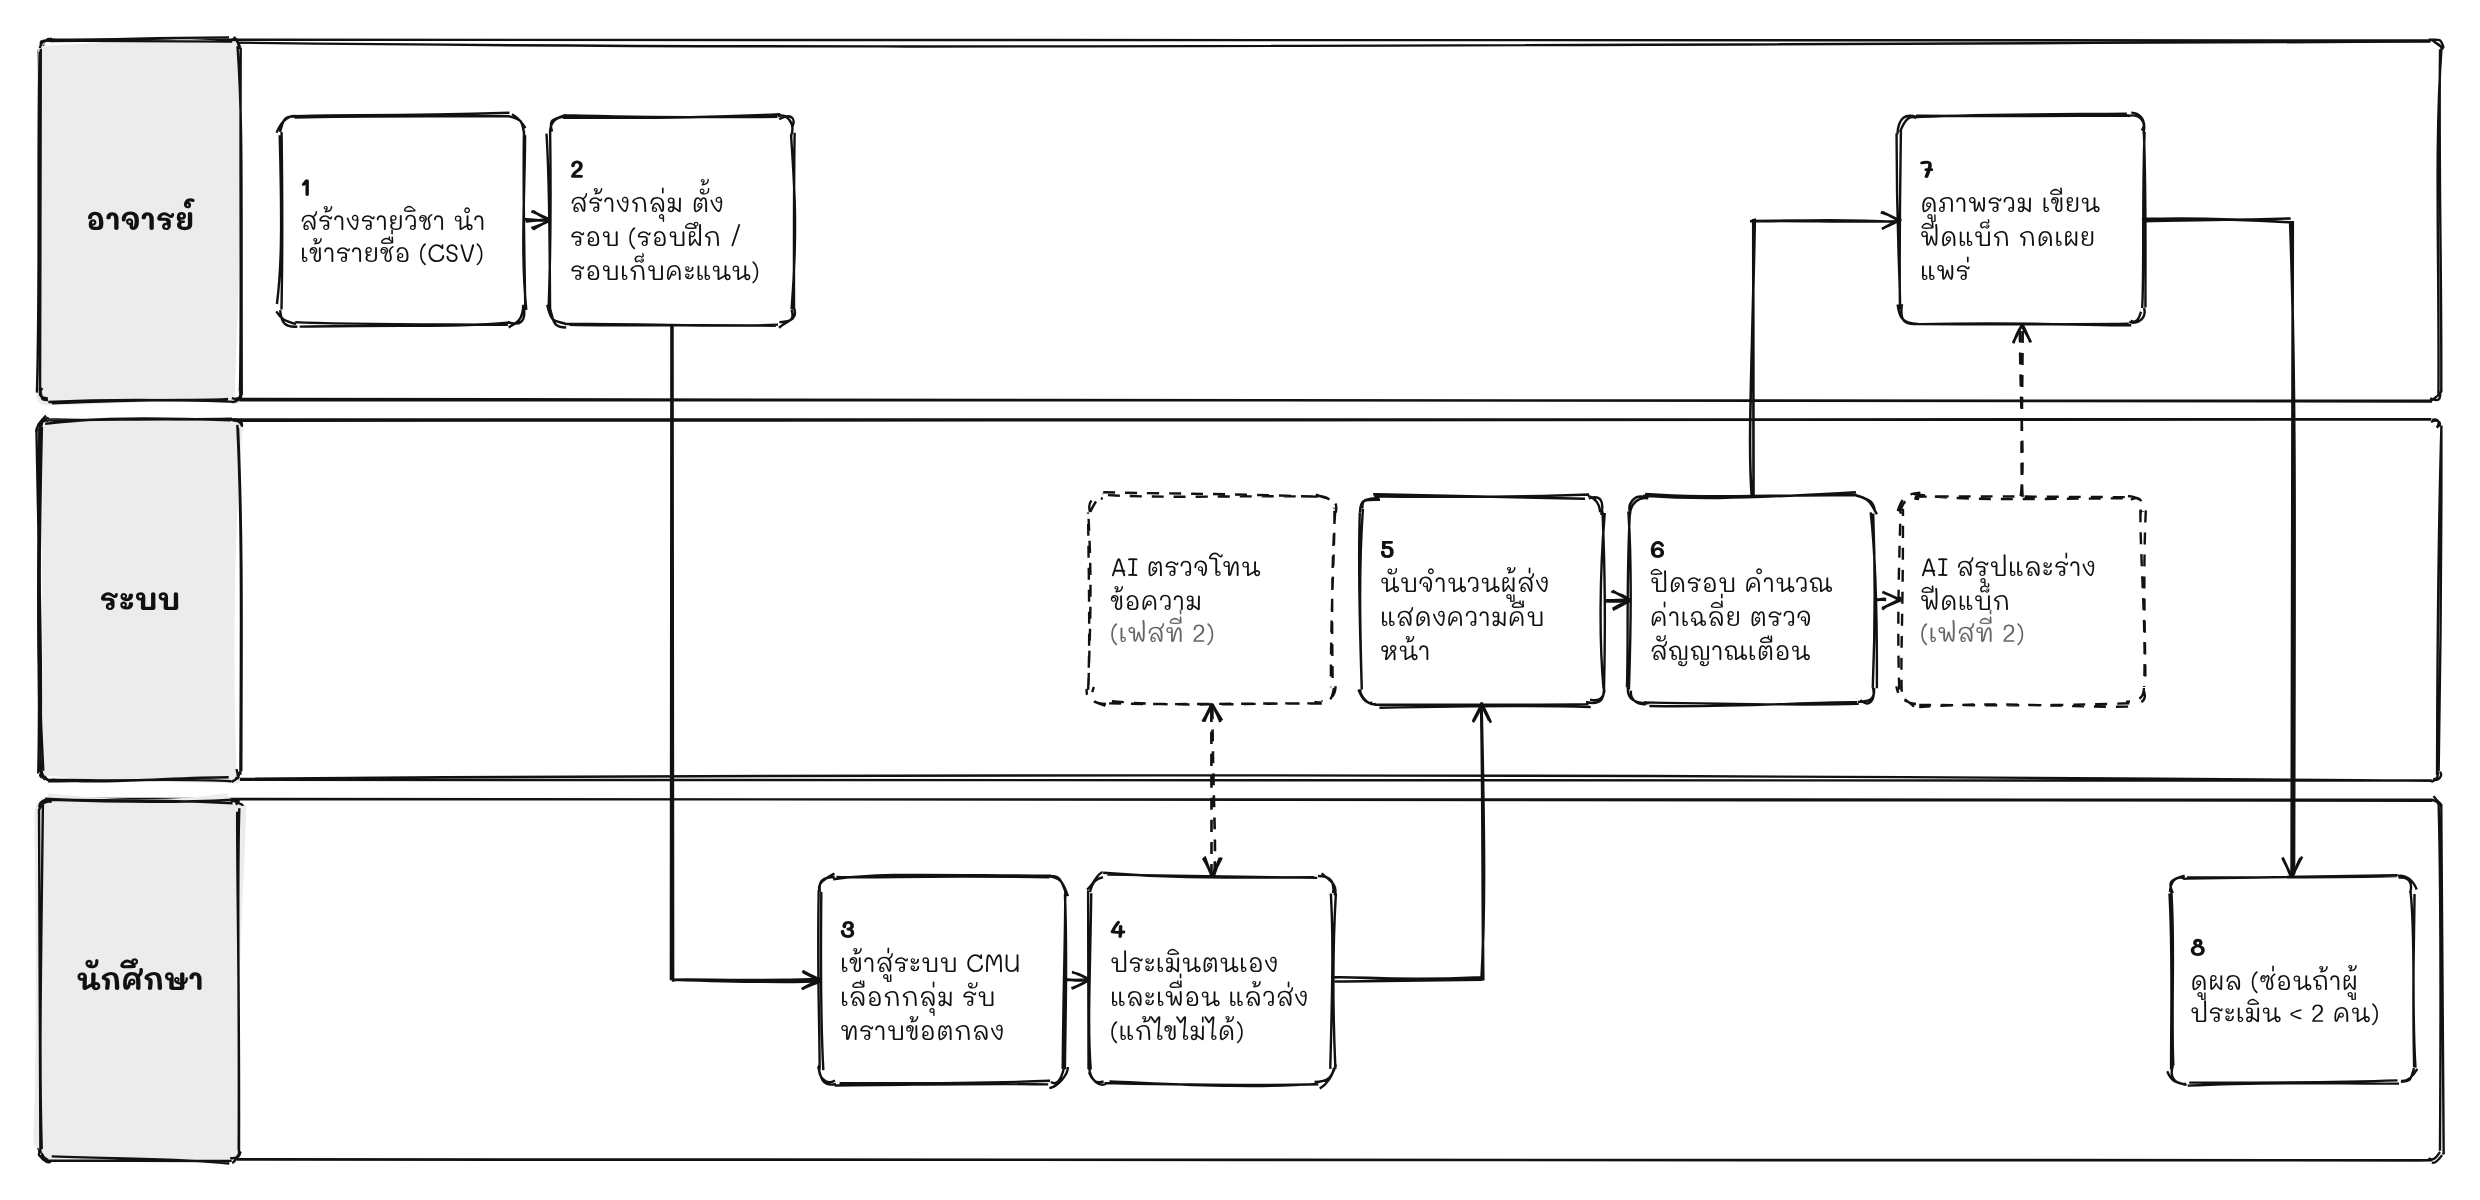
\includegraphics[width=\textwidth]{figures/ch3/fig3-1-swimlane.png}}{\fbox{\parbox{0.8\textwidth}{\centering\vspace{2cm}[วางไฟล์ figures/ch3/fig3-1-swimlane.png]\vspace{2cm}}}}
\caption{ขั้นตอนการทำงานของหนึ่งรอบประเมินแบบ swimlane}\label{fig:ch3-1}
\end{figure}

\subsection{การปกปิดตัวตนและสิทธิ์การมองเห็นข้อมูล}\label{sec:3.5.3}

ระบบไม่เปิดเผยตัวตนของผู้ประเมินต่อเพื่อน เพื่อให้นักศึกษากล้าให้ข้อเสนอแนะอย่างจริงใจ และให้นักศึกษาเห็นเฉพาะข้อมูลของตนเอง เพื่อลดการเปรียบเทียบและแข่งขันกันระหว่างเพื่อน สิทธิ์การมองเห็นข้อมูลแสดงในตารางที่~\ref{tab:ch3-8}

\begin{xltabular}{\textwidth}{|P{0.2\textwidth}|Y|P{0.12\textwidth}|Y|}
\caption{สิทธิ์การมองเห็นข้อมูลของผู้ใช้แต่ละบทบาท}\label{tab:ch3-8}\\
\hline \textbf{ข้อมูล} & \textbf{นักศึกษาเจ้าของข้อมูล} & \textbf{นักศึกษาคนอื่น} & \textbf{อาจารย์} \\ \hline
\endfirsthead
\multicolumn{4}{r}{\small (ต่อ)}\\ \hline \textbf{ข้อมูล} & \textbf{นักศึกษาเจ้าของข้อมูล} & \textbf{นักศึกษาคนอื่น} & \textbf{อาจารย์} \\ \hline
\endhead
คะแนนเฉลี่ยรายด้านที่เพื่อนประเมิน & เห็น เมื่อมีผู้ประเมินอย่างน้อย 2 คนและอาจารย์เผยแพร่แล้ว & ไม่เห็น & เห็น \\ \hline
คะแนนรายคนและชื่อผู้ประเมิน & ไม่เห็น & ไม่เห็น & เห็น เพื่อใช้ติดตามและกลั่นกรอง \\ \hline
ความเห็นปลายเปิด & เห็นหลังอาจารย์เผยแพร่ ในรูปแบบที่อาจารย์เลือก & ไม่เห็น & เห็นทั้งหมด \\ \hline
คะแนนที่ประเมินตนเอง & เห็น & ไม่เห็น & เห็น \\ \hline
สัญญาณเตือนและสถานะการส่ง & ไม่เห็น & ไม่เห็น & เห็น \\ \hline
\end{xltabular}

เงื่อนไขผู้ประเมินขั้นต่ำ 2 คนป้องกันไม่ให้นักศึกษาเดาได้ว่าใครเป็นผู้ประเมินในกรณีที่กลุ่มมีสมาชิกน้อย การบังคับสิทธิ์ทั้งหมดทำที่ฝั่ง API ไม่ใช่เพียงการซ่อนบนหน้าจอ ข้อมูลที่ผู้ใช้ไม่มีสิทธิ์จึงไม่ถูกส่งออกจากเซิร์ฟเวอร์เลย

\subsection{สัญญาณเตือน การเผยแพร่ผล และการสื่อสาร}\label{sec:3.5.4}

ในระยะที่ 1 ระบบสร้างสัญญาณเตือนจากรูปแบบคะแนนตามเงื่อนไขที่กำหนดไว้ (rule-based) เช่น คะแนนเฉลี่ยที่เพื่อนให้ต่ำในด้านใดด้านหนึ่ง คะแนนที่ประเมินตนเองต่างจากที่เพื่อนประเมินมาก หรือยังไม่ส่งแบบประเมิน เพื่อชี้ให้อาจารย์รู้ว่าควรดูแลทีมใดก่อน ฐานข้อมูลเก็บแหล่งที่มาของสัญญาณไว้ด้วย จึงรองรับสัญญาณจากปัญญาประดิษฐ์ (AI) ในระยะที่ 2 ได้โดยไม่ต้องเปลี่ยนโครงสร้าง

ผลการประเมินจะไม่ถึงนักศึกษาโดยอัตโนมัติ อาจารย์เป็นผู้ตรวจทานและกดเผยแพร่ทุกครั้ง โดยเลือกได้ว่าจะแสดงความเห็นของเพื่อนตามจริง หรือแสดงเป็นข้อสรุปที่อาจารย์เขียน การสื่อสารเป็นแบบทางเดียว นักศึกษาตอบกลับความเห็นของเพื่อนในระบบไม่ได้ เพราะการโต้ตอบอาจทำให้สืบทราบตัวตนผู้ประเมินได้ หากนักศึกษามีข้อสงสัยให้สื่อสารผ่านอาจารย์ นอกจากนี้ระบบออกแบบให้ใช้ร่วมกับกิจกรรมในชั้นเรียน เช่น อาจารย์อาจจัดเวลาประมาณ 1 ชั่วโมงให้นักศึกษาพูดคุยเรื่องข้อเสนอแนะกันแบบพบหน้า เพื่อไม่ให้การให้ข้อเสนอแนะผ่านระบบออนไลน์เพียงอย่างเดียวดูห่างเหิน

\section{การออกแบบส่วน AI (ระยะที่ 2)}\label{sec:3.6}

\subsection{ที่มาของการใช้ปัญญาประดิษฐ์}\label{sec:3.6.1}

การเรียนรู้ในปัจจุบันต้องปรับตัวกับการที่ทั้งผู้เรียนและผู้สอนใช้เครื่องมือปัญญาประดิษฐ์ (AI) มากขึ้น ระบบจึงนำปัญญาประดิษฐ์ มาใช้เฉพาะงานที่ปัญญาประดิษฐ์ (AI) ทำได้ดีและลดภาระคนได้จริง คือการอ่านและสรุปข้อความจำนวนมาก และการช่วยเกลาภาษา โดยไม่ให้ปัญญาประดิษฐ์ (AI) ตัดสินใจแทนคน ส่วนปัญญาประดิษฐ์ (AI) จัดอยู่ในการพัฒนาระยะที่ 2 โดยระบบใช้โมเดลภาษา Qwen ผ่าน API และแบ่งเป็น 2 ส่วน ดังรูปที่~\ref{fig:ch3-2}

\begin{figure}[htbp]
\centering
\IfFileExists{figures/ch3/fig3-2-ai.png}{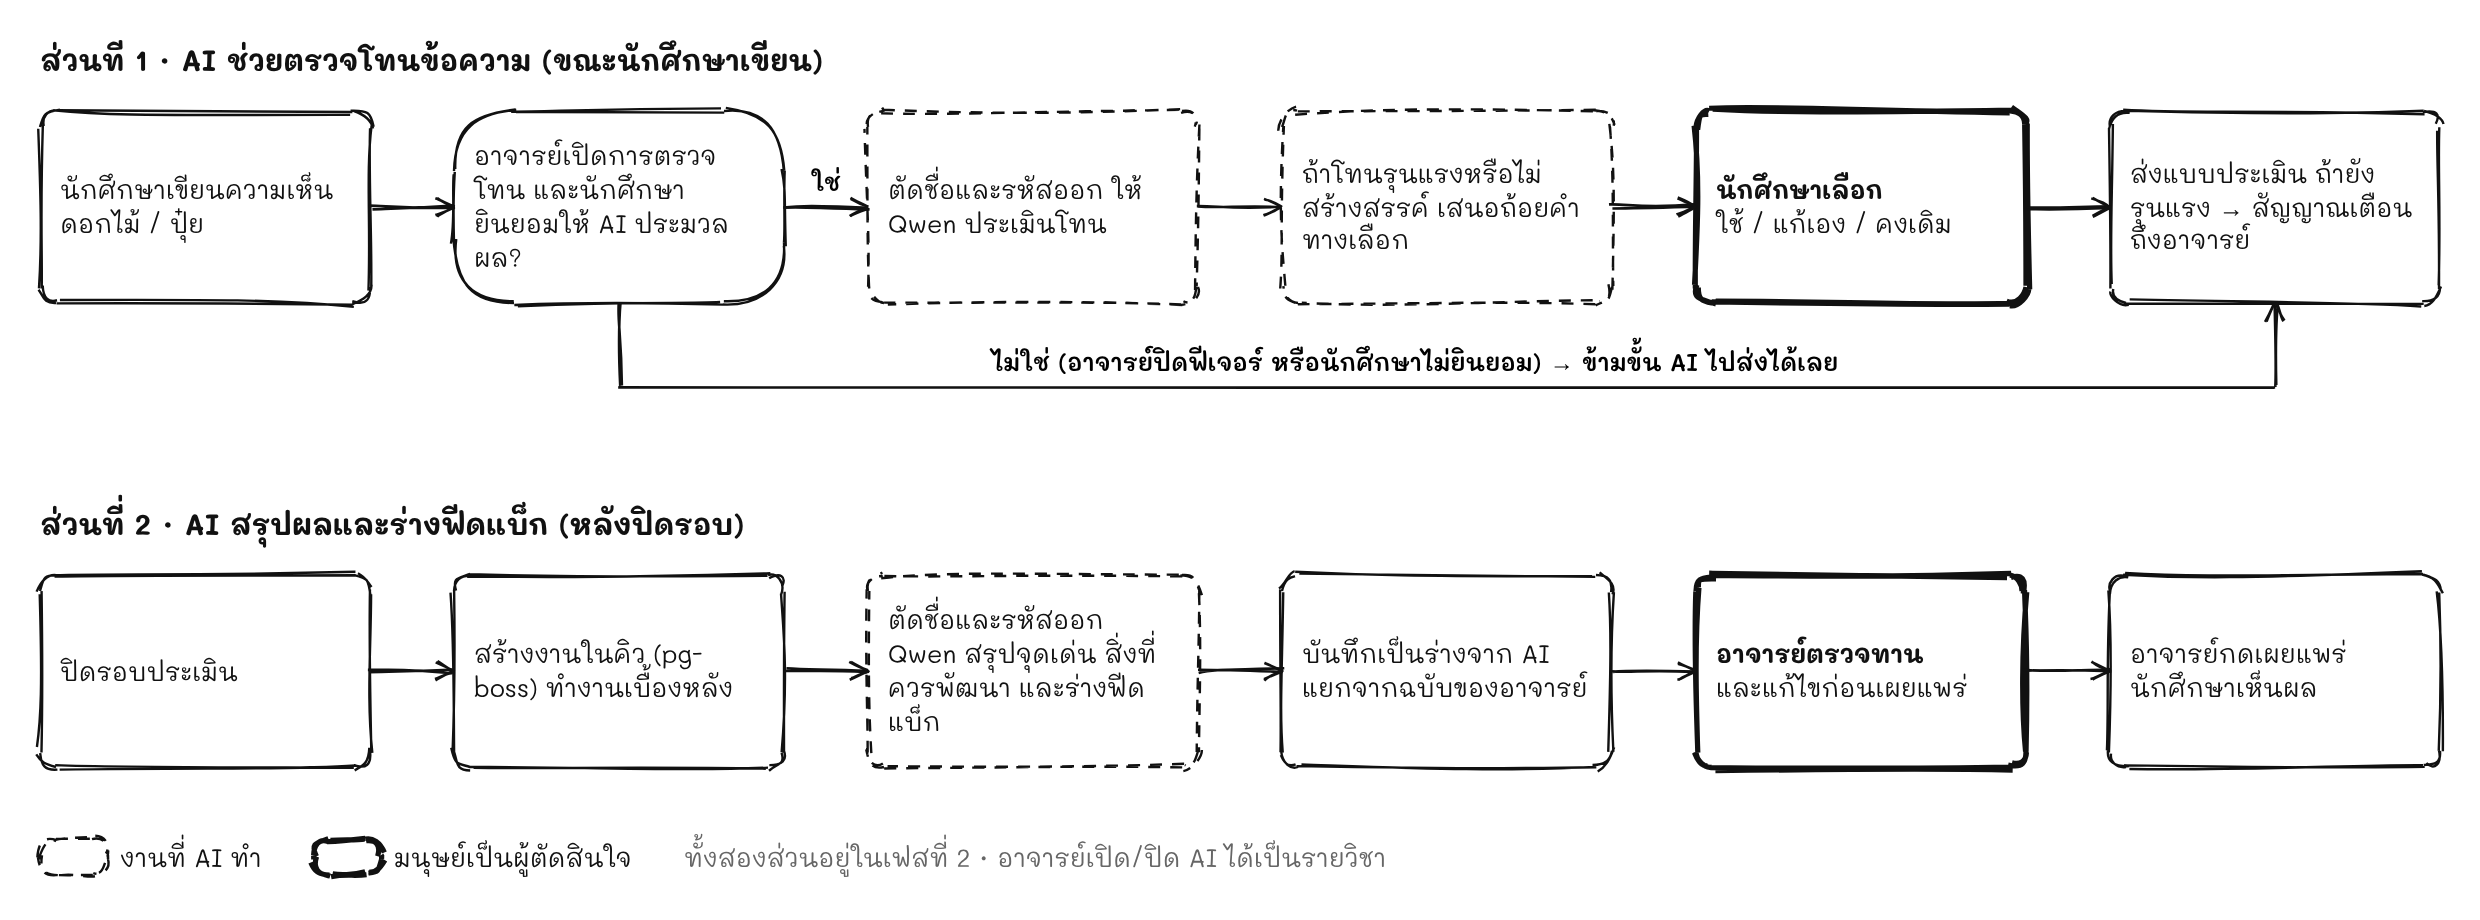
\includegraphics[width=\textwidth]{figures/ch3/fig3-2-ai.png}}{\fbox{\parbox{0.8\textwidth}{\centering\vspace{2cm}[วางไฟล์ figures/ch3/fig3-2-ai.png]\vspace{2cm}}}}
\caption{การทำงานของส่วน AI ทั้ง 2 ส่วน}\label{fig:ch3-2}
\end{figure}

\subsection{ปัญญาประดิษฐ์ช่วยตรวจโทนข้อความ}\label{sec:3.6.2}

อาจารย์เลือกเปิดหรือปิดฟีเจอร์นี้ได้เป็นรายวิชา เมื่อเปิดใช้งาน ขณะนักศึกษาเขียนความเห็นปลายเปิด ระบบส่งข้อความให้โมเดลประเมินโทน หากข้อความมีลักษณะรุนแรง ตำหนิตัวบุคคล หรือไม่สร้างสรรค์ ระบบจะแสดงคำเตือนพร้อมเสนอถ้อยคำทางเลือกที่สื่อประเด็นเดิมอย่างสร้างสรรค์ นักศึกษาเป็นผู้ตัดสินใจเองว่าจะใช้ถ้อยคำที่เสนอ แก้ไขเอง หรือคงข้อความเดิม ระบบไม่เปลี่ยนข้อความให้โดยอัตโนมัติ หากข้อความที่ส่งแล้วยังมีโทนรุนแรง ระบบจะบันทึกเป็นสัญญาณเตือนให้อาจารย์เห็น หากอาจารย์ปิดฟีเจอร์นี้ นักศึกษาจะเขียนและส่งความเห็นได้ตามปกติโดยไม่ผ่านการตรวจโทน

\subsection{ปัญญาประดิษฐ์สรุปผลและร่างข้อเสนอแนะ}\label{sec:3.6.3}

เมื่อปิดรอบประเมิน ระบบรวบรวมความเห็นที่นักศึกษาแต่ละคนได้รับ แล้วส่งให้โมเดลสรุปเป็นจุดเด่นและสิ่งที่ควรพัฒนา พร้อมร่างข้อเสนอแนะถึงนักศึกษาคนนั้น ร่างจากปัญญาประดิษฐ์ (AI) ถูกเก็บแยกจากฉบับที่อาจารย์แก้ไข และอาจารย์ต้องตรวจทานก่อนเผยแพร่ทุกครั้ง การประมวลผลทำผ่านคิวงานเบื้องหลัง ผู้ใช้จึงไม่ต้องรอระหว่างที่โมเดลทำงาน

\subsection{หลักการกำกับการใช้ปัญญาประดิษฐ์ (AI)}\label{sec:3.6.4}

\begin{itemize}
  \item มนุษย์ตัดสินใจขั้นสุดท้ายเสมอ (human-in-the-loop): AI ทำหน้าที่เสนอ ส่วนนักศึกษาและอาจารย์เป็นผู้เลือก
  \item เปิดหรือปิดได้: อาจารย์เปิดหรือปิดฟีเจอร์ปัญญาประดิษฐ์ (AI) ได้เป็นรายวิชา และข้อความของนักศึกษาจะถูกส่งให้ปัญญาประดิษฐ์ (AI) เฉพาะเมื่อนักศึกษายินยอมในส่วนทางเลือก (หัวข้อ~\ref{sec:3.9.2})
  \item ลดข้อมูลที่ส่งออก: ส่งเฉพาะข้อความที่ต้องประมวลผล โดยไม่ส่งชื่อหรือรหัสนักศึกษาไปยังผู้ให้บริการโมเดล
  \item ยอมรับข้อจำกัด: โมเดลอาจตีความภาษาไทยผิด โดยเฉพาะถ้อยคำประชดประชันซึ่งจัดเป็นงานในระยะที่ 3 นี่คือเหตุผลที่ระบบไม่ให้ปัญญาประดิษฐ์ (AI) ตัดสินใจเอง
\end{itemize}

\section{สถาปัตยกรรมระบบและฐานข้อมูล}\label{sec:3.7}

\subsection{ภาพรวมสถาปัตยกรรม}\label{sec:3.7.1}

ระบบเป็นเว็บแอปพลิเคชันที่แยกส่วนหน้า (frontend) และส่วนหลัง (backend) ออกจากกัน และสื่อสารกันผ่าน REST API ด้วยข้อมูลรูปแบบ JSON องค์ประกอบหลักแสดงในรูปที่~\ref{fig:ch3-3} ดังนี้

\begin{itemize}
  \item ส่วนหน้า: React 19, Vite และ TypeScript จัดหน้าตาด้วย Tailwind CSS จัดการข้อมูลจากเซิร์ฟเวอร์ด้วย TanStack Query และจัดการสถานะภายในหน้าเว็บด้วย Zustand
  \item เว็บเซิร์ฟเวอร์: nginx ให้บริการไฟล์ของส่วนหน้า ทำหน้าที่ reverse proxy ไปยัง API และจัดการ HTTPS
  \item ส่วนหลัง: Node.js และ Express 5 เข้าถึงฐานข้อมูลผ่าน Drizzle ORM และกำหนดสัญญาการเชื่อมต่อ API ด้วย OpenAPI
  \item ฐานข้อมูล: PostgreSQL เก็บข้อมูลของระบบ เซสชันผู้ใช้ และคิวงานเบื้องหลัง (pg-boss)
  \item Worker และบริการ AI (เฟสที่ 2): worker ดึงงานจากคิวไปเรียกโมเดล Qwen ผ่าน API แล้วบันทึกผลกลับลงฐานข้อมูล
\end{itemize}

คณะผู้จัดทำเลือกใช้ PostgreSQL เป็นทั้งที่เก็บเซสชันและคิวงาน แทนการเพิ่ม Redis และ BullMQ ซึ่งเป็นอีกทางเลือกหนึ่ง เพื่อลดจำนวนบริการที่ต้องดูแลและใช้ทรัพยากรน้อยลง ทางเลือกนี้เหมาะกับข้อจำกัดของเซิร์ฟเวอร์ขนาด 2 vCPU หน่วยความจำ 4 GB ตามงบประมาณของโครงงาน และปริมาณงานของระบบในระดับรายวิชาซึ่งไม่ได้ต้องการความเร็วที่สูงมาก

\begin{figure}[htbp]
\centering
\IfFileExists{figures/ch3/fig3-3-architecture.png}{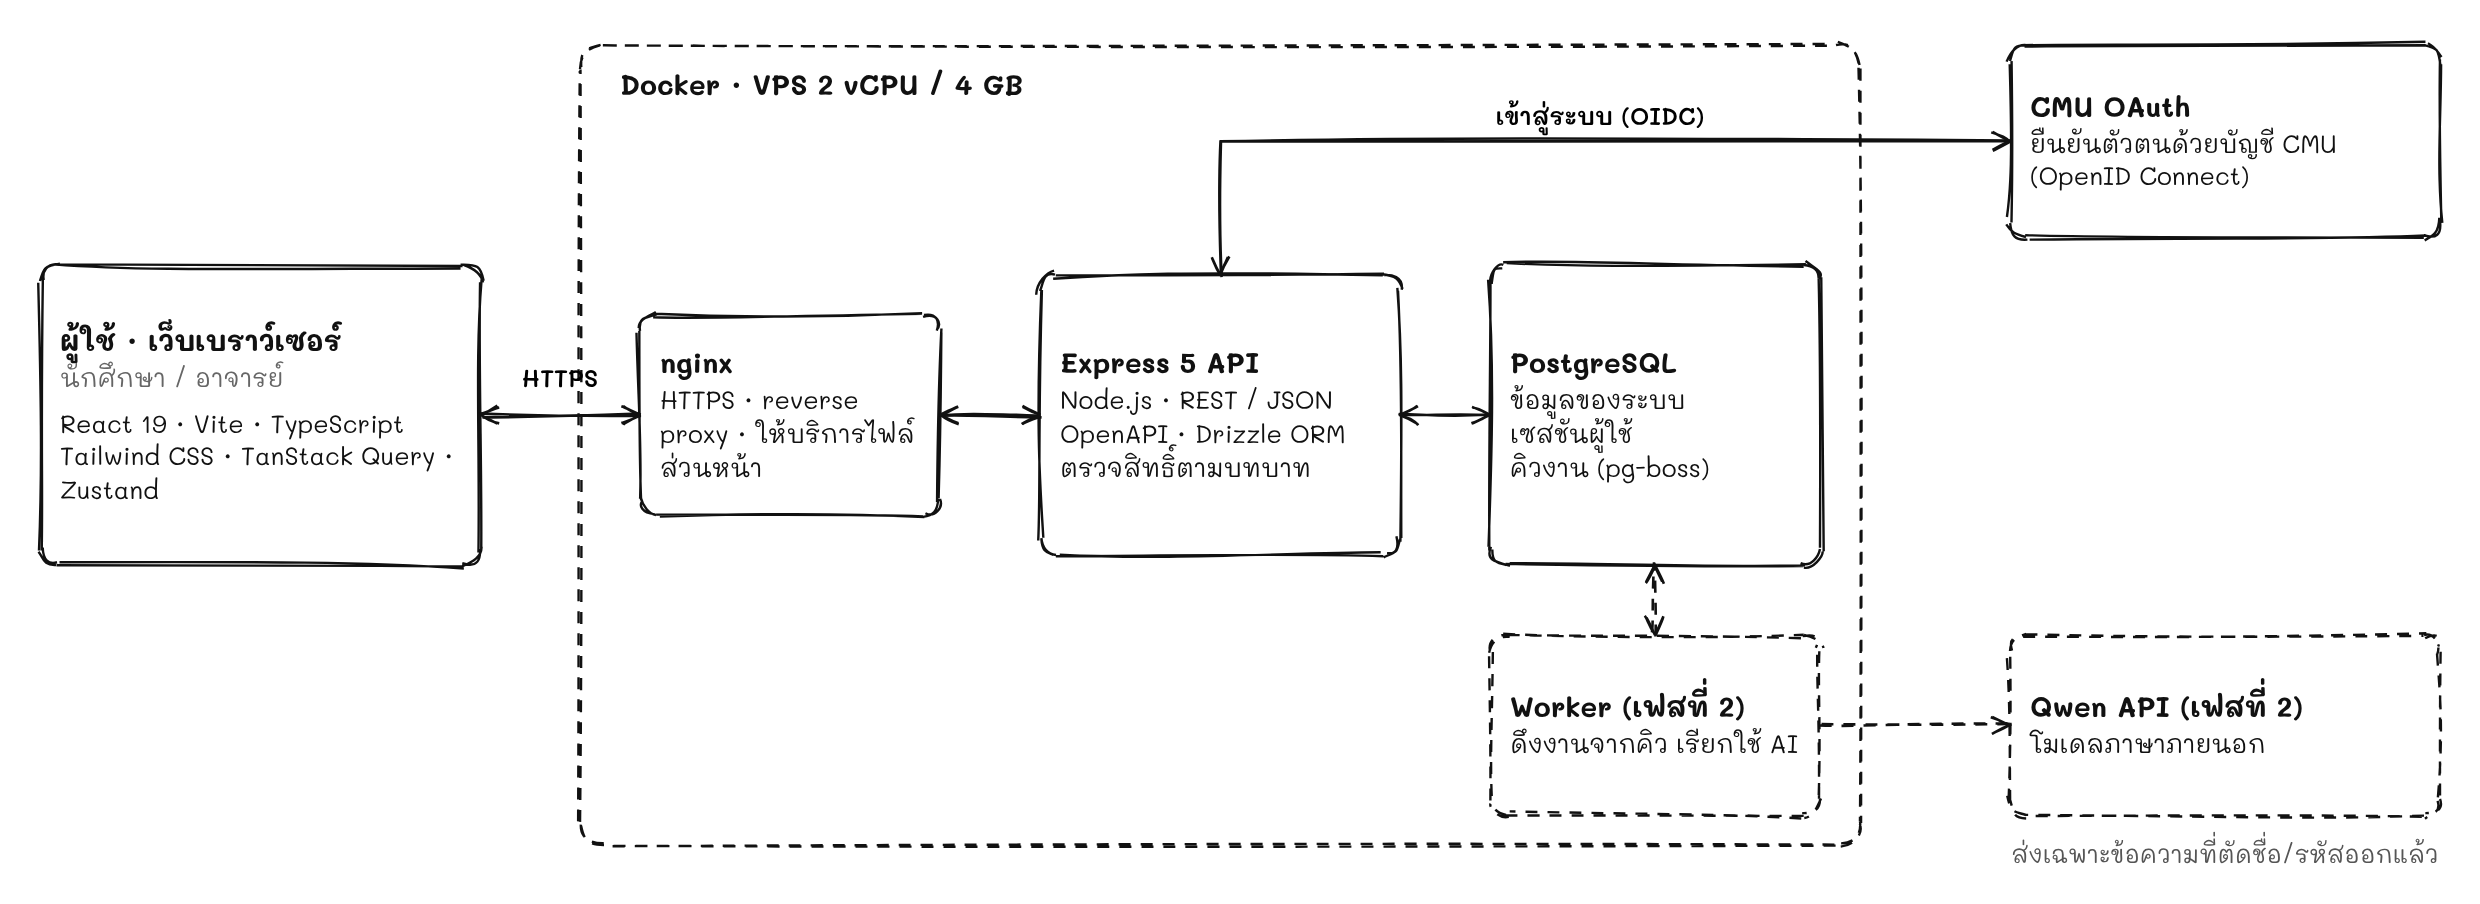
\includegraphics[width=\textwidth]{figures/ch3/fig3-3-architecture.png}}{\fbox{\parbox{0.8\textwidth}{\centering\vspace{2cm}[วางไฟล์ figures/ch3/fig3-3-architecture.png]\vspace{2cm}}}}
\caption{สถาปัตยกรรมของระบบ}\label{fig:ch3-3}
\end{figure}

\subsection{การยืนยันตัวตน}\label{sec:3.7.2}

ผู้ใช้เข้าสู่ระบบด้วยบัญชี CMU ผ่าน CMU OAuth ตามมาตรฐาน OpenID Connect~\cite{sakimura2014oidc} ระบบจึงไม่ต้องเก็บรหัสผ่านของผู้ใช้เอง หลังยืนยันตัวตน เซิร์ฟเวอร์สร้างเซสชันที่เก็บในฐานข้อมูล และส่งคุกกี้เซสชันแบบ HttpOnly และ Secure ให้เบราว์เซอร์ บทบาทของผู้ใช้ในแต่ละรายวิชา (นักศึกษาหรืออาจารย์) ถูกตรวจสอบทุกครั้งที่เรียก API

\subsection{การออกแบบฐานข้อมูล}\label{sec:3.7.3}

ฐานข้อมูลเป็นแบบเชิงสัมพันธ์ ประกอบด้วยตารางที่ระยะที่ 1 ใช้ และตารางที่เตรียมไว้สำหรับระยะถัดไป ได้แก่ ตารางสัญญาณเตือน (flags) และตารางสรุปผล (ai\_feedback\_summaries) สำหรับปัญญาประดิษฐ์ (AI) และตารางบันทึกการซิงก์ข้อมูล (external\_sync\_logs) สำหรับการเชื่อมต่อระบบภายนอก ความสัมพันธ์ของข้อมูลแสดงในรูปที่~\ref{fig:ch3-4} โดยมีการตัดสินใจออกแบบที่สำคัญดังนี้

\begin{itemize}
  \item ตารางคะแนน (ratings) ให้ช่องผู้ถูกประเมินเป็นค่าว่างได้ เพื่อรองรับคำถามระดับทีมที่ไม่ได้ประเมินบุคคลใดบุคคลหนึ่ง
  \item ตารางสรุปผล (ai\_feedback\_summaries) เก็บทั้งร่างจากปัญญาประดิษฐ์ (AI) และฉบับสุดท้ายที่อาจารย์แก้ไข เพื่อแยกให้เห็นว่าส่วนใดมาจากปัญญาประดิษฐ์ (AI) และส่วนใดผ่านการตรวจทานแล้ว
  \item ตารางความยินยอม (consents) เก็บเวอร์ชันของนโยบายที่ผู้ใช้ยินยอม เพื่อขอความยินยอมใหม่ได้เมื่อนโยบายเปลี่ยน
  \item ตารางสัญญาณเตือน (flags) มีช่องระบุแหล่งที่มาของสัญญาณ เพื่อรองรับทั้งสัญญาณจากเงื่อนไขคะแนนและจากปัญญาประดิษฐ์ (AI)
  \item ตารางรายวิชาและผู้ใช้มีช่องเก็บรหัสอ้างอิงจากระบบภายนอก เพื่อเตรียมเชื่อมต่อ Mango Canvas ในระยะที่ 3 โดยมีตารางบันทึกการซิงก์ข้อมูล (external\_sync\_logs) เก็บผลการนำเข้ารายชื่อและส่งออกคะแนนของแต่ละรายวิชา
  \item ตารางระดับเกณฑ์การให้คะแนน (rubric\_levels) เก็บคำอธิบายพฤติกรรมของแต่ละคะแนนในคำถามแบบให้คะแนน เพื่อให้ผู้ประเมินใช้เกณฑ์เดียวกัน
\end{itemize}

\begin{sidewaysfigure}
\centering
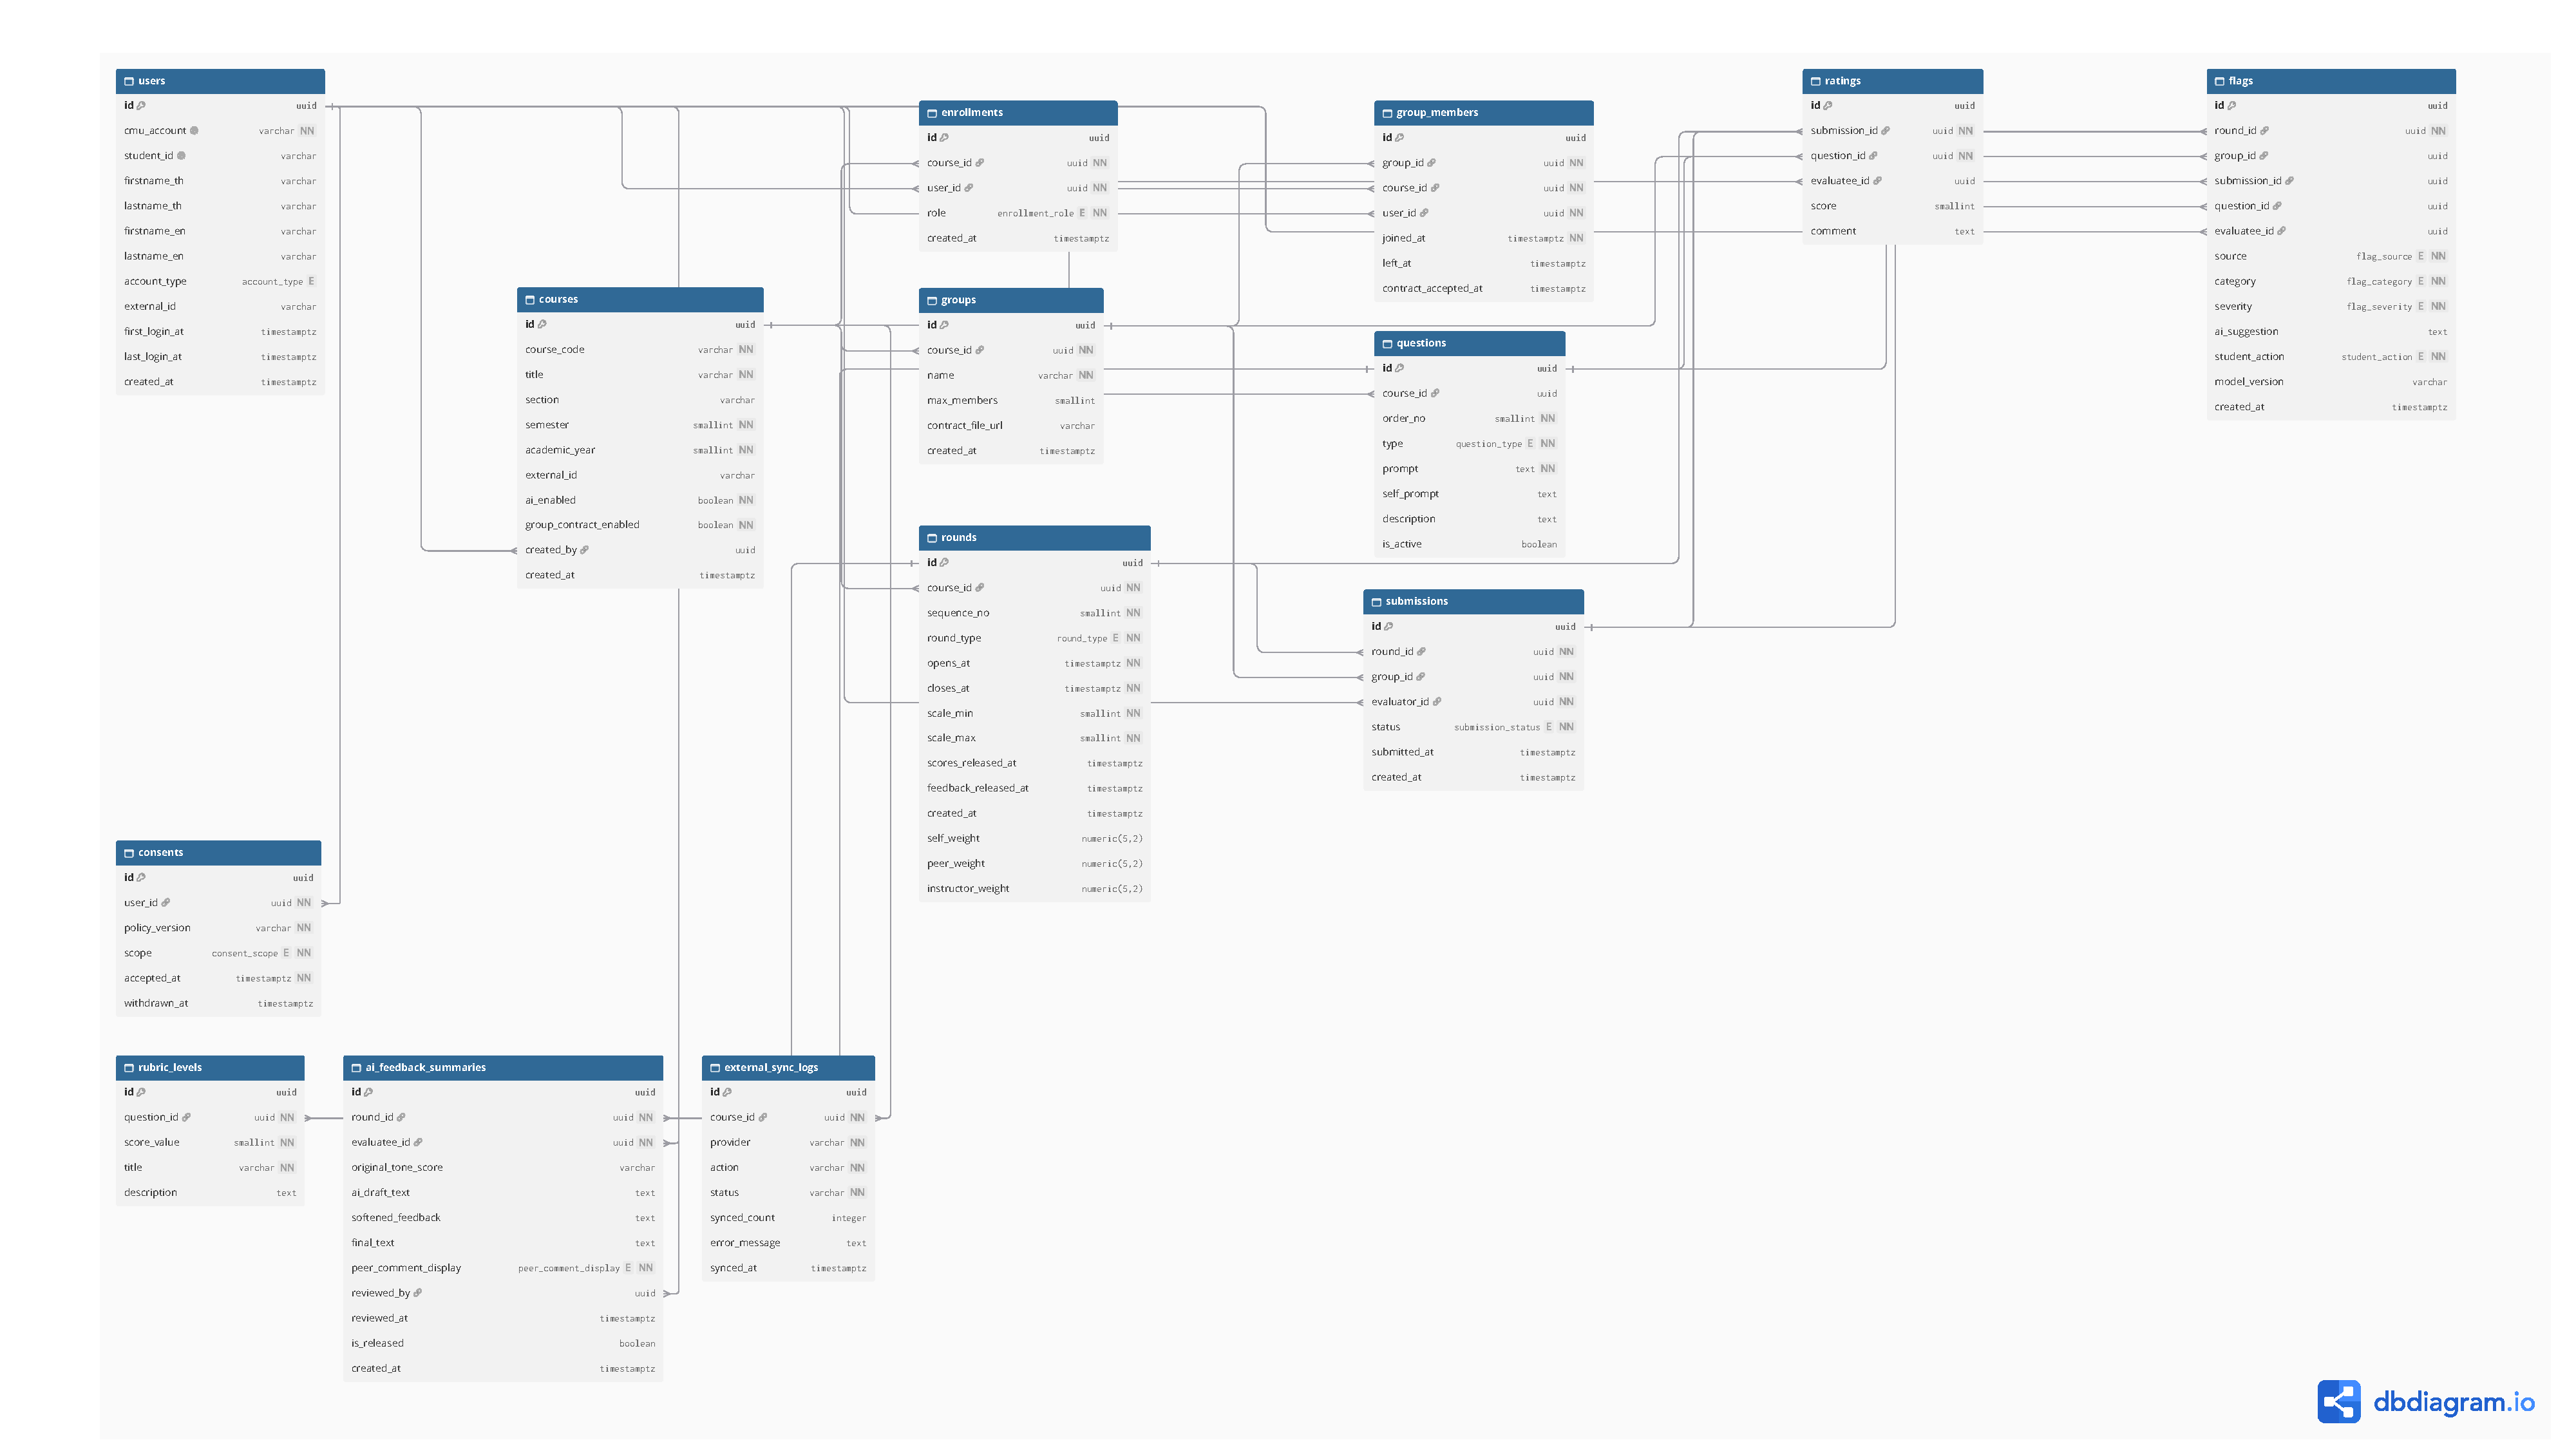
\includegraphics[width=\linewidth]{figures/ch3/fig3-4-er.pdf}
\caption{แผนภาพความสัมพันธ์ของข้อมูล (ER diagram)}\label{fig:ch3-4}
\end{sidewaysfigure}

\subsection{การติดตั้งและการทดสอบ}\label{sec:3.7.4}

ทุกบริการถูกบรรจุเป็น Docker container และติดตั้งบนเซิร์ฟเวอร์เสมือน (VPS) ขนาด 2 vCPU หน่วยความจำ 4 GB การทดสอบใช้ Vitest สำหรับ unit test และ integration test และใช้ Cypress สำหรับ end-to-end test ส่วนการสำรองข้อมูล การตรวจสอบสถานะระบบ และการส่งอีเมล ใช้บริการแบบไม่มีค่าใช้จ่าย

\section{การออกแบบส่วนต่อประสานผู้ใช้}\label{sec:3.8}

\subsection{หลักการออกแบบ}\label{sec:3.8.1}

\begin{itemize}
  \item นำทางตามงาน: แถบเมนูด้านข้างจัดตามงานที่ผู้ใช้ต้องทำ พร้อมตัวเลขแจ้งจำนวนงานค้าง
  \item แสดงสถานะด้วยป้ายสถานะ (status pill) เช่น เปิดรับ ปิดแล้ว และรอเผยแพร่
  \item แบบประเมินแสดงทีละคำถามต่อหน้าจอ เพื่อลดภาระการอ่านและใช้งานบนมือถือได้สะดวก
  \item ออกแบบตามแนวทาง WCAG 2.2~\cite{w3c2023wcag} เช่น ความต่างของสีตัวอักษรกับพื้นหลังที่เพียงพอ การใช้งานด้วยแป้นพิมพ์ และการติดป้ายกำกับช่องกรอกทุกช่อง
\end{itemize}

หน้าจอทั้งหมดออกแบบเป็นต้นแบบความละเอียดต่ำ (low-fidelity wireframe) แบบขาวดำก่อนพัฒนาจริง และใช้ต้นแบบนี้สื่อสารทั้งภายในทีมและกับอาจารย์ผู้ใช้ เพื่อรับความคิดเห็นก่อนลงมือพัฒนา

\subsection{หน้าจอฝั่งนักศึกษา}\label{sec:3.8.2}

ผู้ใช้เข้าสู่ระบบด้วยบัญชี CMU ผ่าน CMU OAuth โดยไม่ต้องสร้างรหัสผ่านใหม่ ดังรูปที่~\ref{fig:ch3-5}

\begin{figure}[htbp]
\centering
\IfFileExists{figures/ch3/fig3-5-login.png}{
\includegraphics[width=\textwidth]{figures/ch3/fig3-5-login.png}}{\fbox{\parbox{0.8\textwidth}{\centering\vspace{2cm}[วางไฟล์ figures/ch3/fig3-5-login.png]\vspace{2cm}}}}
\caption{หน้าเข้าสู่ระบบ}\label{fig:ch3-5}
\end{figure}

ครั้งแรกที่เข้าใช้งาน นักศึกษาต้องอ่านข้อตกลงการใช้ข้อมูลส่วนบุคคล ซึ่งแบ่งจอเป็น 2 ส่วน ด้านซ้ายย้ำว่าความเห็นถึงเพื่อนจะไม่ระบุชื่อ ด้านขวาแสดงว่าเก็บข้อมูลอะไร ใครเห็น เก็บนานเท่าใด และสิทธิ์ของเจ้าของข้อมูล พร้อมตัวเลือกส่วนจำเป็นและส่วนทางเลือก ดังรูปที่~\ref{fig:ch3-6}

\begin{figure}[htbp]
\centering
\IfFileExists{figures/ch3/fig3-6-consent.png}{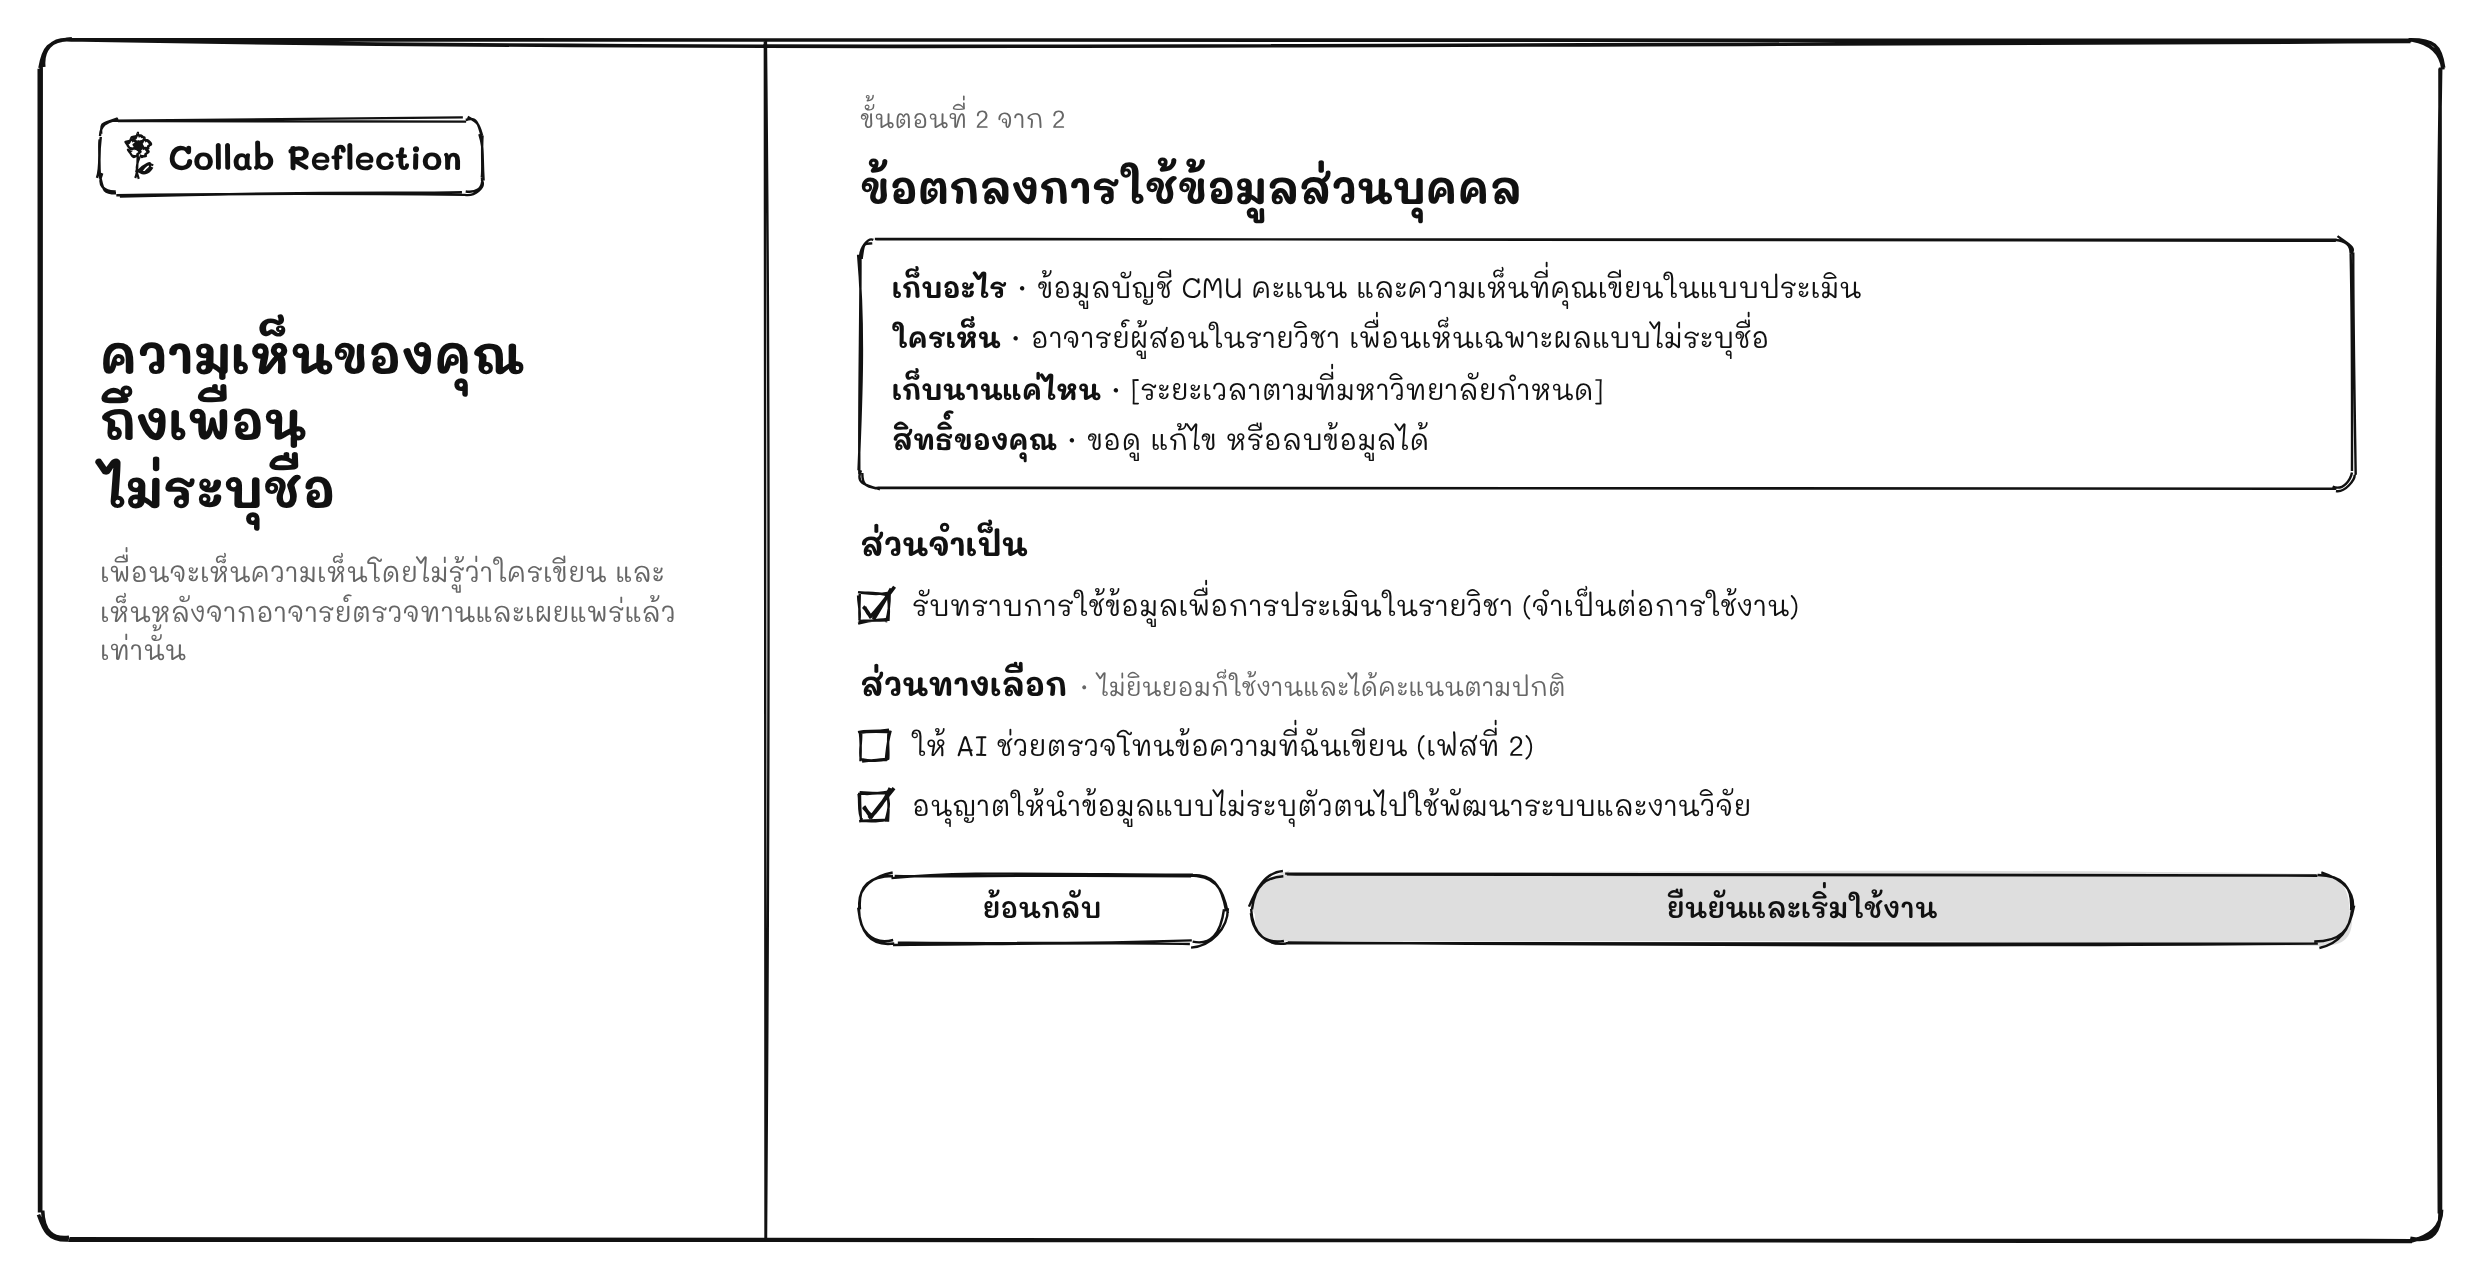
\includegraphics[width=\textwidth]{figures/ch3/fig3-6-consent.png}}{\fbox{\parbox{0.8\textwidth}{\centering\vspace{2cm}[วางไฟล์ figures/ch3/fig3-6-consent.png]\vspace{2cm}}}}
\caption{หน้าข้อตกลงการใช้ข้อมูลส่วนบุคคล}\label{fig:ch3-6}
\end{figure}

หน้ารายวิชาแสดงกลุ่มของนักศึกษา ข้อตกลงกลุ่ม และรายการรอบประเมิน โดยทุกรอบมีป้ายบอกว่าเป็นรอบฝึกหรือรอบเก็บคะแนน พร้อมสถานะของรอบ ดังรูปที่~\ref{fig:ch3-7}

\begin{figure}[htbp]
\centering
\IfFileExists{figures/ch3/fig3-7-student-course.png}{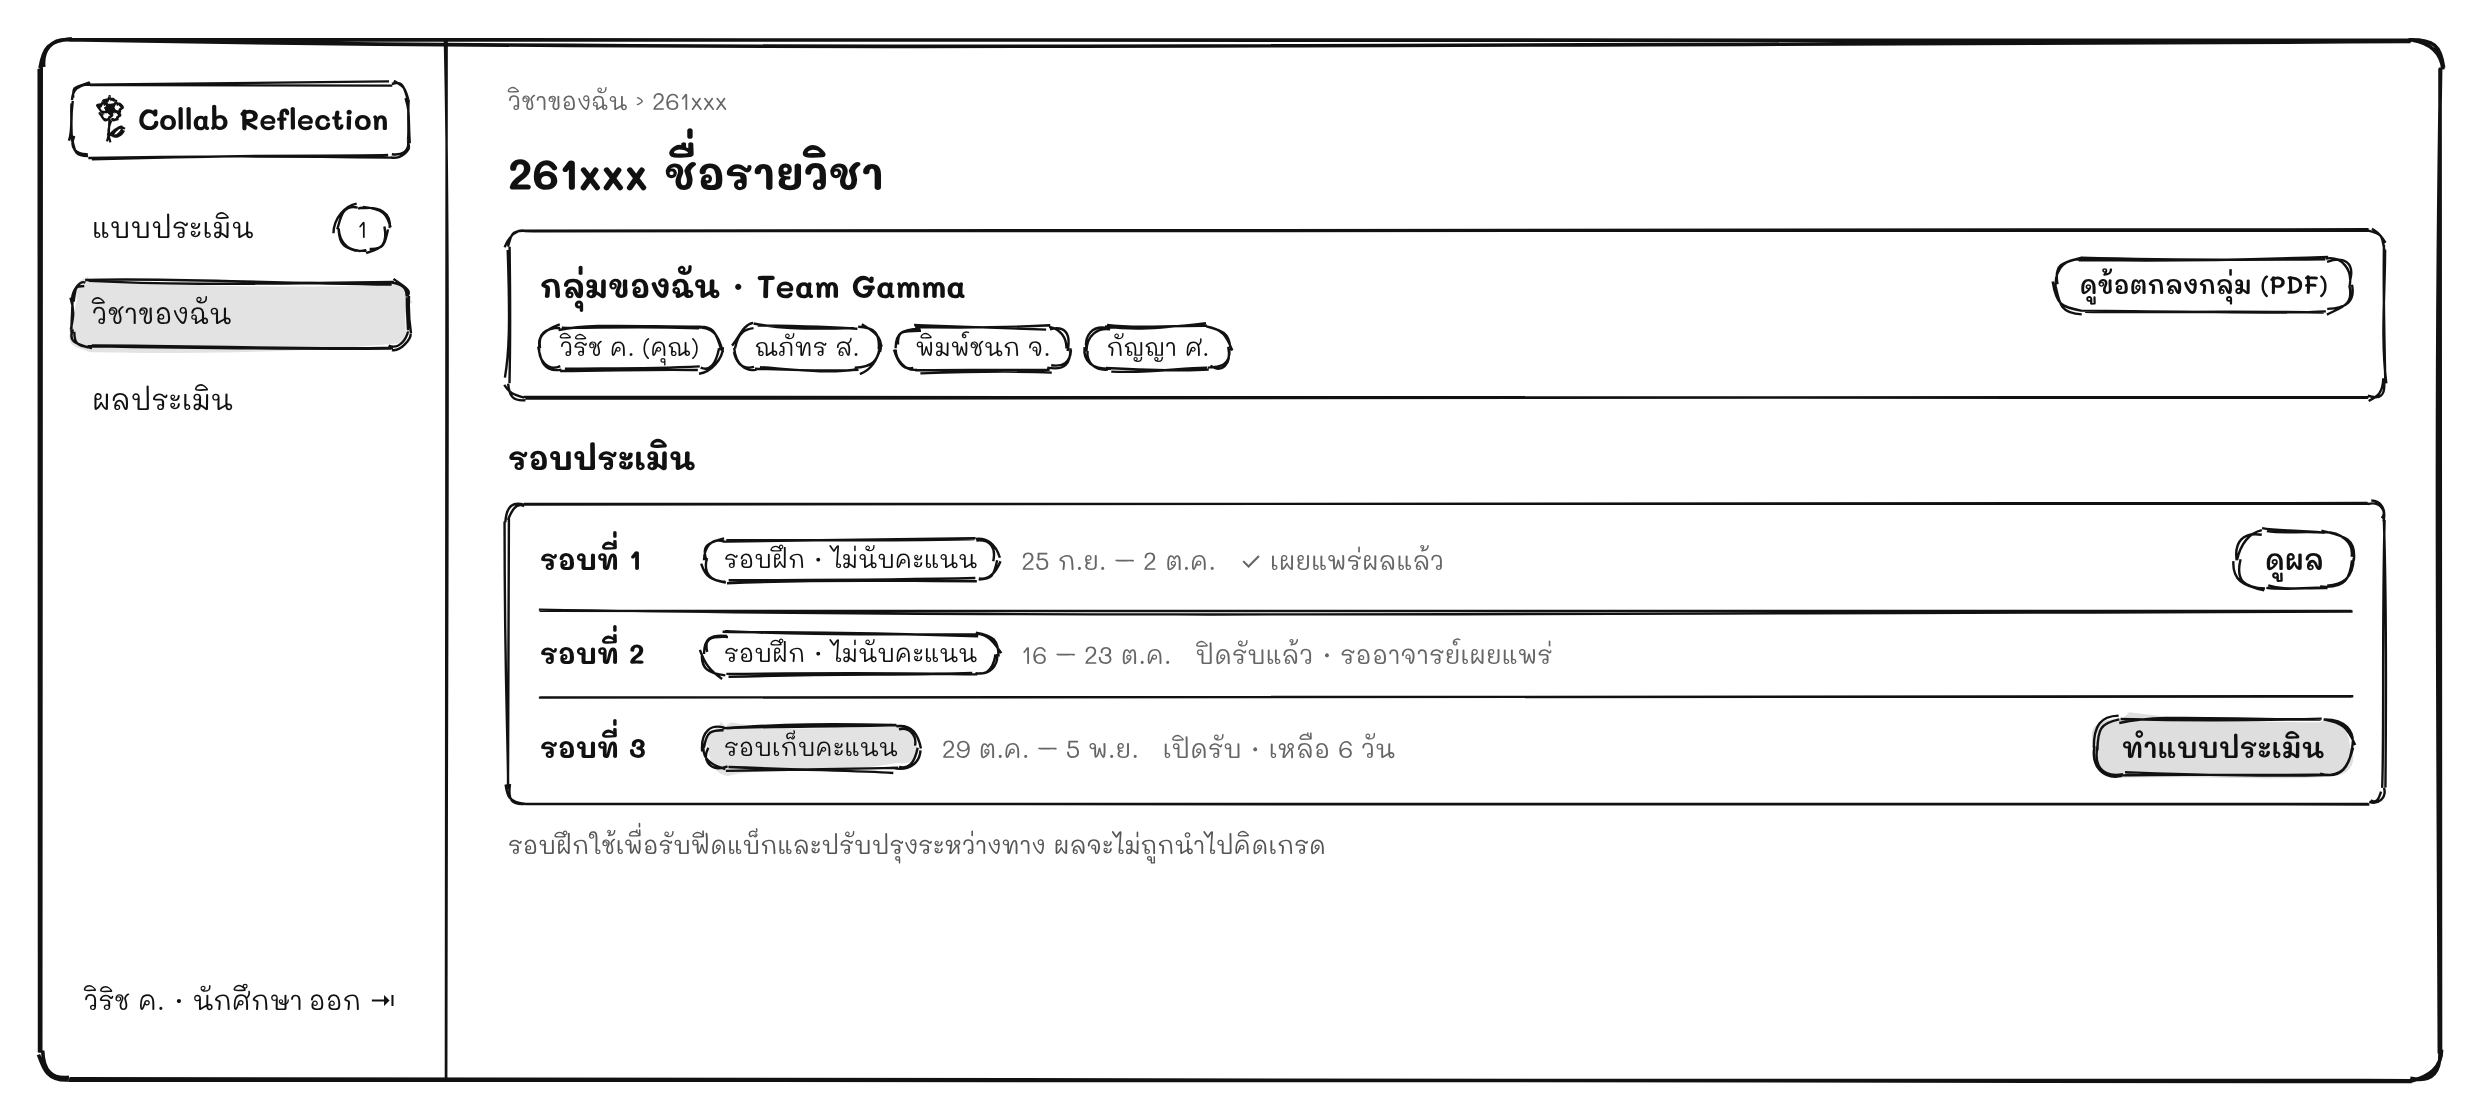
\includegraphics[width=\textwidth]{figures/ch3/fig3-7-student-course.png}}{\fbox{\parbox{0.8\textwidth}{\centering\vspace{2cm}[วางไฟล์ figures/ch3/fig3-7-student-course.png]\vspace{2cm}}}}
\caption{หน้ารายวิชาและรอบประเมินของนักศึกษา}\label{fig:ch3-7}
\end{figure}

แบบประเมินแสดงทีละด้านต่อหน้าจอ ด้านบนมีคำอธิบายพฤติกรรมของระดับ 1, 3 และ 5 ให้นักศึกษาให้คะแนนสมาชิกทุกคนรวมถึงตนเอง และด้านขวามีแถบแสดงขั้นตอนทั้ง 7 ขั้น ดังรูปที่~\ref{fig:ch3-8}

\begin{figure}[htbp]
\centering
\IfFileExists{figures/ch3/fig3-8-student-rating.png}{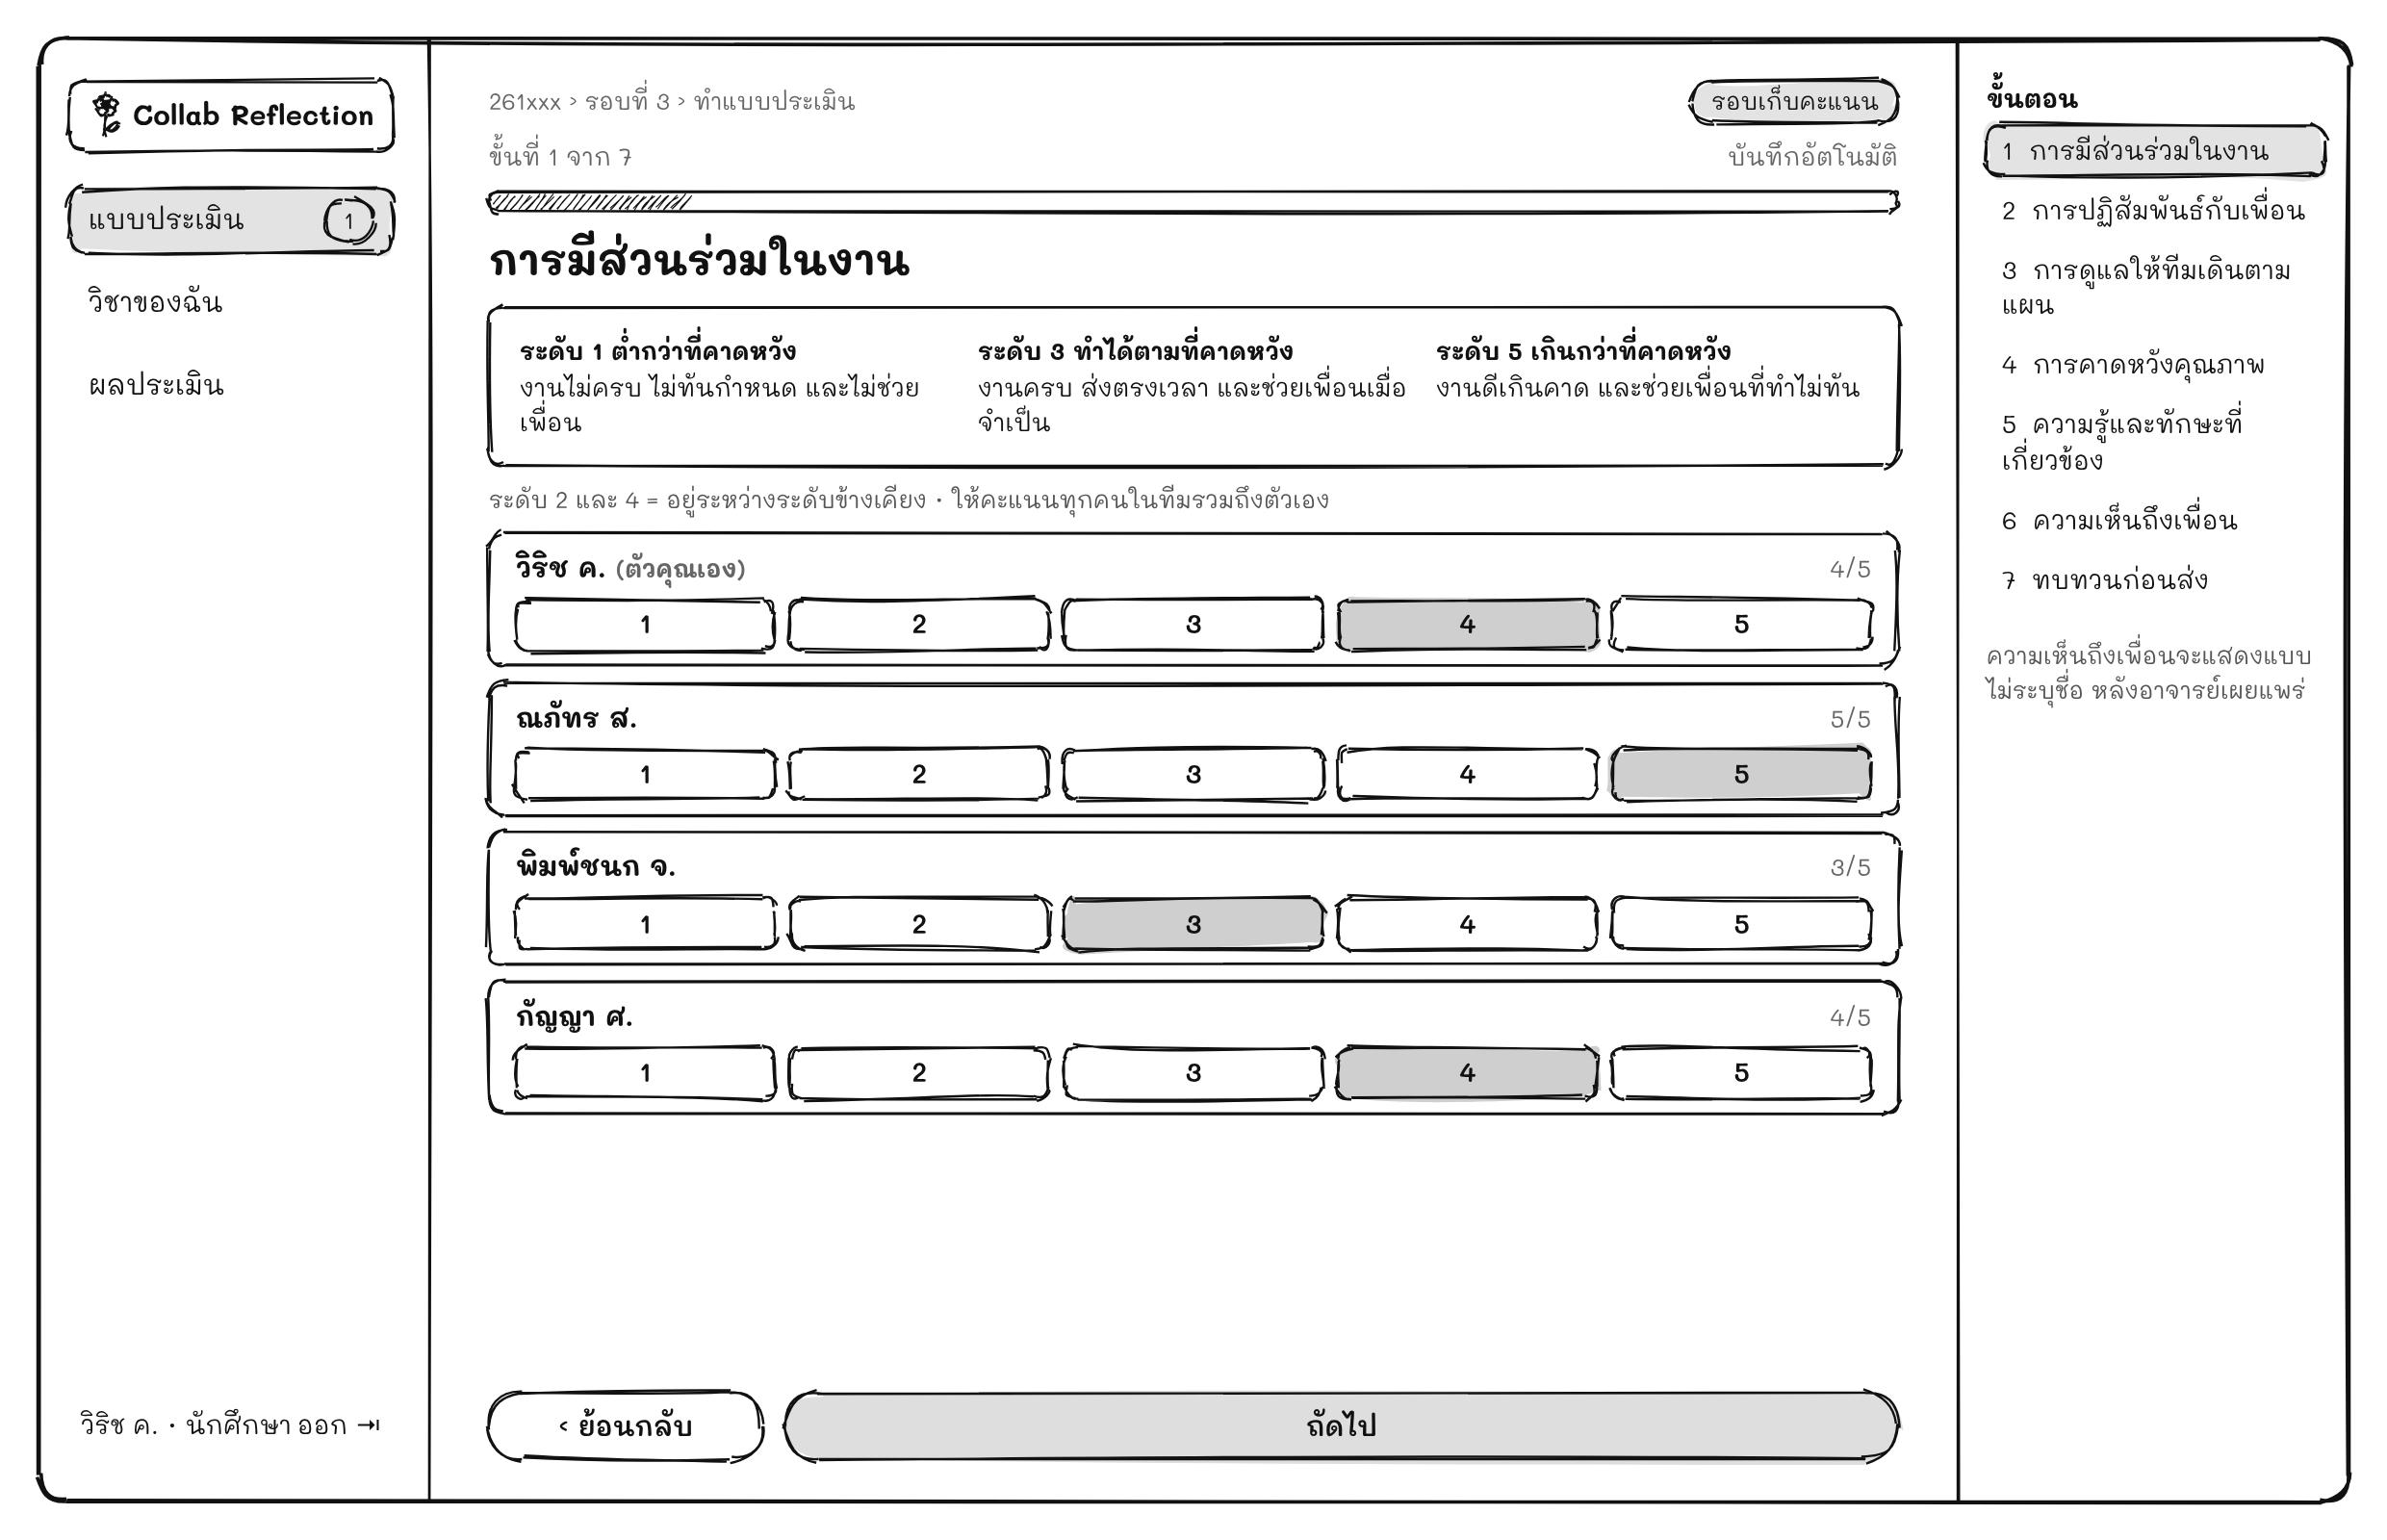
\includegraphics[width=0.85\textwidth]{figures/ch3/fig3-8-student-rating.png}}{\fbox{\parbox{0.8\textwidth}{\centering\vspace{2cm}[วางไฟล์ figures/ch3/fig3-8-student-rating.png]\vspace{2cm}}}}
\caption{หน้าให้คะแนนรายด้าน}\label{fig:ch3-8}
\end{figure}

ขั้นความเห็นถึงเพื่อนใช้แนวคิด ``ให้ดอกไม้ เติมปุ๋ย'' ดอกไม้คือสิ่งที่เพื่อนทำดีอยู่แล้วและควรได้รับคำชมเพื่อให้เติบโตต่อ ส่วนปุ๋ยเป็นสิ่งที่ช่วยให้เพื่อนเติบโตในงานถัดไป หน้าจอมีกล่องอธิบายพร้อมตัวอย่างการเขียน และภาพประกอบการเติบโตจากต้นอ่อนเป็นดอกไม้ ดังรูปที่~\ref{fig:ch3-9}

\begin{figure}[htbp]
\centering
\IfFileExists{figures/ch3/fig3-9-student-comments.png}{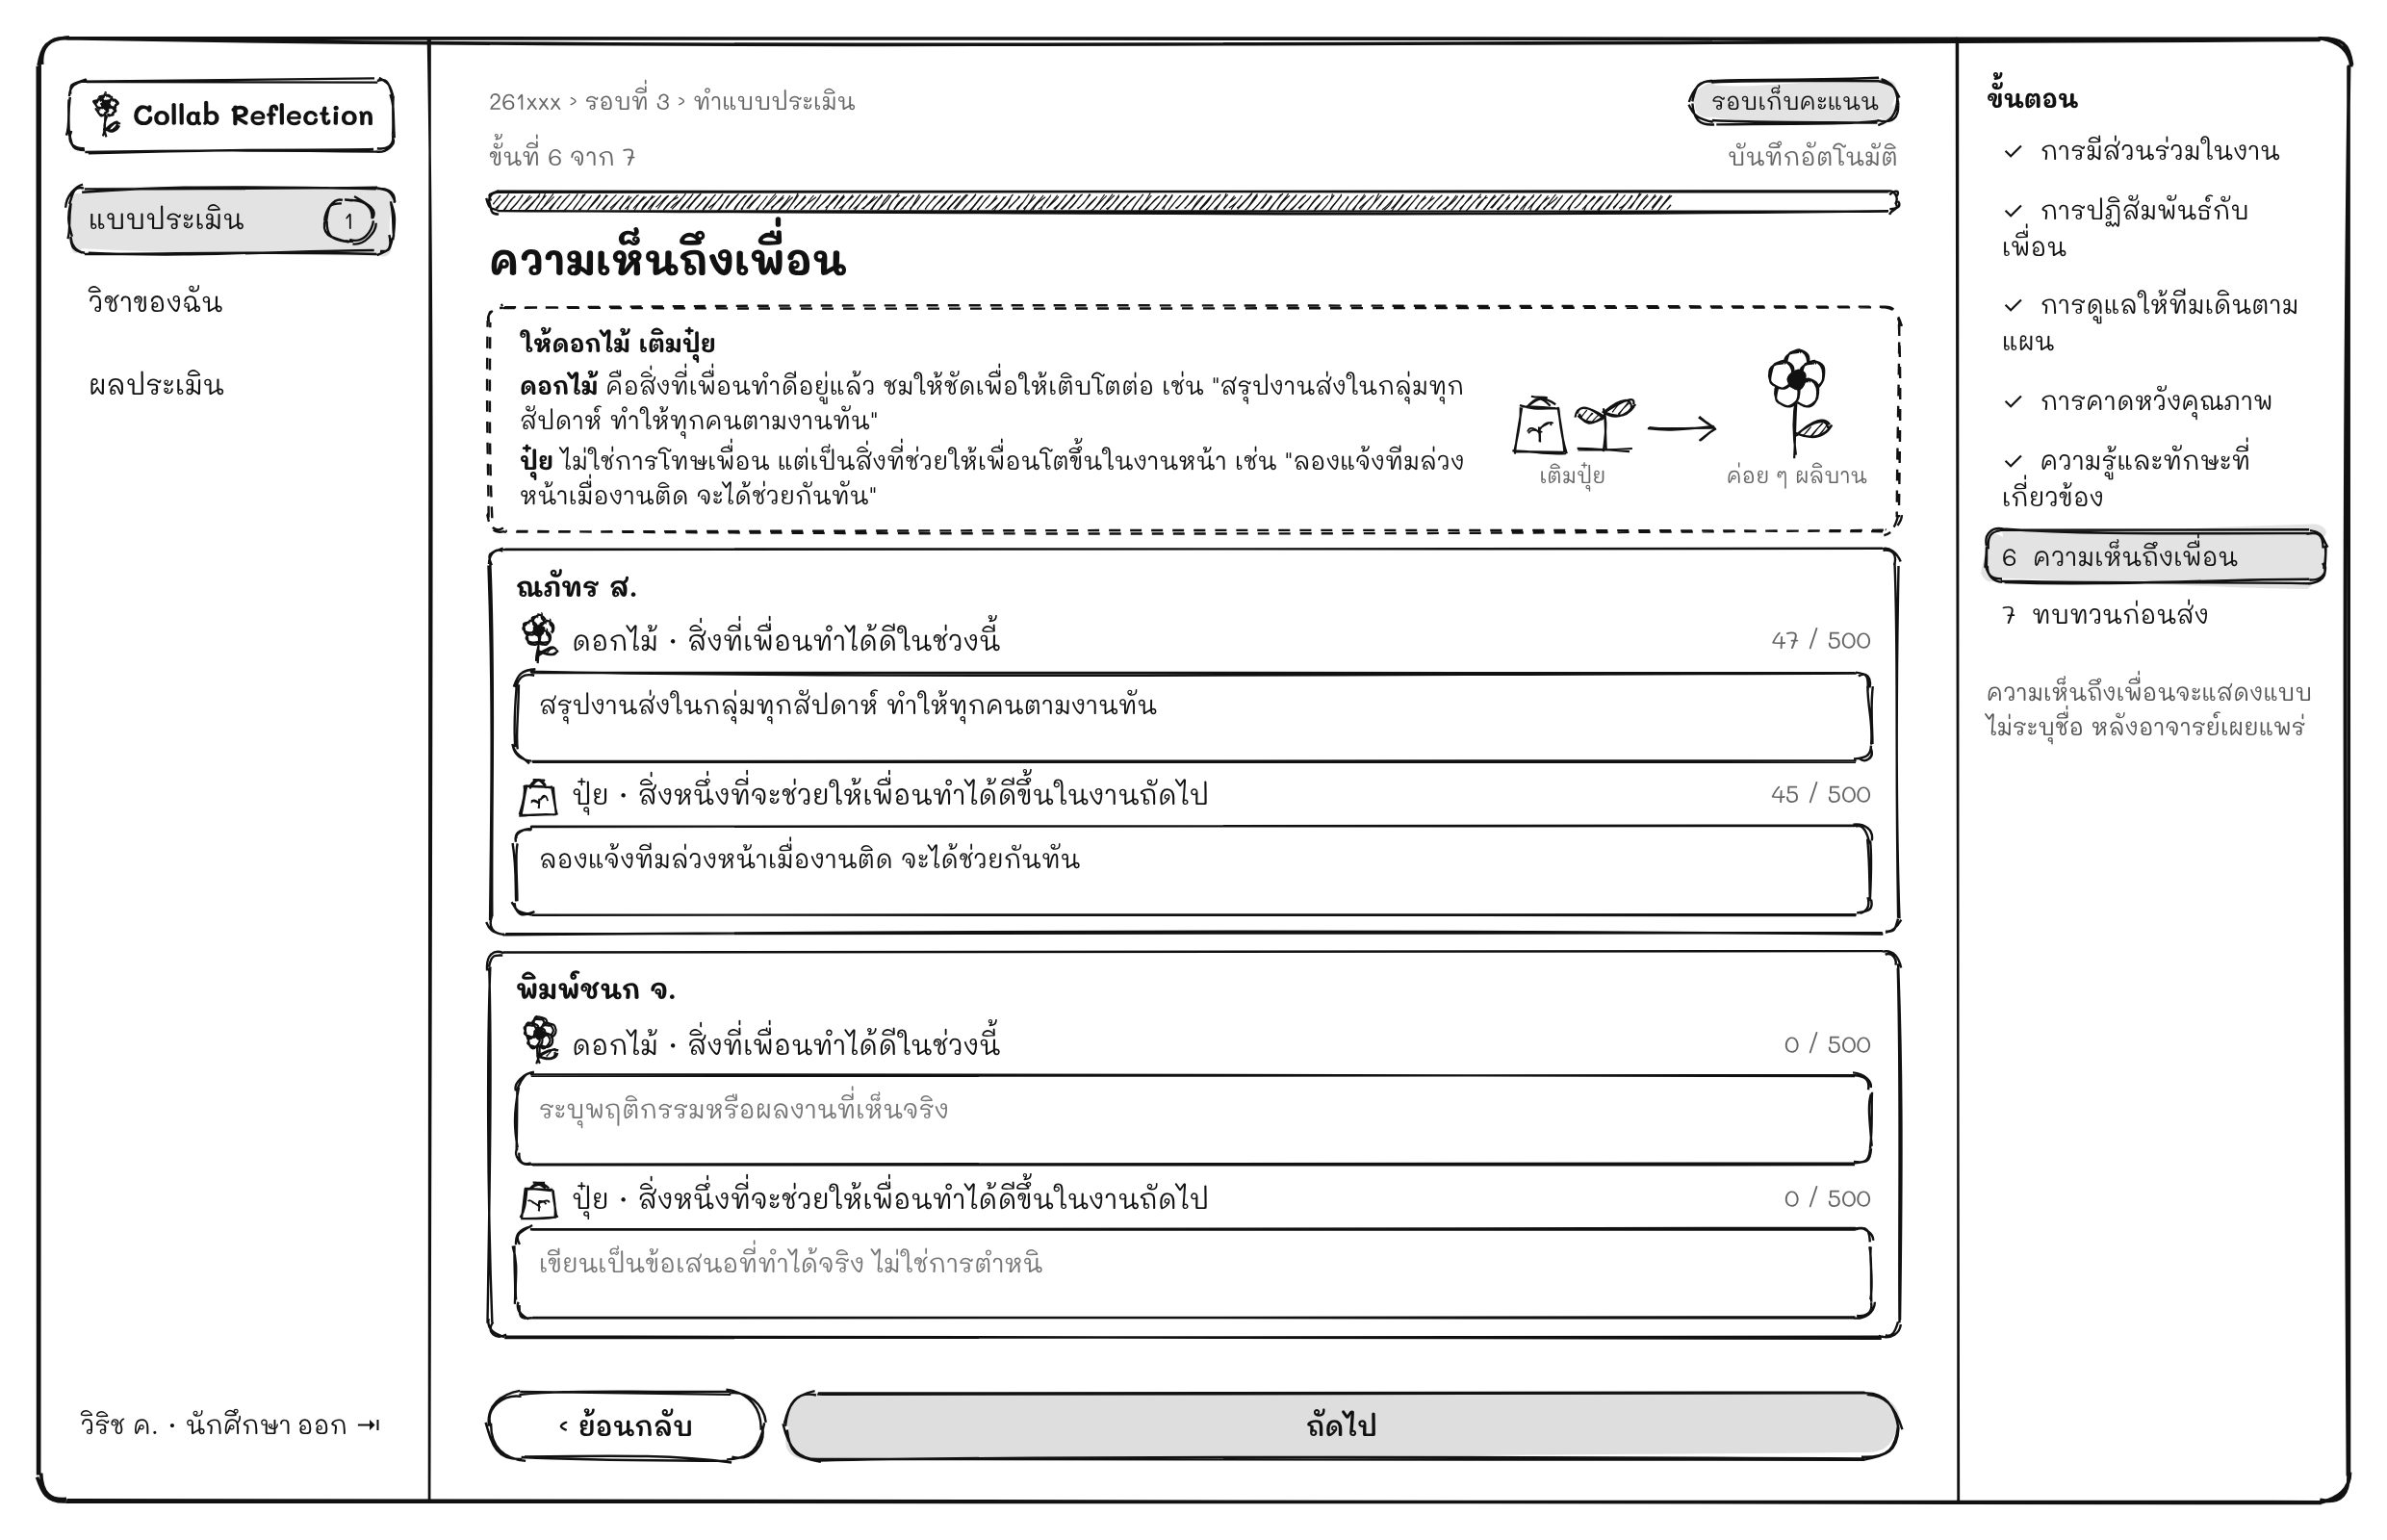
\includegraphics[width=0.85\textwidth]{figures/ch3/fig3-9-student-comments.png}}{\fbox{\parbox{0.8\textwidth}{\centering\vspace{2cm}[วางไฟล์ figures/ch3/fig3-9-student-comments.png]\vspace{2cm}}}}
\caption{หน้าเขียนความเห็นแบบดอกไม้และปุ๋ย}\label{fig:ch3-9}
\end{figure}

หน้าดูผลแสดงคะแนนรายด้านด้วยแผนภูมิเรดาร์ เปรียบเทียบค่าเฉลี่ยที่เพื่อนประเมินกับคะแนนที่ประเมินตนเอง แสดงดอกไม้และปุ๋ยที่ได้รับ ข้อเสนอแนะจากอาจารย์ และมีปุ่มขอความช่วยเหลือสำหรับนักศึกษาที่รู้สึกไม่สบายใจ ดังรูปที่~\ref{fig:ch3-10}

\begin{figure}[htbp]
\centering
\IfFileExists{figures/ch3/fig3-10-student-result.png}{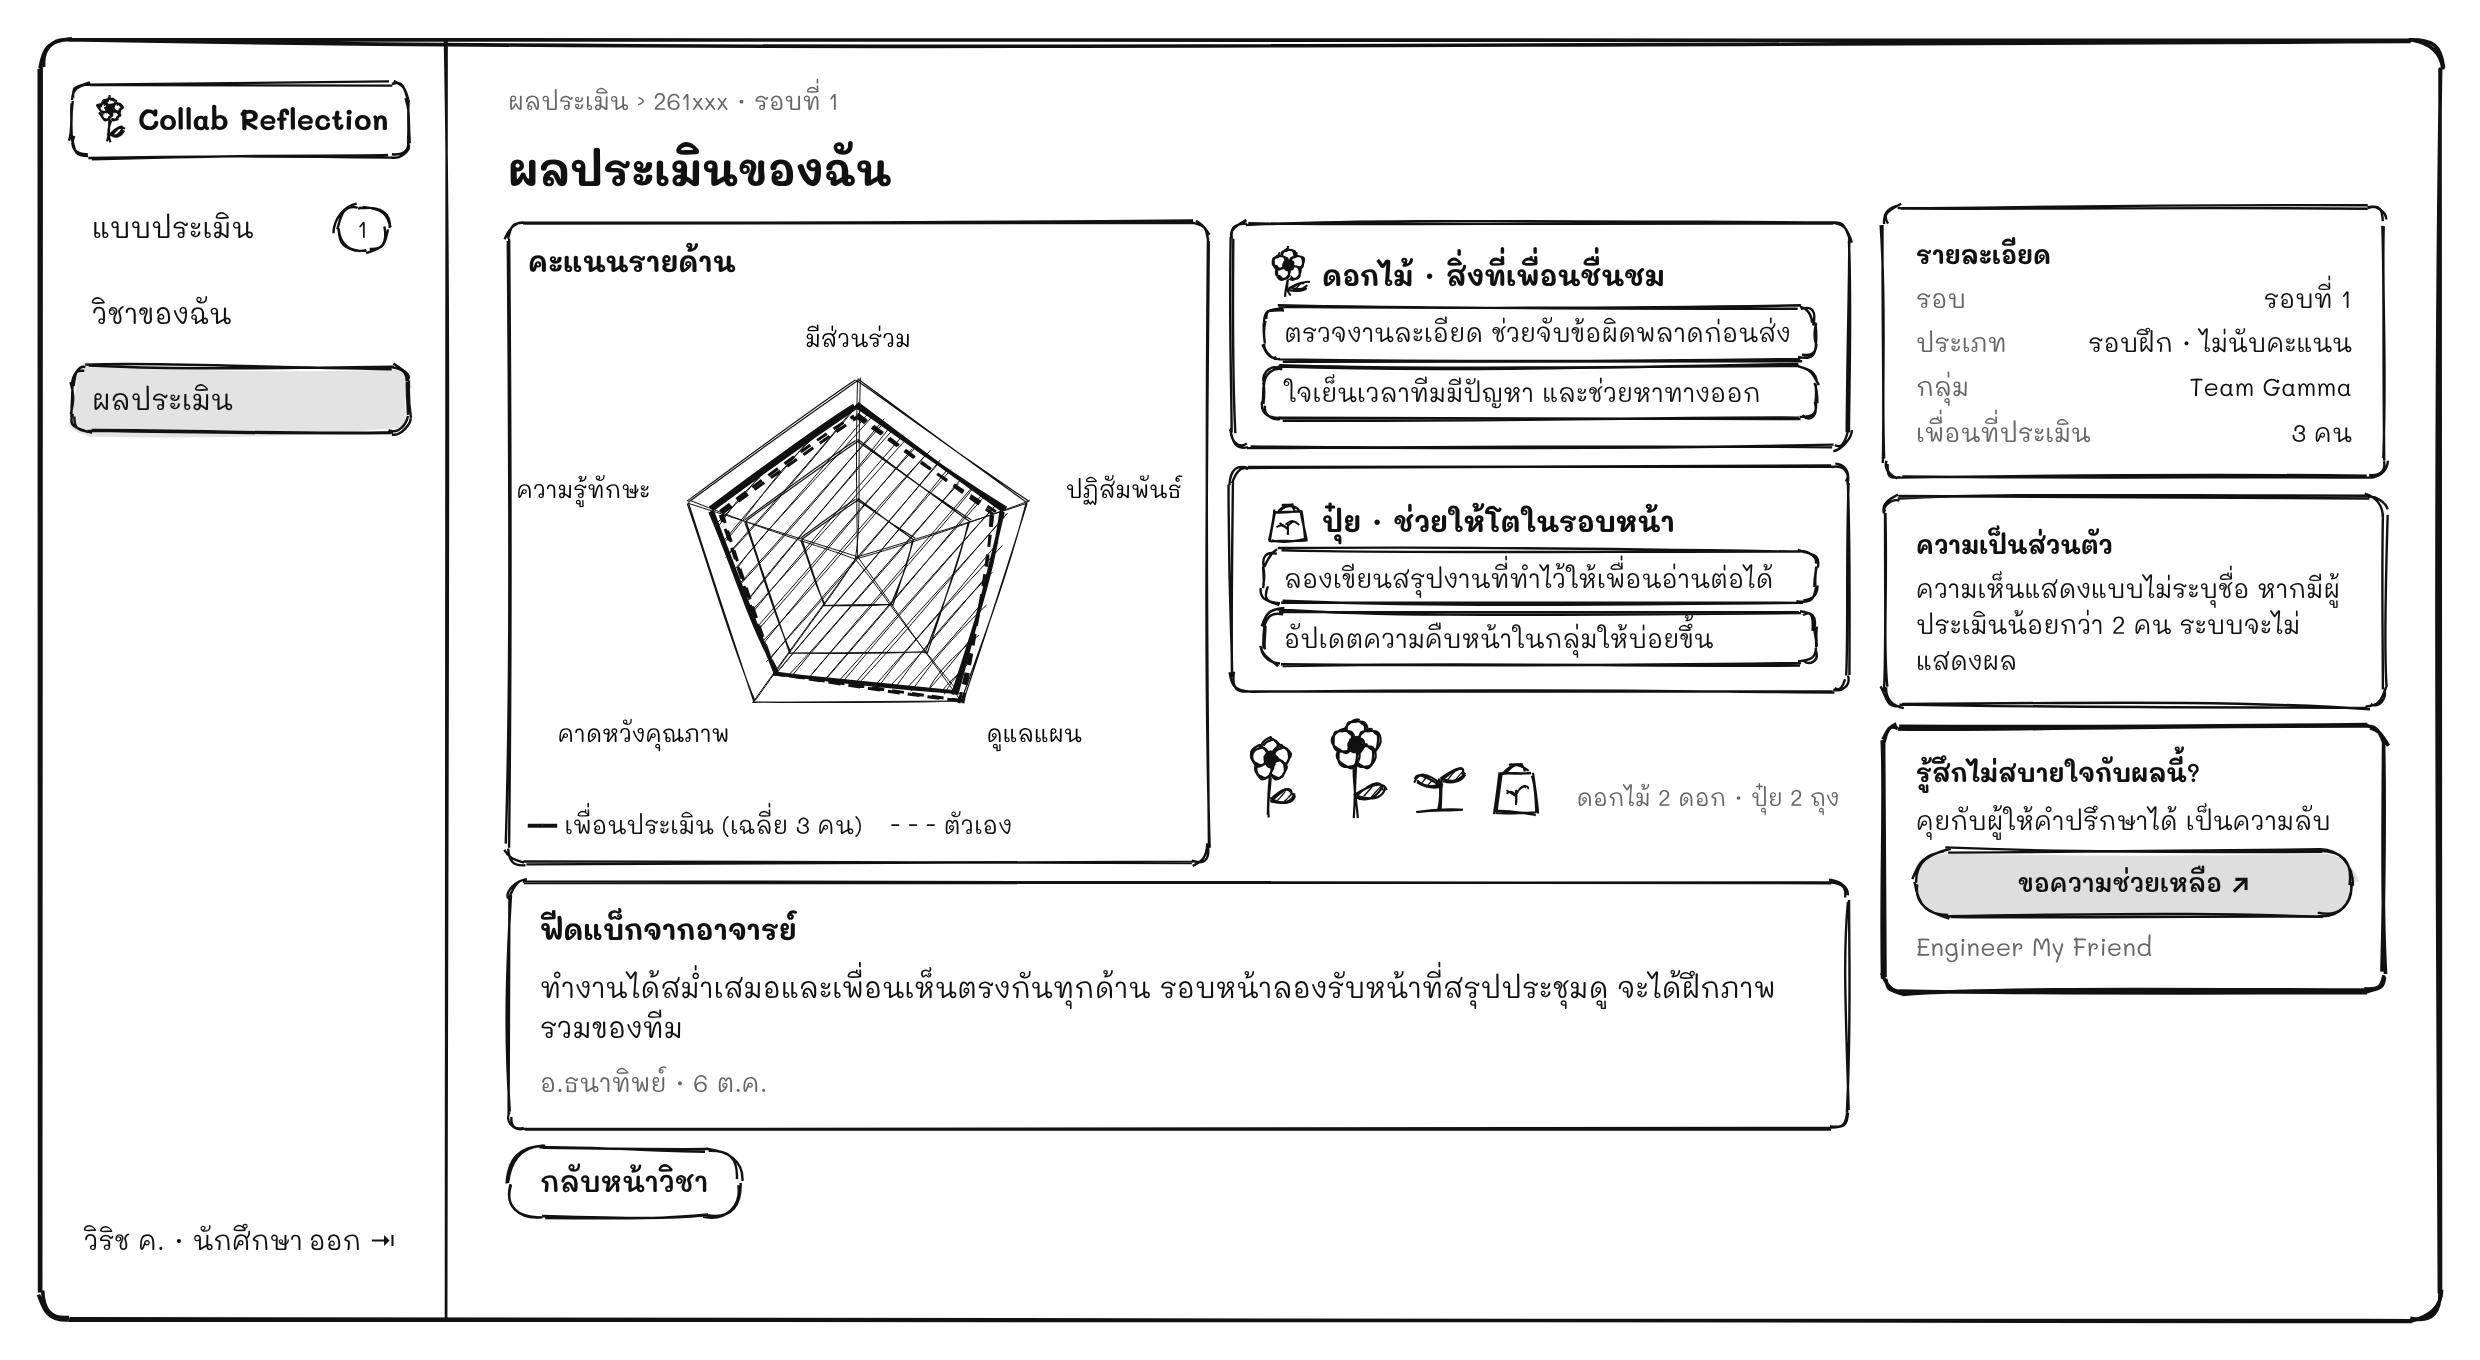
\includegraphics[width=\textwidth]{figures/ch3/fig3-10-student-result.png}}{\fbox{\parbox{0.8\textwidth}{\centering\vspace{2cm}[วางไฟล์ figures/ch3/fig3-10-student-result.png]\vspace{2cm}}}}
\caption{หน้าดูผลการประเมินของนักศึกษา}\label{fig:ch3-10}
\end{figure}

\subsection{หน้าจอฝั่งอาจารย์}\label{sec:3.8.3}

หน้าสมาชิกใช้นำเข้ารายชื่อนักศึกษาจากไฟล์ CSV จัดกลุ่ม และตรวจว่านักศึกษาคนใดยังไม่ยอมรับข้อตกลง PDPA ดังรูปที่~\ref{fig:ch3-11}

\begin{figure}[htbp]
\centering
\IfFileExists{figures/ch3/fig3-11-instructor-members.png}{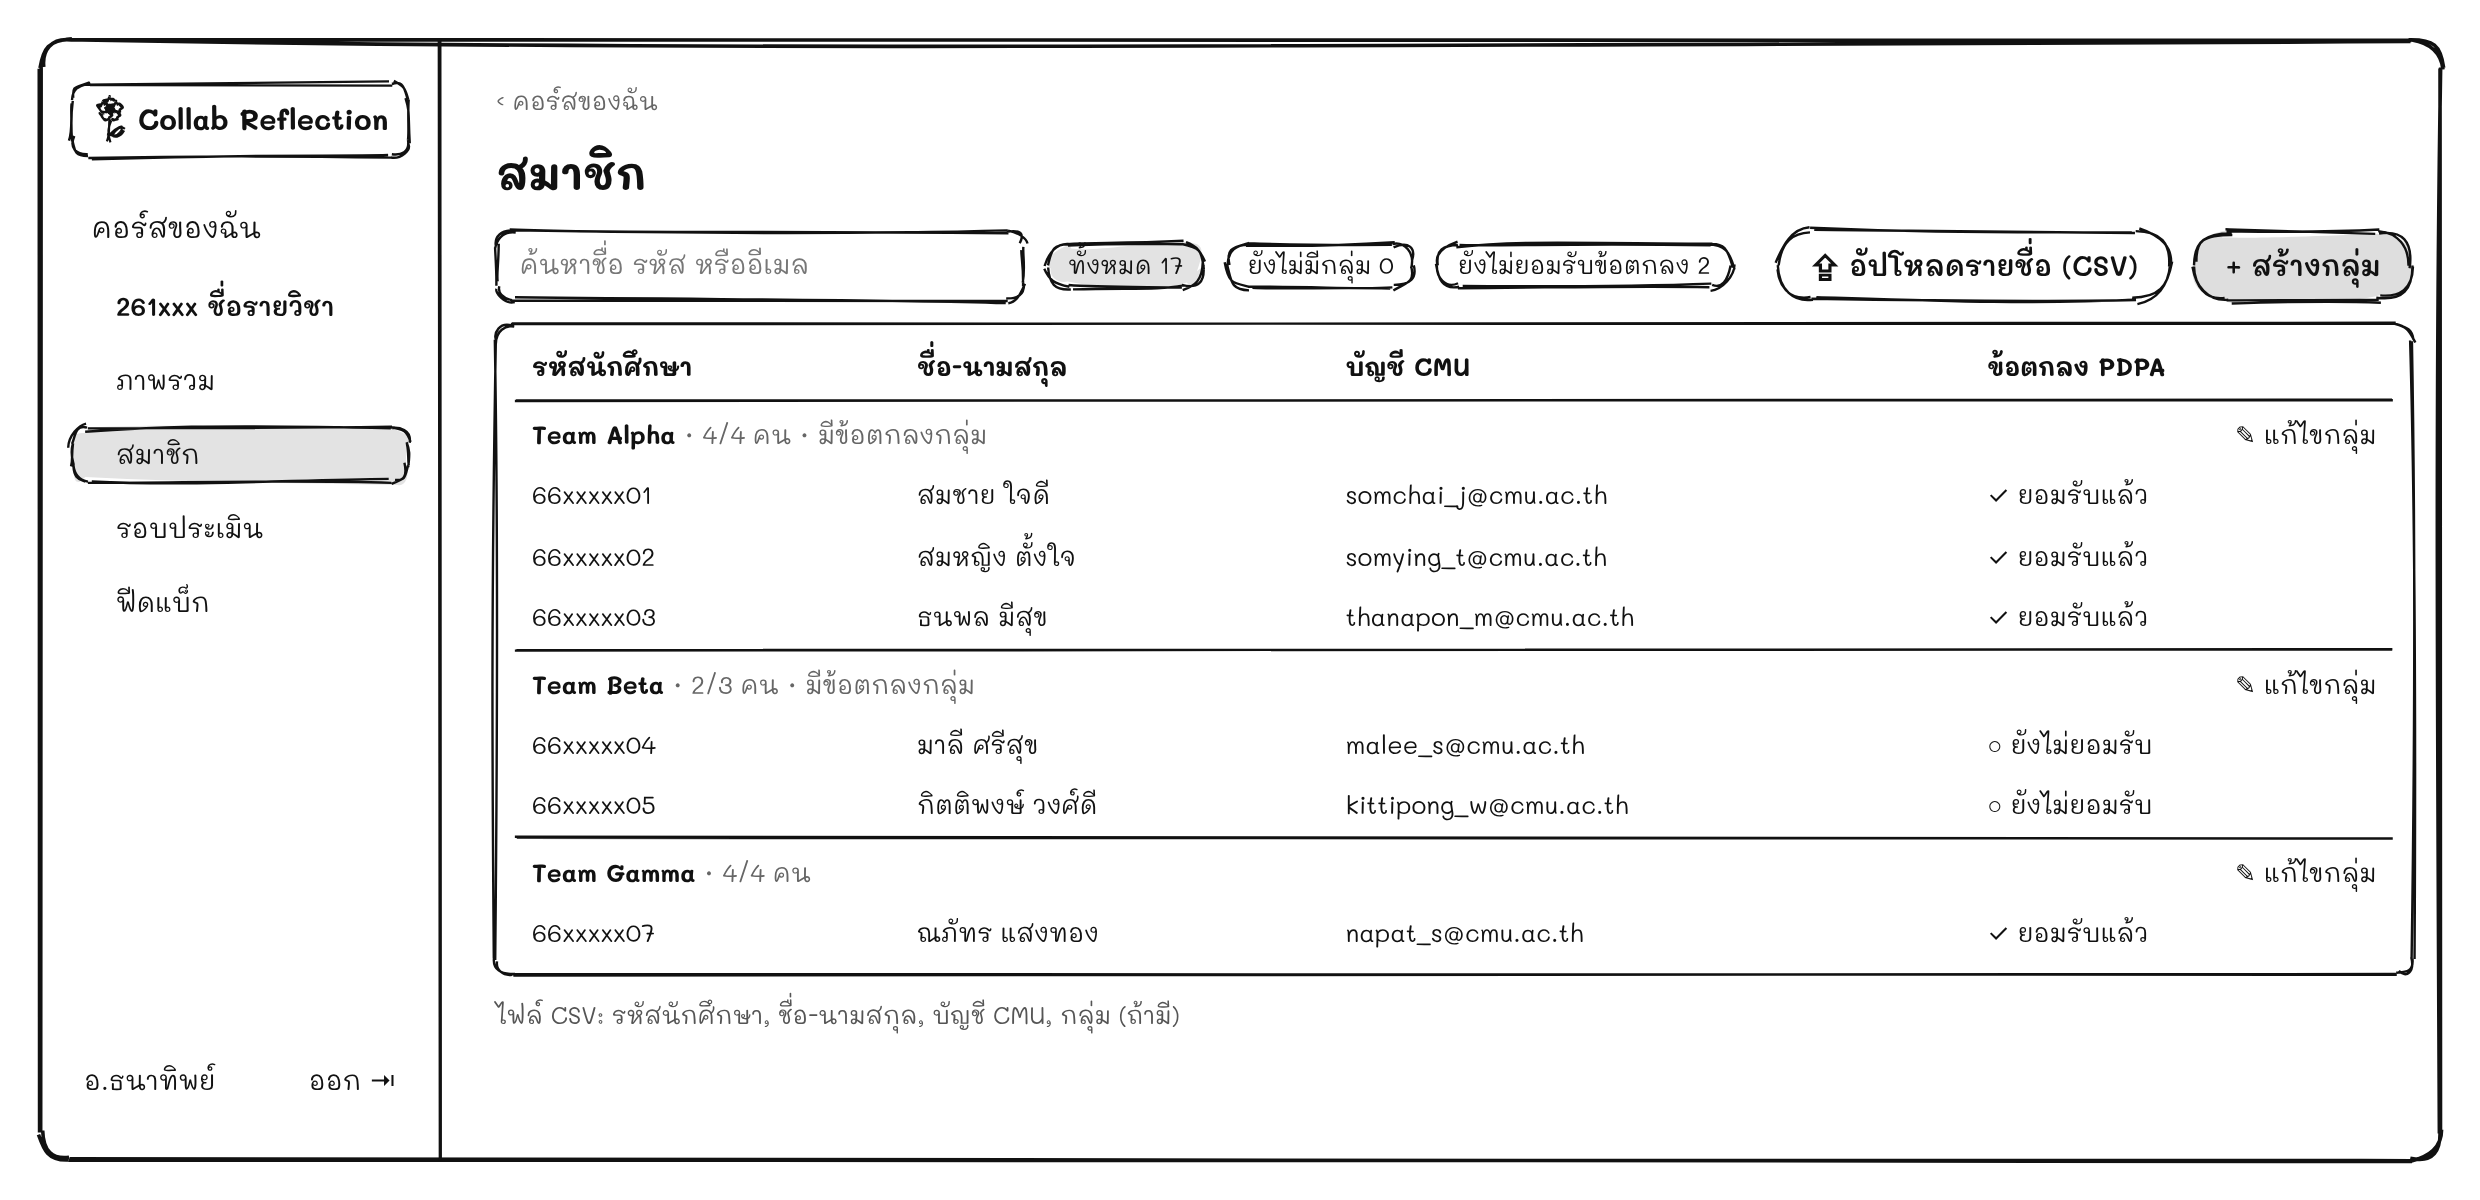
\includegraphics[width=\textwidth]{figures/ch3/fig3-11-instructor-members.png}}{\fbox{\parbox{0.8\textwidth}{\centering\vspace{2cm}[วางไฟล์ figures/ch3/fig3-11-instructor-members.png]\vspace{2cm}}}}
\caption{หน้าจัดการสมาชิกและกลุ่ม}\label{fig:ch3-11}
\end{figure}

หน้ารอบประเมินแสดงรอบทั้งหมดของรายวิชา เมื่อเพิ่มรอบใหม่ อาจารย์ต้องเลือกประเภทของรอบ (รอบฝึกหรือรอบเก็บคะแนน) และกำหนดช่วงเวลาเปิดปิด ดังรูปที่~\ref{fig:ch3-12}

\begin{figure}[htbp]
\centering
\IfFileExists{figures/ch3/fig3-12-instructor-rounds.png}{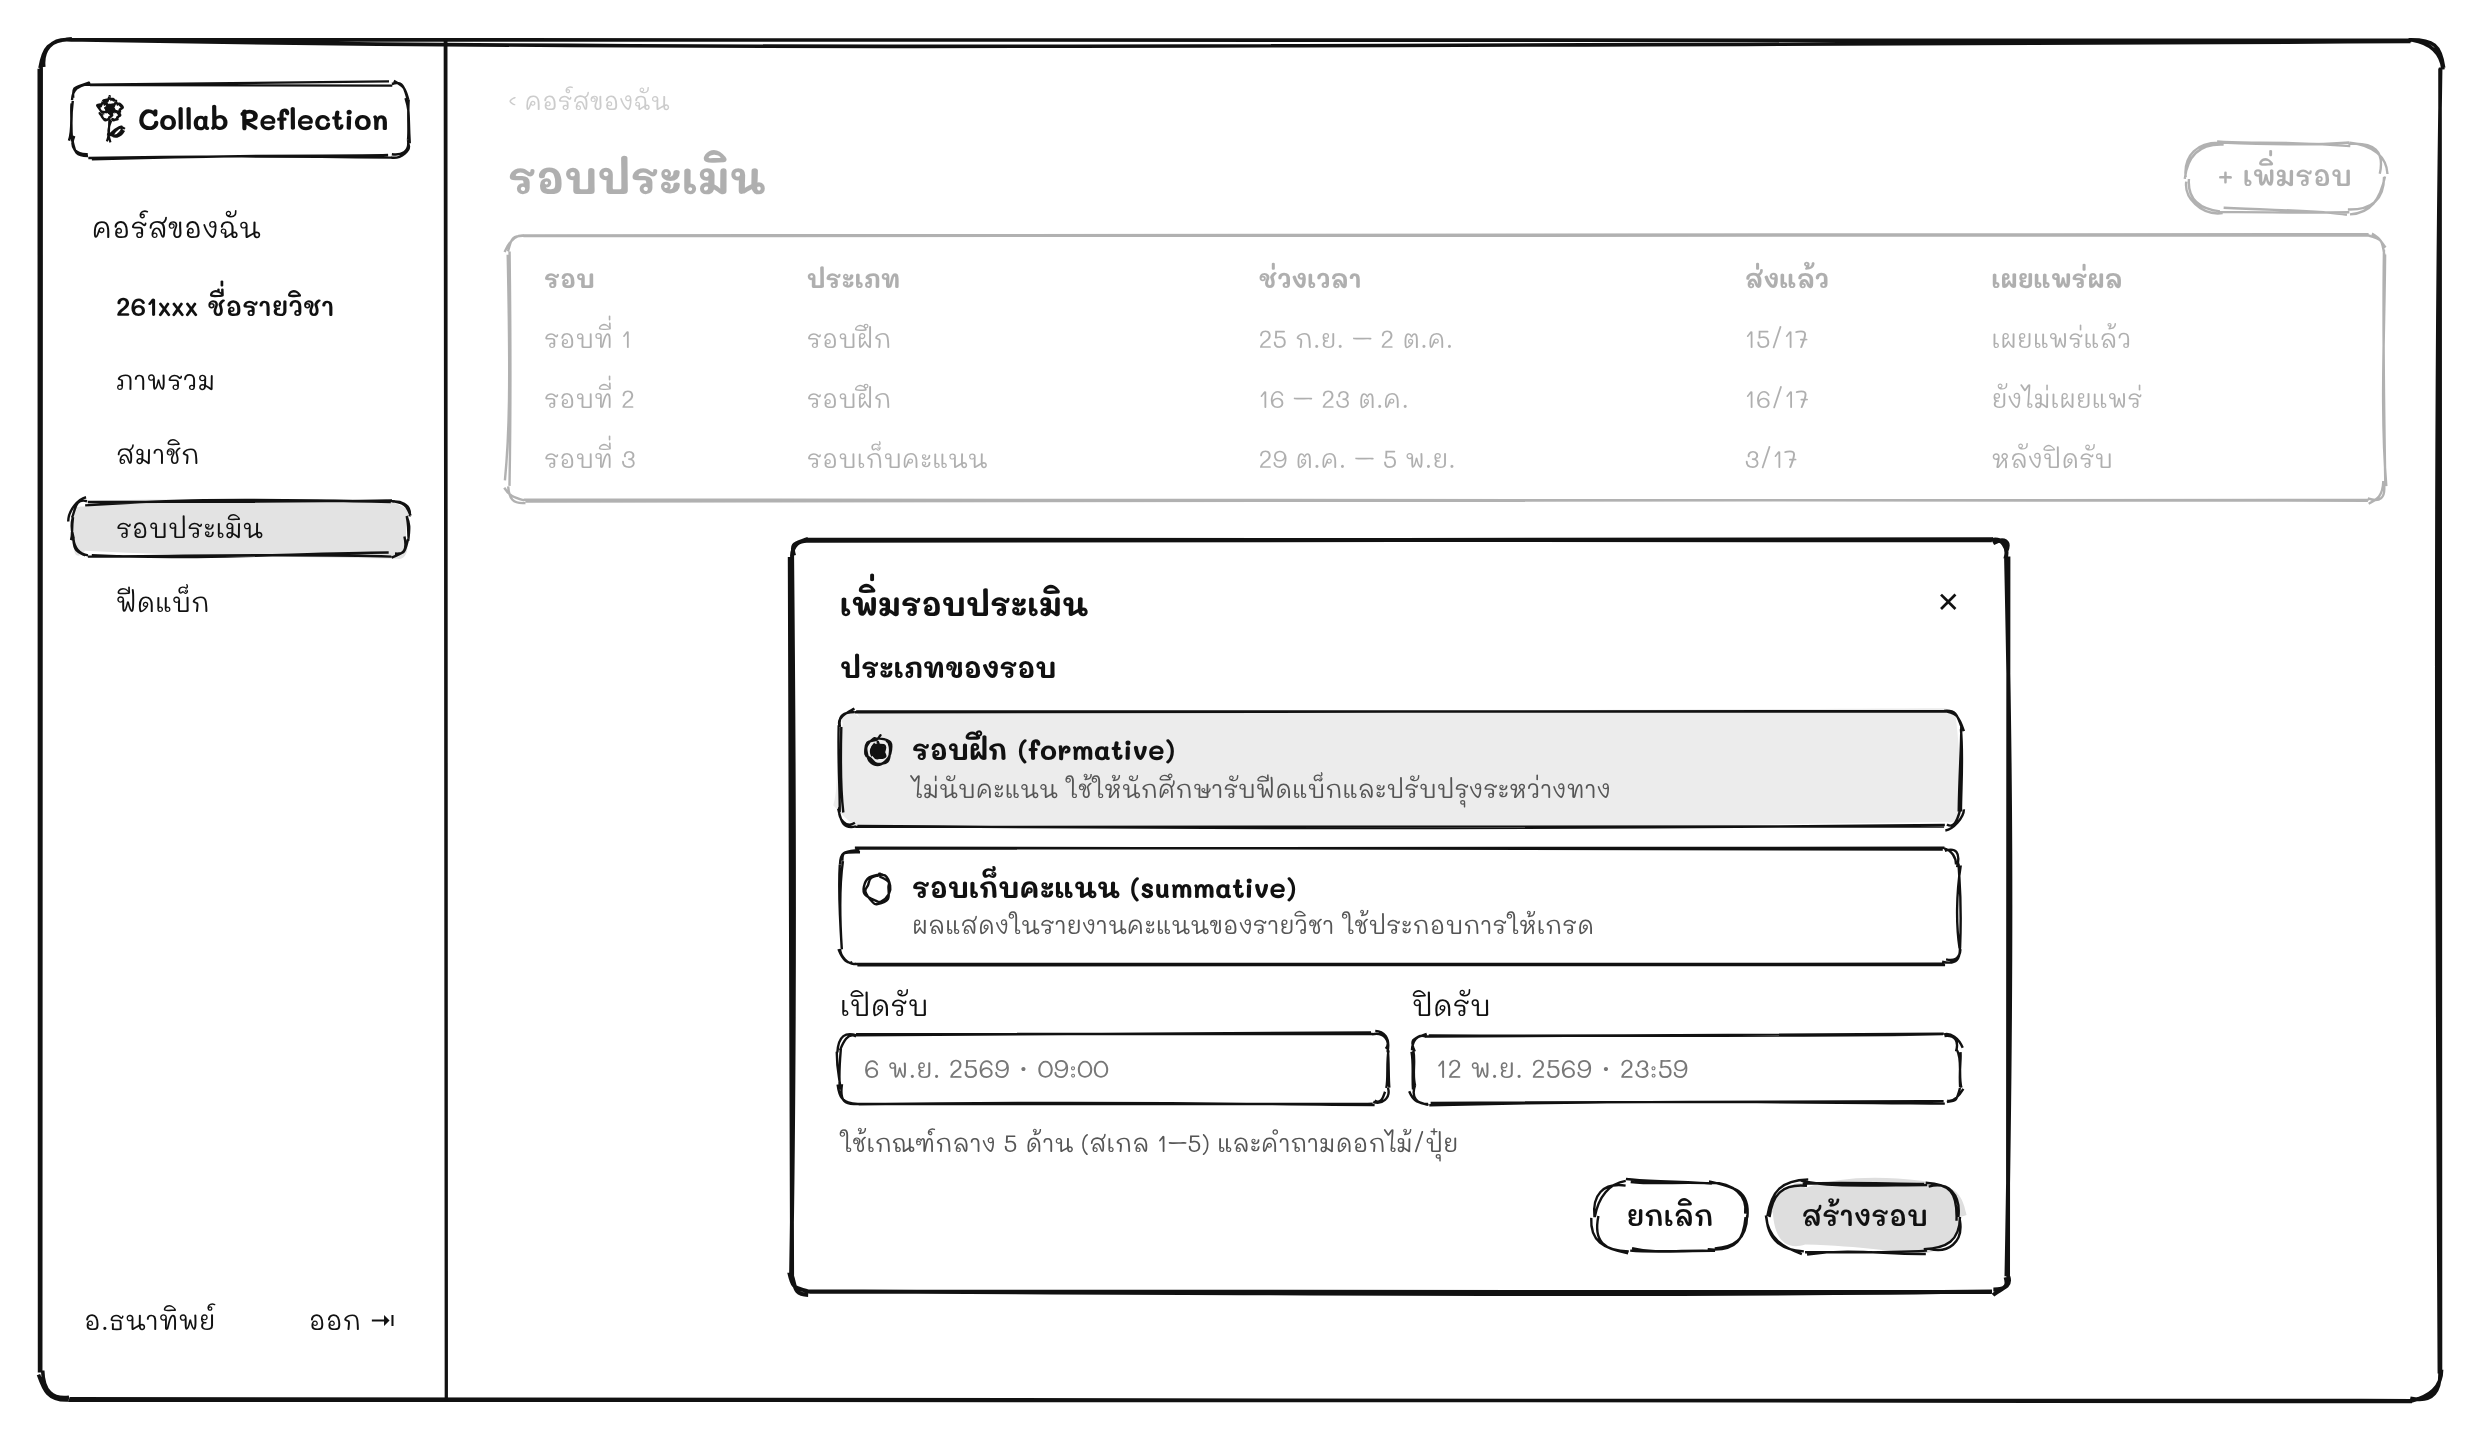
\includegraphics[width=\textwidth]{figures/ch3/fig3-12-instructor-rounds.png}}{\fbox{\parbox{0.8\textwidth}{\centering\vspace{2cm}[วางไฟล์ figures/ch3/fig3-12-instructor-rounds.png]\vspace{2cm}}}}
\caption{หน้าเพิ่มรอบประเมิน}\label{fig:ch3-12}
\end{figure}

แดชบอร์ดแสดงภาพรวมของรอบที่เลือก จำนวนผู้ส่ง แผนภาพเปรียบเทียบคะแนนที่ประเมินตนเองกับที่เพื่อนประเมิน และสัญญาณที่ควรดูของแต่ละทีม ดังรูปที่~\ref{fig:ch3-13}

\begin{figure}[htbp]
\centering
\IfFileExists{figures/ch3/fig3-13-instructor-overview.png}{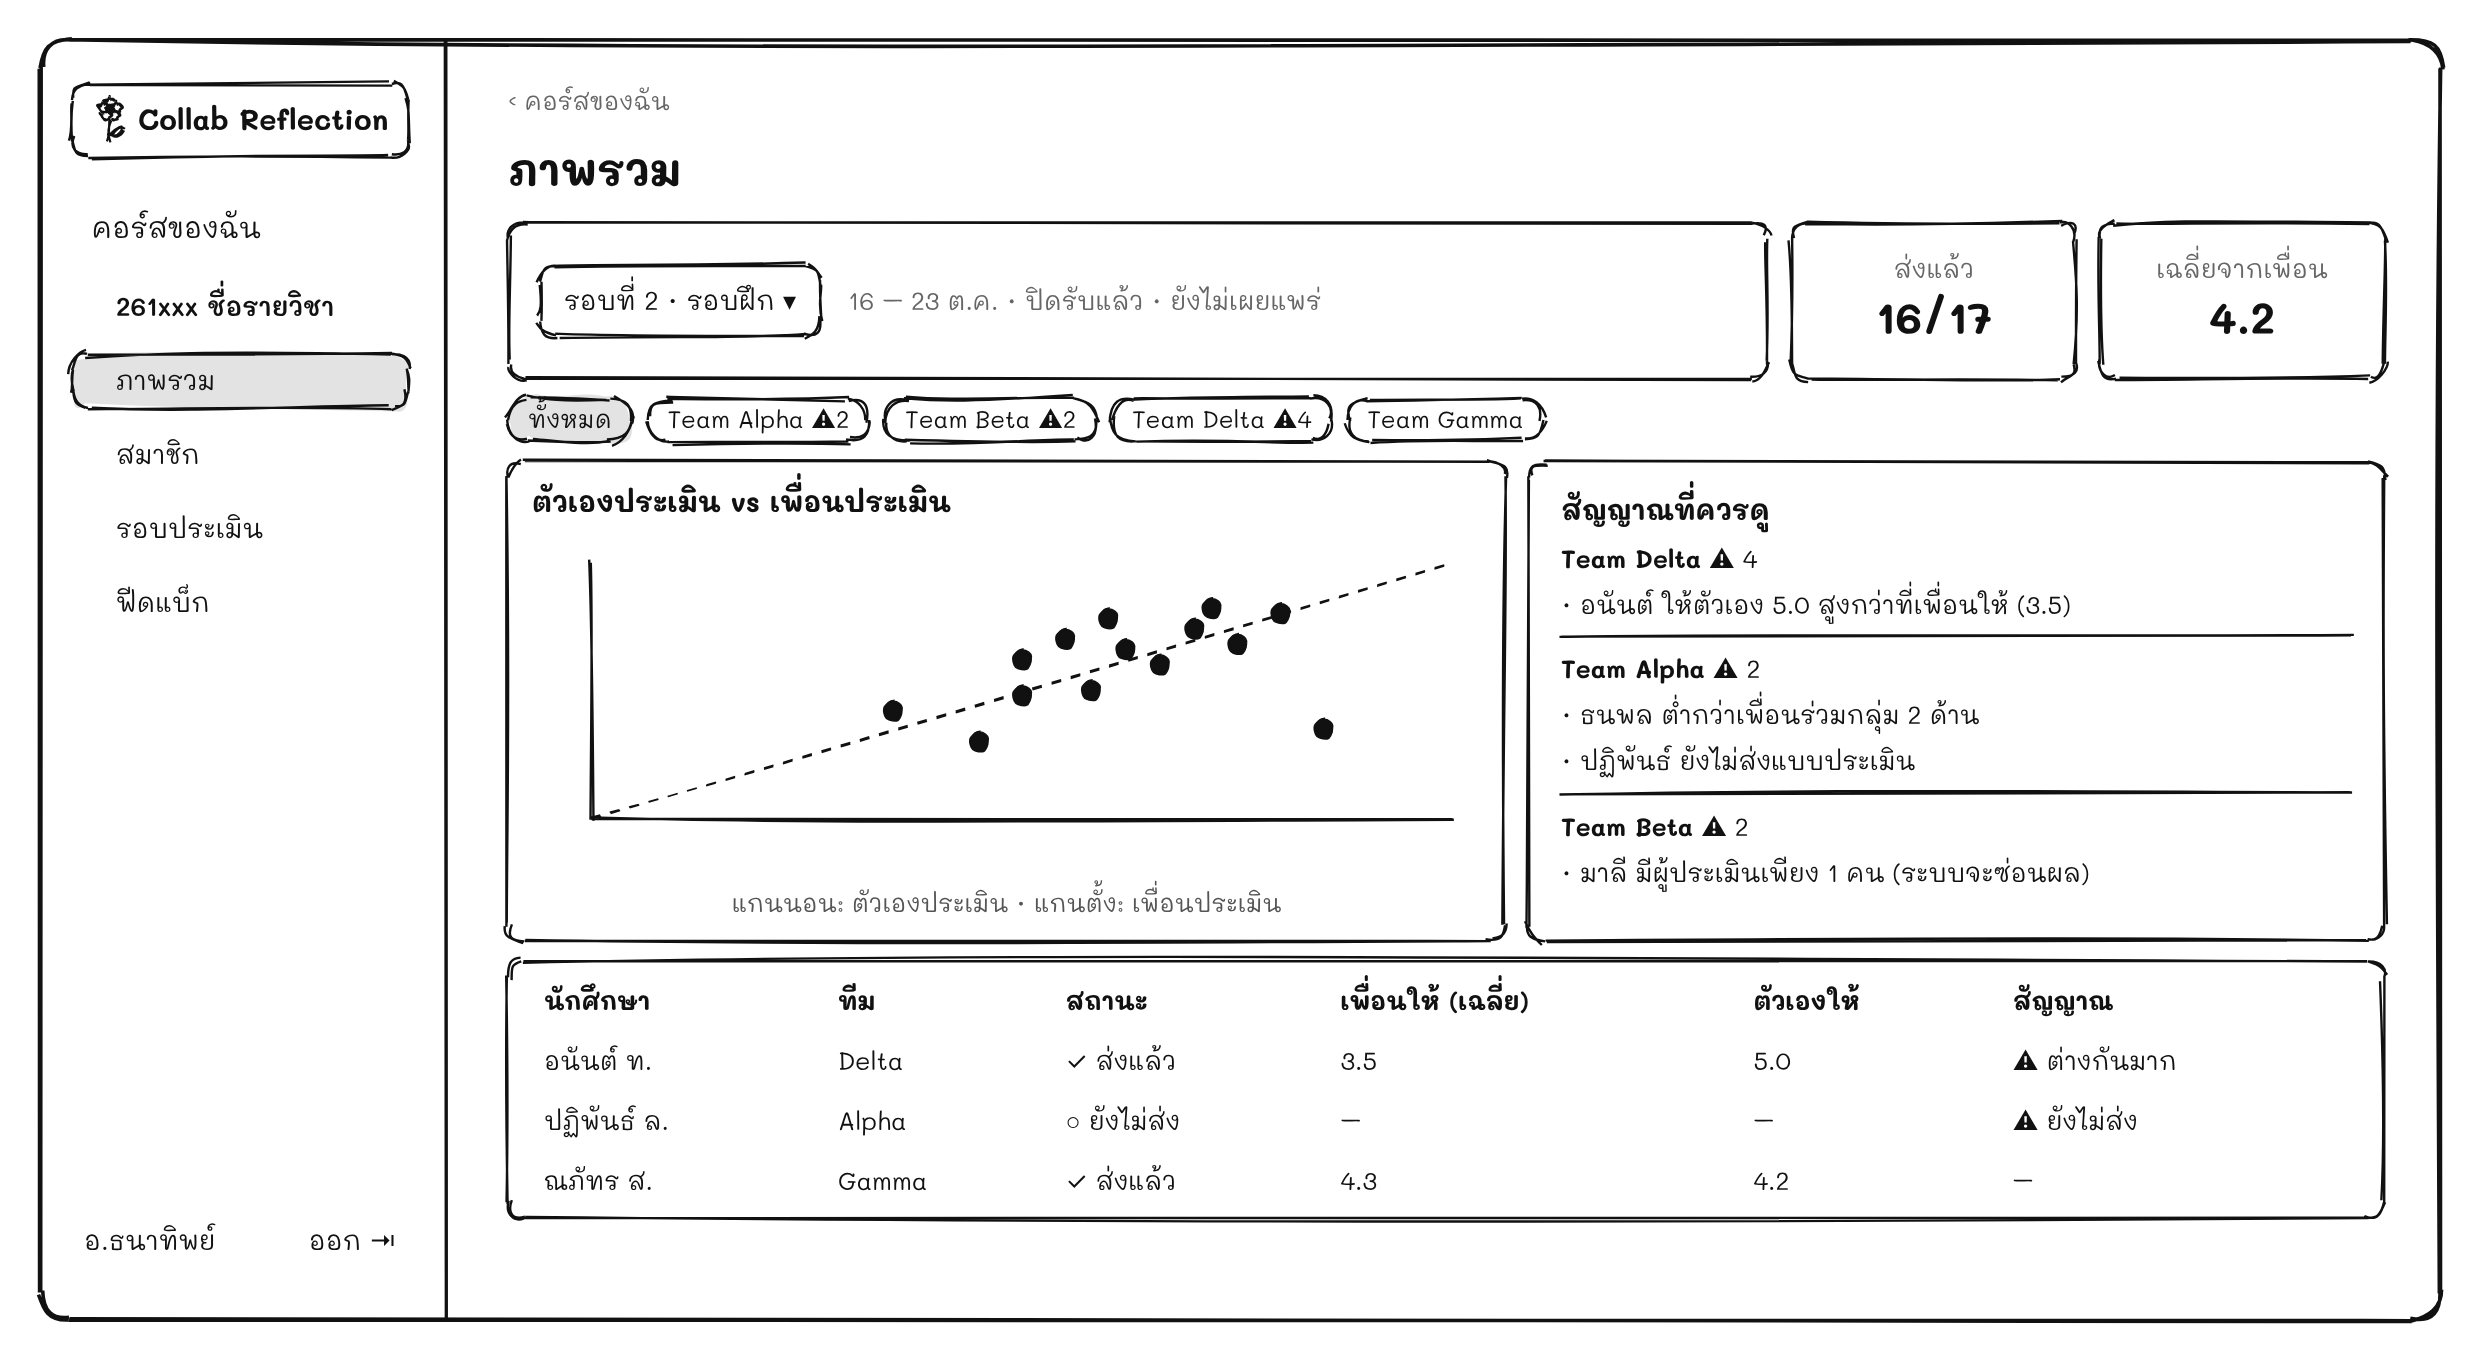
\includegraphics[width=\textwidth]{figures/ch3/fig3-13-instructor-overview.png}}{\fbox{\parbox{0.8\textwidth}{\centering\vspace{2cm}[วางไฟล์ figures/ch3/fig3-13-instructor-overview.png]\vspace{2cm}}}}
\caption{แดชบอร์ดของอาจารย์}\label{fig:ch3-13}
\end{figure}

หน้าภาพรวมแสดงผลของนักศึกษาทีละคน ให้อาจารย์อ่านดอกไม้และปุ๋ยจากเพื่อน เลือกว่านักศึกษาจะเห็นความเห็นของเพื่อนตามจริงหรือเฉพาะข้อสรุปของอาจารย์ เขียนข้อเสนอแนะ และกดเผยแพร่ผลของทั้งรอบ ดังรูปที่~\ref{fig:ch3-14}

\begin{figure}[htbp]
\centering
\IfFileExists{figures/ch3/fig3-14-instructor-feedback.png}{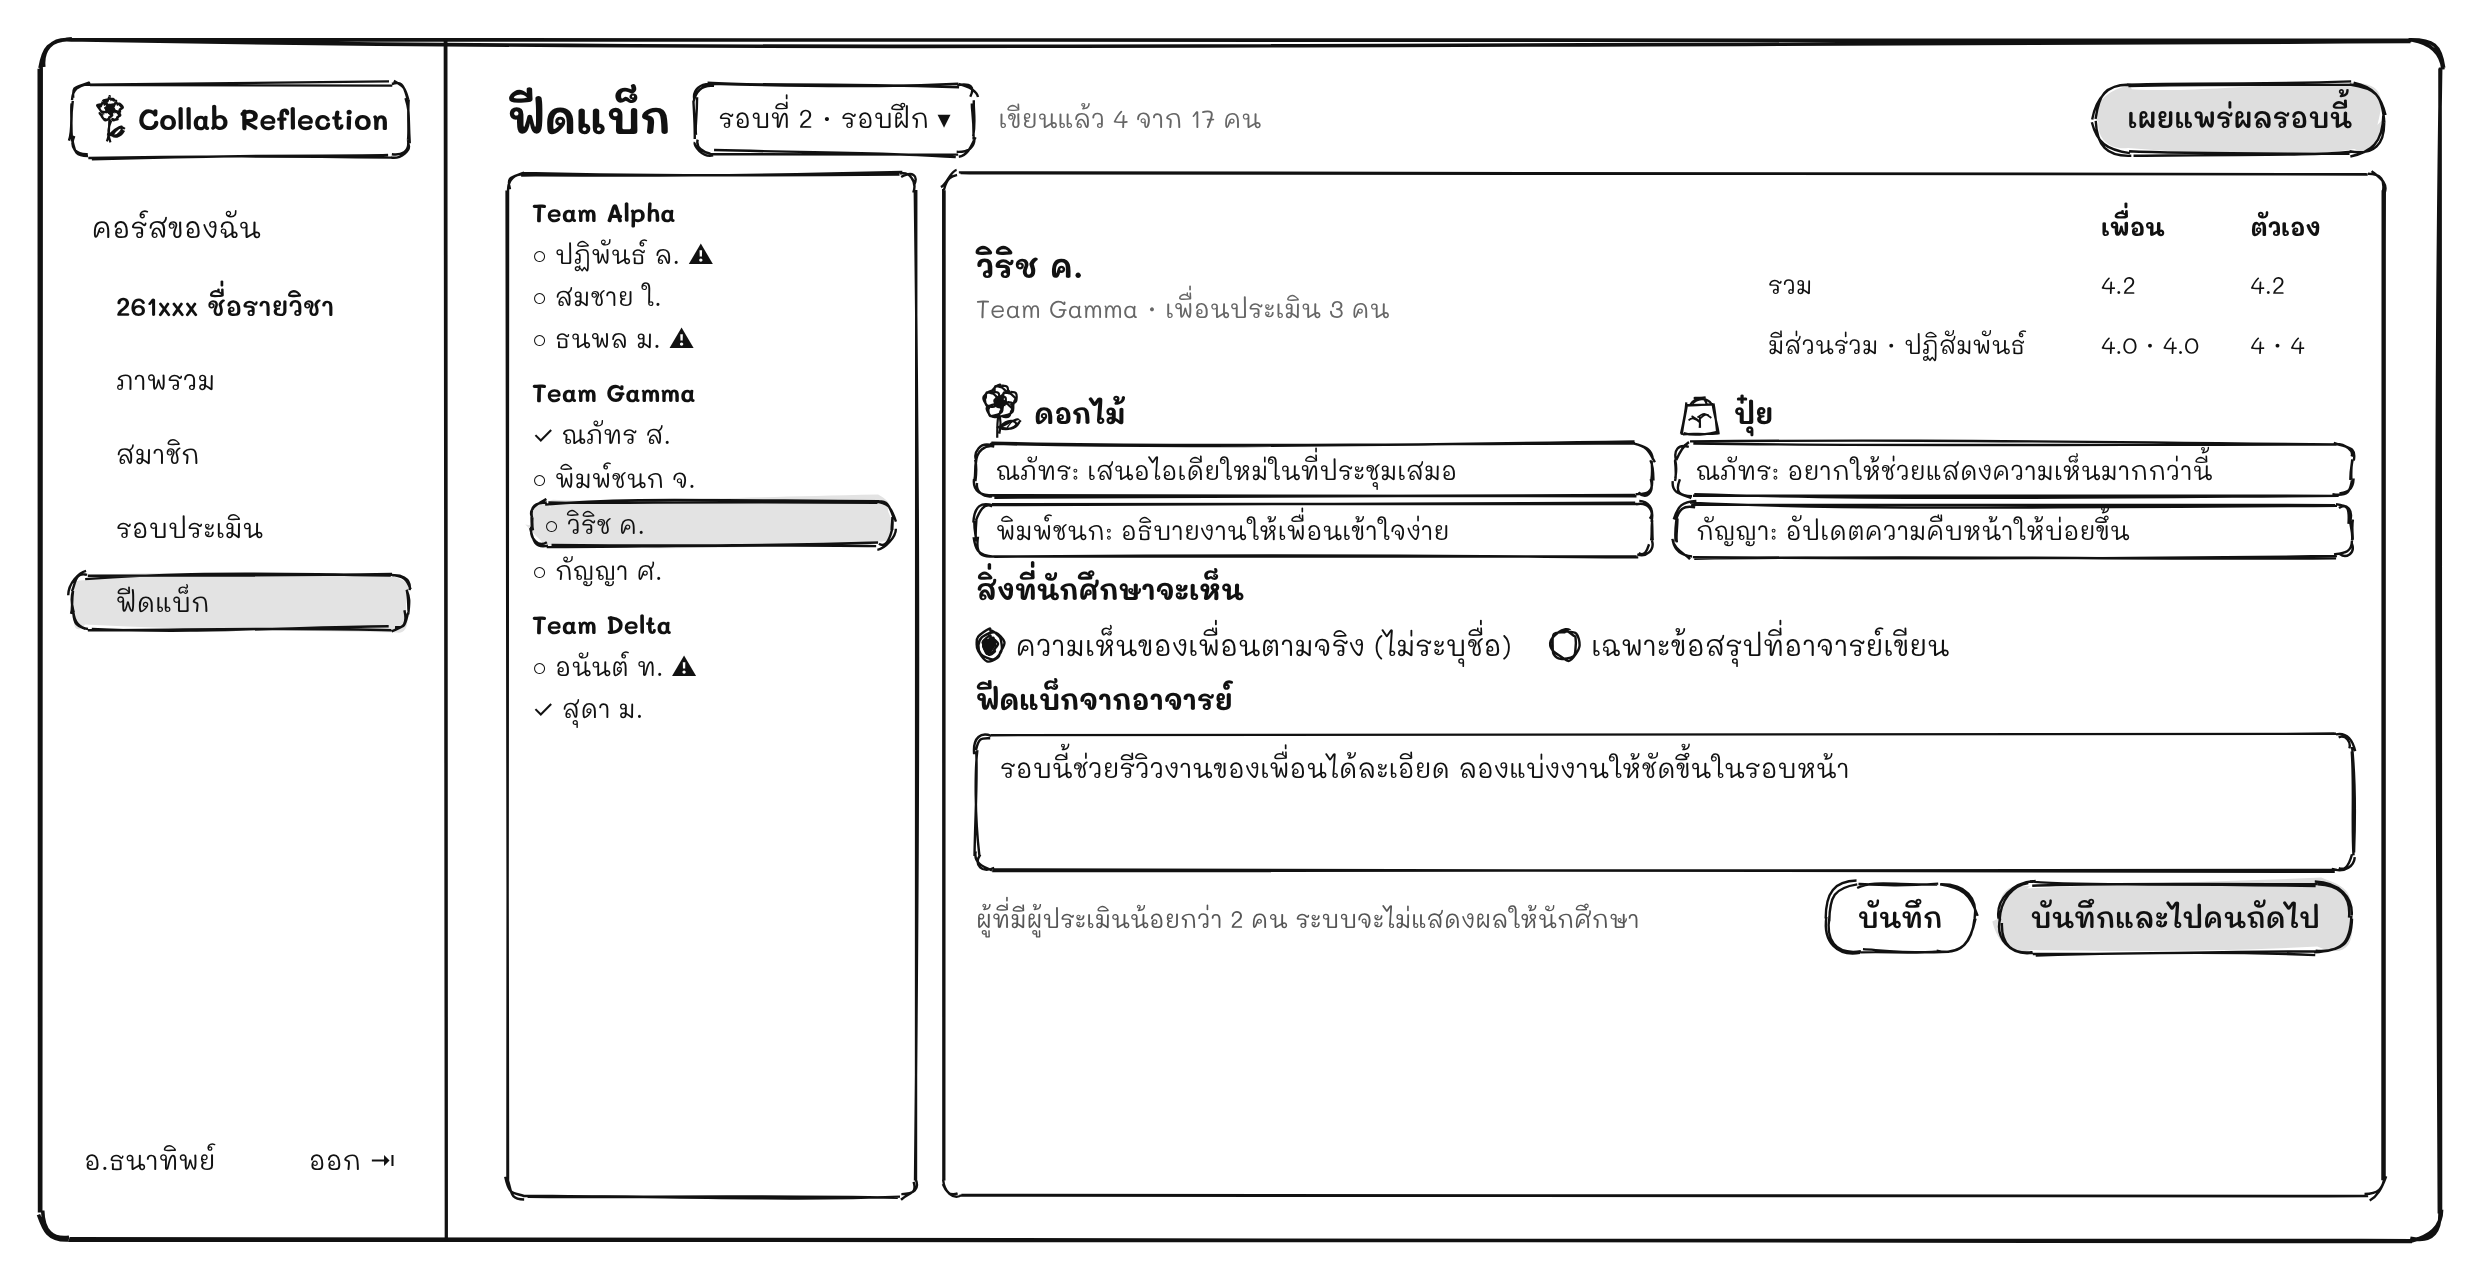
\includegraphics[width=\textwidth]{figures/ch3/fig3-14-instructor-feedback.png}}{\fbox{\parbox{0.8\textwidth}{\centering\vspace{2cm}[วางไฟล์ figures/ch3/fig3-14-instructor-feedback.png]\vspace{2cm}}}}
\caption{หน้าตรวจทานและเผยแพร่ผล}\label{fig:ch3-14}
\end{figure}

\section{ความปลอดภัยและการคุ้มครองข้อมูลส่วนบุคคล}\label{sec:3.9}

\subsection{ความปลอดภัยของระบบ}\label{sec:3.9.1}

\begin{itemize}
  \item เข้าสู่ระบบด้วยบัญชี CMU เท่านั้น และระบบไม่เก็บรหัสผ่าน
  \item ตรวจสิทธิ์ตามบทบาทในทุก API และบังคับกฎการปกปิดตัวตนที่ฝั่งเซิร์ฟเวอร์
  \item เข้ารหัสการสื่อสารด้วย HTTPS และใช้คุกกี้เซสชันแบบ HttpOnly และ Secure
  \item ตรวจสอบข้อมูลขาเข้าทุกครั้ง และใช้ ORM ที่สร้างคำสั่ง SQL แบบมีพารามิเตอร์ เพื่อป้องกัน SQL injection
  \item แบบประเมินที่ส่งแล้วแก้ไขไม่ได้ เพื่อป้องกันการเปลี่ยนคะแนนย้อนหลัง
\end{itemize}

\subsection{การคุ้มครองข้อมูลส่วนบุคคล}\label{sec:3.9.2}

ระบบออกแบบตามหลักของพระราชบัญญัติคุ้มครองข้อมูลส่วนบุคคล พ.ศ. 2562~\cite{pdpa2562} ได้แก่ เก็บข้อมูลเท่าที่จำเป็นต่อการประเมินงานกลุ่มเท่านั้น แจ้งก่อนใช้ว่าเก็บข้อมูลอะไร ใครเห็น และเก็บนานเท่าใด และให้เจ้าของข้อมูลใช้สิทธิ์ขอดู แก้ไข หรือลบข้อมูลได้

เพื่อไม่ให้นักศึกษาที่ไม่ยินยอมบางเรื่องต้องหลุดออกจากระบบจนเก็บคะแนนไม่ได้ ข้อตกลงจึงแบ่งเป็นส่วนจำเป็นและส่วนทางเลือก ดังตารางที่~\ref{tab:ch3-9} ทั้งนี้ คณะผู้จัดทำจะยืนยันระยะเวลาเก็บข้อมูลและฐานทางกฎหมายของการประมวลผลส่วนจำเป็นกับหน่วยงานที่ดูแลการคุ้มครองข้อมูลส่วนบุคคลของมหาวิทยาลัยก่อนใช้งานจริง

\begin{xltabular}{\textwidth}{|P{0.14\textwidth}|Y|Y|}
\caption{การแบ่งข้อตกลงการใช้ข้อมูลส่วนบุคคล}\label{tab:ch3-9}\\
\hline \textbf{ส่วน} & \textbf{ข้อมูลและการใช้งาน} & \textbf{หากไม่ยินยอม} \\ \hline
\endfirsthead
\multicolumn{3}{r}{\small (ต่อ)}\\ \hline \textbf{ส่วน} & \textbf{ข้อมูลและการใช้งาน} & \textbf{หากไม่ยินยอม} \\ \hline
\endhead
ส่วนจำเป็น & ข้อมูลบัญชี CMU รายวิชาและกลุ่มที่สังกัด คะแนนและความเห็นที่ใช้ในการประเมินของรายวิชา & ต้องรับทราบจึงจะใช้ระบบได้ เพราะเป็นข้อมูลขั้นต่ำของการประเมิน \\ \hline
ส่วนทางเลือก 1 & ส่งข้อความที่เขียนให้ปัญญาประดิษฐ์ (AI) ประมวลผล (เฟสที่ 2) & ใช้ระบบและได้คะแนนตามปกติ แต่ข้อความของผู้นั้นจะไม่ถูกส่งให้ปัญญาประดิษฐ์ (AI) \\ \hline
ส่วนทางเลือก 2 & นำข้อมูลแบบไม่ระบุตัวตนไปใช้พัฒนาระบบและในงานวิจัย & ใช้ระบบและได้คะแนนตามปกติ แต่ข้อมูลของผู้นั้นจะไม่ถูกนำไปใช้ \\ \hline
\end{xltabular}

\subsection{การดูแลความรู้สึกของผู้ใช้}\label{sec:3.9.3}

ข้อเสนอแนะจากเพื่อนอาจกระทบความรู้สึกของผู้รับได้แม้ผ่านการกลั่นกรองแล้ว ระบบจึงลดโอกาสเกิดความคิดเห็นที่ทำร้ายจิตใจตั้งแต่ต้นทาง ด้วยคำถามแบบดอกไม้และปุ๋ย คำแนะนำการเขียน และการตรวจทานของอาจารย์ก่อนเผยแพร่ และที่หน้าดูผลมีปุ่มขอความช่วยเหลือที่เชื่อมไปยังช่องทางให้คำปรึกษา เช่น โครงการ Entaneer Mind Friend สำหรับนักศึกษาที่รู้สึกไม่สบายใจ

\section{แผนการประเมินระบบและตัวชี้วัดความสำเร็จ}\label{sec:3.10}

การประเมินระบบอยู่ในระยะที่ 4 ของการดำเนินงาน แบ่งเป็นการตรวจสอบว่าระบบทำงานถูกต้องตามที่ออกแบบ (verification) และการยืนยันว่าระบบแก้ปัญหาของผู้ใช้ได้จริง (validation)

\subsection{การตรวจสอบความถูกต้องของระบบ}\label{sec:3.10.1}

\begin{itemize}
  \item Unit test ด้วย Vitest สำหรับตรรกะสำคัญ เช่น การคำนวณค่าเฉลี่ยรายด้าน เงื่อนไขซ่อนผลเมื่อผู้ประเมินไม่ถึง 2 คน และเงื่อนไขสัญญาณเตือน
  \item Integration test ของ API ทุกเส้นทาง รวมถึงทดสอบว่านักศึกษาเรียกดูข้อมูลที่ตนไม่มีสิทธิ์ไม่ได้
  \item End-to-end test ด้วย Cypress สำหรับขั้นตอนหลัก ได้แก่ นักศึกษาส่งแบบประเมิน และอาจารย์ตรวจทานและเผยแพร่ผล
  \item ทดสอบโหลดด้วยจำนวนผู้ใช้เทียบเท่าหนึ่งรายวิชา
  \item ส่วน AI (เฟสที่ 2): วัดความสอดคล้องระหว่างผลการตรวจโทนของโมเดลกับการติดป้ายกำกับโดยคน บนชุดข้อความภาษาไทยตัวอย่าง
\end{itemize}

\subsection{การนำร่องใช้งานจริง}\label{sec:3.10.2}

คณะผู้จัดทำจะนำระบบไปทดลองใช้ในรายวิชาที่มีการทำงานกลุ่มระยะยาวของภาควิชาวิศวกรรมคอมพิวเตอร์อย่างน้อย 1 รายวิชา โดยมีรอบฝึกอย่างน้อย 1 รอบและรอบเก็บคะแนน 1 รอบ หลังใช้งานจะเก็บแบบสอบถาม System Usability Scale (SUS)~\cite{brooke1996sus} จากทั้งอาจารย์และนักศึกษา และสัมภาษณ์อาจารย์ผู้สอนเรื่องภาระงานและประโยชน์ที่ได้รับ เพื่อนำไปพัฒนาในระยะถัดไป

\subsection{ตัวชี้วัดความสำเร็จ}\label{sec:3.10.3}

ตัวชี้วัดความสำเร็จของโครงงานแสดงในตารางที่~\ref{tab:ch3-10}

\begin{xltabular}{\textwidth}{|P{0.14\textwidth}|P{0.2\textwidth}|Y|P{0.15\textwidth}|}
\caption{ตัวชี้วัดความสำเร็จของโครงงาน}\label{tab:ch3-10}\\
\hline \textbf{ด้าน} & \textbf{ตัวชี้วัด} & \textbf{เป้าหมาย} & \textbf{วิธีวัด} \\ \hline
\endfirsthead
\multicolumn{4}{r}{\small (ต่อ)}\\ \hline \textbf{ด้าน} & \textbf{ตัวชี้วัด} & \textbf{เป้าหมาย} & \textbf{วิธีวัด} \\ \hline
\endhead
ความถูกต้องของระบบ & กรณีทดสอบของฟีเจอร์ระยะที่ 1 & ผ่านทั้งหมด & Vitest และ Cypress \\ \hline
การใช้งานจริง & จำนวนรายวิชานำร่อง & อย่างน้อย 1 รายวิชา และ 2 รอบประเมิน & บันทึกการใช้งานในระบบ \\ \hline
การรองรับผู้ใช้ & จำนวนผู้ใช้ที่ใช้งานพร้อมกันได้ & ประมาณ 90 คนต่อรายวิชา ตามสัดส่วนนักศึกษาต่ออาจารย์ในรายวิชาเป้าหมาย & ทดสอบโหลด \\ \hline
การมีส่วนร่วม & อัตราการส่งแบบประเมินต่อรอบ & อย่างน้อยร้อยละ 80 & ข้อมูลในระบบ \\ \hline
ความง่ายในการใช้งาน & คะแนน SUS & อย่างน้อย 68 คะแนน ซึ่งเป็นค่าเฉลี่ยอ้างอิงทั่วไป~\cite{sauro2011sus} ทั้งฝั่งอาจารย์และนักศึกษา & แบบสอบถาม SUS \\ \hline
ภาระงานของอาจารย์ & เวลาที่ใช้ตรวจทานและเผยแพร่ผลต่อหนึ่งกลุ่ม & น้อยกว่าวิธีเดิมที่อาจารย์ใช้อยู่ & จับเวลาและสัมภาษณ์อาจารย์ \\ \hline
คุณภาพฟีดแบ็ก & สัดส่วนความเห็นที่ระบุพฤติกรรมและเสนอสิ่งที่ทำได้จริง & รอบเก็บคะแนนสูงกว่ารอบฝึกรอบแรก & จัดหมวดความเห็นโดยผู้ประเมิน 2 คน \\ \hline
\end{xltabular}



\bibliography{sampleReport}

\ifproject
\normalspacing
\appendix
% ภาคผนวก ก — วางหลัง \appendix ใน sampleReport.tex (หรือรวมเข้า chapters/appendix.tex)
\chapter{คำถามที่ใช้ในการสัมภาษณ์อาจารย์ผู้สอน}\label{app:interview}

ภาคผนวกนี้แสดงคำถามที่ใช้ในการสัมภาษณ์อาจารย์ผู้สอน 5 ท่าน (หัวข้อ~\ref{sec:3.2}) แบ่งเป็นคำถามหลักและคำถามเพิ่มเติม

\section{คำถามหลัก}
\begin{enumerate}
  \item ที่ผ่านมาตอนให้นักศึกษาทำงานกลุ่ม อาจารย์เจอปัญหาใดบ้างที่รู้สึกว่าแก้ยาก
  \item อาจารย์รู้ได้อย่างไรว่าใครในกลุ่มทำงานมาก-น้อย หรือมีปัญหาความขัดแย้งกันภายในกลุ่ม
  \item เคยมีกรณีที่นักศึกษาบางคน ``โหน'' งานกลุ่ม (free-rider) หรือไม่ ถ้าหากมีแล้วอาจารย์จัดการอย่างไร
  \item เคยใช้เครื่องมือหรือวิธีอะไรในการประเมิน peer review บ้าง (แบบฟอร์มกระดาษ, Google Form, ระบบของมหาลัย ฯลฯ)
  \item เครื่องมือที่เคยใช้ มีจุดไหนที่ใช้ยาก ไม่สะดวก หรือข้อมูลที่ได้ไม่ตรงกับสิ่งที่ต้องการ
  \item ในบรรดาที่เคยใช้ เครื่องมือใดที่อาจารย์รู้สึกว่าดีที่สุด เพราะอะไร
  \item เวลาให้คะแนน peer evaluation อาจารย์ดูจากปัจจัยใดเป็นหลัก (คะแนนตัวเลข, comment, สัดส่วนงาน)
  \item ถ้ามีระบบ dashboard ให้อาจารย์เห็นภาพรวมกลุ่ม อยากเห็นข้อมูลในรูปแบบใดมากที่สุด (กราฟ, timeline, สรุปข้อความ)
  \item อาจารย์คิดว่าความถี่ในการให้นักศึกษาส่ง reflection/peer review ควรเป็นอย่างไร (ทุกสัปดาห์, กลางเทอม, จบโปรเจค)
  \item ถ้ามีปัญญาประดิษฐ์ (AI) ช่วย flag ความขัดแย้งในกลุ่มจากข้อความ reflection อาจารย์คิดว่าควร flag แบบไหนถึงจะมีประโยชน์ต่อผู้ใช้งาน (เช่น คำพูดเชิงลบ, ขาดการตอบสนอง)
  \item อาจารย์กังวลอะไรไหมถ้าปัญญาประดิษฐ์ (AI) ต้องอ่าน/วิเคราะห์ ข้อความของนักศึกษา เช่น เรื่อง privacy หรือความแม่นยำ
  \item ถ้าระบบ flag ผิดพลาด (false positive) อาจารย์อยากจัดการอย่างไร เช่น แจ้งเตือน vs ต้องยืนยันก่อน
\end{enumerate}
\section{คำถามเพิ่มเติม}
\begin{enumerate}
  \item อาจารย์สอน/ดูแลโปรเจคนักศึกษามานานแค่ไหน ส่วนใหญ่เป็นวิชาแบบใด
  \item ปัญหาที่เจอบ่อยที่สุดตอนดูแลนักศึกษาทำโปรเจคหรืองานทีต้องใช้เวลานานๆ คืออะไร
  \item อาจารย์มีวิธีติดตามความคืบหน้าของนักศึกษาระหว่างเทอมอย่างไร
  \item ถ้าจะให้เปลี่ยนมาใช้ระบบ/เครื่องมือใหม่แทนของเดิม อาจารย์กังวลเรื่องอะไรบ้าง (เช่น เสียเวลาเรียนรู้ใหม่, ข้อมูลนักศึกษาไม่ปลอดภัย, ความน่าเชื่อถือของระบบ, ต้องเปลี่ยนวิธีสอน)
\end{enumerate}


%% Display glossary (optional) -- need glossary option.
\ifglossary\glossarypage\fi

%% Display index (optional) -- need idx option.
\ifindex\indexpage\fi

\fi % \ifproject
\end{document}
"
\providecommand\reportmode{semifinal}
\documentclass[\reportmode]{cpecmu}

%% This is a sample document demonstrating how to use the CPECMU
%% project template. If you are having trouble, see "cpecmu.pdf" for
%% documentation.

\projectNo{S006-1}
\acadyear{2026}

%% ชื่อระบบ Collab Reflection เป็นชื่อรอง ใช้ \newline เพราะชื่อโครงงานถูกวางในเซลล์ตารางด้วย
\titleTH{แพลตฟอร์มประเมินตนเองและเพื่อนในกลุ่มเพื่อการพัฒนาตนเอง\newline Collab Reflection}
\titleEN{Self and Peer Evaluation Platform for Personal Development\newline Collab Reflection}

\author{นางสาวดารารัตน์ บัวยิ้ม}{Dararat Buayim}{660610759}
\author{นางสาวบัวชมพู ฤกษ์สุทธิรัตน์}{Buachompoo Rerksuitthirat}{660610768}
\author{นายปฏิพันธ์ เลขนอก}{Patiphan Leknok}{660610771}
\author{นายรัชชานนท์ ไชยวงค์}{Ratchanon Chaiwong}{660610789}

\cpeadvisor{thanatip}
%% ลำดับกรรมการตาม portal: สาลินี อานันท์ พฤษภ์
%% ชื่อภาษาอังกฤษยังไม่ได้ตรวจกับรายชื่อของภาค
\committee{ผศ.ดร.\,สาลินี สันติธีรากุล}{Asst.\,Prof.\,Salinee Santiteerakul, Ph.D.}
\cpecommittee{arnan}
\cpecommittee{pruet}

%% Some possible packages to include:
\usepackage[final]{graphicx} % for including graphics

%% Add bookmarks and hyperlinks in the document.
\PassOptionsToPackage{hyphens}{url}
\usepackage[colorlinks=true,allcolors=Blue4,citecolor=red,linktoc=all]{hyperref}
\def\UrlLeft#1\UrlRight{$#1$}

%% Needed just by this example, but maybe not by most reports
\usepackage{afterpage} % for outputting
\usepackage{pdflscape} % for landscape figures and tables. 
\usepackage{capt-of}   % caption for the plan (Gantt chart) table in chapter 1

%% Column types shared by the tables in chapters 2 and 3
\newcolumntype{Y}{>{\raggedright\arraybackslash}X}
\newcolumntype{P}[1]{>{\raggedright\arraybackslash}p{#1}}

%% Some other useful packages. Look these up to find out how to use
%% them.
% \usepackage{natbib}    % for author-year citation styles
% \usepackage{txfonts}
% \usepackage{appendix}  % for appendices on a per-chapter basis
% \usepackage{xtab}      % for tables that go over multiple pages
% \usepackage{subfigure} % for subfigures within a figure
% \usepackage{pstricks,pdftricks} % for access to special PostScript and PDF commands
% \usepackage{nomencl}   % if you have a list of abbreviations

%% if you're having problems with overfull boxes, you may need to increase
%% the tolerance to 9999
% \tolerance=9999
%% Thai text has few break points; allow extra stretch so lines do not run into the margin
\setlength{\emergencystretch}{2em}

\bibliographystyle{plain}
% \bibliographystyle{IEEEbib}

% \renewcommand{\topfraction}{0.85}
% \renewcommand{\textfraction}{0.1}
% \renewcommand{\floatpagefraction}{0.75}

%% Example for glossary entry
%% Need to use glossary option
%% See glossaries package for complete documentation.
\ifglossary
  \newglossaryentry{lorem ipsum}{
    name=lorem ipsum,
    description={derived from Latin dolorem ipsum, translated as ``pain itself''}
  }
\fi

%% Uncomment this command to preview only specified LaTeX file(s)
%% imported with \include command below.
%% Any other file imported via \include but not specified here will not
%% be previewed.
%% Useful if your report is large, as you might not want to build
%% the entire file when editing a certain part of your report.
% \includeonly{chapters/intro,chapters/background}

\begin{document}
\maketitle
\makesignature

\ifproject
\begin{abstractTH}
Peer review คือการประเมินตนเองและประเมินเพื่อนในกลุ่ม ซึ่งเป็นกระบวนการสะท้อนคิดที่ช่วยให้ผู้เรียนเห็นจุดแข็งและจุดที่ควรพัฒนาของตนเอง ผ่านข้อเสนอแนะจากตนเอง เพื่อนร่วมกลุ่ม และอาจารย์ผู้สอน โดยการให้ข้อเสนอแนะเป็นกลไกสำคัญที่ผู้เรียนนำไปใช้พัฒนาการเรียนรู้และการทำงานร่วมกับผู้อื่นของตนเอง

ในปัจจุบัน การให้ข้อเสนอแนะในรายวิชาที่มีนักศึกษาจำนวนมากและมีการทำงานกลุ่มนั้นมีความยุ่งยาก เนื่องจากอาจารย์ผู้สอน (Instructor) ต้องอ่านผลประเมินทั้งหมด คัดแยกประเด็น และเขียนข้อเสนอแนะเฉพาะบุคคลให้นักศึกษาแต่ละคน ซึ่งเป็นภาระที่ใช้เวลามากและทำให้ไม่สามารถให้ข้อเสนอแนะได้อย่างทั่วถึง นอกจากนี้ ถ้อยคำในการประเมินเพื่อนบางครั้งอาจไม่เหมาะสม ทำให้ผู้รับข้อเสนอแนะไม่สามารถนำไปพัฒนาตนเองได้อย่างเต็มที่

คณะผู้จัดทำจึงได้จัดทำโครงงานเพื่อพัฒนาเว็บแอปพลิเคชัน Collab Reflection ที่ผสานเทคโนโลยีปัญญาประดิษฐ์ (AI) เข้า กับ Web Application ซึ่งสามารถให้นักศึกษาประเมินตนเองและประเมินเพื่อนในกลุ่มได้ และสามารถให้อาจารย์ดูผลการประเมินที่ถูกจำแนกประเภทผ่านแดชบอร์ดได้ โดยระบบในระยะที่ 1 ประกอบด้วย แบบประเมินตนเอง แบบประเมินเพื่อนในกลุ่ม และแดชบอร์ดสำหรับอาจารย์ ส่วนระยะที่ 2 จะเพิ่มระบบ AI ที่ช่วยตรวจโทนข้อความและเสนอถ้อยคำเชิงสร้างสรรค์ให้ผู้เขียนเลือกใช้ รวมถึง AI ที่สรุปผลเพื่อช่วยอาจารย์ร่างข้อเสนอแนะตอบกลับนักศึกษา โดยอาจารย์ยังเป็นผู้ตรวจทานก่อนส่งทุกครั้ง
\end{abstractTH}

\begin{abstract}
Peer review is a process of self-assessment and peer assessment within a group. It is a reflective practice that helps learners recognize their own strengths and areas for improvement through feedback from themselves, their teammates, and their instructors. Feedback serves as a key mechanism that learners use to improve their learning and their collaboration with others.

At present, providing feedback in courses with large numbers of students and group work is challenging. Instructors must read all of the evaluation results, categorize the issues, and write individualized feedback for each student. This is a time-consuming burden that prevents instructors from giving feedback to every student. In addition, the wording of peer evaluations is sometimes inappropriate, which prevents recipients from fully using the feedback to improve themselves.

Therefore, the project team developed Collab Reflection, a web application that integrates artificial intelligence (AI) technology with a web platform. The system allows students to evaluate themselves and their teammates, and allows instructors to view categorized evaluation results through a dashboard. Phase 1 of the system consists of a self-assessment form, a peer assessment form, and an instructor dashboard. Phase 2 will add an AI system that checks the tone of written comments and suggests constructive wording for the writer to choose from, as well as an AI that summarizes results to help instructors draft feedback responses to students. The instructor remains the reviewer before every message is sent.
\end{abstract}

\iffalse
\begin{dedication}
This document is dedicated to all Chiang Mai University students.

Dedication page is optional.
\end{dedication}
\fi % \iffalse

\begin{acknowledgments}
โครงงานแพลตฟอร์มประเมินตนเองและเพื่อนในกลุ่มเพื่อการพัฒนาตนเอง Collab Reflection สำเร็จลุล่วงไปได้ด้วยความกรุณาอย่างยิ่งจาก ผศ.ดร.ธนาทิพย์ จันทร์คง อาจารย์ที่ปรึกษา ที่ให้คำแนะนำ ข้อเสนอแนะ และการสนับสนุนทางวิชาการอย่างใกล้ชิดตลอดระยะเวลาการดำเนินโครงงาน รวมถึงชี้แนะแนวทางในการพัฒนาและปรับปรุงระบบให้มีประสิทธิภาพและเหมาะสมต่อการใช้งานจริง

ขอกราบขอบพระคุณ ผศ.ดร.พฤษภ์ บุญมา อ.ดร.อานันท์ สีห์พิทักษ์เกียรติ และ ผศ.ดร.สาลินี สันติธีรากุล คณะกรรมการสอบ ที่กรุณาให้คำแนะนำ ข้อคิดเห็น และข้อเสนอแนะอันเป็นประโยชน์ต่อโครงงาน

ขอขอบคุณภาควิชาวิศวกรรมคอมพิวเตอร์ คณะวิศวกรรมศาสตร์ มหาวิทยาลัยเชียงใหม่ ที่ให้ความรู้พื้นฐานทางวิชาการ ตลอดจนสนับสนุนทรัพยากร สถานที่ และอุปกรณ์ที่จำเป็นต่อการทำโครงงาน ทำให้คณะผู้จัดทำสามารถนำความรู้ที่ได้ศึกษามาประยุกต์ใช้พัฒนาระบบได้จริง

ขอขอบคุณเพื่อนร่วมทีมทุกคนที่ร่วมแรงร่วมใจกันในการออกแบบ พัฒนา และทดสอบระบบ ทั้งในช่วงที่งานดำเนินไปได้ด้วยดีและในช่วงที่พบอุปสรรค สมาชิกทุกคนช่วยเหลือ แลกเปลี่ยนความคิดเห็น และรับผิดชอบหน้าที่ของตนอย่างเต็มกำลัง จนโครงงานสำเร็จลุล่วงตามเป้าหมาย

ขอขอบคุณเพื่อนนักศึกษาและผู้ที่เกี่ยวข้อง ที่สละเวลาร่วมทดลองใช้งานระบบและให้ข้อเสนอแนะ ซึ่งเป็นประโยชน์ต่อการปรับปรุงระบบให้ตรงกับความต้องการของผู้ใช้มากยิ่งขึ้น

สุดท้ายนี้ ขอขอบคุณครอบครัวและผู้มีส่วนเกี่ยวข้องทุกท่าน ที่ให้การสนับสนุน กำลังใจ และความเข้าใจตลอดระยะเวลาการดำเนินโครงงาน คณะผู้จัดทำขอขอบพระคุณทุกท่านมา ณ โอกาสนี้

\acksign{2026}{10}{25}
\end{acknowledgments}%
\fi % \ifproject

\contentspage

\ifproject
\figurelistpage

\tablelistpage
\fi % \ifproject

% \abbrlist % this page is optional

% \symlist % this page is optional

% \preface % this section is optional


\pagestyle{empty}\cleardoublepage
\normalspacing \setcounter{page}{1} \pagenumbering{arabic} \pagestyle{cpecmu}

\chapter{\ifenglish Introduction\else บทนำ\fi}\label{ch:intro}

\section{\ifenglish Project rationale\else ที่มาและความสำคัญของโครงงาน\fi}

การเรียนรู้ในระดับอุดมศึกษาเกิดขึ้นภายในระบบนิเวศที่ประกอบด้วยผู้มีส่วนร่วมหลายฝ่าย ได้แก่ ผู้เรียน ซึ่งเป็นผู้สร้างความรู้และพัฒนาทักษะของตนเอง อาจารย์ ซึ่งเป็นผู้ออกแบบประสบการณ์การเรียนรู้และประเมินผล และเพื่อนร่วมชั้น ซึ่งเป็นทั้งผู้ร่วมงานและผู้สะท้อนพฤติกรรมการทำงานของกันและกัน สิ่งที่เชื่อมโยงทุกฝ่ายเข้าด้วยกันคือ ``กระบวนการการให้ข้อเสนอแนะ'' ซึ่งเป็นกลไกที่ทำให้ผู้เรียนรู้ว่าตนเองอยู่ตรงไหน ควรปรับปรุงอะไร และจะไปต่อทางใด

ข้อเสนอแนะที่มีคุณภาพไม่ได้จบที่การให้คะแนน แต่ต้องทำให้ผู้เรียนนำไปพัฒนาตนเองได้จริง กล่าวคือ ต้องเฉพาะเจาะจง ทันเวลา และเชื่อมโยงกับเป้าหมายการเรียนรู้ อย่างไรก็ตาม ในทางปฏิบัติ ข้อเสนอแนะลักษณะนี้ต้องอาศัยเวลาและแรงงานของอาจารย์เป็นอย่างมาก โดยเฉพาะในรายวิชาที่มีนักศึกษาจำนวนมาก (large-section courses) และมีการทำงานเป็นกลุ่ม อาจารย์มักไม่สามารถติดตามการมีส่วนร่วมของนักศึกษาแต่ละคนได้อย่างทั่วถึง ทำให้ข้อเสนอแนะที่นักศึกษาได้รับมีลักษณะกว้างและเหมือนกันทั้งกลุ่ม ไม่สะท้อนบทบาทและการพัฒนารายบุคคล นอกจากนี้การประเมินตนเองและประเมินเพื่อนมักทำเป็นครั้งคราว หรือทำเพียงเพื่อนำคะแนนไปคำนวณ จึงไม่เกิดการสะท้อนคิด (reflection) อย่างต่อเนื่อง ในด้านภาระงานของอาจารย์ ต้องอ่านผลประเมินและข้อความจำนวนมากด้วยตนเอง ทั้งเพื่อสรุปภาพรวม คัดแยกประเด็นที่ต้องติดตาม และเขียนข้อเสนอแนะตอบกลับ ซึ่งใช้เวลามากและทำได้ไม่ครบทุกคน ยิ่งไปกว่านั้น ในการประเมินเพื่อนอาจมีข้อความที่รุนแรง ไม่สร้างสรรค์ หรือเป็นการกล่าวโจมตีตัวบุคคล ซึ่งอาจส่งผลเสียต่อความสัมพันธ์ในกลุ่มและสุขภาวะของนักศึกษา แต่อาจารย์อาจตรวจพบไม่ทัน

ด้วยเหตุนี้เพื่อแก้ไขปัญหาดังกล่าว คณะผู้จัดทำจึงพัฒนา Collab Reflection แพลตฟอร์มที่ให้นักศึกษาประเมินตนเองและประเมินเพื่อนในกลุ่มอย่างเป็นระบบ โดยมุ่งเน้นให้ ``ข้อเสนอแนะเป็นเครื่องมือพัฒนาผู้เรียน'' อย่างเต็มรูปแบบ และใช้ปัญญาประดิษฐ์ (AI) เป็นผู้ช่วยลดภาระงานของอาจารย์ เพื่อให้อาจารย์เข้าถึงนักศึกษาจำนวนมากได้โดยไม่ลดคุณภาพของข้อเสนอแนะ ทั้งนี้ AI ทำหน้าที่เป็นผู้ช่วยเท่านั้น ไม่ได้แทนที่การตัดสินใจของอาจารย์ โดยอาจารย์ยังคงเป็นผู้ตรวจทานและเป็นผู้ให้ข้อเสนอแนะขั้นสุดท้ายแก่นักศึกษา

\section{\ifenglish Objectives\else วัตถุประสงค์ของโครงงาน\fi}

\begin{enumerate}
  \item เพื่อพัฒนาเว็บแอปพลิเคชัน Collab Reflection ที่ประกอบด้วยแบบประเมินตนเอง แบบประเมินเพื่อนในกลุ่ม และแดชบอร์ดสำหรับอาจารย์ผู้สอนที่แสดงและจำแนกประเภทผลการประเมิน
  \item เพื่อพัฒนาระบบ AI ที่ตรวจโทนข้อความในการประเมินเพื่อน และเสนอถ้อยคำเชิงสร้างสรรค์ให้ผู้เขียนเลือกใช้
  \item เพื่อพัฒนาระบบปัญญาประดิษฐ์ (AI) ที่สรุปผลการประเมิน เพื่อช่วยอาจารย์ร่างข้อเสนอแนะตอบกลับนักศึกษา โดยอาจารย์เป็นผู้ตรวจทานก่อนส่งทุกครั้ง
  \item เพื่อลดภาระของอาจารย์ในการให้ข้อเสนอแนะ และให้นักศึกษาได้รับข้อเสนอแนะที่เหมาะสมและทั่วถึง สำหรับนำไปพัฒนาการเรียนรู้และการทำงานร่วมกับผู้อื่น
\end{enumerate}

\section{\ifenglish Project scope\else ขอบเขตของโครงงาน\fi}

ผู้ใช้งาน : นักศึกษาและอาจารย์ผู้สอน

\subsection{ขอบเขตด้านฟังก์ชัน}

\begin{itemize}
  \item นักศึกษา
  \begin{enumerate}
    \item แบบประเมินตนเอง
    \item แบบประเมินเพื่อนในกลุ่ม
    \item ปัญญาประดิษฐ์ (AI) ตรวจโทนข้อความในการประเมินเพื่อน และเสนอถ้อยคำเชิงสร้างสรรค์ให้ผู้เขียนเลือกใช้
  \end{enumerate}
  \item อาจารย์ผู้สอน
  \begin{enumerate}
    \setcounter{enumii}{3}
    \item แดชบอร์ดสำหรับดูและจำแนกประเภทผลการประเมิน
    \item ปัญญาประดิษฐ์ (AI) สรุปผลการประเมินและช่วยร่างข้อเสนอแนะตอบกลับนักศึกษา โดยอาจารย์เป็นผู้ตรวจทานก่อนส่งทุกครั้ง
  \end{enumerate}
\end{itemize}

\subsection{ขอบเขตด้านการพัฒนา}

โครงงานแบ่งการพัฒนาเป็น 2 ระยะ ปัจจุบันเสร็จสิ้นการออกแบบระบบและการสาธิตต้นแบบ (demo) แล้ว และกำลังพัฒนาเว็บแอปพลิเคชันในระยะที่ 1 ซึ่งครอบคลุมแบบประเมินตนเอง แบบประเมินเพื่อนในกลุ่ม และแดชบอร์ดสำหรับอาจารย์ ส่วนระบบปัญญาประดิษฐ์ (AI) ทั้งสองส่วน (ตรวจโทนข้อความและสรุปผลร่างข้อเสนอแนะ) จะพัฒนาในระยะที่ 2

\subsection{ข้อจำกัดของขอบเขต}

\begin{itemize}
  \item ระยะที่ 1 ยังไม่รวมระบบปัญญาประดิษฐ์ (AI)
  \item ระบบยังไม่ได้ผสานกับระบบของมหาวิทยาลัย
  \item ในขั้นการออกแบบระบบและการสาธิตต้นแบบยังไม่ได้นำไปใช้งานในรายวิชาจริง
\end{itemize}

\section{\ifenglish Expected outcomes\else ประโยชน์ที่คาดว่าจะได้รับ\fi}

\begin{itemize}
  \item นักศึกษา
  \begin{itemize}
    \item ได้รับโอกาสสะท้อนคิดเกี่ยวกับการทำงานของตนเองและของกลุ่มอย่างสม่ำเสมอ
    \item ได้รับข้อเสนอแนะที่เฉพาะเจาะจงและเหมาะสมมากขึ้น ทำให้เห็นจุดแข็งและจุดที่ควรพัฒนาของตนเองได้ชัดเจน
    \item ได้ฝึกการให้ข้อเสนอแนะแก่เพื่อนด้วยถ้อยคำเชิงสร้างสรรค์ ซึ่งเป็นทักษะสำคัญในการทำงานร่วมกับผู้อื่น
  \end{itemize}
  \item อาจารย์ผู้สอน
  \begin{itemize}
    \item ประหยัดเวลาในการอ่านผลประเมิน คัดแยกประเด็น สรุปผล และเขียนข้อเสนอแนะ
    \item มองเห็นภาพรวมของผลการประเมินทั้งรายวิชาได้ง่ายผ่านแดชบอร์ด
    \item สามารถให้ความสำคัญกับนักศึกษาที่ต้องการความช่วยเหลือจริงได้ทันท่วงที
    \item ยังคงเป็นผู้ตรวจทานข้อเสนอแนะก่อนส่งทุกครั้ง จึงควบคุมคุณภาพของข้อเสนอแนะได้
  \end{itemize}
  \item รายวิชาและหน่วยงาน
  \begin{itemize}
    \item สามารถขยายการให้ข้อเสนอแนะเชิงพัฒนาไปยังนักศึกษาจำนวนมากได้อย่างทั่วถึง
    \item มีข้อมูลการประเมินที่เป็นระบบและจำแนกประเภทแล้ว สำหรับนำไปปรับปรุงการจัดกิจกรรมกลุ่มในรายวิชา
    \item เป็นแนวทางต้นแบบของการนำปัญญาประดิษฐ์ (AI) มาช่วยงานด้านการให้ข้อเสนอแนะในการเรียนการสอน โดยมีมนุษย์เป็นผู้ตัดสินใจขั้นสุดท้าย
  \end{itemize}
\end{itemize}

\section{\ifenglish Technology and tools\else เทคโนโลยีและเครื่องมือที่ใช้\fi}

\subsection{\ifenglish Hardware technology\else เทคโนโลยีด้านฮาร์ดแวร์\fi}

\begin{itemize}
  \item เครื่องคอมพิวเตอร์ส่วนบุคคลสำหรับพัฒนาระบบ
  \item เซิร์ฟเวอร์สำหรับติดตั้งและให้บริการระบบ
\end{itemize}

\subsection{\ifenglish Software technology\else เทคโนโลยีด้านซอฟต์แวร์\fi}

\begin{itemize}
  \item \textbf{React 19 (TypeScript) + Vite} -- พัฒนาส่วนหน้า (Frontend) ของเว็บแอปพลิเคชัน
  \item \textbf{Tailwind CSS} -- จัดรูปแบบและออกแบบหน้าตาของส่วนติดต่อผู้ใช้
  \item \textbf{TanStack Query และ Zustand} -- จัดการข้อมูลจากเซิร์ฟเวอร์และสถานะของแอปพลิเคชันฝั่งหน้าเว็บ
  \item \textbf{Node.js และ Express 5} -- พัฒนาส่วนหลังบ้าน (Backend) และ API
  \item \textbf{PostgreSQL และ Drizzle ORM} -- จัดเก็บข้อมูลการประเมิน และจัดการการเชื่อมต่อฐานข้อมูล
  \item \textbf{Qwen} -- โมเดลภาษา (LLM) สำหรับตรวจโทนข้อความ เสนอถ้อยคำเชิงสร้างสรรค์ และสรุปผลเพื่อช่วยอาจารย์ร่างข้อเสนอแนะ (ระยะที่ 2)
  \item \textbf{Docker และ nginx} -- จัดการสภาพแวดล้อมและติดตั้งระบบ (Deployment)
  \item \textbf{Vitest และ Cypress} -- ทดสอบระบบ (Unit Test และ End-to-End Test)
  \item \textbf{Git/GitHub และ Visual Studio Code} -- จัดการซอร์สโค้ดและพัฒนาโปรแกรม
\end{itemize}

\section{\ifenglish Project plan\else แผนการดำเนินงาน\fi}

แผนการดำเนินงานของโครงงานแสดงดังตารางที่~\ref{tab:ch1-plan} ณ วันที่จัดทำรายงานนี้ ขั้นตอนการค้นหางานวิจัยและกำหนดปัญหา การสัมภาษณ์อาจารย์ การออกแบบระบบและสร้างต้นแบบ (demo) รวมถึงการนำเสนอความก้าวหน้ารอบที่ 1 และ 2 ได้ดำเนินการเสร็จสิ้นแล้ว ส่วนการพัฒนาเว็บแอปพลิเคชันระยะที่ 1 อยู่ระหว่างดำเนินการ

% แผนภูมิแกนต์ใช้ environment plan ของ cpecmu.cls (\planitem{เดือนเริ่ม}{ปีเริ่ม ค.ศ.}{เดือนสิ้นสุด}{ปีสิ้นสุด}{ขั้นตอน})
% plan ไม่มีช่อง caption จึงใส่ด้วย \captionof (แพ็กเกจ capt-of ในไฟล์หลัก)
\captionof{table}{แผนการดำเนินงาน}\label{tab:ch1-plan}
\nopagebreak
\begin{plan}{7}{2026}{3}{2027}
    \planitem{7}{2026}{9}{2026}{ค้นหางานวิจัยและกำหนดปัญหา}
    \planitem{8}{2026}{8}{2026}{นำเสนอความก้าวหน้ารอบที่ 1}
    \planitem{9}{2026}{9}{2026}{สัมภาษณ์อาจารย์เพื่อรวบรวมความต้องการ}
    \planitem{8}{2026}{10}{2026}{ออกแบบระบบและสร้างต้นแบบ (demo)}
    \planitem{10}{2026}{10}{2026}{นำเสนอความก้าวหน้ารอบที่ 2}
    \planitem{11}{2026}{11}{2026}{รวบรวมความต้องการจากฝั่งนักศึกษา}
    \planitem{11}{2026}{12}{2026}{พัฒนาเว็บแอปพลิเคชันระยะที่ 1}
    \planitem{1}{2027}{2}{2027}{พัฒนาระบบปัญญาประดิษฐ์ (AI) (ระยะที่ 2)}
    \planitem{1}{2027}{2}{2027}{ทดสอบระบบ}
    \planitem{1}{2027}{3}{2027}{ทดลองใช้งานจริงกับรายวิชา}
    \planitem{2}{2027}{3}{2027}{ประเมินผลและสรุปผลการดำเนินงาน}
    \planitem{2}{2027}{3}{2027}{จัดทำรูปเล่มรายงาน}
\end{plan}

\section{\ifenglish Roles and responsibilities\else บทบาทและความรับผิดชอบ\fi}

คณะผู้จัดทำแบ่งบทบาทและหน้าที่ตามความถนัด ดังนี้

\begin{itemize}
  \item นายปฏิพันธ์ เลขนอก (Project Manager \& Backend) -- วางแผนและติดตามความคืบหน้าของโครงงาน ประสานงานระหว่างสมาชิกและอาจารย์ที่ปรึกษา พัฒนาส่วน Backend API และออกแบบฐานข้อมูล ใช้ความรู้ด้านการบริหารโครงการ Software Engineering และการออกแบบระบบฐานข้อมูล
  \item นางสาวดารารัตน์ บัวยิ้ม (Full-Stack \& Validation) -- พัฒนาส่วนหน้าเว็บของแบบประเมินและแดชบอร์ดอาจารย์ รวมถึงพัฒนา Backend API และเชื่อมต่อกับระบบปัญญาประดิษฐ์ (Qwen) ใช้ความรู้ด้าน Web Development, API Design และการประยุกต์ใช้โมเดลภาษา
  \item นายรัชชานนท์ ไชยวงค์ (Backend \& Tester) -- พัฒนาส่วน Backend และฐานข้อมูล วางแผนและดำเนินการทดสอบระบบทั้ง Unit Test และ End-to-End Test เพื่อตรวจสอบความถูกต้องของการทำงาน ใช้ความรู้ด้าน Software Testing, ฐานข้อมูล และการเขียน API
  \item นางสาวบัวชมพู ฤกษ์สุทธิรัตน์ (Frontend \& UX/UI) -- ออกแบบประสบการณ์และหน้าตาของผู้ใช้ (UX/UI) พัฒนาส่วนหน้าเว็บให้ใช้งานง่ายสำหรับนักศึกษาและอาจารย์ ใช้ความรู้ด้าน UX/UI Design, Frontend Development และการออกแบบส่วนติดต่อผู้ใช้
\end{itemize}

% บทที่ 2 เอกสารและงานวิจัยที่เกี่ยวข้อง
% ดึงจาก Google Doc ของทีม (Collab_Reflect_Report) เฉพาะบทที่ 2 เมื่อ 2026-11-05
% รายการอ้างอิงอยู่ใน sampleReport.bib
\chapter{\ifenglish Literature Review\else เอกสารและงานวิจัยที่เกี่ยวข้อง\fi}\label{ch:background}

โครงงาน Collab Reflection เป็นเว็บแอปพลิเคชันสำหรับสนับสนุนการสะท้อนคิดและการประเมินตนเองและเพื่อนร่วมทีม (Self- and Peer Assessment) โดยมุ่งเน้นการพัฒนาทักษะการทำงานเป็นทีมของนักศึกษาในรายวิชาที่มีผู้เรียนจำนวนมาก บทนี้นำเสนอแนวคิดและงานวิจัยที่ใช้เป็นพื้นฐานในการกำหนดแนวทางออกแบบระบบ ได้แก่ การเรียนรู้แบบร่วมมือ ปัญหาที่เกิดขึ้นในการทำงานกลุ่ม การประเมินโดยเพื่อนและการสะท้อนคิด เกณฑ์ประเมิน CATME แนวทางจัดการข้อเสนอแนะที่อ่อนไหว การคุ้มครองข้อมูลส่วนบุคคล ตลอดจนเทคโนโลยีและสถาปัตยกรรมที่เกี่ยวข้องกับการพัฒนาระบบ

\section{การทำงานเป็นทีมและการเรียนรู้แบบร่วมมือ}

การเรียนรู้แบบร่วมมือ (Cooperative Learning) เป็นการจัดการเรียนรู้ที่ให้ผู้เรียนทำงานร่วมกันเป็นกลุ่มขนาดเล็กเพื่อบรรลุเป้าหมายร่วมกัน สมาชิกแต่ละคนต้องพึ่งพาและสนับสนุนกัน โดยมีองค์ประกอบสำคัญ ได้แก่ การพึ่งพากันในเชิงบวก (positive interdependence) ความรับผิดชอบรายบุคคล (individual accountability) การปฏิสัมพันธ์ระหว่างสมาชิก ทักษะทางสังคม และการประมวลผลกระบวนการกลุ่ม (group processing)~\cite{johnson1998active} องค์ประกอบเหล่านี้ชี้ให้เห็นว่าความสำเร็จของการทำงานกลุ่มไม่ได้พิจารณาจากผลงานสุดท้ายเพียงอย่างเดียว แต่ควรพิจารณาพฤติกรรมและการมีส่วนร่วมของสมาชิกแต่ละคนด้วย

สำหรับรายวิชาที่มีการทำงานกลุ่ม ผู้สอนอาจเห็นผลงานที่ส่งได้ชัดเจนกว่ากระบวนการทำงานระหว่างสมาชิก โดยเฉพาะกิจกรรมที่เกิดขึ้นนอกชั้นเรียน การมีเครื่องมือให้สมาชิกประเมินตนเองและสะท้อนพฤติกรรมของเพื่อนจึงช่วยเพิ่มข้อมูลประกอบการติดตามการทำงานเป็นทีม ซึ่งเป็นแนวคิดหลักของ Collab Reflection

\subsection{ขั้นตอนพัฒนาการของกลุ่ม}

Tuckman เสนอว่ากลุ่มมักพัฒนาผ่าน 4 ขั้นตอน ได้แก่ Forming (การเริ่มรวมกลุ่ม) Storming (การเผชิญความเห็นต่าง) Norming (การสร้างบรรทัดฐานร่วมกัน) และ Performing (การทำงานเพื่อบรรลุเป้าหมาย)~\cite{tuckman1965developmental} ในช่วงเริ่มต้น สมาชิกอาจยังไม่เข้าใจบทบาทและความคาดหวังของกันและกัน ส่วนช่วง Storming อาจเกิดความขัดแย้งเกี่ยวกับหน้าที่ วิธีทำงาน หรือการสื่อสาร การกำหนดข้อตกลงกลุ่มและทบทวนการทำงานเป็นระยะจึงเป็นแนวทางช่วยให้สมาชิกเข้าใจความรับผิดชอบร่วมกัน

แนวคิดดังกล่าวสอดคล้องกับฟีเจอร์ข้อตกลงกลุ่มของ Collab Reflection ซึ่งเปิดให้อาจารย์นำเอกสารข้อตกลงมาให้สมาชิกศึกษา และใช้การประเมินหลายรอบเพื่อสนับสนุนการสะท้อนพฤติกรรมระหว่างภาคการศึกษา ทั้งนี้ ระบบเป็นเครื่องมือช่วยติดตามและสื่อสาร ไม่ได้ทำหน้าที่แก้ไขความขัดแย้งแทนการพูดคุยระหว่างสมาชิก

\section{ปัญหาที่พบในการทำงานกลุ่ม}

\subsection{Social Loafing และ Free-rider}

Social Loafing หมายถึงปรากฏการณ์ที่บุคคลมีแนวโน้มใช้ความพยายามน้อยลงเมื่อทำงานเป็นกลุ่ม เมื่อเทียบกับการทำงานคนเดียว~\cite{latane1979many} หากสมาชิกทุกคนได้รับคะแนนจากผลงานกลุ่มเท่ากัน อาจเกิดสถานการณ์ที่สมาชิกบางคนมีส่วนร่วมน้อยแต่ได้รับผลลัพธ์เท่ากับสมาชิกที่ทำงานมากกว่า ซึ่งมักเรียกว่า Free-rider ขณะเดียวกันสมาชิกที่รับผิดชอบงานมากอาจต้องแบกรับภาระของกลุ่ม

ประเด็นนี้สอดคล้องกับผลการสัมภาษณ์อาจารย์ผู้สอน 5 ท่านในโครงงาน ซึ่งพบปัญหาสมาชิกไม่ช่วยงานและสมาชิกบางคนต้องรับภาระงานแทนผู้อื่น ดังนั้น Collab Reflection จึงให้สมาชิกประเมินพฤติกรรมการทำงานของตนเองและเพื่อนตามเกณฑ์เดียวกัน พร้อมแสดงผลรายด้านให้อาจารย์ใช้ประกอบการติดตาม โดยผลการประเมินไม่ควรถูกใช้เป็นข้อสรุปเกี่ยวกับบุคคลโดยปราศจากการพิจารณาบริบทอื่น

\subsection{ข้อจำกัดด้านอัตราส่วนผู้สอนต่อนักศึกษา}

ในรายวิชาที่มีนักศึกษาจำนวนมาก ผู้สอนอาจไม่สามารถสังเกตพฤติกรรมการทำงานของสมาชิกทุกคนได้อย่างทั่วถึง โดยเฉพาะการแบ่งงาน การสื่อสาร และการช่วยเหลือกันนอกชั้นเรียน ข้อมูลจากการสัมภาษณ์ในโครงงานสะท้อนว่าผู้สอนต้องการเครื่องมือที่เรียบง่าย ลดภาระการติดตาม และช่วยให้มองเห็นปัญหาของแต่ละทีมได้รวดเร็วขึ้น

Collab Reflection จึงออกแบบแดชบอร์ดสำหรับแสดงภาพรวมผลประเมิน ติดตามจำนวนผู้ส่ง และแจ้งสัญญาณจากรูปแบบคะแนน เช่น คะแนนเฉลี่ยที่ต่ำในบางด้านหรือความแตกต่างระหว่างคะแนนประเมินตนเองกับคะแนนจากเพื่อน สัญญาณดังกล่าวเป็นข้อมูลเพื่อช่วยจัดลำดับการติดตาม ไม่ใช่การวินิจฉัยหรือการตัดสินนักศึกษาโดยอัตโนมัติ

\section{การประเมินโดยเพื่อนร่วมกลุ่มและการประเมินตนเอง}

การประเมินโดยเพื่อน (Peer Assessment) เป็นกระบวนการที่ผู้เรียนพิจารณาคุณภาพหรือพฤติกรรมของเพื่อนในระดับเดียวกัน โดยอาศัยเกณฑ์หรือเป้าหมายที่กำหนดไว้ ส่วนการประเมินตนเอง (Self-assessment) เปิดโอกาสให้ผู้เรียนทบทวนผลงานและพฤติกรรมของตนเอง การใช้ทั้งสองวิธีร่วมกันช่วยให้ผู้เรียนได้รับมุมมองที่หลากหลายและมีส่วนรับผิดชอบต่อการเรียนรู้ของตนเอง~\cite{topping1998peer}

ในบริบทของโครงงานนี้ การประเมินเพื่อนไม่ได้มุ่งเป็นเครื่องมือตัดเกรดเพียงอย่างเดียว แต่เป็นพื้นที่สะท้อนพฤติกรรมและการมีส่วนร่วมของสมาชิก โดยเน้นข้อเสนอแนะเชิงสร้างสรรค์ (Constructive Feedback) ที่ผู้รับสามารถนำไปปรับปรุงการทำงานในรอบถัดไปได้ อย่างไรก็ตาม การประเมินอาจได้รับอิทธิพลจากความสนิทสนม ความเกรงใจ หรือความขัดแย้งส่วนบุคคล ระบบจึงออกแบบให้ปกปิดตัวตนผู้ประเมิน ใช้ข้อมูลจากหลายมุมมอง และให้อาจารย์เป็นผู้ตรวจทานก่อนเผยแพร่ผล

\subsection{การประเมินระหว่างทางและการประเมินเพื่อสรุปผล}\label{sec:ch2-formative}

การประเมินระหว่างทาง (Formative Assessment) มีเป้าหมายเพื่อให้ข้อเสนอแนะระหว่างกระบวนการเรียนรู้ เพื่อนำไปปรับปรุงการทำงาน ส่วนการประเมินเพื่อสรุปผล (Summative Assessment) ใช้พิจารณาผลสัมฤทธิ์เมื่อสิ้นสุดช่วงการเรียนรู้~\cite{black1998assessment} แนวคิดนี้เป็นพื้นฐานของการกำหนดประเภทรอบประเมินใน Collab Reflection โดยอาจารย์สามารถกำหนดรอบฝึกเพื่อการพัฒนา และรอบเก็บคะแนนตามวัตถุประสงค์ของรายวิชาได้

\subsection{ระบบประเมินโดยเพื่อนที่เกี่ยวข้อง}

ระบบที่มีอยู่เดิมเป็นแนวทางอ้างอิงในการกำหนดความสามารถของ Collab Reflection โดยแต่ละระบบมีจุดเน้นแตกต่างกัน ดังตารางที่~\ref{tab:ch2-1}

\begin{table}[htbp]
\centering
\caption{การเปรียบเทียบระบบประเมินโดยเพื่อนร่วมกลุ่มที่เกี่ยวข้อง}\label{tab:ch2-1}
\begin{tabularx}{\textwidth}{P{0.2\textwidth}YY}
\hline
\textbf{ระบบ} & \textbf{ลักษณะการทำงานตามเอกสารที่ศึกษา} & \textbf{ประเด็นที่นำมาใช้เป็นแนวทาง} \\ \hline
CATME Peer Evaluation & ประเมินสมาชิกในทีมตามพฤติกรรมหลายด้าน รองรับการประเมินตนเอง การประเมินเพื่อน และความคิดเห็นเป็นข้อความ~\cite{ohland2012catme} & ใช้กรอบพฤติกรรม 5 ด้านเป็นพื้นฐานของเกณฑ์ประเมิน \\
FeedbackFruits Peer Review & รองรับการประเมินผลงานตามเกณฑ์และ Rubric การรีวิวแบบไม่เปิดเผยตัวตน และมี AI Feedback Coach & ใช้เป็นตัวอย่างการผสานเกณฑ์ประเมินกับเครื่องมือสนับสนุนการให้ข้อเสนอแนะ \\
Peerceptiv Peer Assessment & รองรับการให้คะแนนและเขียนความคิดเห็นเกี่ยวกับผลงาน รวมถึงการประเมินการมีส่วนร่วม การสื่อสาร และการทำงานร่วมกัน ตลอดจนการรีวิวแบบไม่เปิดเผยตัวตน & ใช้เป็นตัวอย่างระบบที่รวบรวมการประเมินจากผู้เรียนหลายคน \\ \hline
\end{tabularx}
\end{table}

จากแนวทางข้างต้น Collab Reflection มุ่งรวมการประเมินตนเอง การประเมินเพื่อนในทีม เกณฑ์ที่อธิบายพฤติกรรม การสะท้อนคิดแบบคำถามปลายเปิด และแดชบอร์ดสำหรับอาจารย์ไว้ในแพลตฟอร์มเดียว ส่วนการใช้ปัญญาประดิษฐ์ (AI) เพื่อช่วยตรวจโทนข้อความและสรุปความคิดเห็นถูกกำหนดเป็นฟีเจอร์ในระยะที่ 2 ตามแผนการพัฒนาของระบบ

\section{การสะท้อนคิดและการให้ข้อเสนอแนะ}

การสะท้อนคิด (Reflection) เป็นกระบวนการทบทวนประสบการณ์เพื่อสร้างความเข้าใจและนำสิ่งที่เรียนรู้ไปปรับใช้ในการปฏิบัติครั้งต่อไป Kolb อธิบายวงจรการเรียนรู้จากประสบการณ์ไว้ 4 ขั้น ได้แก่ ประสบการณ์รูปธรรม การสังเกตและสะท้อนคิด การสร้างแนวคิดนามธรรม และการทดลองปฏิบัติ~\cite{kolb1984experiential} ส่วน Schön แบ่งการสะท้อนคิดเป็นการสะท้อนคิดขณะปฏิบัติ (Reflection-in-action) และการสะท้อนคิดหลังปฏิบัติ (Reflection-on-action)~\cite{schon1983reflective}

Collab Reflection เน้นการสะท้อนคิดหลังปฏิบัติ โดยให้นักศึกษาทบทวนการทำงานของตนเองและเพื่อนเป็นรอบตามช่วงเวลาที่อาจารย์กำหนด คำถามปลายเปิดใช้แนวคิด ``ให้ดอกไม้ เติมปุ๋ย'' โดย ``ดอกไม้'' ให้ระบุสิ่งที่สมาชิกทำได้ดี ส่วน ``ปุ๋ย'' ให้เสนอสิ่งที่ช่วยให้สมาชิกทำได้ดีขึ้นในงานถัดไป สำหรับการประเมินตนเองจะปรับเป็นการระบุสิ่งที่ตนทำได้ดีและสิ่งที่ต้องการปรับปรุง

Hattie และ Timperley อธิบายว่าข้อเสนอแนะที่มีประสิทธิภาพควรช่วยให้ผู้เรียนเข้าใจเป้าหมาย ความก้าวหน้าในปัจจุบัน และแนวทางดำเนินการต่อไป~\cite{hattie2007feedback} ดังนั้นระบบจึงแนะนำให้ผู้ประเมินกล่าวถึงพฤติกรรมหรือผลงานที่สังเกตได้จริง และเสนอแนวทางที่นำไปปฏิบัติได้ แทนการตำหนิหรือตัดสินตัวบุคคล

\section{เกณฑ์การประเมินแบบ CATME}

โครงงานเลือกใช้กรอบการประเมินสมาชิกทีมของ CATME (Comprehensive Assessment of Team Member Effectiveness) เป็นพื้นฐาน โดย CATME พัฒนาเกณฑ์แบบมาตราส่วนที่มีคำอธิบายพฤติกรรมกำกับ (Behaviorally Anchored Rating Scale: BARS) สำหรับการประเมินตนเองและเพื่อน~\cite{ohland2012catme} กรอบดังกล่าวแบ่งพฤติกรรมการทำงานเป็นทีมออกเป็น 5 ด้าน ดังตารางที่~\ref{tab:ch2-2}

\begin{table}[htbp]
\centering
\caption{องค์ประกอบการประเมินพฤติกรรมการทำงานเป็นทีมตามแนวคิด CATME}\label{tab:ch2-2}
\begin{tabularx}{\textwidth}{P{0.32\textwidth}Yl}
\hline
\textbf{ด้านการประเมิน} & \textbf{พฤติกรรมที่พิจารณา} & \textbf{กลุ่มด้าน} \\ \hline
การมีส่วนร่วมในงาน (Contributing to the Team's Work) & ทำงานที่ได้รับมอบหมายให้ครบถ้วนและตรงเวลา รวมถึงช่วยเหลือเพื่อนเมื่อจำเป็น & ด้านงาน \\
การปฏิสัมพันธ์กับเพื่อน (Interacting with Teammates) & รับฟังความคิดเห็น สื่อสารอย่างชัดเจน และปฏิบัติต่อสมาชิกอย่างเหมาะสม & ด้านทีม \\
การดูแลให้ทีมดำเนินตามแผน (Keeping the Team on Track) & ติดตามความคืบหน้า ประสานงาน และช่วยให้ทีมดำเนินงานตามแผน & ด้านทีม \\
การคาดหวังคุณภาพ (Expecting Quality) & ใส่ใจคุณภาพของงานและสนับสนุนให้ผลงานของทีมมีคุณภาพ & ด้านงาน \\
ความรู้และทักษะที่เกี่ยวข้อง (Having Relevant KSAs) & มีความรู้ ทักษะ และความสามารถที่จำเป็นต่อการทำงานของทีม & ด้านงาน \\ \hline
\end{tabularx}
\end{table}

ในระบบกำหนดคะแนนระดับ 1--5 โดยมีคำอธิบายพฤติกรรมที่ระดับ 1, 3 และ 5 ส่วนระดับ 2 และ 4 เป็นค่าระหว่างกลาง เพื่อให้ผู้ประเมินใช้พฤติกรรมที่สังเกตได้เป็นหลักในการเลือกคะแนน ตัวอย่างเช่น ระดับ 1 หมายถึงพฤติกรรมต่ำกว่าที่คาดหวัง ระดับ 3 หมายถึงทำได้ตามที่คาดหวัง และระดับ 5 หมายถึงทำได้เกินกว่าที่คาดหวัง

นอกจากคะแนนทั้ง 5 ด้านแล้ว แบบประเมินยังมีคำถามปลายเปิดเพื่อระบุจุดแข็งและสิ่งที่ควรพัฒนา ระบบคำนวณค่าเฉลี่ยคะแนนที่เพื่อนให้ในแต่ละด้านโดยไม่รวมคะแนนประเมินตนเอง แล้วนำมาเปรียบเทียบกับคะแนนที่นักศึกษาประเมินตนเอง เพื่อให้เห็นความแตกต่างระหว่างมุมมอง ทั้งนี้การเปรียบเทียบมีไว้เพื่อการสะท้อนคิด ไม่ใช่ข้อสรุปว่ามุมมองใดถูกต้องกว่า

การคำนวณคะแนนถ่วงน้ำหนักร่วมกับคะแนนชิ้นงานเป็นฟีเจอร์ที่วางแผนไว้ในระยะที่ 3 ตามการออกแบบในบทที่~\ref{ch:method} จึงไม่ถือเป็นความสามารถของระบบในระยะที่ 1

\section{การจัดการข้อเสนอแนะที่อ่อนไหวและการคุ้มครองข้อมูลส่วนบุคคล}

การประเมินเพื่อนเกี่ยวข้องกับความคิดเห็นต่อพฤติกรรมของบุคคล จึงอาจมีข้อความที่รุนแรง ตำหนิตัวบุคคล หรือสะท้อนความขัดแย้งภายในกลุ่ม การออกแบบระบบจึงควรลดโอกาสที่ข้อเสนอแนะจะสร้างผลกระทบต่อความสัมพันธ์ระหว่างสมาชิก และสนับสนุนให้ผู้ใช้กล่าวถึงพฤติกรรมหรือผลงานที่สังเกตได้ แทนการกล่าวโจมตีตัวบุคคล

ในระยะที่ 1 ระบบใช้คำแนะนำและตัวอย่างการเขียนบนแบบฟอร์ม รวมถึงแนวคิด ``ให้ดอกไม้ เติมปุ๋ย'' เพื่อช่วยให้ผู้ประเมินเขียนข้อเสนอแนะอย่างสร้างสรรค์ ส่วนปัญญาประดิษฐ์ (AI) สำหรับตรวจโทนข้อความและเสนอถ้อยคำทางเลือกเป็นฟีเจอร์ในระยะที่ 2 โดยปัญญาประดิษฐ์ (AI) ทำหน้าที่แจ้งเตือนและเสนอทางเลือกเท่านั้น ผู้เขียนเป็นผู้ตัดสินใจว่าจะใช้ข้อความที่เสนอหรือไม่ และอาจารย์ยังเป็นผู้ตรวจทานก่อนเผยแพร่ผล

เนื่องจากข้อมูลการประเมินอาจเชื่อมโยงกับบุคคลได้ การเก็บ ใช้ และเปิดเผยข้อมูลจึงต้องคำนึงถึงพระราชบัญญัติคุ้มครองข้อมูลส่วนบุคคล พ.ศ. 2562~\cite{pdpa2562} ระบบกำหนดให้แจ้งวัตถุประสงค์ ประเภทข้อมูล ผู้ที่สามารถเข้าถึงข้อมูล ระยะเวลาการเก็บรักษา และสิทธิของเจ้าของข้อมูล พร้อมเก็บข้อมูลเท่าที่จำเป็นต่อการประเมินการทำงานกลุ่ม

มาตรการที่ออกแบบไว้ประกอบด้วยการเข้าสู่ระบบด้วยบัญชีมหาวิทยาลัย การกำหนดสิทธิ์ตามบทบาท การปกปิดตัวตนผู้ประเมินจากเพื่อน และการซ่อนผลประเมินเมื่อมีผู้ประเมินไม่ถึง 2 คน เพื่อลดความเสี่ยงในการคาดเดาตัวตน นอกจากนี้ นักศึกษาจะเห็นเฉพาะข้อมูลของตนเอง ขณะที่อาจารย์สามารถตรวจสอบผลในขอบเขตของรายวิชาที่รับผิดชอบ และเป็นผู้ตัดสินใจเผยแพร่ผล

สำหรับฟีเจอร์ปัญญาประดิษฐ์ (AI) ในระยะที่ 2 ระบบยึดหลัก Human-in-the-loop โดยไม่ส่งชื่อหรือรหัสนักศึกษาไปยังผู้ให้บริการโมเดล และส่งเฉพาะข้อความที่จำเป็นต่อการประมวลผล ทั้งนี้ ผู้ใช้สามารถเลือกยินยอมในส่วนทางเลือกตามการออกแบบความยินยอมของระบบ และอาจารย์ยังคงเป็นผู้ตรวจทานข้อเสนอแนะก่อนส่งทุกครั้ง

\section{แนวคิดด้านสถาปัตยกรรมและเทคโนโลยีที่เกี่ยวข้อง}

Collab Reflection พัฒนาในรูปแบบเว็บแอปพลิเคชันที่แยกส่วนหน้า (Frontend) และส่วนหลัง (Backend) ออกจากกัน โดยสื่อสารผ่าน REST API และใช้ JSON เป็นรูปแบบข้อมูล การแยกส่วนดังกล่าวช่วยให้แต่ละส่วนพัฒนาและทดสอบได้เป็นอิสระ รวมถึงกำหนดขอบเขตความรับผิดชอบระหว่างส่วนติดต่อผู้ใช้กับตรรกะการทำงานของระบบได้ชัดเจน

ส่วนหน้าพัฒนาด้วย React 19, TypeScript และ Vite ใช้ Tailwind CSS ในการจัดรูปแบบหน้าจอ ใช้ TanStack Query จัดการข้อมูลจากเซิร์ฟเวอร์ และ Zustand จัดการสถานะภายในแอปพลิเคชัน ส่วนหลังพัฒนาด้วย Node.js และ Express 5 ให้บริการ API และใช้ Drizzle ORM เชื่อมต่อกับฐานข้อมูล PostgreSQL ซึ่งจัดเก็บข้อมูลผู้ใช้ รายวิชา กลุ่ม รอบประเมิน และผลการประเมิน

การติดตั้งระบบใช้ Docker เพื่อจัดการสภาพแวดล้อมของบริการ และ nginx สำหรับให้บริการไฟล์ส่วนหน้า ทำหน้าที่ reverse proxy และจัดการ HTTPS การทดสอบประกอบด้วย Vitest สำหรับการทดสอบระดับหน่วยและการเชื่อมต่อ และ Cypress สำหรับการทดสอบการทำงานตั้งแต่ต้นจนจบ

ในระยะที่ 2 มีแผนเพิ่ม worker สำหรับประมวลผลงานปัญญาประดิษฐ์ (AI) ผ่านคิวงานเบื้องหลัง โดยใช้โมเดลภาษา Qwen ผ่าน API และบันทึกผลกลับฐานข้อมูล การใช้คิวช่วยไม่ให้ผู้ใช้ต้องรอการประมวลผลในหน้าจอโดยตรง ทั้งนี้ ระบบเลือกใช้ PostgreSQL สำหรับจัดเก็บข้อมูลและรองรับคิวงาน เพื่อลดจำนวนบริการที่ต้องดูแลให้เหมาะกับทรัพยากรเซิร์ฟเวอร์ของโครงงาน

ด้านการเชื่อมต่อระบบภายนอก โครงงานวางแผนรองรับการเชื่อมต่อ Mango Canvas ผ่านมาตรฐาน Learning Tools Interoperability (LTI) ในระยะที่ 3 ส่วนระยะที่ 1 ใช้การนำเข้ารายชื่อนักศึกษาจากไฟล์ CSV เพื่อให้สามารถเริ่มใช้งานได้โดยไม่ต้องรอการตั้งค่าจากผู้ดูแลระบบมหาวิทยาลัย

\section{ช่องว่างของระบบที่มีอยู่และแนวทางของ Collab Reflection}

จากการศึกษาแนวคิดและระบบที่เกี่ยวข้อง พบว่าระบบประเมินเพื่อนที่มีอยู่มีความสามารถด้านการให้คะแนน การใช้ Rubric การแสดงความคิดเห็น หรือการประเมินการมีส่วนร่วมในทีมในรูปแบบที่แตกต่างกัน อย่างไรก็ตาม โครงงานนี้มุ่งตอบโจทย์เฉพาะบริบทของรายวิชาที่มีนักศึกษาจำนวนมากและต้องการติดตามพฤติกรรมการทำงานเป็นทีมอย่างต่อเนื่อง โดยผสานการประเมินตนเองและเพื่อนในทีมเข้ากับคำถามสะท้อนคิดและเครื่องมือช่วยให้อาจารย์เห็นภาพรวม

แนวทางของ Collab Reflection จึงประกอบด้วย (1) เกณฑ์ประเมินพฤติกรรมการทำงานเป็นทีม 5 ด้านที่มีคำอธิบายคะแนน (2) การประเมินตนเองและเพื่อนร่วมทีมในรอบที่อาจารย์กำหนด (3) คำถามปลายเปิดเพื่อชื่นชมจุดแข็งและเสนอแนวทางพัฒนา (4) การปกปิดตัวตนและกำหนดสิทธิ์การเข้าถึงข้อมูล (5) แดชบอร์ดและสัญญาณเตือนเพื่อช่วยอาจารย์ติดตามทีม และ (6) การวางแผนเพิ่มปัญญาประดิษฐ์ (AI) เพื่อช่วยตรวจโทนและสรุปความคิดเห็น โดยคงให้อาจารย์เป็นผู้ตรวจทานขั้นสุดท้าย

ดังนั้น จุดเน้นของโครงงานไม่ได้อยู่ที่การสร้างระบบให้คะแนนเพียงอย่างเดียว แต่เป็นการออกแบบกระบวนการสะท้อนคิดที่นำไปใช้พัฒนาทักษะการทำงานเป็นทีมได้ พร้อมลดภาระการรวบรวมและสรุปข้อมูลของผู้สอน ทั้งนี้ การเชื่อมต่อกับระบบมหาวิทยาลัย การคำนวณคะแนนถ่วงน้ำหนัก และการติดตามพัฒนาการสะสมยังเป็นแผนพัฒนาระยะถัดไปตามที่ระบุในบทที่~\ref{ch:method}

\section{ความรู้ตามหลักสูตรที่นำมาใช้หรือบูรณาการในโครงงาน}

ความรู้ตามหลักสูตรวิศวกรรมคอมพิวเตอร์ที่นำมาใช้ประกอบด้วย

\begin{itemize}
  \item \textbf{การพัฒนาเว็บแอปพลิเคชัน:} การออกแบบส่วนติดต่อผู้ใช้ การพัฒนาส่วนหน้าและส่วนหลัง และการเชื่อมต่อผ่าน REST API
  \item \textbf{ระบบฐานข้อมูล:} การออกแบบฐานข้อมูลเชิงสัมพันธ์ การกำหนดความสัมพันธ์ระหว่างข้อมูล และการใช้ SQL เพื่อจัดเก็บและสรุปผลการประเมิน
  \item \textbf{วิศวกรรมซอฟต์แวร์:} การเก็บและวิเคราะห์ความต้องการ การกำหนดขอบเขตและลำดับการพัฒนา การออกแบบกระบวนการใช้งาน และการทดสอบระบบ
  \item \textbf{การปฏิสัมพันธ์ระหว่างมนุษย์กับคอมพิวเตอร์ (HCI):} การออกแบบ UX/UI ให้เหมาะกับผู้ใช้ 2 กลุ่ม ได้แก่ นักศึกษาและอาจารย์
  \item \textbf{การเขียนโปรแกรมและเครือข่ายคอมพิวเตอร์:} การพัฒนาโปรแกรมฝั่งเซิร์ฟเวอร์ และการสื่อสารระหว่าง Client กับ Server ผ่าน HTTP
\end{itemize}

\section{ความรู้นอกหลักสูตรที่นำมาใช้หรือบูรณาการในโครงงาน}

\begin{itemize}
  \item \textbf{เครื่องมือพัฒนาส่วนหน้าเว็บ:} React 19, Vite, TypeScript, Tailwind CSS, TanStack Query และ Zustand
  \item \textbf{เครื่องมือพัฒนาส่วนหลังบ้าน:} Node.js, Express 5 และ Drizzle ORM สำหรับเชื่อมต่อกับ PostgreSQL
  \item \textbf{โมเดลภาษาขนาดใหญ่ (LLM):} การเรียกใช้ Qwen API เพื่อช่วยตรวจโทนข้อความ เสนอถ้อยคำเชิงสร้างสรรค์ และสรุปความคิดเห็นตามแนวทาง Human-in-the-loop ในระยะที่ 2
  \item \textbf{DevOps และการทดสอบ:} การใช้ Docker และ nginx ในการติดตั้งระบบ การทดสอบด้วย Vitest และการทดสอบ End-to-End ด้วย Cypress
  \item \textbf{การยืนยันตัวตนและการเชื่อมต่อระบบ:} การเข้าสู่ระบบด้วยบัญชี CMU ผ่าน CMU OAuth/\allowbreak OpenID Connect และแผนการเชื่อมต่อ Mango Canvas ผ่าน LTI ในระยะที่ 3
  \item \textbf{มาตรฐานและแนวปฏิบัติ:} REST API, JSON, OpenAPI Specification, SQL และ WCAG 2.2 เพื่อสนับสนุนการเชื่อมต่อ การจัดการข้อมูล และการเข้าถึงระบบ
  \item \textbf{การคุ้มครองข้อมูลส่วนบุคคล:} การประยุกต์ใช้หลักการเก็บข้อมูลเท่าที่จำเป็น การแจ้งรายละเอียดการใช้ข้อมูล การกำหนดสิทธิ์เข้าถึง และการจัดการความยินยอมตาม PDPA
  \item \textbf{การออกแบบโดยยึดผู้ใช้เป็นศูนย์กลาง:} การสัมภาษณ์อาจารย์ผู้สอน 5 ท่าน วิเคราะห์ปัญหาและความต้องการ แล้วนำผลมาใช้กำหนดฟีเจอร์และต้นแบบหน้าจอ
\end{itemize}

% บทที่ 3 วิธีดำเนินการและการออกแบบระบบ
% สร้างจาก Google Doc "Collab_Reflect_Report" — แก้เนื้อหาในไฟล์นี้ได้โดยตรง
% ต้องมี: \usepackage{graphicx} (template มีแล้ว) และ xltabular (cpecmu.cls โหลดให้แล้ว)
% คอลัมน์ Y และ P ประกาศไว้ในไฟล์หลัก (sampleReport.tex) เพื่อใช้ร่วมกับบทที่ 2

\chapter{วิธีดำเนินการและการออกแบบระบบ}
\label{ch:method}

ในบทนี้จะกล่าวถึงขั้นตอนการดำเนินงานของโครงงาน ตั้งแต่การสำรวจบริบทของปัญหา การเก็บข้อมูลความต้องการจากอาจารย์ผู้สอน การแปลงความต้องการเป็นฟีเจอร์ของระบบ การออกแบบเกณฑ์การประเมิน หลักการทำงานของระบบ การออกแบบส่วนปัญญาประดิษฐ์ (AI) สถาปัตยกรรมและฐานข้อมูล ส่วนต่อประสานผู้ใช้ ความปลอดภัยและการคุ้มครองข้อมูลส่วนบุคคล ไปจนถึงแผนการประเมินระบบและตัวชี้วัดความสำเร็จ

\section{ภาพรวมวิธีดำเนินงาน}\label{sec:3.1}

ระบบนิเวศการเรียนรู้ประกอบด้วยผู้เรียน ผู้สอน กระบวนการเรียนการสอน เป้าหมายการเรียนรู้ และกระบวนการให้ข้อเสนอแนะ เป้าหมายการเรียนรู้มีทั้งทักษะเฉพาะทาง (hard skill) และทักษะด้านอื่น (soft skill) โครงงานนี้ไม่ได้มุ่งแก้ปัญหาทุกส่วนของระบบนิเวศดังกล่าว แต่เลือกโฟกัสที่ทักษะการทำงานเป็นทีม (teamwork) ซึ่งเป็น soft skill ที่อาจารย์สังเกตได้ยากที่สุดในรายวิชาขนาดใหญ่ และกระบวนการให้ข้อเสนอแนะระหว่างเพื่อนในทีม (peer feedback) ที่ช่วยให้ผู้เรียนพัฒนาทักษะนั้น การดำเนินงานแบ่งออกเป็น 4 ระยะ ดังตารางที่~\ref{tab:ch3-1}

\begin{xltabular}{\textwidth}{|P{0.17\textwidth}|Y|P{0.2\textwidth}|P{0.2\textwidth}|}
\caption{กิจกรรม ผลลัพธ์ และสถานะของแต่ละระยะ}\label{tab:ch3-1}\\
\hline \textbf{ระยะ} & \textbf{กิจกรรมหลัก} & \textbf{ผลลัพธ์} & \textbf{ช่วงเวลาและสถานะ} \\ \hline
\endfirsthead
\multicolumn{4}{r}{\small (ต่อ)}\\ \hline \textbf{ระยะ} & \textbf{กิจกรรมหลัก} & \textbf{ผลลัพธ์} & \textbf{ช่วงเวลาและสถานะ} \\ \hline
\endhead
1. สำรวจบริบทของปัญหา & ทบทวนงานวิจัยด้านการทำงานเป็นทีม การประเมินเพื่อนร่วมทีม และข้อเสนอแนะเชิงสร้างสรรค์ ศึกษาระบบที่มีอยู่ ได้แก่ CATME, FeedbackFruits และ Peerceptiv & ขอบเขตของปัญหาและตารางเปรียบเทียบระบบที่มีอยู่ & ก.ค.--ส.ค. 2569 (เสร็จแล้ว) \\ \hline
2. เก็บข้อมูลความต้องการ & สัมภาษณ์อาจารย์ผู้สอน 5 ท่าน ทั้งในและนอกภาควิชา & ปัญหา ความต้องการ และความคาดหวังของผู้ใช้ & ก.ย. 2569 (เสร็จแล้ว) \\ \hline
3. ออกแบบและทดลอง & แบ่งฟีเจอร์เป็นช่วงออกแบบเกณฑ์ประเมิน ขั้นตอนการทำงาน ฐานข้อมูล และต้นแบบหน้าจอ (wireframe) & เอกสารการออกแบบและต้นแบบหน้าจอ & ส.ค. 2569--ปัจจุบัน (กำลังดำเนินการ เริ่มพัฒนาระยะที่ 1) \\ \hline
4. ตรวจสอบและใช้งานจริง & ทดสอบระบบ นำร่องใช้ในรายวิชาจริง และเก็บผลตอบรับจากผู้ใช้ & ผลการประเมินระบบตามตัวชี้วัด & ภาคการศึกษาที่ 2 ปีการศึกษา 2569 (ยังไม่เริ่ม) \\ \hline
\end{xltabular}

ณ วันที่จัดทำรายงานฉบับนี้ โครงงานดำเนินงานระยะที่ 1 และ 2 เสร็จสิ้นแล้ว และอยู่ในระยะที่ 3 โดยออกแบบระบบเสร็จแล้วและกำลังเริ่มพัฒนาเว็บแอปพลิเคชันในระยะที่ 1

\section{การเก็บข้อมูลความต้องการ}\label{sec:3.2}

\subsection{ผู้ให้ข้อมูลและวิธีการ}\label{sec:3.2.1}

คณะผู้จัดทำสัมภาษณ์อาจารย์ผู้สอนรายวิชาที่มีการทำงานกลุ่มจำนวน 5 ท่าน แบ่งเป็น 2 กลุ่ม ได้แก่ อาจารย์ภาควิชาวิศวกรรมคอมพิวเตอร์ 3 ท่าน เพื่อศึกษาปัญหาในบริบทที่เป็นจุดเริ่มต้นของโครงงาน และอาจารย์ภาควิชาวิศวกรรมอุตสาหการ 2 ท่าน เพื่อศึกษามุมมองจากบริบทการสอนที่แตกต่างกัน การสัมภาษณ์เป็นแบบกึ่งโครงสร้าง (semi-structured interview) ครอบคลุม 6 ประเด็น ได้แก่

\begin{itemize}
  \item ปัญหาการทำงานกลุ่ม
  \item เป้าหมายของการประเมินเพื่อน (peer review)
  \item รูปแบบคะแนนและฟีดแบ็ก
  \item การประยุกต์ใช้ปัญญาประดิษฐ์ (AI)
  \item การเชื่อมต่อกับระบบอื่น
  \item ความต้องการและข้อจำกัดของระบบ
\end{itemize}

รายการคำถามที่ใช้ในการสัมภาษณ์แสดงไว้ในภาคผนวก ก จากนั้นคณะผู้จัดทำนำคำตอบมาจัดกลุ่มเป็น 3 หมวด คือ ปัญหาที่พบ (pain point) ความต้องการต่อระบบ (needs) และความคาดหวังต่อบทบาทของระบบ (expectations) แล้วเปรียบเทียบประเด็นที่อาจารย์เห็นตรงกันและเห็นต่างกัน

\subsection{ผลการสัมภาษณ์}\label{sec:3.2.2}

ผลการสัมภาษณ์สรุปตามหมวดได้ดังตารางที่~\ref{tab:ch3-2}

\begin{xltabular}{\textwidth}{|P{0.22\textwidth}|Y|}
\caption{สรุปผลการสัมภาษณ์อาจารย์ผู้สอน 5 ท่าน}\label{tab:ch3-2}\\
\hline \textbf{หมวด} & \textbf{ประเด็นที่พบ} \\ \hline
\endfirsthead
\multicolumn{2}{r}{\small (ต่อ)}\\ \hline \textbf{หมวด} & \textbf{ประเด็นที่พบ} \\ \hline
\endhead
ปัญหาที่พบ (pain point) & (1) อาจารย์มองไม่เห็นพฤติกรรมการทำงานของนักศึกษานอกห้องเรียน (2) เกิดภาวะสมาชิกไม่ช่วยงาน (free-rider) และสมาชิกที่ต้องแบกงาน (3) การสื่อสารภายในทีมคลาดเคลื่อน (4) ข้อเสนอแนะระหว่างเพื่อนมักใช้อารมณ์หรือไม่สร้างสรรค์ (5) ขาดเครื่องมือเก็บข้อมูลเชิงประจักษ์เพื่อวัดผล soft skill \\ \hline
ความต้องการต่อระบบ (needs) & (1) ระบบเรียบง่ายและไม่เพิ่มภาระอาจารย์ (2) เชื่อมต่อกับ Mango Canvas เพื่อลดการกรอกข้อมูลซ้ำ (3) เริ่มจากการประเมินระดับชิ้นงาน (assignment) ที่เรียบง่ายและเสถียรก่อน (4) เกณฑ์ชัดเจนและหน้าจออ่านง่าย (5) ให้ความสำคัญกับความเป็นส่วนตัวของข้อมูล \\ \hline
ความคาดหวังต่อบทบาทของระบบ (expectations) & (1) การประเมินเพื่อนไม่ใช่เพียงเครื่องมือตัดเกรด แต่เป็นพื้นที่สะท้อนพฤติกรรมและการมีส่วนร่วม (2) มุ่งเน้นข้อเสนอแนะเชิงสร้างสรรค์เพื่อการพัฒนาตนเอง ด้วยภาษาที่นุ่มนวล (3) ช่วยให้นักศึกษาเข้าใจบทบาท ความรับผิดชอบ และพลวัตภายในทีม \\ \hline
\end{xltabular}

\subsection{ประเด็นที่เห็นต่างและการตัดสินใจออกแบบ}\label{sec:3.2.3}

อาจารย์ทุกท่านเห็นตรงกันว่าระบบต้องเรียบง่าย เชื่อมต่อกับระบบของมหาวิทยาลัยเพื่อลดภาระ และเน้นข้อเสนอแนะเชิงบวกด้วยเกณฑ์ที่ชัดเจน แต่มีความเห็นต่างกันใน 3 ประเด็น คณะผู้จัดทำจึงออกแบบให้ระบบยืดหยุ่นพอที่จะรองรับทั้งสองมุมมอง ดังตารางที่~\ref{tab:ch3-3}

\begin{xltabular}{\textwidth}{|P{0.14\textwidth}|Y|Y|Y|}
\caption{ประเด็นที่อาจารย์เห็นต่างและการตัดสินใจออกแบบ}\label{tab:ch3-3}\\
\hline \textbf{ประเด็น} & \textbf{มุมมองที่ 1} & \textbf{มุมมองที่ 2} & \textbf{การตัดสินใจออกแบบ} \\ \hline
\endfirsthead
\multicolumn{4}{r}{\small (ต่อ)}\\ \hline \textbf{ประเด็น} & \textbf{มุมมองที่ 1} & \textbf{มุมมองที่ 2} & \textbf{การตัดสินใจออกแบบ} \\ \hline
\endhead
บทบาทของ AI & ใช้ปัญญาประดิษฐ์ (AI) ช่วยสรุปผล ปรับโทนข้อความ และลดภาระงานทั้งอาจารย์และนักศึกษา & ไม่ควรใช้ปัญญาประดิษฐ์ (AI) แก้ปัญหาแทนการพูดคุยกัน และไม่ควรใส่ฟีเจอร์ซับซ้อนในระยะแรก & ปัญญาประดิษฐ์ (AI) เป็นฟีเจอร์ทางเลือกที่เปิดหรือปิดได้ และจัดไว้ในการพัฒนาระยะที่ 2 \\ \hline
เป้าหมายของการประเมิน & นำคะแนนไปถ่วงน้ำหนักกับคะแนนกลุ่ม หรือวัดผล soft skill เพื่อส่งเกรด & ใช้สะท้อนข้อเสนอแนะเพื่อการเรียนรู้ ไม่เน้นคิดเป็นเกรดโดยตรง & รองรับทั้งสองแบบด้วยรอบประเมิน 2 ประเภท (หัวข้อ~\ref{sec:3.4.3}) ส่วนการคำนวณคะแนนถ่วงน้ำหนักจัดไว้ในการพัฒนาระยะที่ 3 \\ \hline
ความถี่ในการประเมิน & ประเมินสัปดาห์ละครั้งหรือทุกชิ้นงาน & กำหนดจำนวนครั้งที่แน่นอนในหนึ่งภาคการศึกษา & อาจารย์กำหนดจำนวนรอบและช่วงเวลาได้เองตามความเหมาะสมของรายวิชา \\ \hline
\end{xltabular}

ประเด็นเป้าหมายของการประเมินสอดคล้องกับแนวคิดการประเมินระหว่างทาง (formative assessment) และการประเมินเพื่อสรุปผล (summative assessment)~\cite{black1998assessment} การประเมินระหว่างทางมุ่งให้ผู้เรียนนำข้อเสนอแนะไปปรับปรุงตนเองระหว่างการเรียน โดยผลในรอบแรก ๆ ไม่ถูกนำไปตัดสินเกรด ส่วนการประเมินเพื่อสรุปผลใช้ตัดสินระดับความสามารถเมื่อสิ้นสุดการเรียนรู้ ระบบจึงเน้นการประเมินระหว่างทางในระยะแรก และเปิดให้อาจารย์กำหนดได้ว่ารอบใดนับเป็นคะแนน

\section{ฟีเจอร์ของระบบ}\label{sec:3.3}

\subsection{การจับคู่ความต้องการกับฟีเจอร์}\label{sec:3.3.1}

คณะผู้จัดทำนำปัญหาและความต้องการของผู้ใช้แต่ละกลุ่มจากการสัมภาษณ์ มาจับคู่กับฟีเจอร์ของระบบทีละข้อ เพื่อให้ทุกฟีเจอร์มีที่มาจากความต้องการจริง แล้วแบ่งเป็นฟีเจอร์หลัก (core) ที่ต้องมีเพื่อให้ระบบใช้งานได้ และฟีเจอร์เสริมที่เพิ่มคุณค่า ดังตารางที่~\ref{tab:ch3-4}

\begin{xltabular}{\textwidth}{|P{0.09\textwidth}|Y|Y|P{0.09\textwidth}|P{0.05\textwidth}|}
\caption{การจับคู่ความต้องการของผู้ใช้กับฟีเจอร์ของระบบ}\label{tab:ch3-4}\\
\hline \textbf{ผู้ใช้} & \textbf{ปัญหาหรือความต้องการ} & \textbf{ฟีเจอร์} & \textbf{ประเภท} & \textbf{เฟส} \\ \hline
\endfirsthead
\multicolumn{5}{r}{\small (ต่อ)}\\ \hline \textbf{ผู้ใช้} & \textbf{ปัญหาหรือความต้องการ} & \textbf{ฟีเจอร์} & \textbf{ประเภท} & \textbf{เฟส} \\ \hline
\endhead
นักศึกษา & ไม่รู้กติกาการทำงานของทีม & ข้อตกลงกลุ่ม (อัปโหลดไฟล์ PDF โดยอาจารย์เลือกเปิดหรือปิดได้) & เสริม & P1 \\ \hline
นักศึกษา & เกณฑ์การประเมินไม่ชัด & เกณฑ์ประเมินพร้อมคำอธิบายพฤติกรรมในแต่ละระดับคะแนน & หลัก & P1 \\ \hline
นักศึกษา & กลัวเพื่อนรู้ว่าใครเป็นผู้ประเมิน & ปกปิดตัวตนผู้ประเมิน และซ่อนผลเมื่อมีผู้ประเมินไม่ถึง 2 คน & หลัก & P1 \\ \hline
นักศึกษา & ขาดช่องทางรับข้อเสนอแนะเชิงบวก & คำถามปลายเปิดแบบ ``ดอกไม้'' และ ``ปุ๋ย'' & หลัก & P1 \\ \hline
นักศึกษา & ไม่เห็นแนวทางพัฒนาตนเองที่ชัดเจน & หน้าดูผลคะแนนรายด้าน เทียบการประเมินตนเองกับค่าเฉลี่ยที่เพื่อนประเมิน & หลัก & P1 \\ \hline
นักศึกษา & ไม่รู้ว่าผลจะออกเมื่อใด & แสดงสถานะของรอบประเมิน & เสริม & P1 \\ \hline
นักศึกษา & ไม่ได้รับการติดตามอย่างต่อเนื่อง & ประเมินได้หลายรอบต่อภาคการศึกษา & หลัก & P1 \\ \hline
นักศึกษา & ไม่ได้รับการติดตามอย่างต่อเนื่อง & ติดตามพัฒนาการ soft skill สะสมข้ามรอบและรายวิชา & เสริม & P3 \\ \hline
นักศึกษา & กลัวว่าคำพูดจะทำร้ายความรู้สึกเพื่อน & คำแนะนำและตัวอย่างการเขียนข้อเสนอแนะบนฟอร์ม & เสริม & P1 \\ \hline
นักศึกษา & กลัวว่าคำพูดจะทำร้ายความรู้สึกเพื่อน & ปัญญาประดิษฐ์ (AI) ช่วยตรวจโทนข้อความและเสนอถ้อยคำเชิงสร้างสรรค์ & เสริม & P2 \\ \hline
อาจารย์ & ต้องกรอกรายชื่อนักศึกษาทีละคน & นำเข้ารายชื่อจากไฟล์ CSV & หลัก & P1 \\ \hline
อาจารย์ & ต้องกรอกรายชื่อนักศึกษาทีละคน & เชื่อมต่อ Mango Canvas ผ่านมาตรฐาน LTI & เสริม & P3 \\ \hline
อาจารย์ & ไม่รู้ว่าใครยังไม่ส่งแบบประเมิน & ติดตามจำนวนผู้ส่งในแต่ละรอบ & หลัก & P1 \\ \hline
อาจารย์ & มองไม่เห็นว่าใครทำอะไรในทีม & แดชบอร์ดภาพรวมและสัญญาณเตือนจากรูปแบบคะแนน & หลัก & P1 \\ \hline
อาจารย์ & นักศึกษาจำนวนมาก เขียนข้อเสนอแนะรายบุคคลไม่ทัน & ปัญญาประดิษฐ์ (AI) สรุปผลและร่างตัวอย่างข้อเสนอแนะให้อาจารย์ตรวจทาน & เสริม & P2 \\ \hline
อาจารย์ & ต้องการเกณฑ์ที่ตรงกับรายวิชา & ปรับแต่งเกณฑ์และน้ำหนักเอง & เสริม & P2 \\ \hline
อาจารย์ & ต้องการนำผลไปใช้ประกอบเกรด & กำหนดประเภทรอบ (รอบฝึกหรือรอบเก็บคะแนน) & หลัก & P1 \\ \hline
อาจารย์ & ต้องการนำผลไปใช้ประกอบเกรด & คำนวณคะแนนถ่วงน้ำหนักร่วมกับคะแนนชิ้นงาน & เสริม & P3 \\ \hline
อาจารย์ & ห่วงเรื่องความเป็นส่วนตัวของข้อมูล & ข้อตกลง PDPA แยกส่วนจำเป็นและส่วนทางเลือก & หลัก & P1 \\ \hline
\end{xltabular}

\subsection{การแบ่งระยะการพัฒนา}\label{sec:3.3.2}

เพื่อควบคุมขอบเขตงานไม่ให้ซับซ้อนเกินไป และให้ส่วนหลักของระบบใช้งานได้จริงก่อน คณะผู้จัดทำแบ่งการพัฒนาเป็น 3 ระยะดังนี้

\begin{itemize}
  \item ระยะที่ 1 ระบบประเมินหลัก: การจัดการรายวิชา การนำเข้ารายชื่อ การจัดกลุ่ม และการกำหนดรอบประเมิน แบบประเมินตนเองและเพื่อนด้วยเกณฑ์กลาง แดชบอร์ดอาจารย์ การเขียนและเผยแพร่ข้อเสนอแนะ ข้อตกลง PDPA และหน้าดูผลของนักศึกษา โดยทดลองใช้กับรายวิชานำร่องก่อน
  \item ระยะที่ 2 ปัญญาประดิษฐ์ (AI) และการปรับแต่ง: ปัญญาประดิษฐ์ (AI) ช่วยตรวจโทนข้อความและเสนอถ้อยคำเชิงสร้างสรรค์ ปัญญาประดิษฐ์ (AI) สรุปผลและร่างข้อเสนอแนะ การปรับแต่งเกณฑ์ประเมิน และกราฟวิเคราะห์เพิ่มเติม
  \item ระยะที่ 3 การเชื่อมต่อและฟีเจอร์ขั้นสูง: การเชื่อมต่อ Mango Canvas ผ่านมาตรฐาน LTI~\cite{ims2019lti} การคำนวณคะแนนถ่วงน้ำหนัก การติดตามพัฒนาการ soft skill สะสม การตรวจจับถ้อยคำประชดประชัน และการประเมินผลงานระหว่างกลุ่มก่อนการนำเสนอ (pre-presentation peer review)
\end{itemize}

การเชื่อมต่อ Mango Canvas ถูกจัดไว้ในระยะที่ 3 เนื่องจากต้องได้รับอนุญาตและการตั้งค่าจากผู้ดูแลระบบของมหาวิทยาลัย ซึ่งคณะผู้จัดทำไม่สามารถควบคุมระยะเวลาได้ ในระยะที่ 1 จึงใช้การนำเข้าไฟล์ CSV แทน ส่วนการประเมินผลงานระหว่างกลุ่มเป็นการประเมิน ``ผลงานของกลุ่มอื่น'' ซึ่งต่างจากการประเมิน ``เพื่อนในทีม'' ที่เป็นแกนของระบบ จึงต้องออกแบบโครงสร้างข้อมูลเพิ่มและจัดไว้ในระยะที่ 3 สำหรับฟีเจอร์ที่ตัดออก ได้แก่ Gantt chart และระบบสะสมเหรียญหรือตราสัญลักษณ์ (skill badge) เพราะทำให้หน้าจอใช้งานยากขึ้นโดยไม่ได้ตอบปัญหาหลัก

\subsection{บทบาทของระบบในแต่ละช่วงการเรียนรู้}\label{sec:3.3.3}

ระบบเข้าไปช่วยผู้ใช้แต่ละกลุ่มในช่วงเวลาที่ต่างกัน โดยแบ่งเป็นช่วงก่อนเริ่มเรียน ระหว่างเรียน และหลังเรียนจบ ดังตารางที่~\ref{tab:ch3-5} นักศึกษาได้ประโยชน์มากที่สุดในช่วงระหว่างเรียน จากการได้รับฟีดแบ็กแล้วนำไปปรับตัวได้ทันที ส่วนอาจารย์ได้ประโยชน์ทั้งระหว่างเรียนในการดูแลทีม และหลังเรียนจบในการนำผลสะท้อนคิดไปปรับปรุงการสอน

\begin{xltabular}{\textwidth}{|P{0.14\textwidth}|Y|Y|}
\caption{บทบาทของระบบในแต่ละช่วงการเรียนรู้}\label{tab:ch3-5}\\
\hline \textbf{ช่วงเวลา} & \textbf{อาจารย์} & \textbf{นักศึกษา} \\ \hline
\endfirsthead
\multicolumn{3}{r}{\small (ต่อ)}\\ \hline \textbf{ช่วงเวลา} & \textbf{อาจารย์} & \textbf{นักศึกษา} \\ \hline
\endhead
ก่อนเริ่มเรียน & สร้างรายวิชา นำเข้ารายชื่อ จัดกลุ่ม และวางแผนรอบประเมินของทั้งภาคการศึกษา & รับทราบข้อตกลง PDPA และข้อตกลงกลุ่ม ทำความเข้าใจเกณฑ์ประเมิน \\ \hline
ระหว่างเรียน & ติดตามการส่ง ดูสัญญาณเตือนรายทีม เข้าไปดูแลทีมที่มีปัญหาตั้งแต่ระยะแรก และเผยแพร่ข้อเสนอแนะหลังแต่ละรอบ & ประเมินตนเองและเพื่อนในรอบฝึก รับข้อเสนอแนะจากเพื่อนและอาจารย์ แล้วนำไปปรับการทำงานในรอบถัดไป \\ \hline
หลังเรียนจบ & ใช้ผลรอบเก็บคะแนนประกอบการให้เกรด และใช้ภาพรวมผลสะท้อนคิดปรับปรุงการสอนในภาคการศึกษาถัดไป & ทบทวนพัฒนาการของตนเองจากผลทุกรอบ \\ \hline
\end{xltabular}

การเข้าไปดูแลทีมตั้งแต่ระยะแรกมีงานวิจัยรองรับ โดย Beigpourian~\cite{beigpourian2020team} พบว่าค่าเฉลี่ยความปลอดภัยทางจิตใจ (psychological safety) ระดับทีมใช้ชี้ได้ว่าทีมใดต้องการความช่วยเหลือ และการเข้าไปแก้ปัญหาตั้งแต่ช่วงแรกของการทำงานช่วยปรับบรรยากาศของทีมให้ดีขึ้น นอกจากนี้ยังเสนอให้ประเมินและให้ข้อเสนอแนะเรื่องการทำงานเป็นทีมเป็นระยะ ซึ่งเป็นเหตุผลที่ระบบให้ตั้งรอบประเมินได้หลายรอบตลอดภาคการศึกษา

\section{การออกแบบเกณฑ์การประเมิน}\label{sec:3.4}

ในระยะที่ 1 ระบบใช้เกณฑ์กลางชุดเดียวกันทุกรายวิชา เพื่อลดความซับซ้อนและให้เกณฑ์มีงานวิจัยรองรับ แบบประเมินแต่ละรอบประกอบด้วยคะแนนเชิงปริมาณ 5 ด้าน และคำถามปลายเปิด 2 ข้อ นักศึกษาให้คะแนนสมาชิกทุกคนในทีมรวมถึงตนเอง

\subsection{เกณฑ์เชิงปริมาณ}\label{sec:3.4.1}

เกณฑ์เชิงปริมาณดัดแปลงจาก CATME ซึ่งพัฒนาเป็นมาตราส่วนประเมินแบบยึดพฤติกรรม (Behaviorally Anchored Rating Scale: BARS) และผ่านการตรวจสอบความเที่ยงตรงแล้ว~\cite{ohland2012catme} เกณฑ์มี 5 ด้าน ให้คะแนน 1--5 โดยระดับ 1, 3 และ 5 มีคำอธิบายพฤติกรรมกำกับ ส่วนระดับ 2 และ 4 หมายถึงพฤติกรรมที่อยู่ระหว่างระดับดังกล่าว ดังตารางที่~\ref{tab:ch3-6}

\begin{xltabular}{\textwidth}{|P{0.17\textwidth}|Y|Y|Y|}
\caption{เกณฑ์การประเมิน 5 ด้าน}\label{tab:ch3-6}\\
\hline \textbf{ด้าน} & \textbf{ระดับ 1 ต่ำกว่าที่คาดหวัง} & \textbf{ระดับ 3 ทำได้ตามที่คาดหวัง} & \textbf{ระดับ 5 เกินกว่าที่คาดหวัง} \\ \hline
\endfirsthead
\multicolumn{4}{r}{\small (ต่อ)}\\ \hline \textbf{ด้าน} & \textbf{ระดับ 1 ต่ำกว่าที่คาดหวัง} & \textbf{ระดับ 3 ทำได้ตามที่คาดหวัง} & \textbf{ระดับ 5 เกินกว่าที่คาดหวัง} \\ \hline
\endhead
การมีส่วนร่วมในงาน & งานไม่ครบ ไม่ทันกำหนด และไม่ช่วยเพื่อน & งานครบ ส่งตรงเวลา และช่วยเพื่อนเมื่อจำเป็น & งานดีเกินคาด และช่วยเพื่อนที่ทำไม่ทัน \\ \hline
การปฏิสัมพันธ์กับเพื่อน & ขัดจังหวะหรือเพิกเฉยต่อเพื่อน และไม่แบ่งปันข้อมูล & รับฟังเพื่อน สื่อสารชัดเจน แบ่งปันข้อมูล และรับข้อเสนอแนะ & ชวนเพื่อนแสดงความคิดเห็น ช่วยให้ทีมสื่อสารกันดีขึ้น และขอข้อเสนอแนะไปปรับปรุงตนเอง \\ \hline
การดูแลให้ทีมเดินตามแผน & ไม่รู้ว่าทีมไปถึงเป้าหมายหรือไม่ และเลี่ยงพูดถึงปัญหาของทีม & รู้ว่าแต่ละคนต้องทำอะไร สังเกตเห็นปัญหา และแจ้งทีมเมื่อมีความเสี่ยง & ติดตามความคืบหน้าของทีม และให้ข้อเสนอแนะที่เฉพาะเจาะจงและทันเวลาแก่เพื่อน \\ \hline
การคาดหวังคุณภาพ & พอใจแม้งานไม่ถึงเกณฑ์ที่กำหนด & ผลักดันให้งานออกมาดีและครบตามข้อกำหนด & กระตุ้นให้ทีมทำงานให้ดีเยี่ยม แม้ไม่มีคะแนนเพิ่ม \\ \hline
ความรู้และทักษะที่เกี่ยวข้อง & ขาดความรู้พื้นฐานที่งานต้องใช้ และไม่พัฒนาเพิ่มเติม & มีความรู้และทักษะเพียงพอต่องาน และเรียนรู้เพิ่มเมื่อจำเป็น & มีความรู้และทักษะที่ทำให้งานออกมาดีเยี่ยม และทำงานแทนบทบาทอื่นได้เมื่อจำเป็น \\ \hline
\end{xltabular}

ระบบแสดงคำอธิบายพฤติกรรมของแต่ละระดับไว้บนฟอร์มทุกข้อ เพื่อให้นักศึกษาเลือกคะแนนจากพฤติกรรมที่เห็นจริงแทนความรู้สึก จากนั้นนำค่าเฉลี่ยคะแนนที่เพื่อนให้ (ไม่รวมคะแนนที่ประเมินตนเอง) มาเทียบกับคะแนนที่ประเมินตนเองในแต่ละด้าน การเปรียบเทียบนี้มีเหตุผลรองรับจากงานวิจัยของ Beigpourian~\cite{beigpourian2020team} ที่พบว่านักศึกษาบางกลุ่มมีแนวโน้มประเมินทักษะการทำงานเป็นทีมของตนเองสูงเกินจริง การเห็นช่องว่างระหว่างมุมมองของตนเองกับของเพื่อนจึงช่วยให้นักศึกษารู้จุดที่ตนอาจประเมินตนเองคลาดเคลื่อน

\subsection{คำถามปลายเปิด}\label{sec:3.4.2}

คำถามปลายเปิดออกแบบตามแนวคิด ``ให้ดอกไม้ เติมปุ๋ย'' คือเปลี่ยนจากการชี้จุดอ่อนของเพื่อน เป็นการชื่นชมสิ่งที่ทำได้ดี และเสนอสิ่งที่จะช่วยให้เพื่อนทำได้ดีขึ้นในงานถัดไป ซึ่งสอดคล้องกับลักษณะของข้อเสนอแนะที่มีประสิทธิภาพตาม Hattie และ Timperley~\cite{hattie2007feedback} ที่ต้องบอกได้ทั้งว่าผู้เรียนทำได้ดีเพียงใดในตอนนี้ และควรทำอะไรต่อไป คำถามสำหรับประเมินเพื่อนมีดังนี้

\begin{itemize}
  \item ดอกไม้: ``สิ่งที่เพื่อนทำได้ดีในช่วงนี้คืออะไร'' โดยระบบแนะนำให้ระบุพฤติกรรมหรือผลงานที่เห็นจริง
  \item ปุ๋ย: ``สิ่งหนึ่งที่จะช่วยให้เพื่อนทำได้ดีขึ้นในงานถัดไปคืออะไร'' โดยระบบแนะนำให้เขียนเป็นข้อเสนอที่ทำได้จริง ไม่ใช่การตำหนิ
\end{itemize}

สำหรับการประเมินตนเอง คำถามเปลี่ยนเป็น ``สิ่งที่ฉันทำได้ดี'' และ ``สิ่งที่ฉันจะปรับในรอบถัดไป'' เพื่อให้เกิดการสะท้อนคิดของตนเอง ใต้ช่องกรอกแต่ละข้อมีตัวอย่างข้อเสนอแนะที่ดีกำกับไว้ เพื่อสอนวิธีให้ข้อเสนอแนะเชิงสร้างสรรค์ไปพร้อมกับการใช้งาน

\subsection{ประเภทของรอบประเมิน}\label{sec:3.4.3}

เมื่อสร้างรอบประเมิน อาจารย์เลือกประเภทของรอบได้ 2 แบบ เพื่อรองรับทั้งการประเมินระหว่างทางและการประเมินเพื่อสรุปผล~\cite{black1998assessment} ดังตารางที่~\ref{tab:ch3-7}

\begin{xltabular}{\textwidth}{|P{0.17\textwidth}|Y|Y|}
\caption{ประเภทของรอบประเมิน}\label{tab:ch3-7}\\
\hline \textbf{หัวข้อ} & \textbf{รอบฝึก (formative)} & \textbf{รอบเก็บคะแนน (summative)} \\ \hline
\endfirsthead
\multicolumn{3}{r}{\small (ต่อ)}\\ \hline \textbf{หัวข้อ} & \textbf{รอบฝึก (formative)} & \textbf{รอบเก็บคะแนน (summative)} \\ \hline
\endhead
วัตถุประสงค์ & ให้นักศึกษานำข้อเสนอแนะไปปรับปรุงระหว่างการทำงาน & สรุปพฤติกรรมการทำงานเป็นทีมเมื่อสิ้นสุดงาน \\ \hline
การนับคะแนน & ไม่นับรวมเป็นคะแนน & นับรวมเป็นคะแนน โดยระยะที่ 1 อาจารย์นำผลไปคำนวณเอง และระยะที่ 3 ระบบคำนวณให้ \\ \hline
ช่วงเวลาที่เหมาะสม & ต้นภาคและกลางภาค หรือก่อนส่งชิ้นงานสำคัญ & รอบสุดท้ายของโปรเจกต์ \\ \hline
รายงานคะแนน & ไม่แสดงในรายงานคะแนนของรายวิชา & แสดงในรายงานคะแนนของรายวิชา \\ \hline
\end{xltabular}

แนวคิดนี้เทียบได้กับการสอนว่ายน้ำ ซึ่งผู้สอนวัดระยะที่ผู้เรียนว่ายได้หลายครั้งระหว่างเรียนเพื่อให้ข้อเสนอแนะ แต่ตัดสินคะแนนจากความสามารถในครั้งสุดท้าย ผู้เรียนที่ว่ายไม่ได้ในช่วงแรกแต่ว่ายได้ในครั้งสุดท้ายจึงควรได้คะแนนเท่ากับผู้ที่ว่ายได้ตั้งแต่แรก ในทำนองเดียวกัน นักศึกษาที่ได้คะแนนต่ำในรอบฝึกจะไม่เสียคะแนน หากนำข้อเสนอแนะไปปรับปรุงจนทำได้ดีในรอบเก็บคะแนน

\section{หลักการทำงานของระบบ}\label{sec:3.5}

\subsection{บทบาทผู้ใช้}\label{sec:3.5.1}

\begin{itemize}
  \item นักศึกษา: เข้าร่วมกลุ่ม รับทราบข้อตกลง ประเมินตนเองและเพื่อนในกลุ่ม และดูผลการประเมินของตนเองหลังอาจารย์เผยแพร่
  \item อาจารย์ผู้สอน: สร้างรายวิชา นำเข้ารายชื่อ จัดกลุ่ม กำหนดรอบประเมิน ติดตามการส่ง ดูภาพรวม เขียนข้อเสนอแนะ และเผยแพร่ผล
  \item ระบบ: นับจำนวนผู้ส่ง คำนวณค่าเฉลี่ยรายด้าน ตรวจเงื่อนไขสัญญาณเตือน และควบคุมการปกปิดตัวตน โดยระยะที่ 2 จะเพิ่มการเรียกใช้ปัญญาประดิษฐ์ (AI)
\end{itemize}

\subsection{ขั้นตอนการทำงาน (user flow)}\label{sec:3.5.2}

ขั้นตอนการทำงานของหนึ่งรอบประเมินแสดงด้วยแผนภาพแบบ swimlane ในรูปที่~\ref{fig:ch3-1} ซึ่งแบ่งเป็น 3 ช่องตามผู้ทำงาน ได้แก่ อาจารย์ ระบบ และนักศึกษา โดยมีลำดับดังนี้

\begin{enumerate}
  \item อาจารย์สร้างรายวิชาและนำเข้ารายชื่อนักศึกษาจากไฟล์ CSV
  \item อาจารย์สร้างกลุ่ม และกำหนดรอบประเมิน พร้อมประเภทของรอบและช่วงเวลาเปิดปิด
  \item นักศึกษาเข้าสู่ระบบด้วยบัญชี CMU เลือกกลุ่ม และรับทราบข้อตกลง
  \item นักศึกษาประเมินเพื่อนและตนเอง แล้วส่งแบบประเมิน เมื่อส่งแล้วจะแก้ไขไม่ได้
  \item ระบบนับจำนวนผู้ส่งให้อาจารย์ติดตามความคืบหน้า
  \item เมื่อปิดรอบ ระบบคำนวณค่าเฉลี่ยรายด้านและตรวจเงื่อนไขสัญญาณเตือน
  \item อาจารย์ดูภาพรวม เขียนข้อเสนอแนะ และเผยแพร่ผล
  \item นักศึกษาดูผลการประเมินของตนเอง
\end{enumerate}

\begin{figure}[htbp]
\centering
\IfFileExists{figures/ch3/fig3-1-swimlane.png}{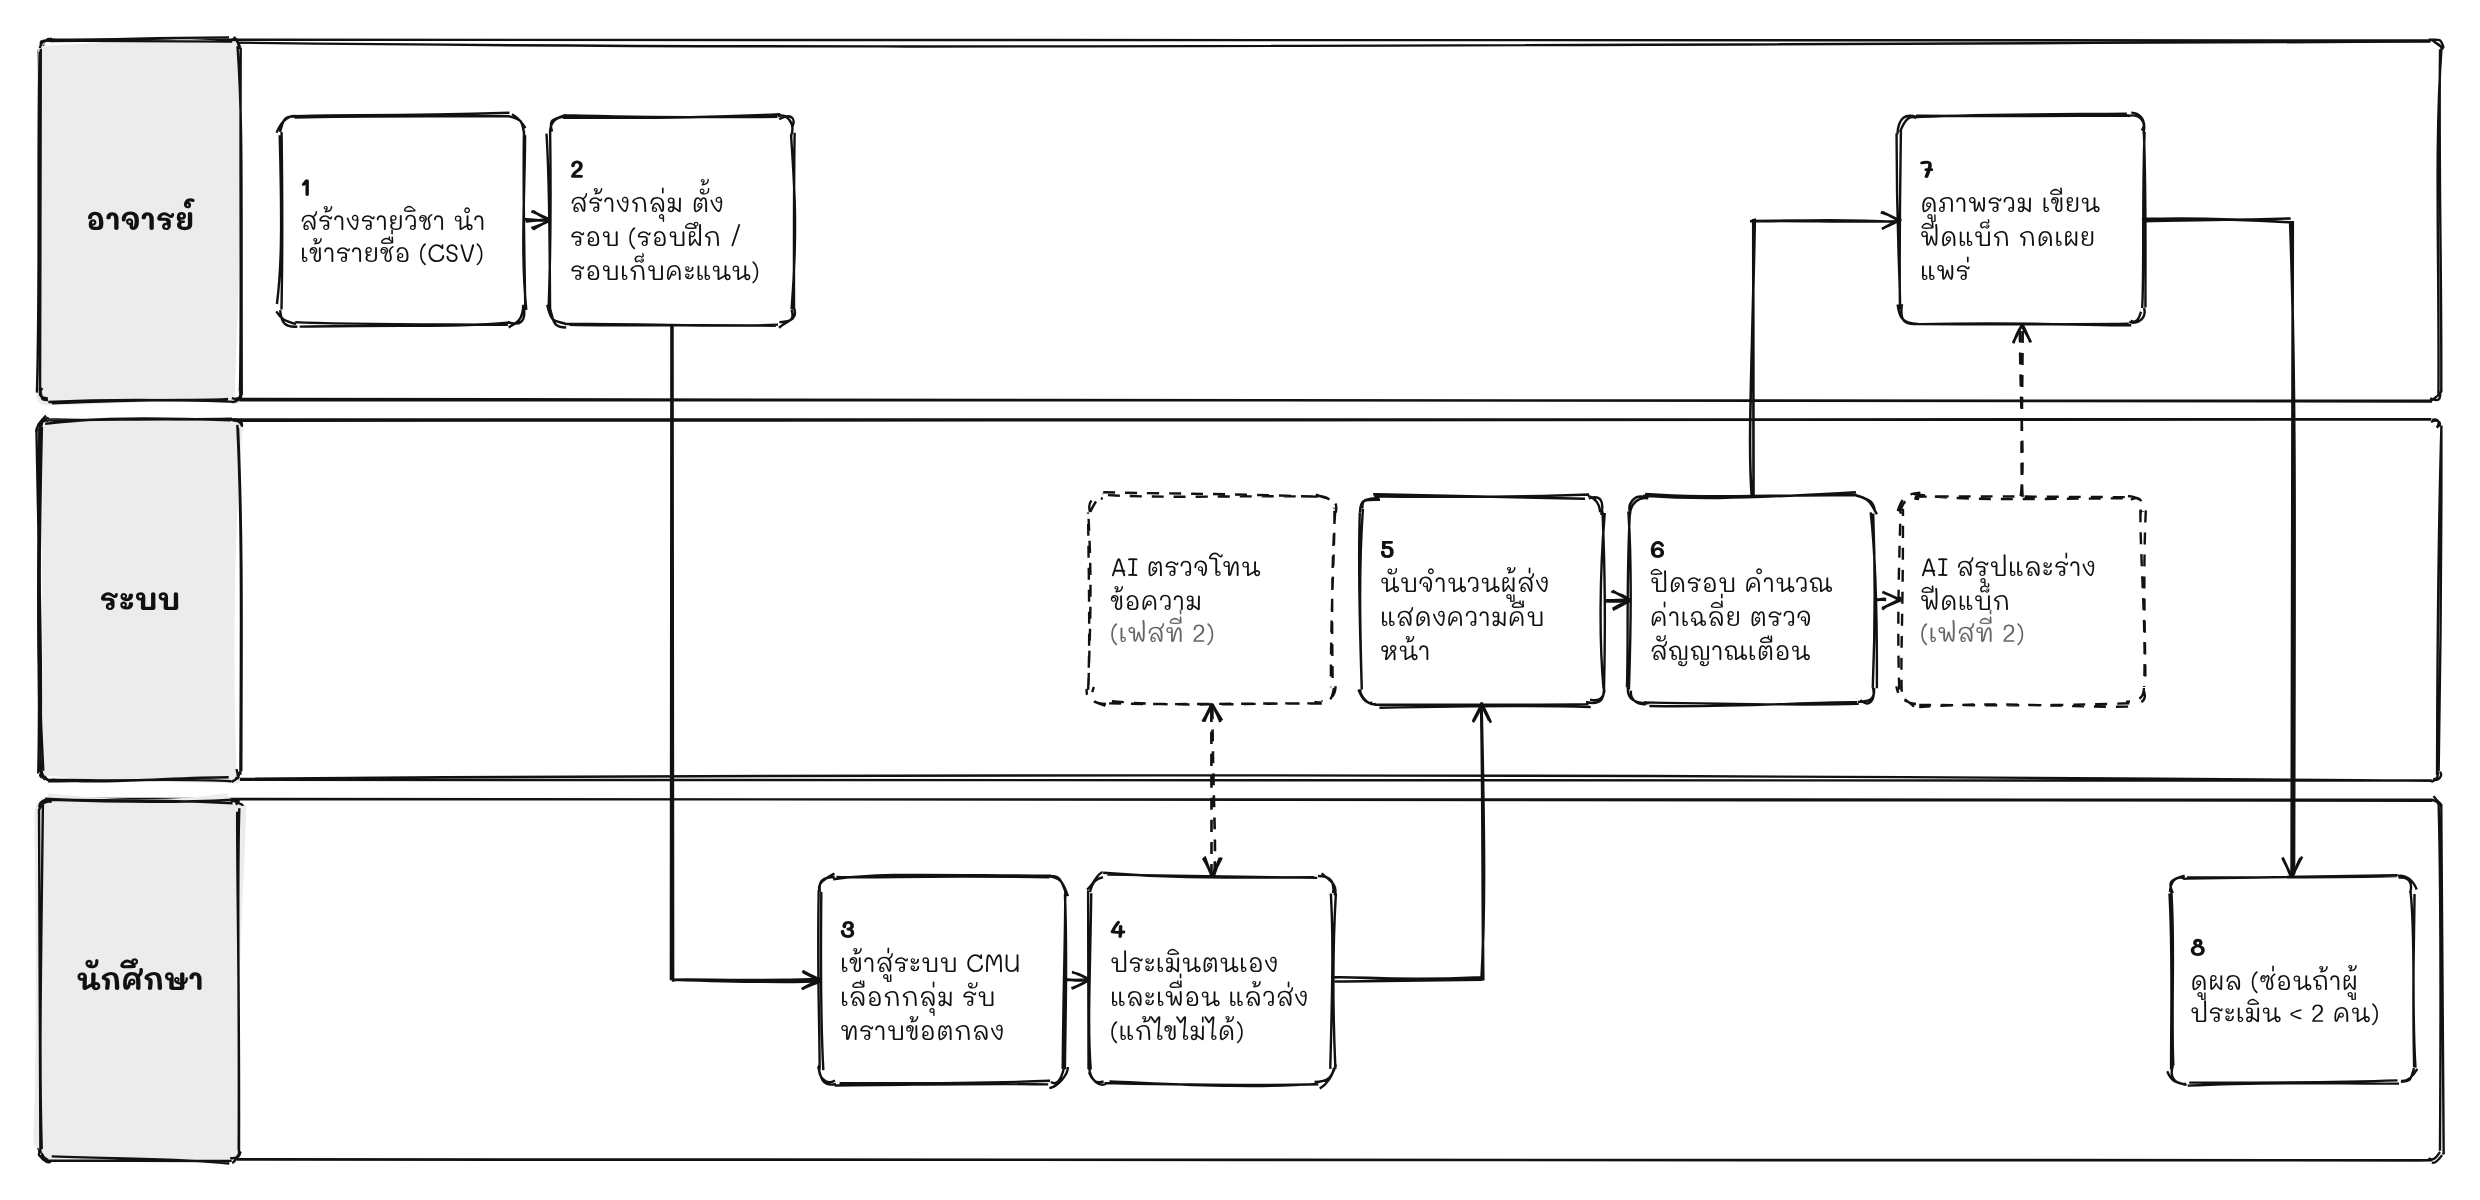
\includegraphics[width=\textwidth]{figures/ch3/fig3-1-swimlane.png}}{\fbox{\parbox{0.8\textwidth}{\centering\vspace{2cm}[วางไฟล์ figures/ch3/fig3-1-swimlane.png]\vspace{2cm}}}}
\caption{ขั้นตอนการทำงานของหนึ่งรอบประเมินแบบ swimlane}\label{fig:ch3-1}
\end{figure}

\subsection{การปกปิดตัวตนและสิทธิ์การมองเห็นข้อมูล}\label{sec:3.5.3}

ระบบไม่เปิดเผยตัวตนของผู้ประเมินต่อเพื่อน เพื่อให้นักศึกษากล้าให้ข้อเสนอแนะอย่างจริงใจ และให้นักศึกษาเห็นเฉพาะข้อมูลของตนเอง เพื่อลดการเปรียบเทียบและแข่งขันกันระหว่างเพื่อน สิทธิ์การมองเห็นข้อมูลแสดงในตารางที่~\ref{tab:ch3-8}

\begin{xltabular}{\textwidth}{|P{0.2\textwidth}|Y|P{0.12\textwidth}|Y|}
\caption{สิทธิ์การมองเห็นข้อมูลของผู้ใช้แต่ละบทบาท}\label{tab:ch3-8}\\
\hline \textbf{ข้อมูล} & \textbf{นักศึกษาเจ้าของข้อมูล} & \textbf{นักศึกษาคนอื่น} & \textbf{อาจารย์} \\ \hline
\endfirsthead
\multicolumn{4}{r}{\small (ต่อ)}\\ \hline \textbf{ข้อมูล} & \textbf{นักศึกษาเจ้าของข้อมูล} & \textbf{นักศึกษาคนอื่น} & \textbf{อาจารย์} \\ \hline
\endhead
คะแนนเฉลี่ยรายด้านที่เพื่อนประเมิน & เห็น เมื่อมีผู้ประเมินอย่างน้อย 2 คนและอาจารย์เผยแพร่แล้ว & ไม่เห็น & เห็น \\ \hline
คะแนนรายคนและชื่อผู้ประเมิน & ไม่เห็น & ไม่เห็น & เห็น เพื่อใช้ติดตามและกลั่นกรอง \\ \hline
ความเห็นปลายเปิด & เห็นหลังอาจารย์เผยแพร่ ในรูปแบบที่อาจารย์เลือก & ไม่เห็น & เห็นทั้งหมด \\ \hline
คะแนนที่ประเมินตนเอง & เห็น & ไม่เห็น & เห็น \\ \hline
สัญญาณเตือนและสถานะการส่ง & ไม่เห็น & ไม่เห็น & เห็น \\ \hline
\end{xltabular}

เงื่อนไขผู้ประเมินขั้นต่ำ 2 คนป้องกันไม่ให้นักศึกษาเดาได้ว่าใครเป็นผู้ประเมินในกรณีที่กลุ่มมีสมาชิกน้อย การบังคับสิทธิ์ทั้งหมดทำที่ฝั่ง API ไม่ใช่เพียงการซ่อนบนหน้าจอ ข้อมูลที่ผู้ใช้ไม่มีสิทธิ์จึงไม่ถูกส่งออกจากเซิร์ฟเวอร์เลย

\subsection{สัญญาณเตือน การเผยแพร่ผล และการสื่อสาร}\label{sec:3.5.4}

ในระยะที่ 1 ระบบสร้างสัญญาณเตือนจากรูปแบบคะแนนตามเงื่อนไขที่กำหนดไว้ (rule-based) เช่น คะแนนเฉลี่ยที่เพื่อนให้ต่ำในด้านใดด้านหนึ่ง คะแนนที่ประเมินตนเองต่างจากที่เพื่อนประเมินมาก หรือยังไม่ส่งแบบประเมิน เพื่อชี้ให้อาจารย์รู้ว่าควรดูแลทีมใดก่อน ฐานข้อมูลเก็บแหล่งที่มาของสัญญาณไว้ด้วย จึงรองรับสัญญาณจากปัญญาประดิษฐ์ (AI) ในระยะที่ 2 ได้โดยไม่ต้องเปลี่ยนโครงสร้าง

ผลการประเมินจะไม่ถึงนักศึกษาโดยอัตโนมัติ อาจารย์เป็นผู้ตรวจทานและกดเผยแพร่ทุกครั้ง โดยเลือกได้ว่าจะแสดงความเห็นของเพื่อนตามจริง หรือแสดงเป็นข้อสรุปที่อาจารย์เขียน การสื่อสารเป็นแบบทางเดียว นักศึกษาตอบกลับความเห็นของเพื่อนในระบบไม่ได้ เพราะการโต้ตอบอาจทำให้สืบทราบตัวตนผู้ประเมินได้ หากนักศึกษามีข้อสงสัยให้สื่อสารผ่านอาจารย์ นอกจากนี้ระบบออกแบบให้ใช้ร่วมกับกิจกรรมในชั้นเรียน เช่น อาจารย์อาจจัดเวลาประมาณ 1 ชั่วโมงให้นักศึกษาพูดคุยเรื่องข้อเสนอแนะกันแบบพบหน้า เพื่อไม่ให้การให้ข้อเสนอแนะผ่านระบบออนไลน์เพียงอย่างเดียวดูห่างเหิน

\section{การออกแบบส่วน AI (ระยะที่ 2)}\label{sec:3.6}

\subsection{ที่มาของการใช้ปัญญาประดิษฐ์}\label{sec:3.6.1}

การเรียนรู้ในปัจจุบันต้องปรับตัวกับการที่ทั้งผู้เรียนและผู้สอนใช้เครื่องมือปัญญาประดิษฐ์ (AI) มากขึ้น ระบบจึงนำปัญญาประดิษฐ์ มาใช้เฉพาะงานที่ปัญญาประดิษฐ์ (AI) ทำได้ดีและลดภาระคนได้จริง คือการอ่านและสรุปข้อความจำนวนมาก และการช่วยเกลาภาษา โดยไม่ให้ปัญญาประดิษฐ์ (AI) ตัดสินใจแทนคน ส่วนปัญญาประดิษฐ์ (AI) จัดอยู่ในการพัฒนาระยะที่ 2 โดยระบบใช้โมเดลภาษา Qwen ผ่าน API และแบ่งเป็น 2 ส่วน ดังรูปที่~\ref{fig:ch3-2}

\begin{figure}[htbp]
\centering
\IfFileExists{figures/ch3/fig3-2-ai.png}{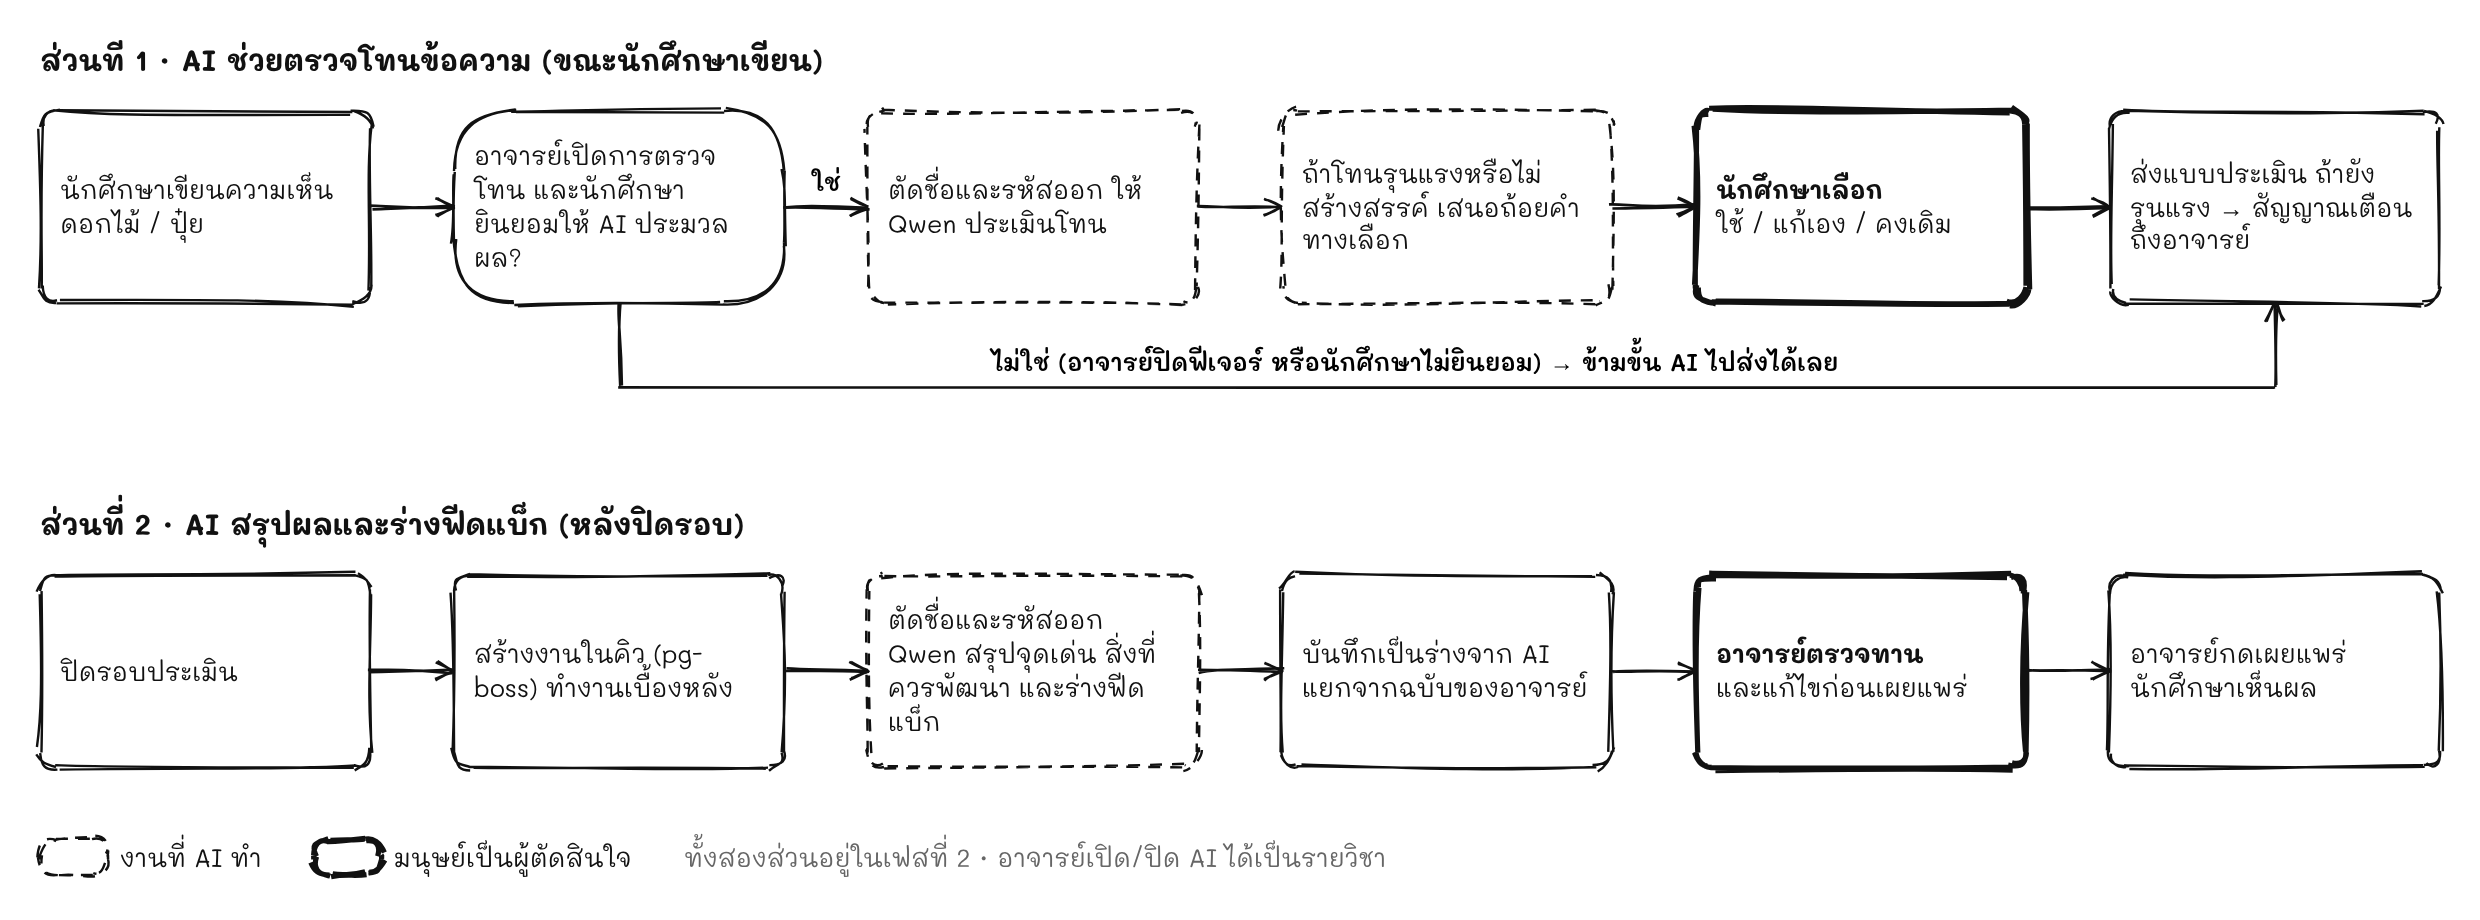
\includegraphics[width=\textwidth]{figures/ch3/fig3-2-ai.png}}{\fbox{\parbox{0.8\textwidth}{\centering\vspace{2cm}[วางไฟล์ figures/ch3/fig3-2-ai.png]\vspace{2cm}}}}
\caption{การทำงานของส่วน AI ทั้ง 2 ส่วน}\label{fig:ch3-2}
\end{figure}

\subsection{ปัญญาประดิษฐ์ช่วยตรวจโทนข้อความ}\label{sec:3.6.2}

อาจารย์เลือกเปิดหรือปิดฟีเจอร์นี้ได้เป็นรายวิชา เมื่อเปิดใช้งาน ขณะนักศึกษาเขียนความเห็นปลายเปิด ระบบส่งข้อความให้โมเดลประเมินโทน หากข้อความมีลักษณะรุนแรง ตำหนิตัวบุคคล หรือไม่สร้างสรรค์ ระบบจะแสดงคำเตือนพร้อมเสนอถ้อยคำทางเลือกที่สื่อประเด็นเดิมอย่างสร้างสรรค์ นักศึกษาเป็นผู้ตัดสินใจเองว่าจะใช้ถ้อยคำที่เสนอ แก้ไขเอง หรือคงข้อความเดิม ระบบไม่เปลี่ยนข้อความให้โดยอัตโนมัติ หากข้อความที่ส่งแล้วยังมีโทนรุนแรง ระบบจะบันทึกเป็นสัญญาณเตือนให้อาจารย์เห็น หากอาจารย์ปิดฟีเจอร์นี้ นักศึกษาจะเขียนและส่งความเห็นได้ตามปกติโดยไม่ผ่านการตรวจโทน

\subsection{ปัญญาประดิษฐ์สรุปผลและร่างข้อเสนอแนะ}\label{sec:3.6.3}

เมื่อปิดรอบประเมิน ระบบรวบรวมความเห็นที่นักศึกษาแต่ละคนได้รับ แล้วส่งให้โมเดลสรุปเป็นจุดเด่นและสิ่งที่ควรพัฒนา พร้อมร่างข้อเสนอแนะถึงนักศึกษาคนนั้น ร่างจากปัญญาประดิษฐ์ (AI) ถูกเก็บแยกจากฉบับที่อาจารย์แก้ไข และอาจารย์ต้องตรวจทานก่อนเผยแพร่ทุกครั้ง การประมวลผลทำผ่านคิวงานเบื้องหลัง ผู้ใช้จึงไม่ต้องรอระหว่างที่โมเดลทำงาน

\subsection{หลักการกำกับการใช้ปัญญาประดิษฐ์ (AI)}\label{sec:3.6.4}

\begin{itemize}
  \item มนุษย์ตัดสินใจขั้นสุดท้ายเสมอ (human-in-the-loop): AI ทำหน้าที่เสนอ ส่วนนักศึกษาและอาจารย์เป็นผู้เลือก
  \item เปิดหรือปิดได้: อาจารย์เปิดหรือปิดฟีเจอร์ปัญญาประดิษฐ์ (AI) ได้เป็นรายวิชา และข้อความของนักศึกษาจะถูกส่งให้ปัญญาประดิษฐ์ (AI) เฉพาะเมื่อนักศึกษายินยอมในส่วนทางเลือก (หัวข้อ~\ref{sec:3.9.2})
  \item ลดข้อมูลที่ส่งออก: ส่งเฉพาะข้อความที่ต้องประมวลผล โดยไม่ส่งชื่อหรือรหัสนักศึกษาไปยังผู้ให้บริการโมเดล
  \item ยอมรับข้อจำกัด: โมเดลอาจตีความภาษาไทยผิด โดยเฉพาะถ้อยคำประชดประชันซึ่งจัดเป็นงานในระยะที่ 3 นี่คือเหตุผลที่ระบบไม่ให้ปัญญาประดิษฐ์ (AI) ตัดสินใจเอง
\end{itemize}

\section{สถาปัตยกรรมระบบและฐานข้อมูล}\label{sec:3.7}

\subsection{ภาพรวมสถาปัตยกรรม}\label{sec:3.7.1}

ระบบเป็นเว็บแอปพลิเคชันที่แยกส่วนหน้า (frontend) และส่วนหลัง (backend) ออกจากกัน และสื่อสารกันผ่าน REST API ด้วยข้อมูลรูปแบบ JSON องค์ประกอบหลักแสดงในรูปที่~\ref{fig:ch3-3} ดังนี้

\begin{itemize}
  \item ส่วนหน้า: React 19, Vite และ TypeScript จัดหน้าตาด้วย Tailwind CSS จัดการข้อมูลจากเซิร์ฟเวอร์ด้วย TanStack Query และจัดการสถานะภายในหน้าเว็บด้วย Zustand
  \item เว็บเซิร์ฟเวอร์: nginx ให้บริการไฟล์ของส่วนหน้า ทำหน้าที่ reverse proxy ไปยัง API และจัดการ HTTPS
  \item ส่วนหลัง: Node.js และ Express 5 เข้าถึงฐานข้อมูลผ่าน Drizzle ORM และกำหนดสัญญาการเชื่อมต่อ API ด้วย OpenAPI
  \item ฐานข้อมูล: PostgreSQL เก็บข้อมูลของระบบ เซสชันผู้ใช้ และคิวงานเบื้องหลัง (pg-boss)
  \item Worker และบริการ AI (เฟสที่ 2): worker ดึงงานจากคิวไปเรียกโมเดล Qwen ผ่าน API แล้วบันทึกผลกลับลงฐานข้อมูล
\end{itemize}

คณะผู้จัดทำเลือกใช้ PostgreSQL เป็นทั้งที่เก็บเซสชันและคิวงาน แทนการเพิ่ม Redis และ BullMQ ซึ่งเป็นอีกทางเลือกหนึ่ง เพื่อลดจำนวนบริการที่ต้องดูแลและใช้ทรัพยากรน้อยลง ทางเลือกนี้เหมาะกับข้อจำกัดของเซิร์ฟเวอร์ขนาด 2 vCPU หน่วยความจำ 4 GB ตามงบประมาณของโครงงาน และปริมาณงานของระบบในระดับรายวิชาซึ่งไม่ได้ต้องการความเร็วที่สูงมาก

\begin{figure}[htbp]
\centering
\IfFileExists{figures/ch3/fig3-3-architecture.png}{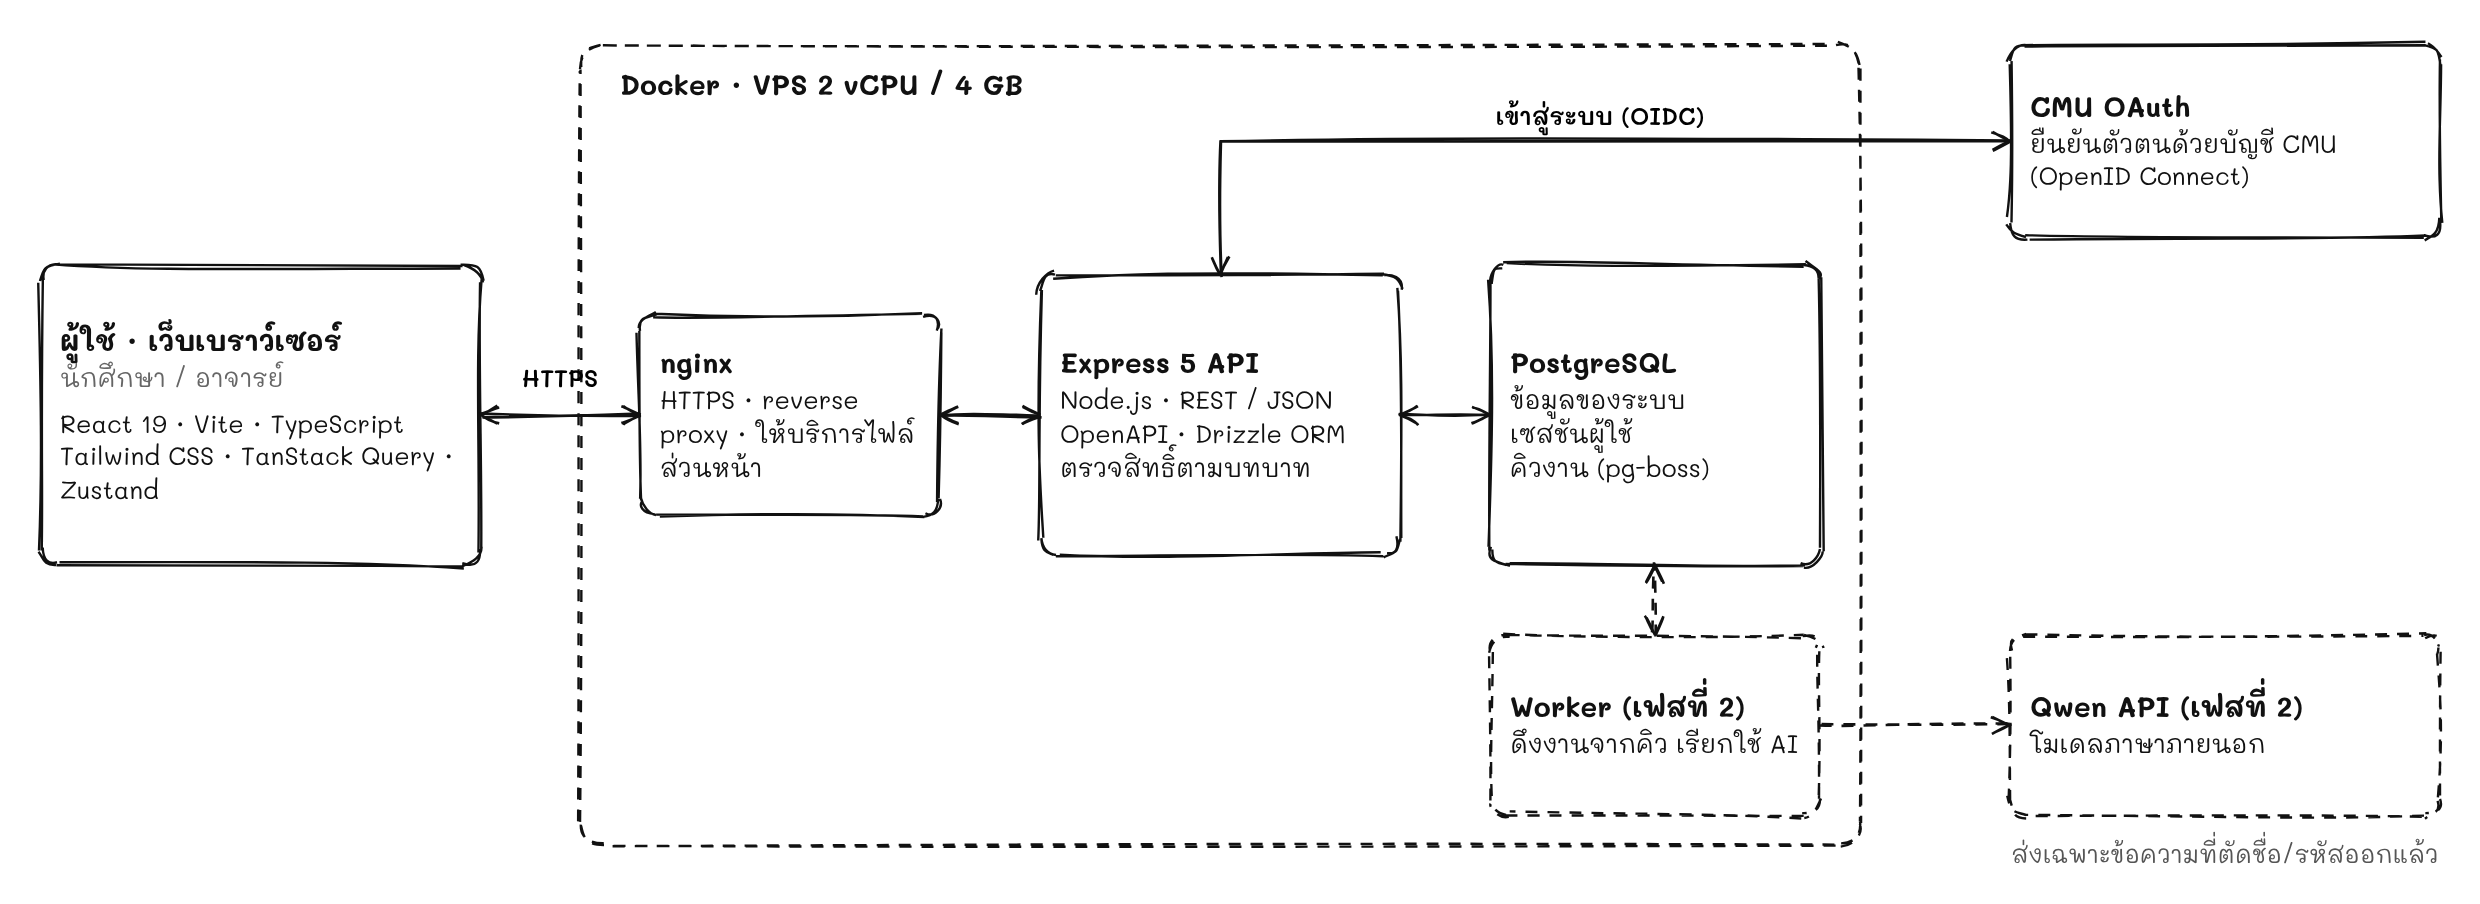
\includegraphics[width=\textwidth]{figures/ch3/fig3-3-architecture.png}}{\fbox{\parbox{0.8\textwidth}{\centering\vspace{2cm}[วางไฟล์ figures/ch3/fig3-3-architecture.png]\vspace{2cm}}}}
\caption{สถาปัตยกรรมของระบบ}\label{fig:ch3-3}
\end{figure}

\subsection{การยืนยันตัวตน}\label{sec:3.7.2}

ผู้ใช้เข้าสู่ระบบด้วยบัญชี CMU ผ่าน CMU OAuth ตามมาตรฐาน OpenID Connect~\cite{sakimura2014oidc} ระบบจึงไม่ต้องเก็บรหัสผ่านของผู้ใช้เอง หลังยืนยันตัวตน เซิร์ฟเวอร์สร้างเซสชันที่เก็บในฐานข้อมูล และส่งคุกกี้เซสชันแบบ HttpOnly และ Secure ให้เบราว์เซอร์ บทบาทของผู้ใช้ในแต่ละรายวิชา (นักศึกษาหรืออาจารย์) ถูกตรวจสอบทุกครั้งที่เรียก API

\subsection{การออกแบบฐานข้อมูล}\label{sec:3.7.3}

ฐานข้อมูลเป็นแบบเชิงสัมพันธ์ ประกอบด้วยตารางที่ระยะที่ 1 ใช้ และตารางที่เตรียมไว้สำหรับระยะถัดไป ได้แก่ ตารางสัญญาณเตือน (flags) และตารางสรุปผล (ai\_feedback\_summaries) สำหรับปัญญาประดิษฐ์ (AI) และตารางบันทึกการซิงก์ข้อมูล (external\_sync\_logs) สำหรับการเชื่อมต่อระบบภายนอก ความสัมพันธ์ของข้อมูลแสดงในรูปที่~\ref{fig:ch3-4} โดยมีการตัดสินใจออกแบบที่สำคัญดังนี้

\begin{itemize}
  \item ตารางคะแนน (ratings) ให้ช่องผู้ถูกประเมินเป็นค่าว่างได้ เพื่อรองรับคำถามระดับทีมที่ไม่ได้ประเมินบุคคลใดบุคคลหนึ่ง
  \item ตารางสรุปผล (ai\_feedback\_summaries) เก็บทั้งร่างจากปัญญาประดิษฐ์ (AI) และฉบับสุดท้ายที่อาจารย์แก้ไข เพื่อแยกให้เห็นว่าส่วนใดมาจากปัญญาประดิษฐ์ (AI) และส่วนใดผ่านการตรวจทานแล้ว
  \item ตารางความยินยอม (consents) เก็บเวอร์ชันของนโยบายที่ผู้ใช้ยินยอม เพื่อขอความยินยอมใหม่ได้เมื่อนโยบายเปลี่ยน
  \item ตารางสัญญาณเตือน (flags) มีช่องระบุแหล่งที่มาของสัญญาณ เพื่อรองรับทั้งสัญญาณจากเงื่อนไขคะแนนและจากปัญญาประดิษฐ์ (AI)
  \item ตารางรายวิชาและผู้ใช้มีช่องเก็บรหัสอ้างอิงจากระบบภายนอก เพื่อเตรียมเชื่อมต่อ Mango Canvas ในระยะที่ 3 โดยมีตารางบันทึกการซิงก์ข้อมูล (external\_sync\_logs) เก็บผลการนำเข้ารายชื่อและส่งออกคะแนนของแต่ละรายวิชา
  \item ตารางระดับเกณฑ์การให้คะแนน (rubric\_levels) เก็บคำอธิบายพฤติกรรมของแต่ละคะแนนในคำถามแบบให้คะแนน เพื่อให้ผู้ประเมินใช้เกณฑ์เดียวกัน
\end{itemize}

\begin{sidewaysfigure}
\centering
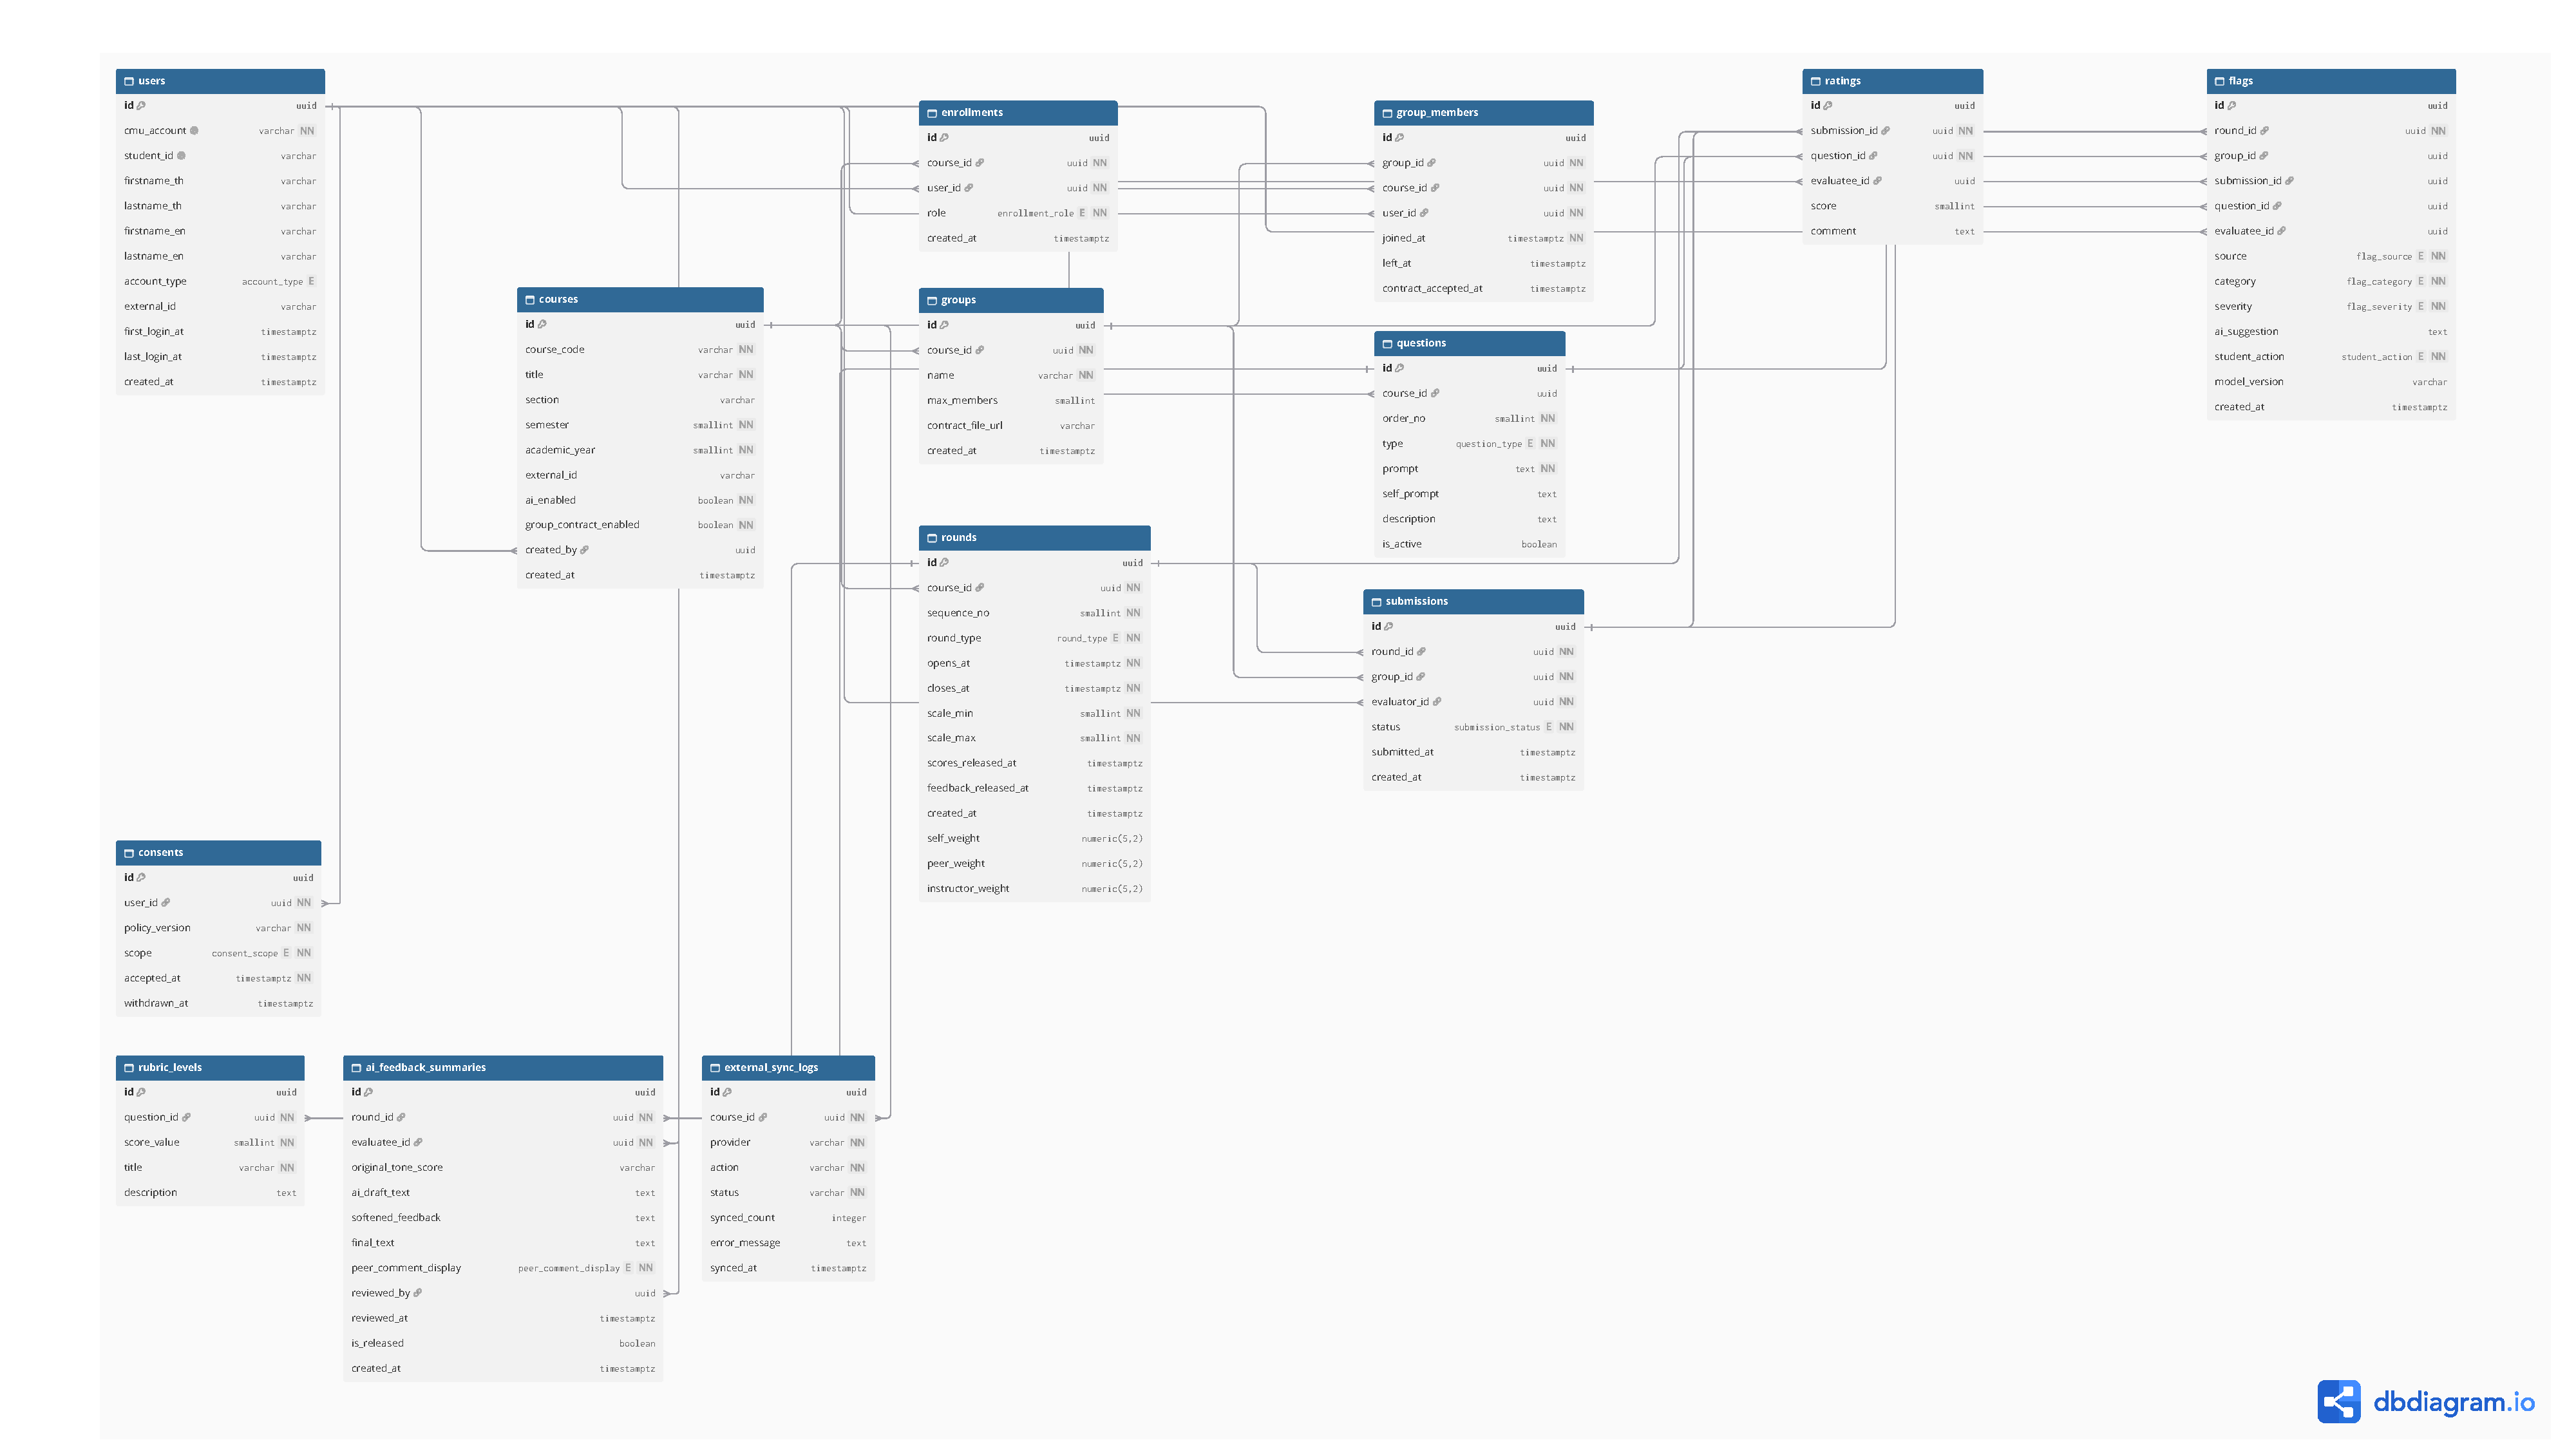
\includegraphics[width=\linewidth]{figures/ch3/fig3-4-er.pdf}
\caption{แผนภาพความสัมพันธ์ของข้อมูล (ER diagram)}\label{fig:ch3-4}
\end{sidewaysfigure}

\subsection{การติดตั้งและการทดสอบ}\label{sec:3.7.4}

ทุกบริการถูกบรรจุเป็น Docker container และติดตั้งบนเซิร์ฟเวอร์เสมือน (VPS) ขนาด 2 vCPU หน่วยความจำ 4 GB การทดสอบใช้ Vitest สำหรับ unit test และ integration test และใช้ Cypress สำหรับ end-to-end test ส่วนการสำรองข้อมูล การตรวจสอบสถานะระบบ และการส่งอีเมล ใช้บริการแบบไม่มีค่าใช้จ่าย

\section{การออกแบบส่วนต่อประสานผู้ใช้}\label{sec:3.8}

\subsection{หลักการออกแบบ}\label{sec:3.8.1}

\begin{itemize}
  \item นำทางตามงาน: แถบเมนูด้านข้างจัดตามงานที่ผู้ใช้ต้องทำ พร้อมตัวเลขแจ้งจำนวนงานค้าง
  \item แสดงสถานะด้วยป้ายสถานะ (status pill) เช่น เปิดรับ ปิดแล้ว และรอเผยแพร่
  \item แบบประเมินแสดงทีละคำถามต่อหน้าจอ เพื่อลดภาระการอ่านและใช้งานบนมือถือได้สะดวก
  \item ออกแบบตามแนวทาง WCAG 2.2~\cite{w3c2023wcag} เช่น ความต่างของสีตัวอักษรกับพื้นหลังที่เพียงพอ การใช้งานด้วยแป้นพิมพ์ และการติดป้ายกำกับช่องกรอกทุกช่อง
\end{itemize}

หน้าจอทั้งหมดออกแบบเป็นต้นแบบความละเอียดต่ำ (low-fidelity wireframe) แบบขาวดำก่อนพัฒนาจริง และใช้ต้นแบบนี้สื่อสารทั้งภายในทีมและกับอาจารย์ผู้ใช้ เพื่อรับความคิดเห็นก่อนลงมือพัฒนา

\subsection{หน้าจอฝั่งนักศึกษา}\label{sec:3.8.2}

ผู้ใช้เข้าสู่ระบบด้วยบัญชี CMU ผ่าน CMU OAuth โดยไม่ต้องสร้างรหัสผ่านใหม่ ดังรูปที่~\ref{fig:ch3-5}

\begin{figure}[htbp]
\centering
\IfFileExists{figures/ch3/fig3-5-login.png}{
\includegraphics[width=\textwidth]{figures/ch3/fig3-5-login.png}}{\fbox{\parbox{0.8\textwidth}{\centering\vspace{2cm}[วางไฟล์ figures/ch3/fig3-5-login.png]\vspace{2cm}}}}
\caption{หน้าเข้าสู่ระบบ}\label{fig:ch3-5}
\end{figure}

ครั้งแรกที่เข้าใช้งาน นักศึกษาต้องอ่านข้อตกลงการใช้ข้อมูลส่วนบุคคล ซึ่งแบ่งจอเป็น 2 ส่วน ด้านซ้ายย้ำว่าความเห็นถึงเพื่อนจะไม่ระบุชื่อ ด้านขวาแสดงว่าเก็บข้อมูลอะไร ใครเห็น เก็บนานเท่าใด และสิทธิ์ของเจ้าของข้อมูล พร้อมตัวเลือกส่วนจำเป็นและส่วนทางเลือก ดังรูปที่~\ref{fig:ch3-6}

\begin{figure}[htbp]
\centering
\IfFileExists{figures/ch3/fig3-6-consent.png}{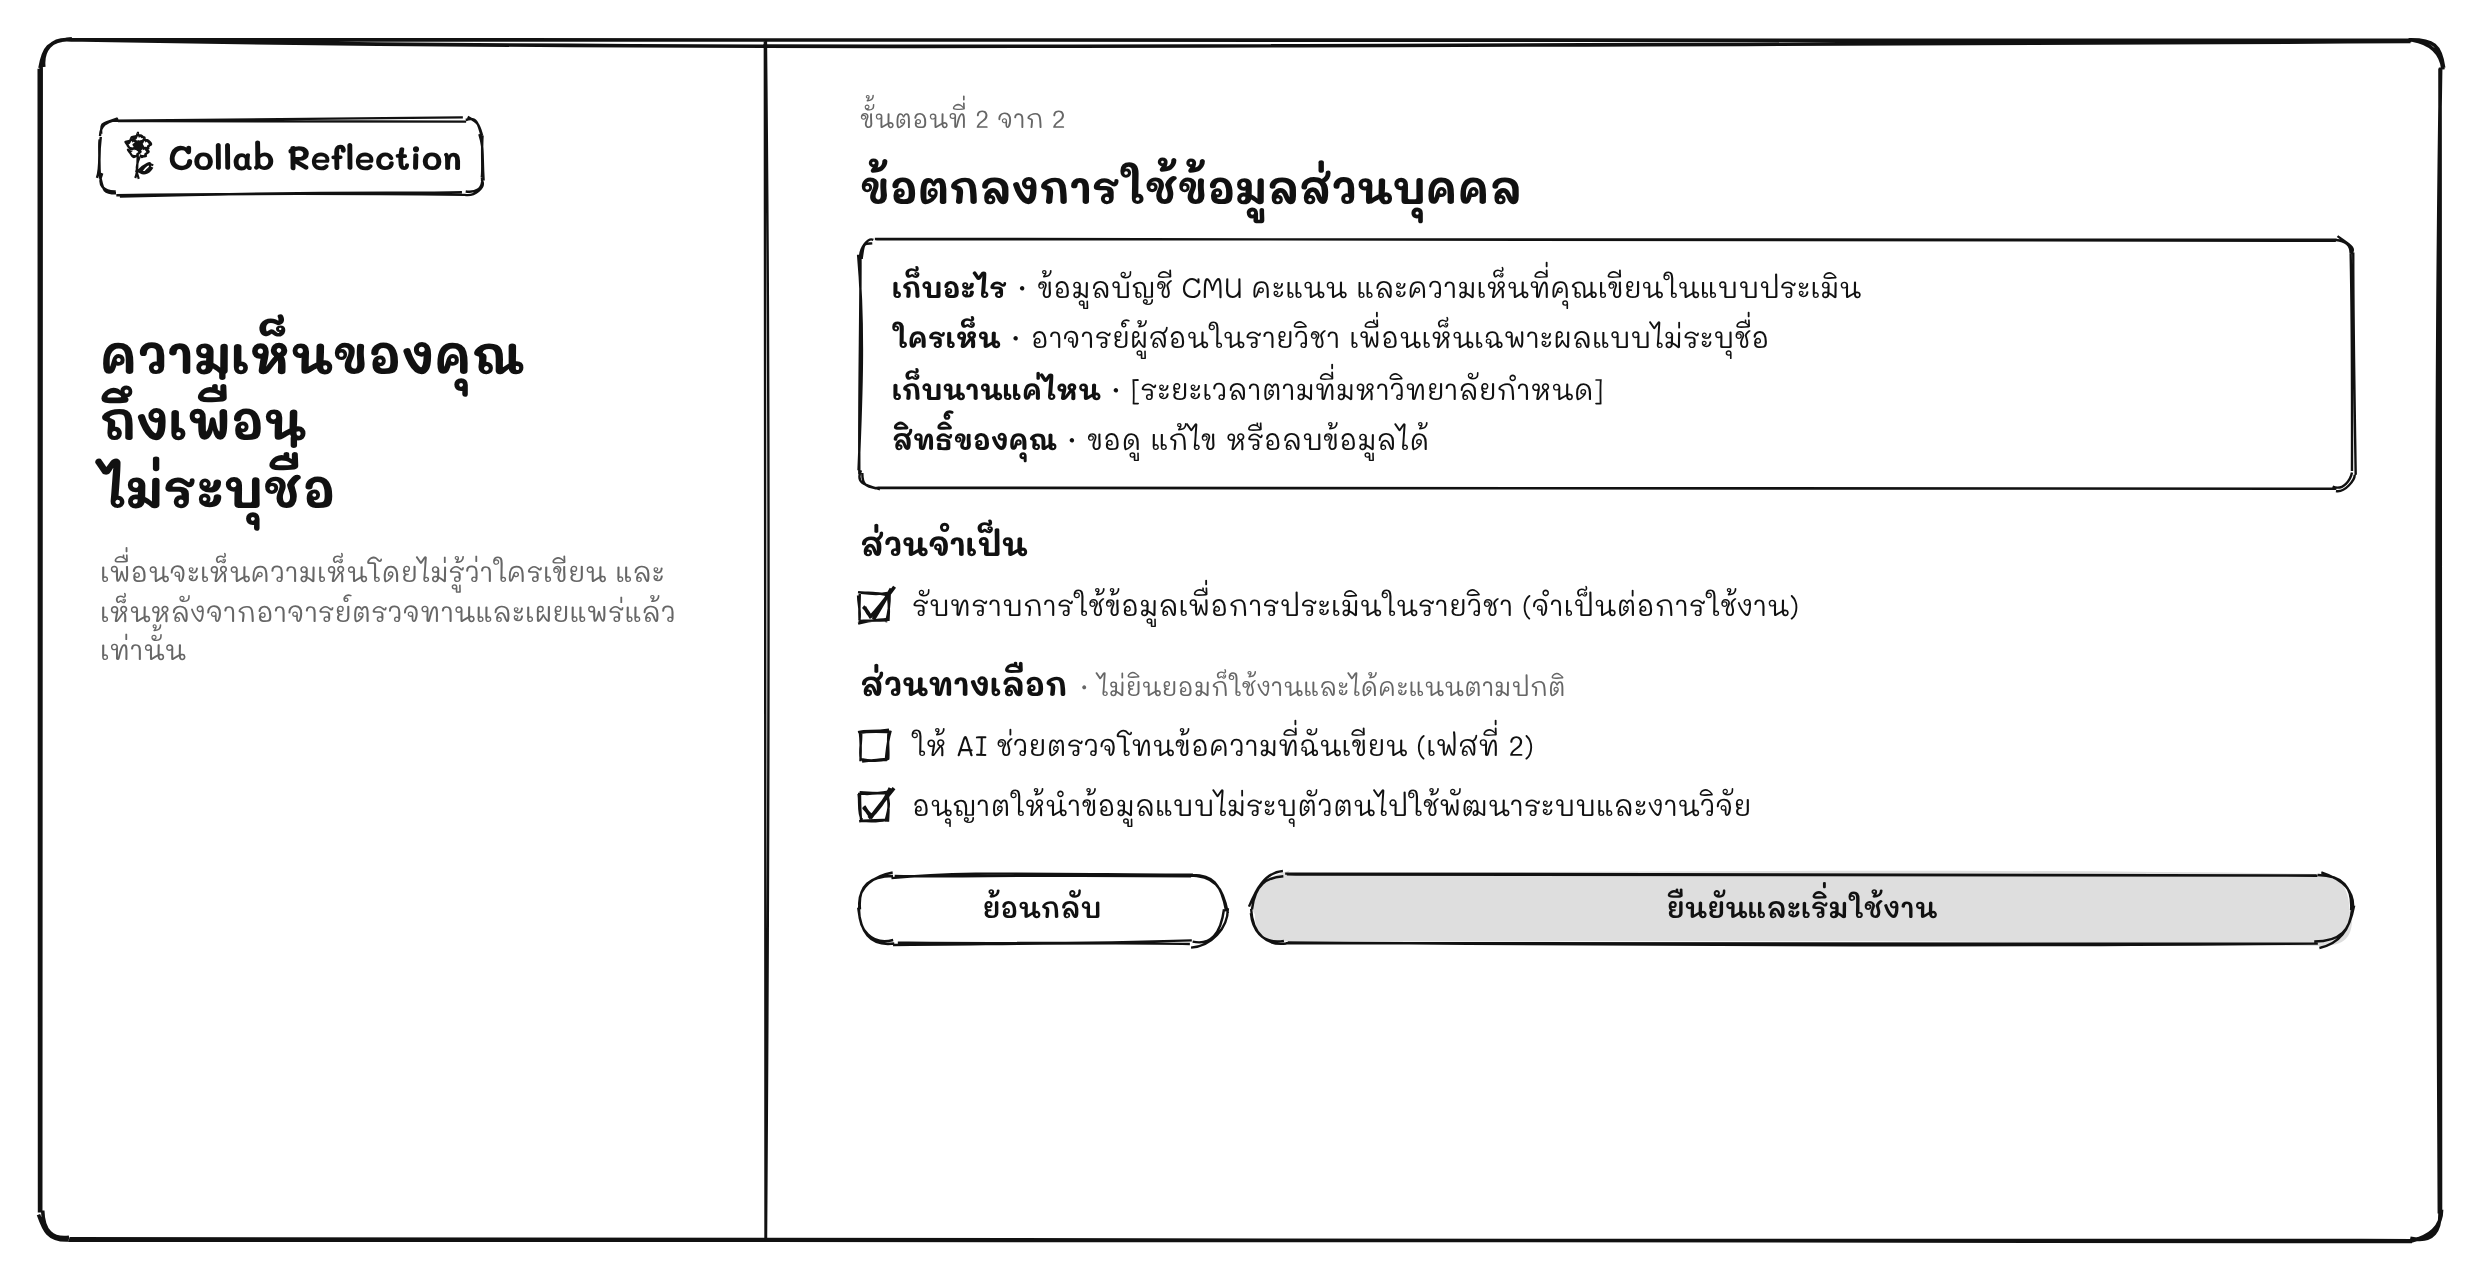
\includegraphics[width=\textwidth]{figures/ch3/fig3-6-consent.png}}{\fbox{\parbox{0.8\textwidth}{\centering\vspace{2cm}[วางไฟล์ figures/ch3/fig3-6-consent.png]\vspace{2cm}}}}
\caption{หน้าข้อตกลงการใช้ข้อมูลส่วนบุคคล}\label{fig:ch3-6}
\end{figure}

หน้ารายวิชาแสดงกลุ่มของนักศึกษา ข้อตกลงกลุ่ม และรายการรอบประเมิน โดยทุกรอบมีป้ายบอกว่าเป็นรอบฝึกหรือรอบเก็บคะแนน พร้อมสถานะของรอบ ดังรูปที่~\ref{fig:ch3-7}

\begin{figure}[htbp]
\centering
\IfFileExists{figures/ch3/fig3-7-student-course.png}{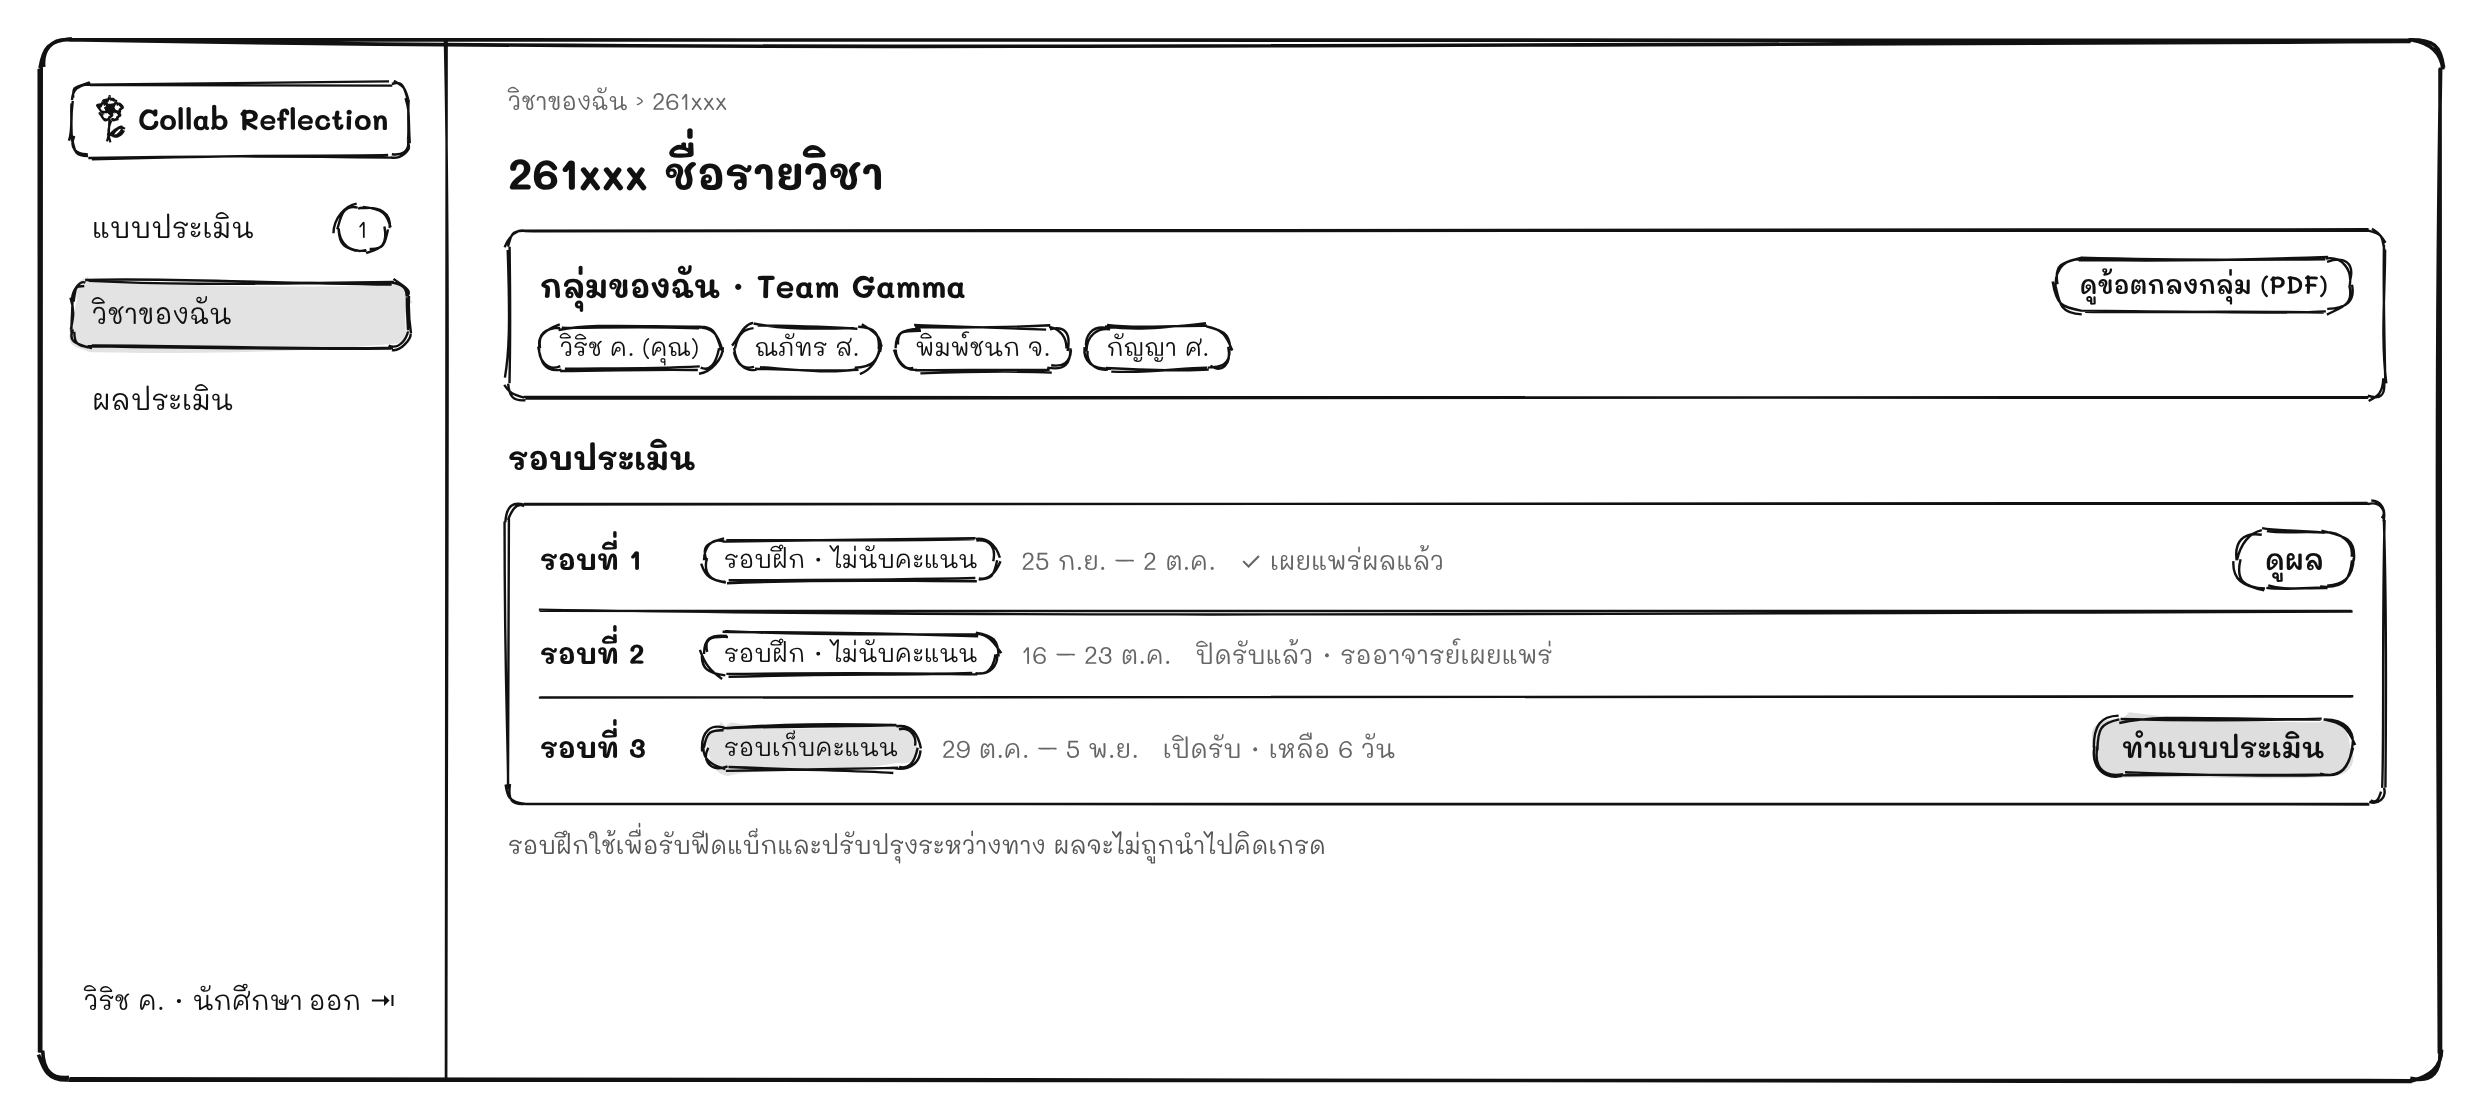
\includegraphics[width=\textwidth]{figures/ch3/fig3-7-student-course.png}}{\fbox{\parbox{0.8\textwidth}{\centering\vspace{2cm}[วางไฟล์ figures/ch3/fig3-7-student-course.png]\vspace{2cm}}}}
\caption{หน้ารายวิชาและรอบประเมินของนักศึกษา}\label{fig:ch3-7}
\end{figure}

แบบประเมินแสดงทีละด้านต่อหน้าจอ ด้านบนมีคำอธิบายพฤติกรรมของระดับ 1, 3 และ 5 ให้นักศึกษาให้คะแนนสมาชิกทุกคนรวมถึงตนเอง และด้านขวามีแถบแสดงขั้นตอนทั้ง 7 ขั้น ดังรูปที่~\ref{fig:ch3-8}

\begin{figure}[htbp]
\centering
\IfFileExists{figures/ch3/fig3-8-student-rating.png}{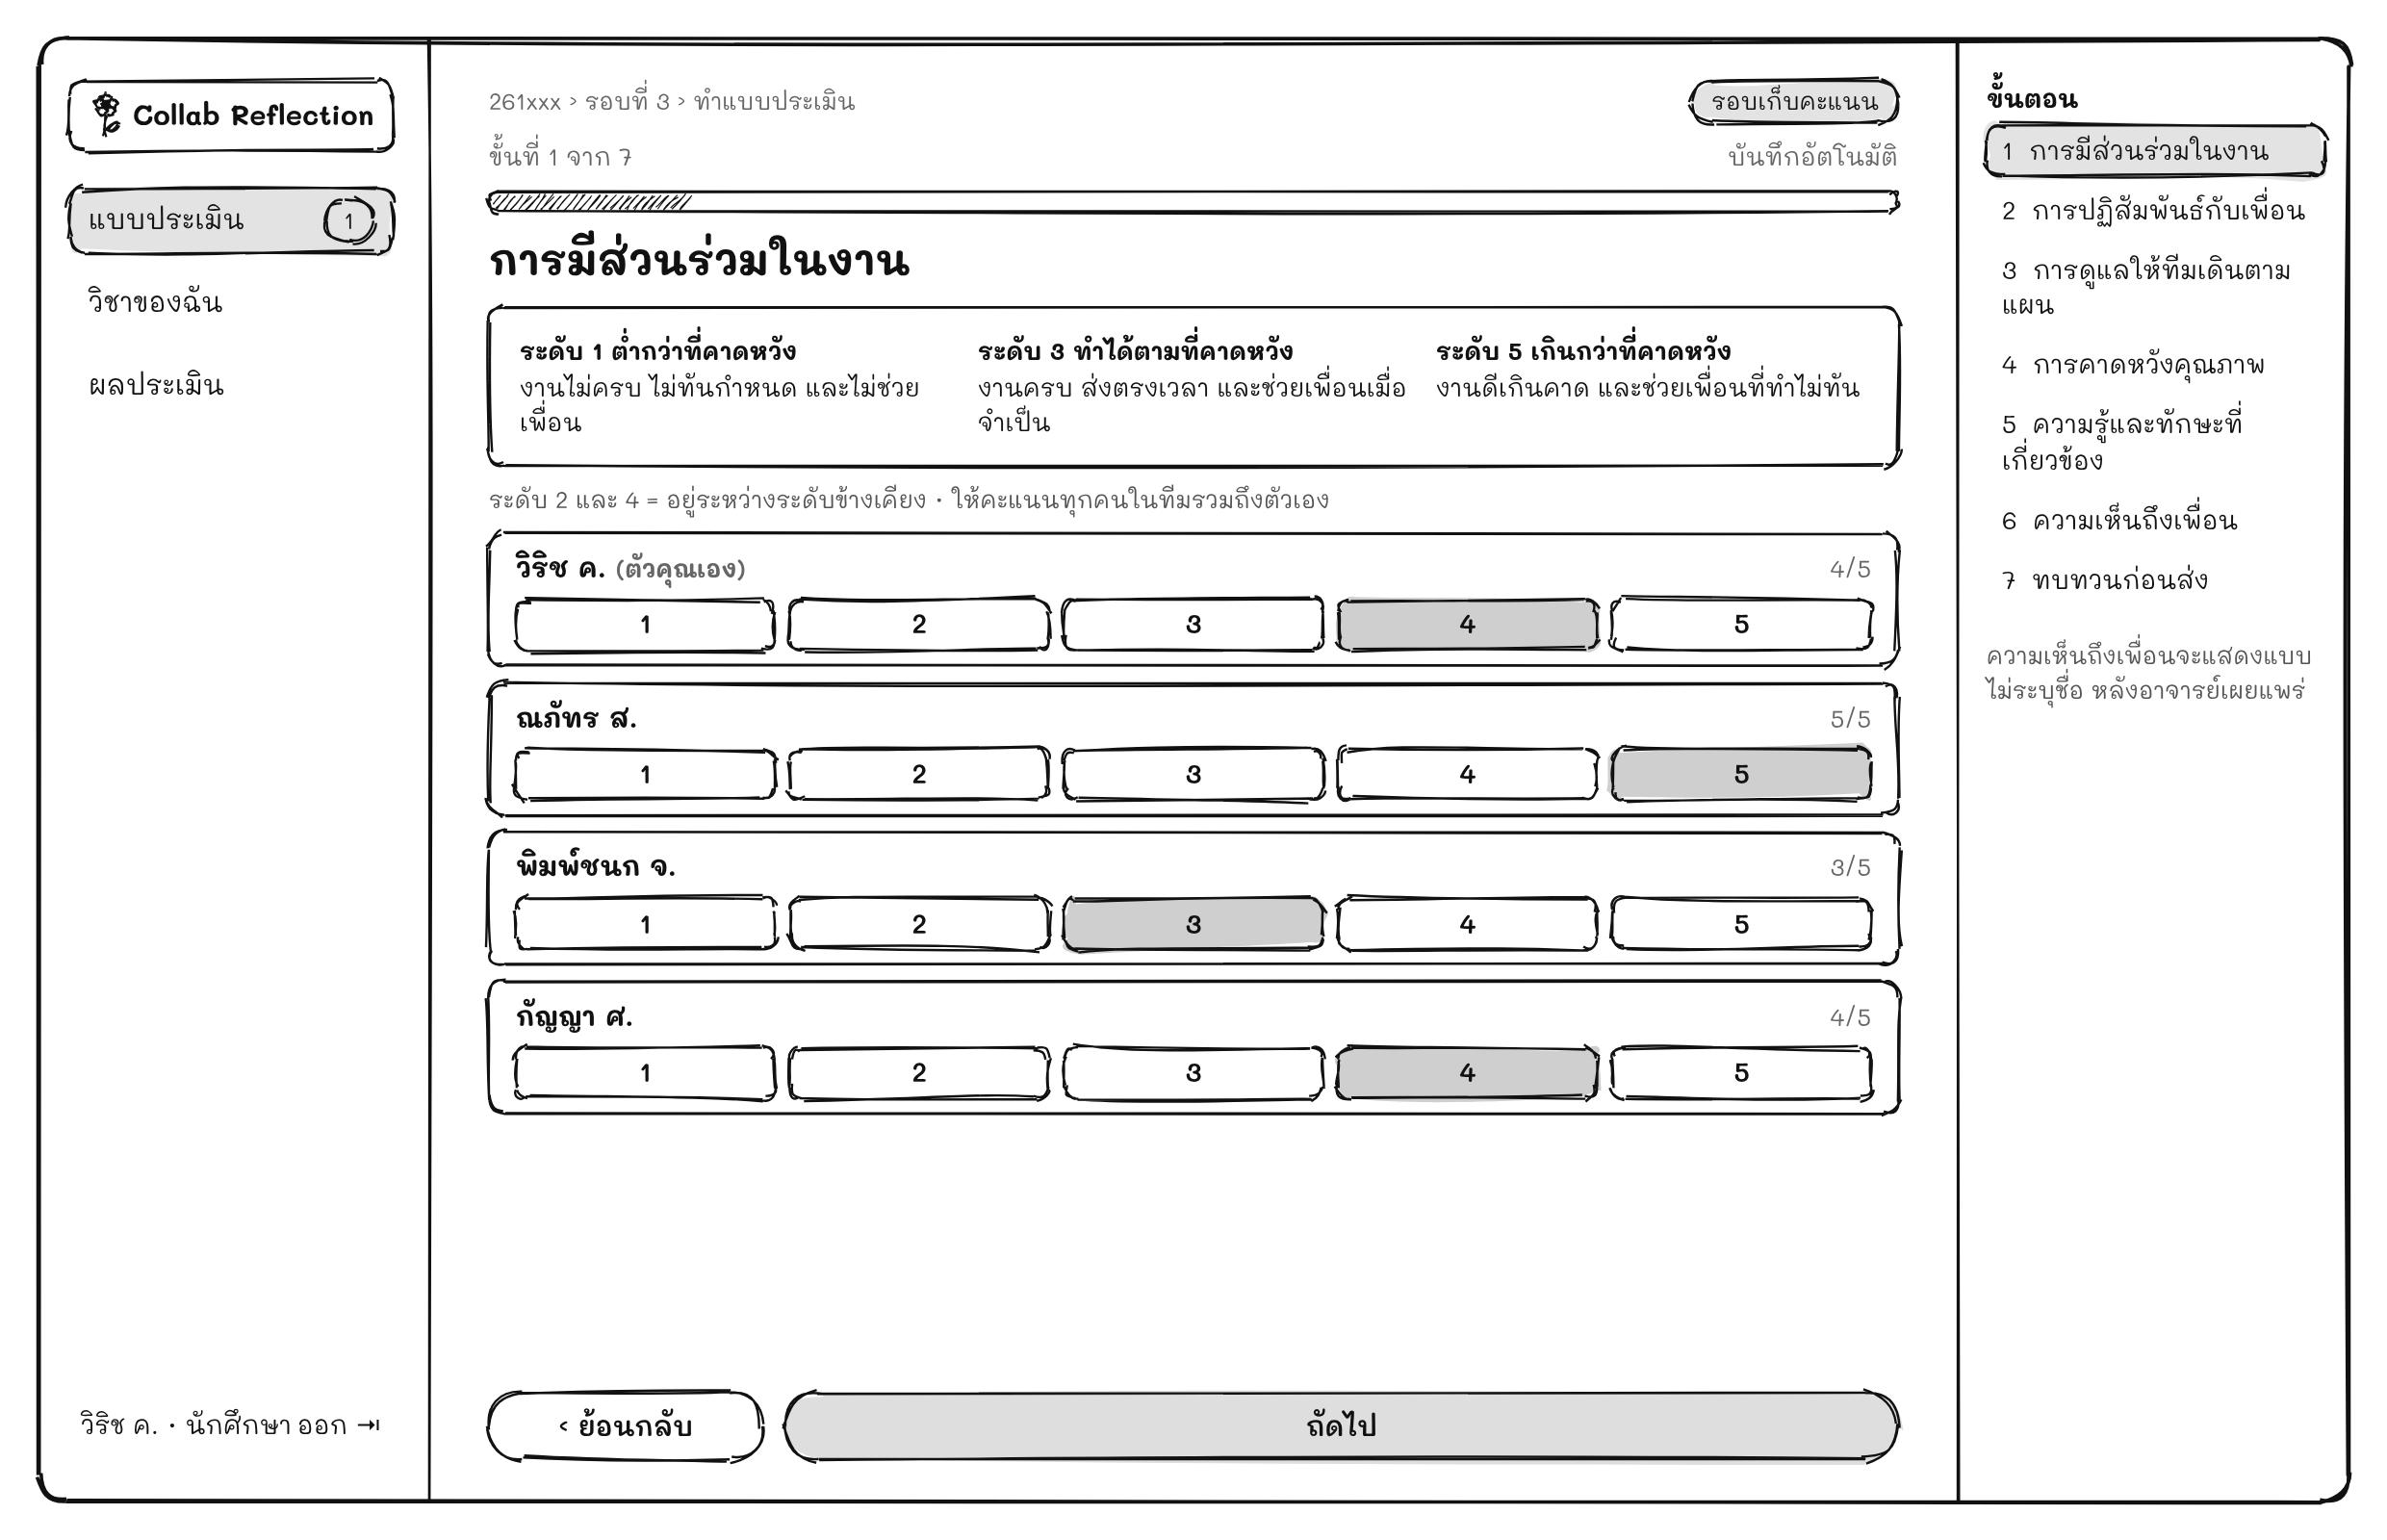
\includegraphics[width=0.85\textwidth]{figures/ch3/fig3-8-student-rating.png}}{\fbox{\parbox{0.8\textwidth}{\centering\vspace{2cm}[วางไฟล์ figures/ch3/fig3-8-student-rating.png]\vspace{2cm}}}}
\caption{หน้าให้คะแนนรายด้าน}\label{fig:ch3-8}
\end{figure}

ขั้นความเห็นถึงเพื่อนใช้แนวคิด ``ให้ดอกไม้ เติมปุ๋ย'' ดอกไม้คือสิ่งที่เพื่อนทำดีอยู่แล้วและควรได้รับคำชมเพื่อให้เติบโตต่อ ส่วนปุ๋ยเป็นสิ่งที่ช่วยให้เพื่อนเติบโตในงานถัดไป หน้าจอมีกล่องอธิบายพร้อมตัวอย่างการเขียน และภาพประกอบการเติบโตจากต้นอ่อนเป็นดอกไม้ ดังรูปที่~\ref{fig:ch3-9}

\begin{figure}[htbp]
\centering
\IfFileExists{figures/ch3/fig3-9-student-comments.png}{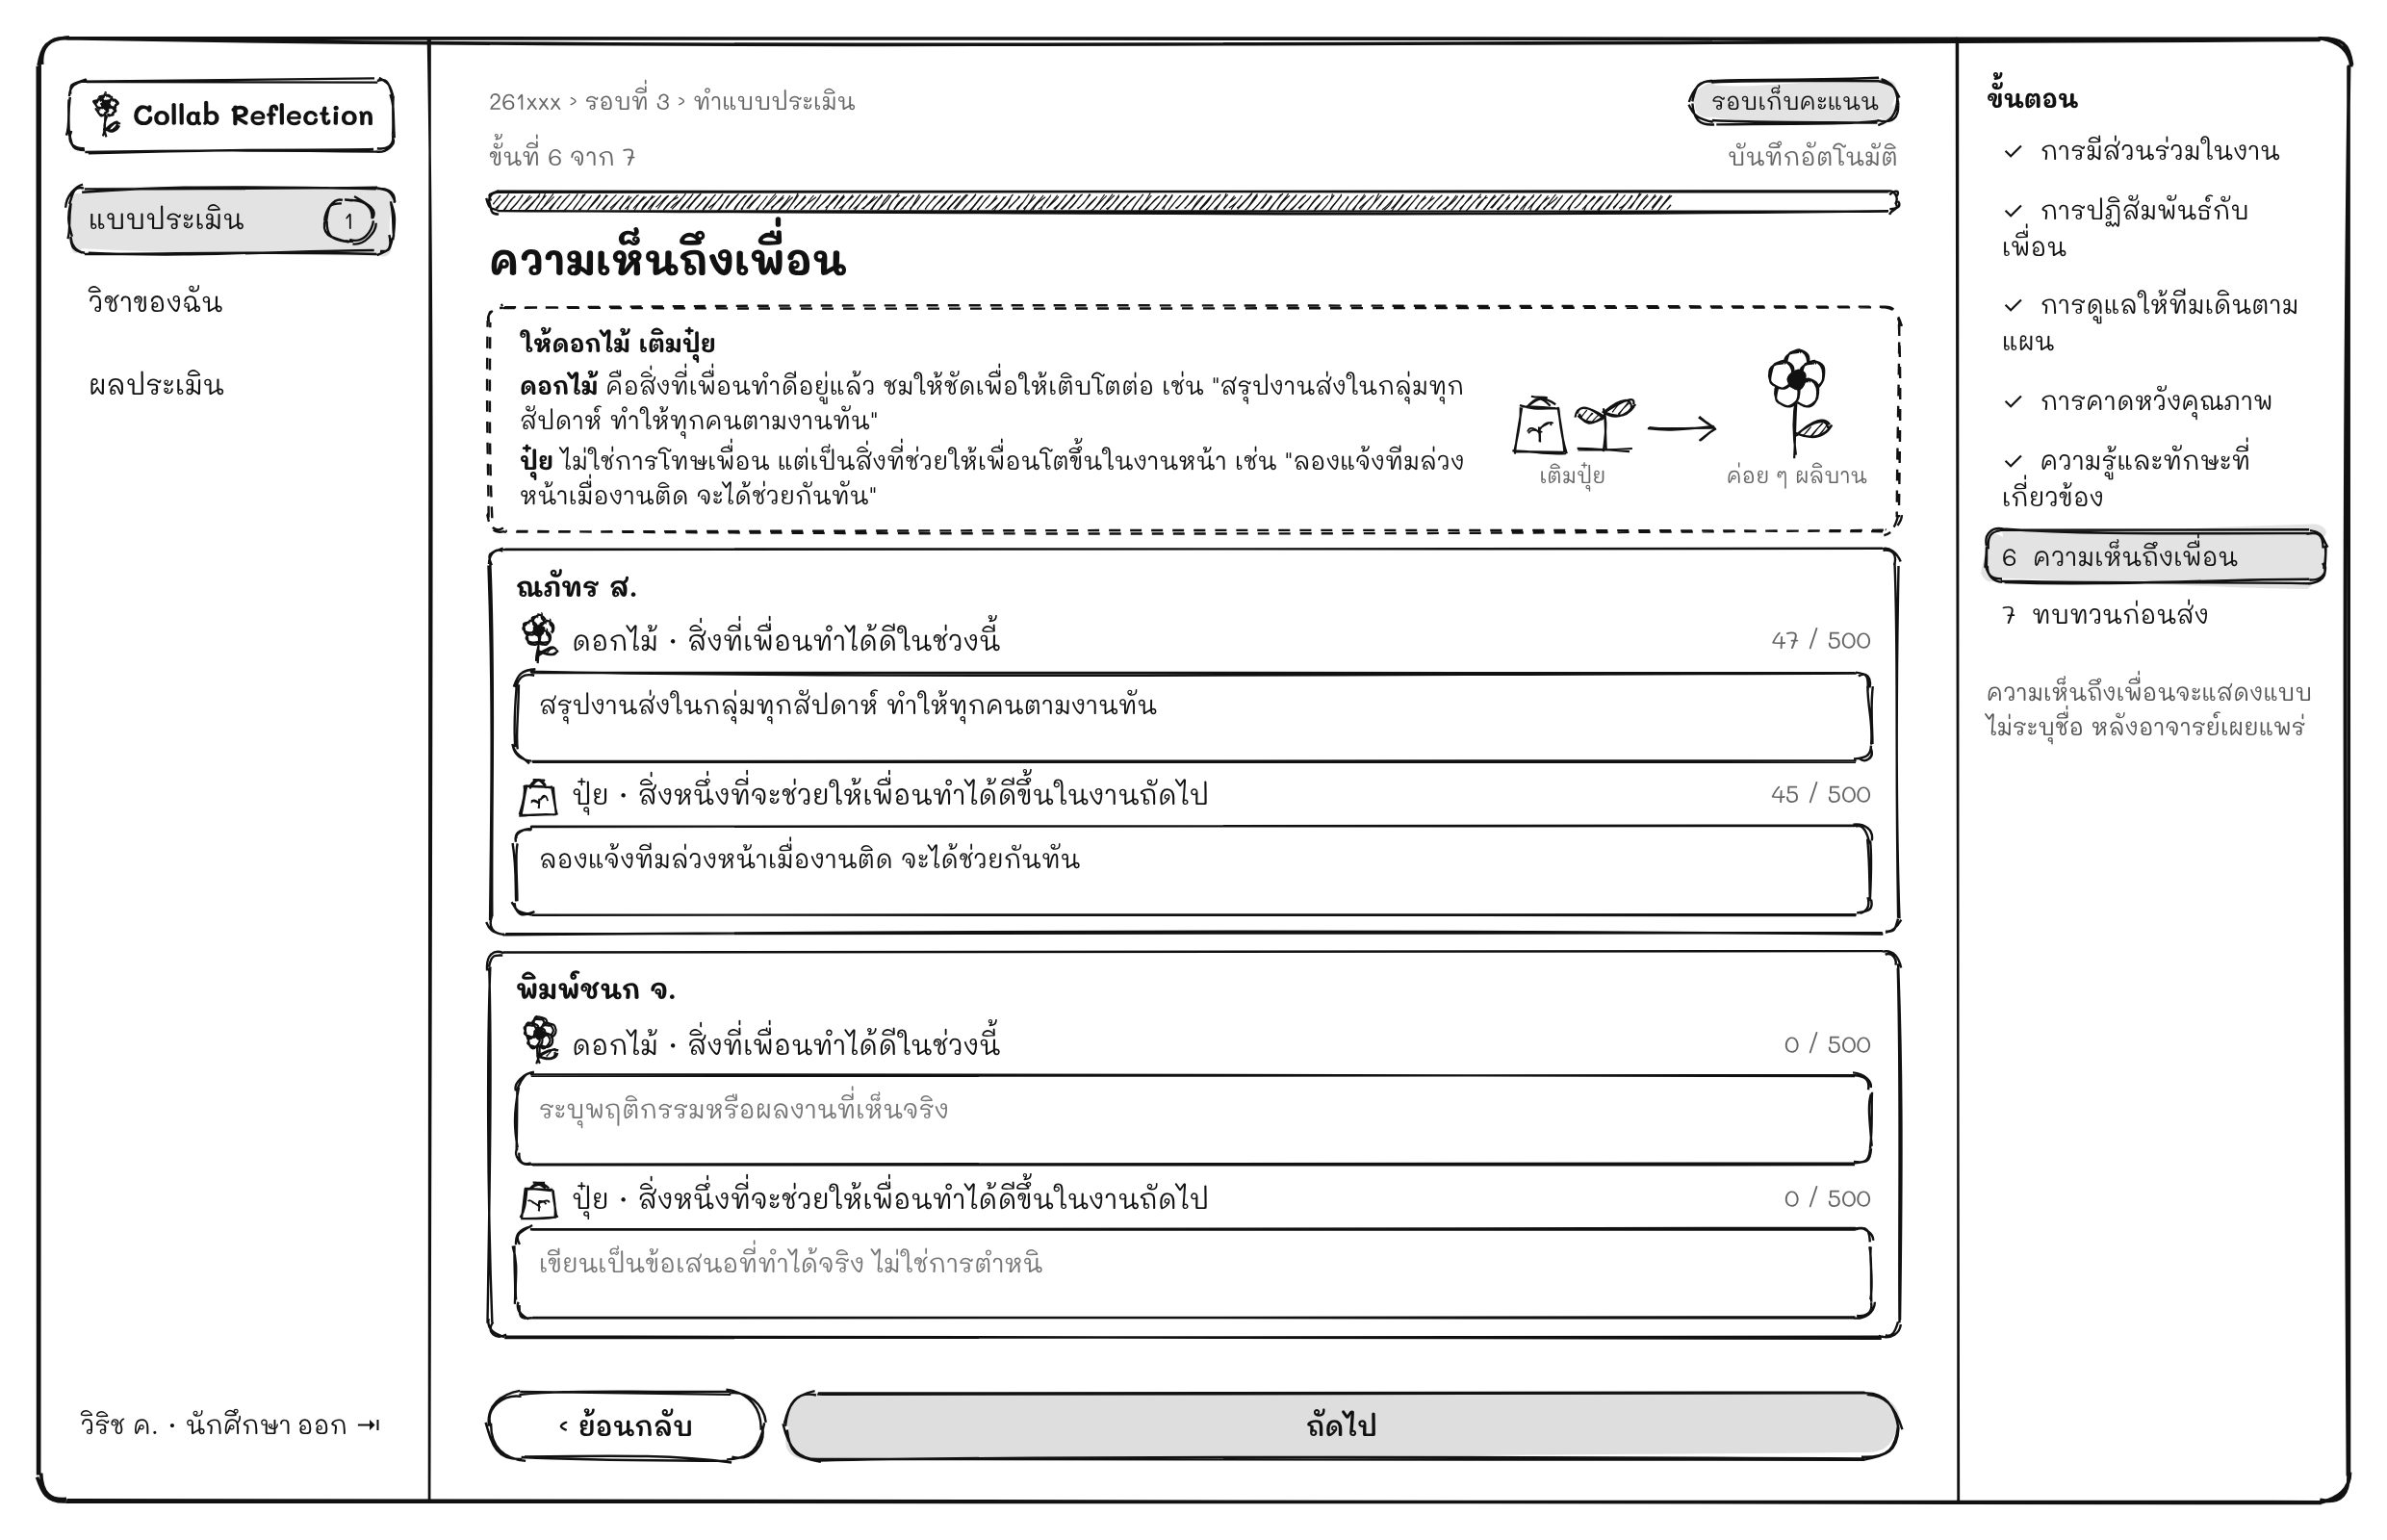
\includegraphics[width=0.85\textwidth]{figures/ch3/fig3-9-student-comments.png}}{\fbox{\parbox{0.8\textwidth}{\centering\vspace{2cm}[วางไฟล์ figures/ch3/fig3-9-student-comments.png]\vspace{2cm}}}}
\caption{หน้าเขียนความเห็นแบบดอกไม้และปุ๋ย}\label{fig:ch3-9}
\end{figure}

หน้าดูผลแสดงคะแนนรายด้านด้วยแผนภูมิเรดาร์ เปรียบเทียบค่าเฉลี่ยที่เพื่อนประเมินกับคะแนนที่ประเมินตนเอง แสดงดอกไม้และปุ๋ยที่ได้รับ ข้อเสนอแนะจากอาจารย์ และมีปุ่มขอความช่วยเหลือสำหรับนักศึกษาที่รู้สึกไม่สบายใจ ดังรูปที่~\ref{fig:ch3-10}

\begin{figure}[htbp]
\centering
\IfFileExists{figures/ch3/fig3-10-student-result.png}{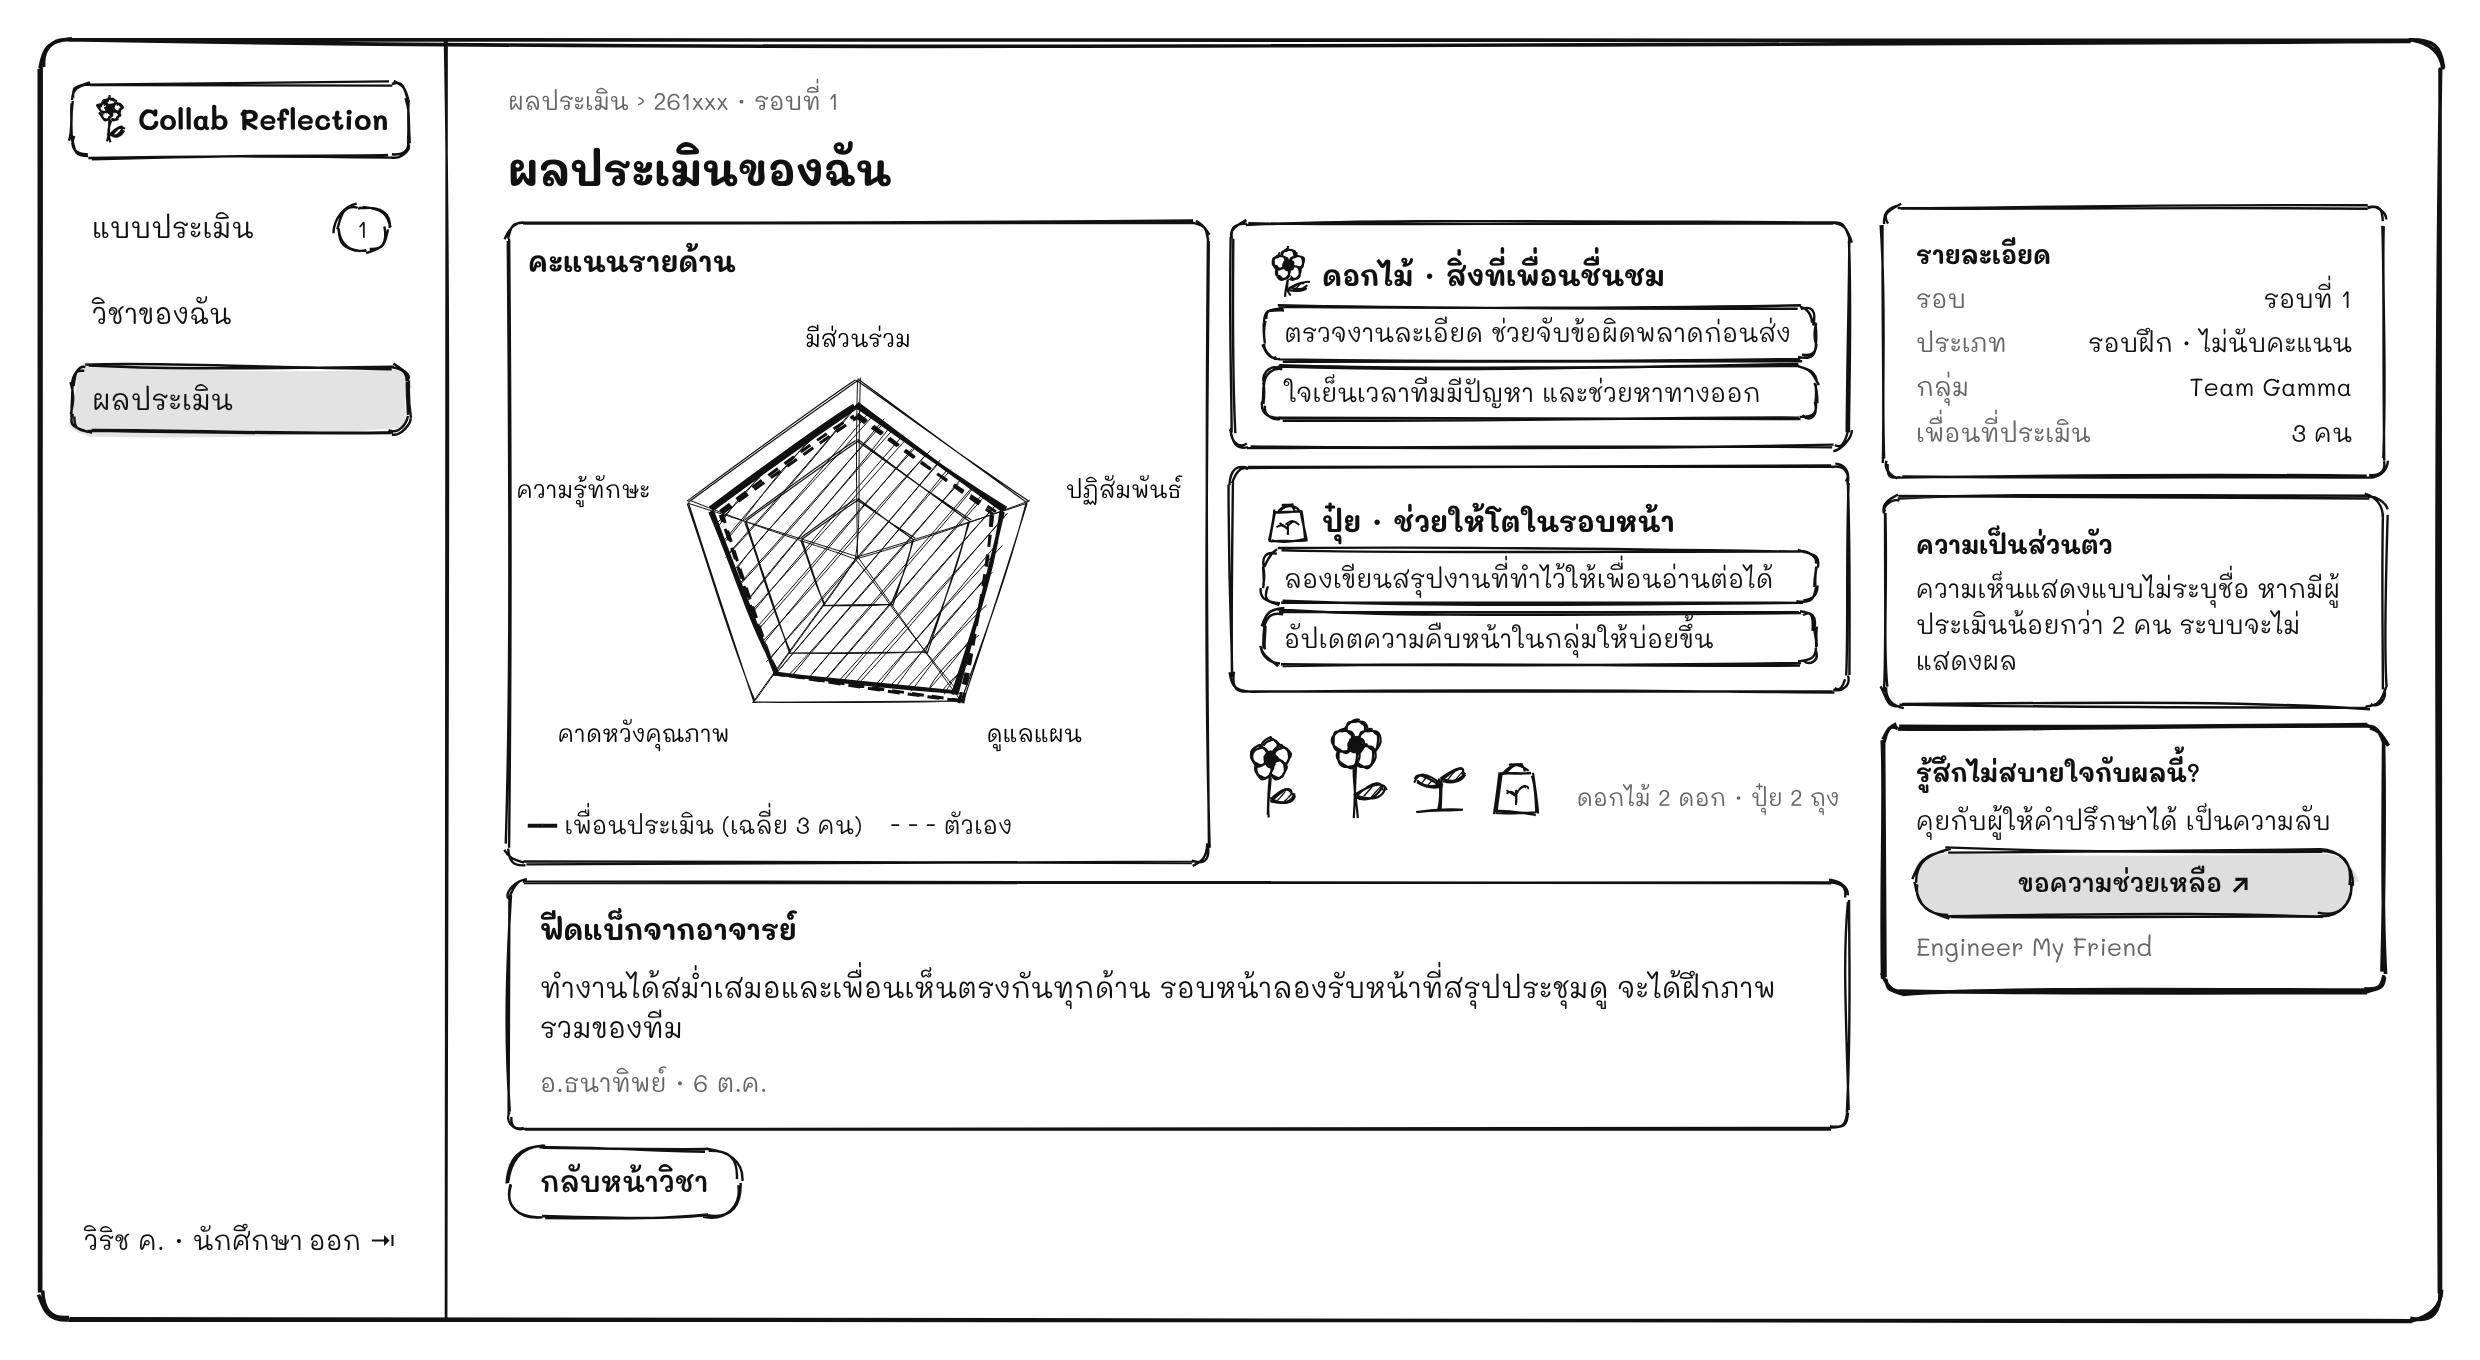
\includegraphics[width=\textwidth]{figures/ch3/fig3-10-student-result.png}}{\fbox{\parbox{0.8\textwidth}{\centering\vspace{2cm}[วางไฟล์ figures/ch3/fig3-10-student-result.png]\vspace{2cm}}}}
\caption{หน้าดูผลการประเมินของนักศึกษา}\label{fig:ch3-10}
\end{figure}

\subsection{หน้าจอฝั่งอาจารย์}\label{sec:3.8.3}

หน้าสมาชิกใช้นำเข้ารายชื่อนักศึกษาจากไฟล์ CSV จัดกลุ่ม และตรวจว่านักศึกษาคนใดยังไม่ยอมรับข้อตกลง PDPA ดังรูปที่~\ref{fig:ch3-11}

\begin{figure}[htbp]
\centering
\IfFileExists{figures/ch3/fig3-11-instructor-members.png}{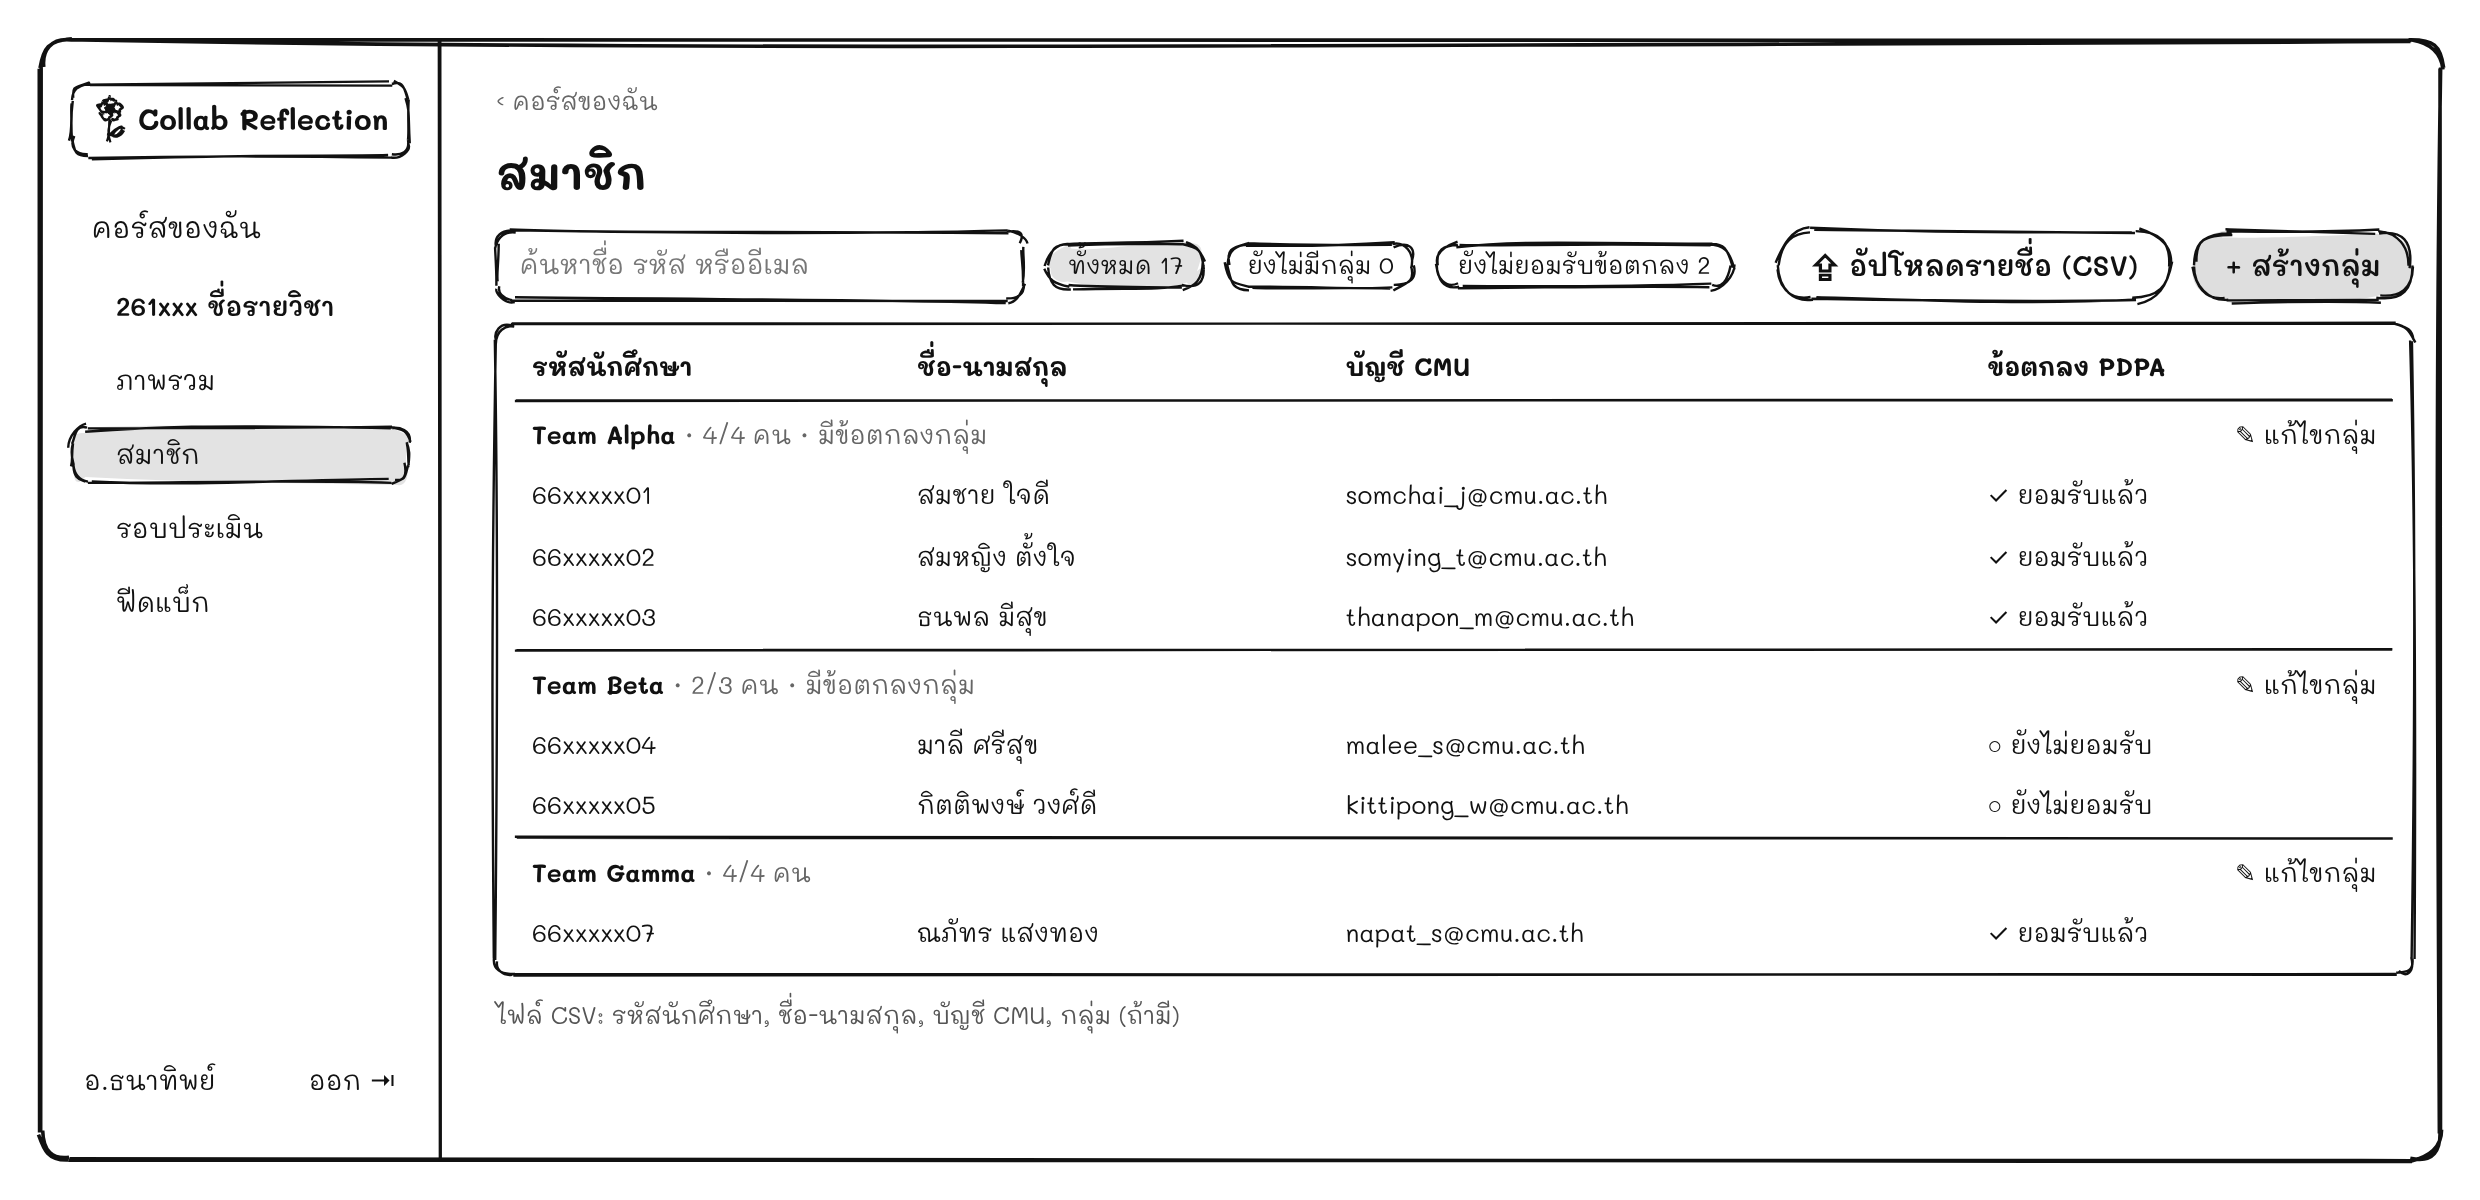
\includegraphics[width=\textwidth]{figures/ch3/fig3-11-instructor-members.png}}{\fbox{\parbox{0.8\textwidth}{\centering\vspace{2cm}[วางไฟล์ figures/ch3/fig3-11-instructor-members.png]\vspace{2cm}}}}
\caption{หน้าจัดการสมาชิกและกลุ่ม}\label{fig:ch3-11}
\end{figure}

หน้ารอบประเมินแสดงรอบทั้งหมดของรายวิชา เมื่อเพิ่มรอบใหม่ อาจารย์ต้องเลือกประเภทของรอบ (รอบฝึกหรือรอบเก็บคะแนน) และกำหนดช่วงเวลาเปิดปิด ดังรูปที่~\ref{fig:ch3-12}

\begin{figure}[htbp]
\centering
\IfFileExists{figures/ch3/fig3-12-instructor-rounds.png}{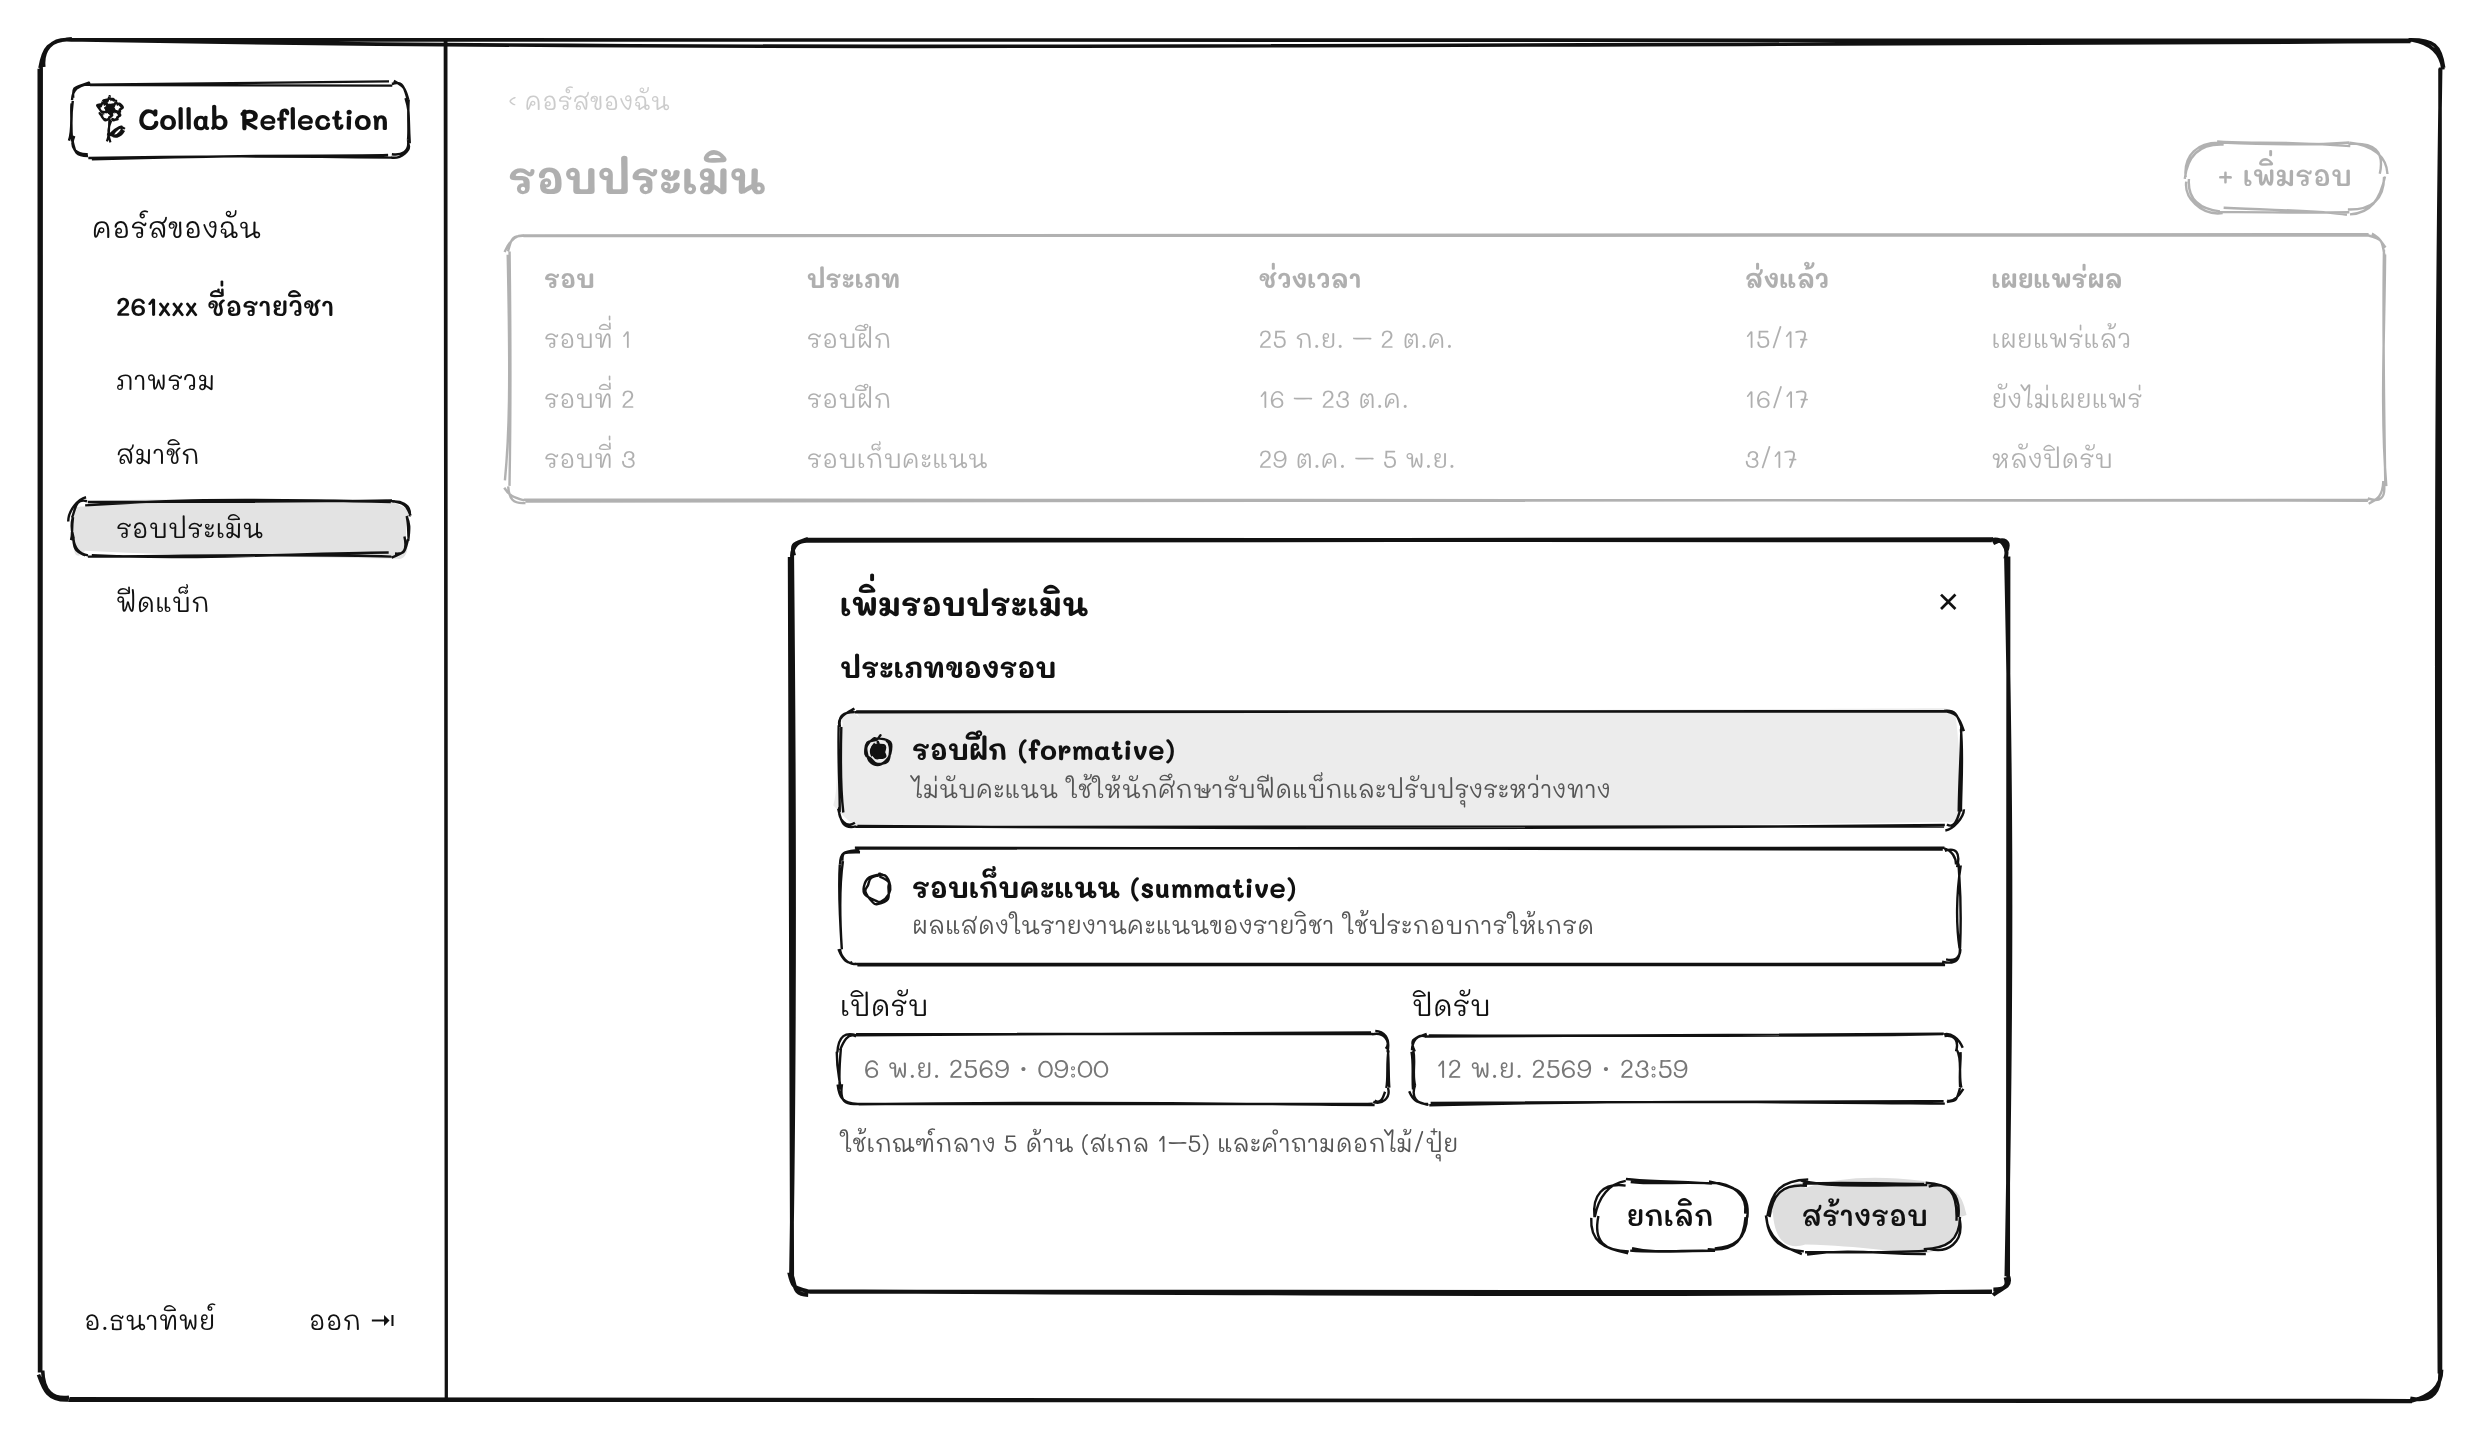
\includegraphics[width=\textwidth]{figures/ch3/fig3-12-instructor-rounds.png}}{\fbox{\parbox{0.8\textwidth}{\centering\vspace{2cm}[วางไฟล์ figures/ch3/fig3-12-instructor-rounds.png]\vspace{2cm}}}}
\caption{หน้าเพิ่มรอบประเมิน}\label{fig:ch3-12}
\end{figure}

แดชบอร์ดแสดงภาพรวมของรอบที่เลือก จำนวนผู้ส่ง แผนภาพเปรียบเทียบคะแนนที่ประเมินตนเองกับที่เพื่อนประเมิน และสัญญาณที่ควรดูของแต่ละทีม ดังรูปที่~\ref{fig:ch3-13}

\begin{figure}[htbp]
\centering
\IfFileExists{figures/ch3/fig3-13-instructor-overview.png}{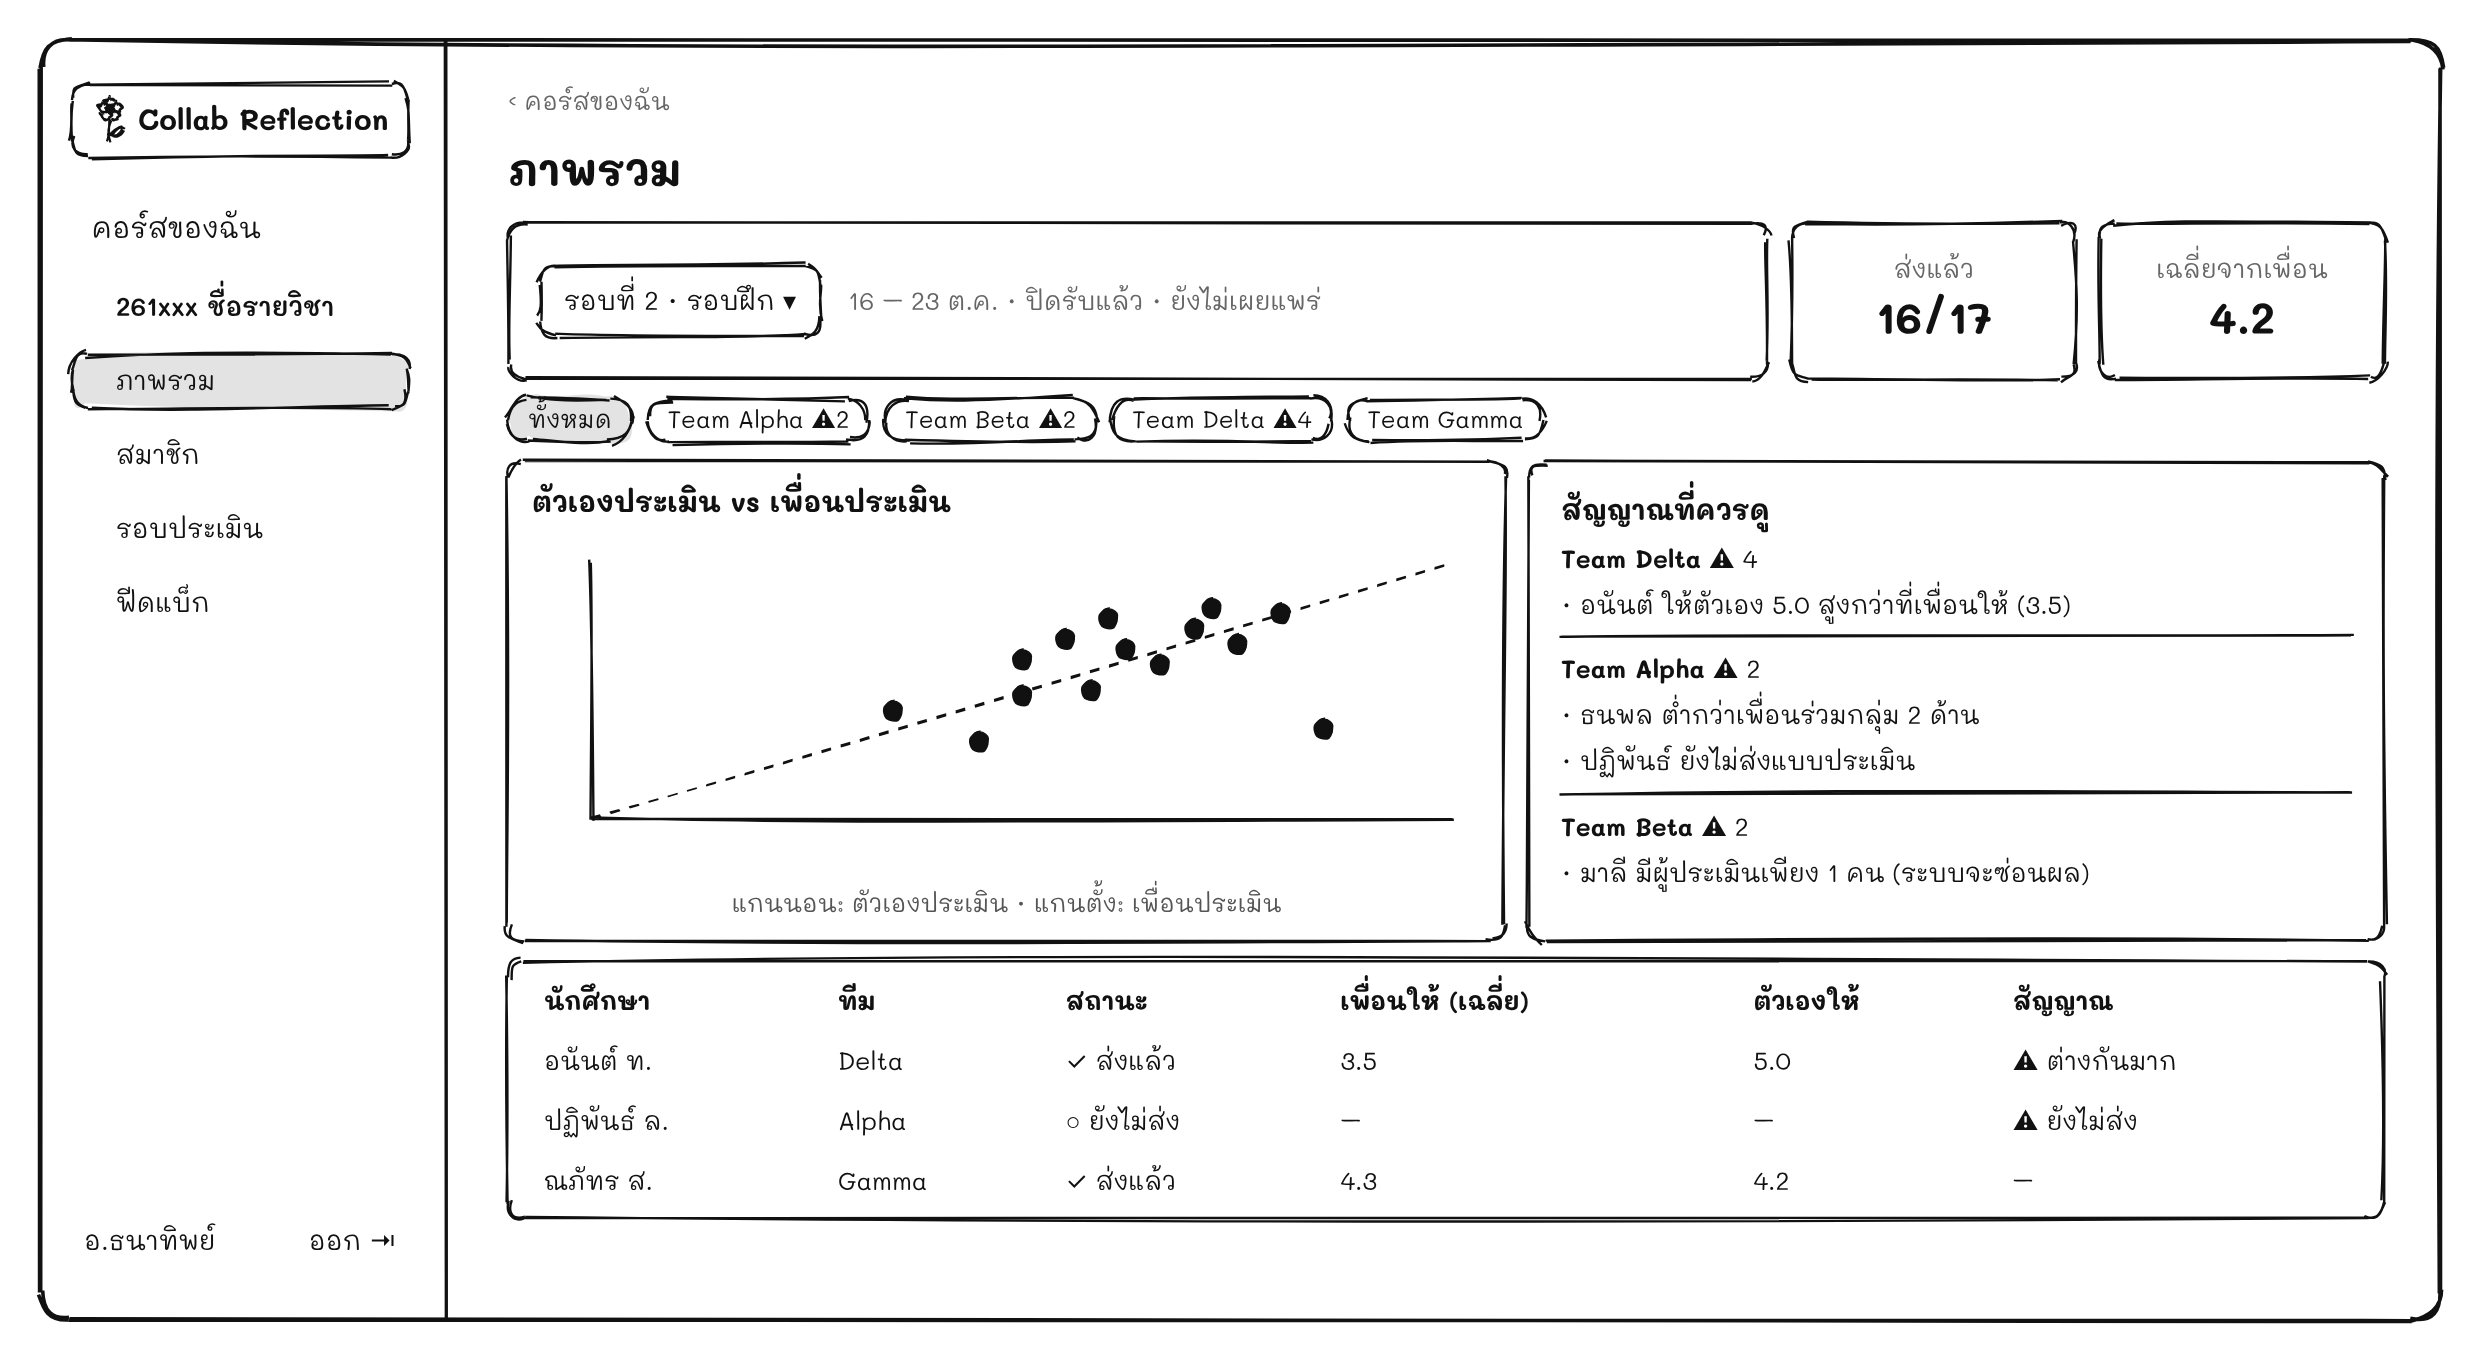
\includegraphics[width=\textwidth]{figures/ch3/fig3-13-instructor-overview.png}}{\fbox{\parbox{0.8\textwidth}{\centering\vspace{2cm}[วางไฟล์ figures/ch3/fig3-13-instructor-overview.png]\vspace{2cm}}}}
\caption{แดชบอร์ดของอาจารย์}\label{fig:ch3-13}
\end{figure}

หน้าภาพรวมแสดงผลของนักศึกษาทีละคน ให้อาจารย์อ่านดอกไม้และปุ๋ยจากเพื่อน เลือกว่านักศึกษาจะเห็นความเห็นของเพื่อนตามจริงหรือเฉพาะข้อสรุปของอาจารย์ เขียนข้อเสนอแนะ และกดเผยแพร่ผลของทั้งรอบ ดังรูปที่~\ref{fig:ch3-14}

\begin{figure}[htbp]
\centering
\IfFileExists{figures/ch3/fig3-14-instructor-feedback.png}{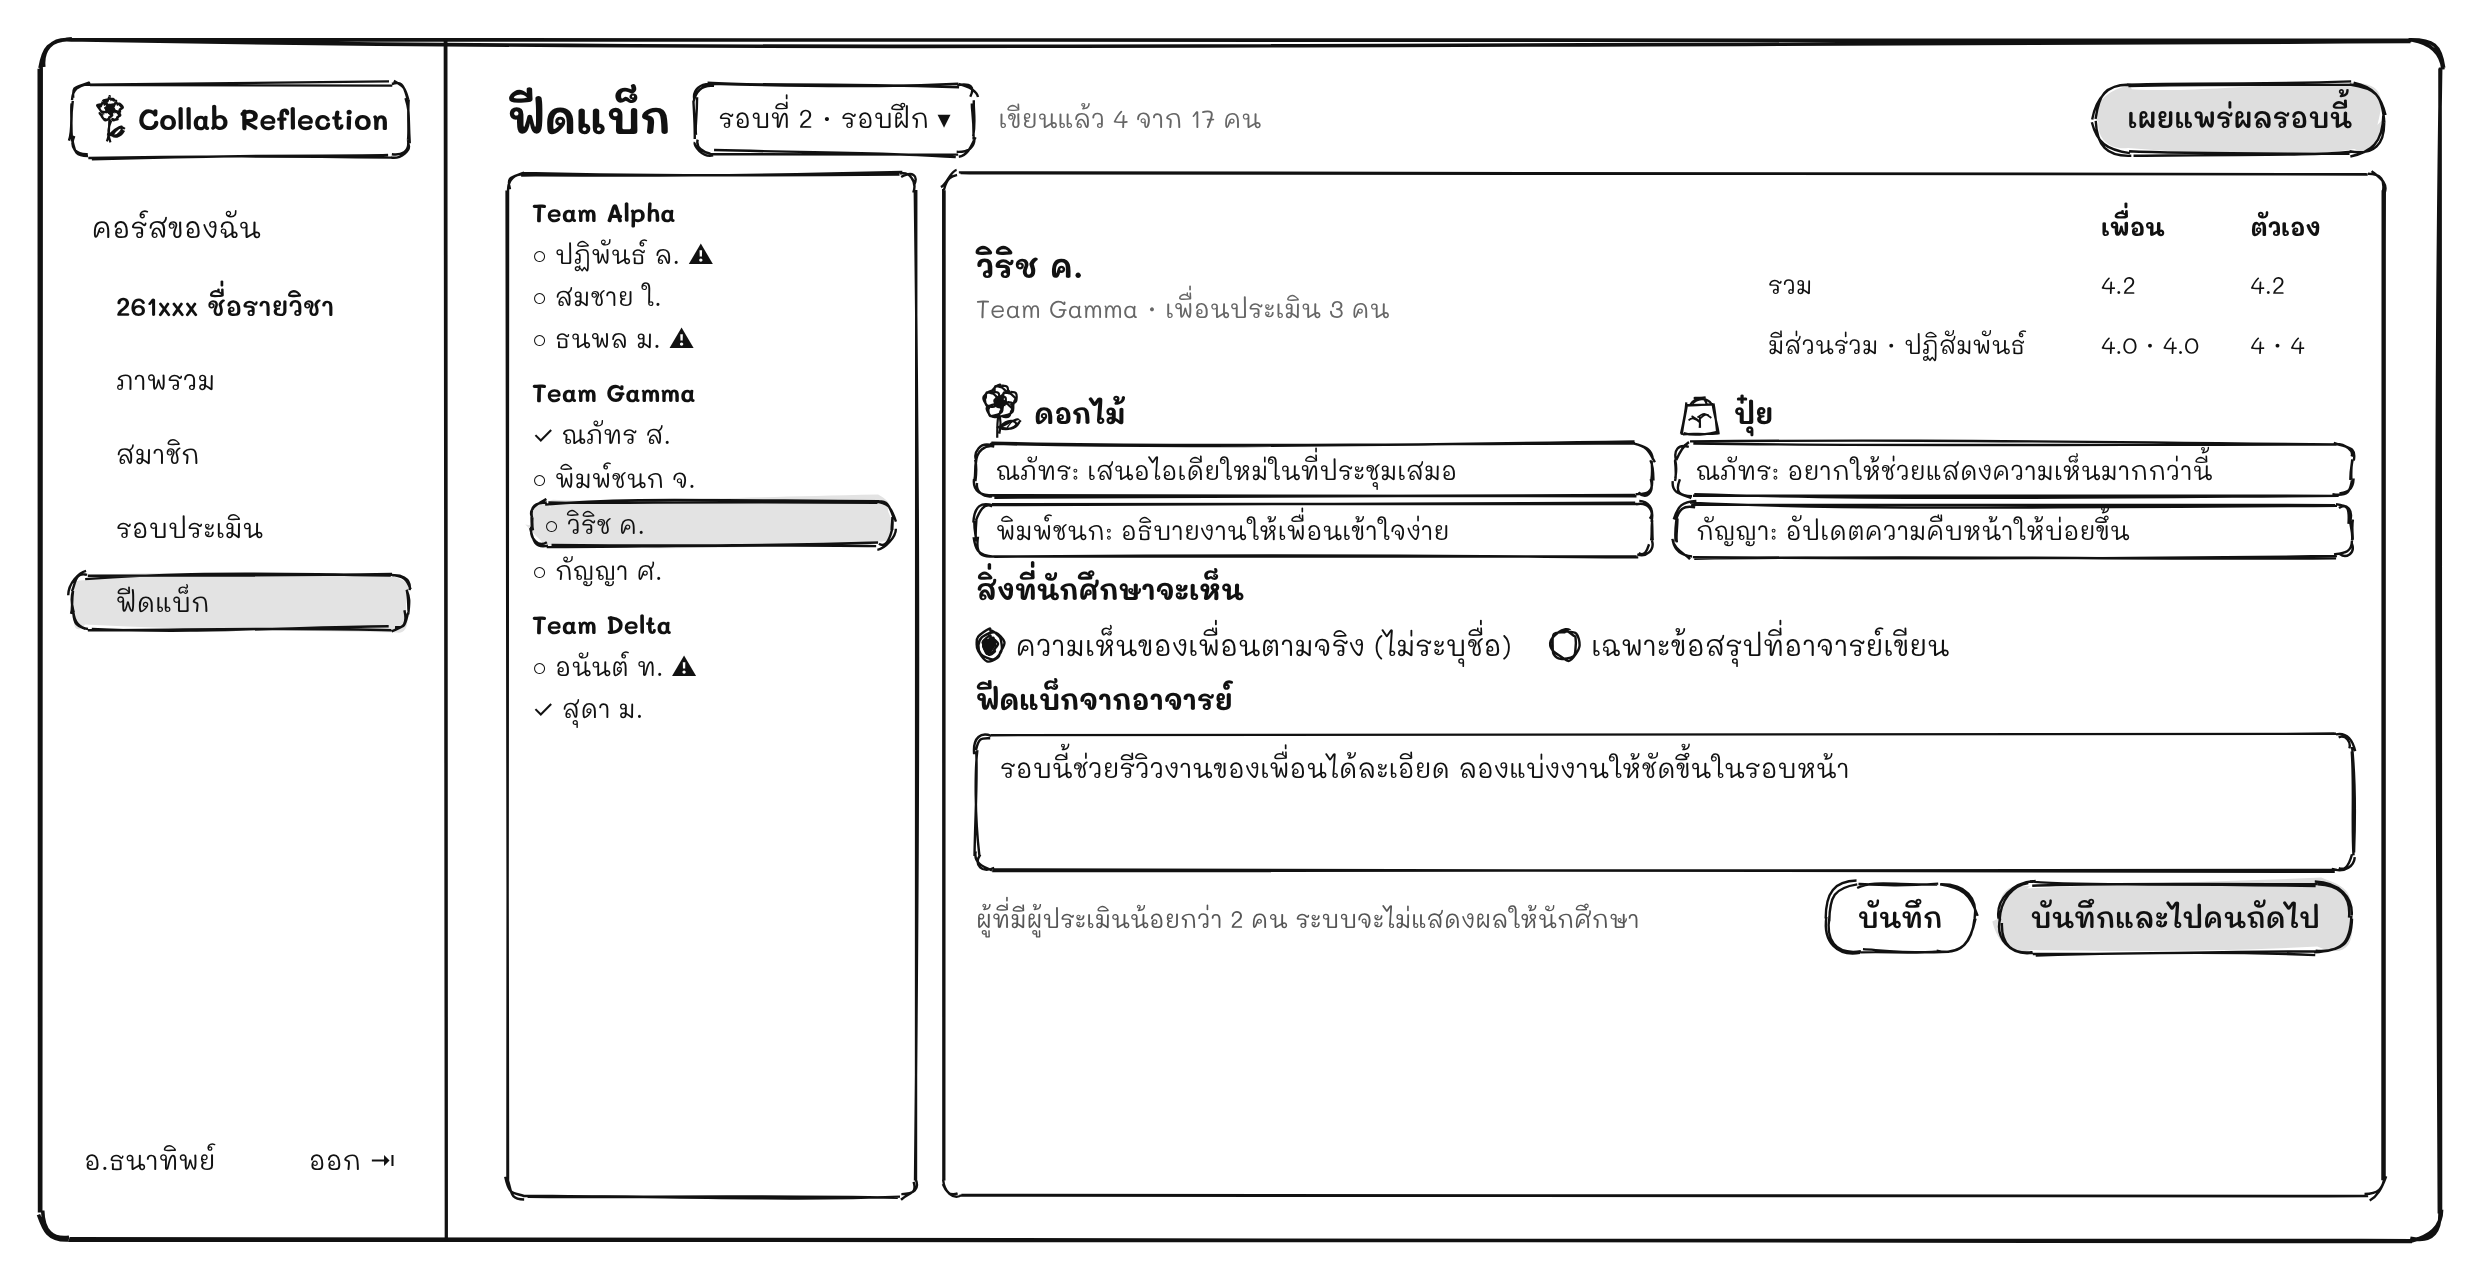
\includegraphics[width=\textwidth]{figures/ch3/fig3-14-instructor-feedback.png}}{\fbox{\parbox{0.8\textwidth}{\centering\vspace{2cm}[วางไฟล์ figures/ch3/fig3-14-instructor-feedback.png]\vspace{2cm}}}}
\caption{หน้าตรวจทานและเผยแพร่ผล}\label{fig:ch3-14}
\end{figure}

\section{ความปลอดภัยและการคุ้มครองข้อมูลส่วนบุคคล}\label{sec:3.9}

\subsection{ความปลอดภัยของระบบ}\label{sec:3.9.1}

\begin{itemize}
  \item เข้าสู่ระบบด้วยบัญชี CMU เท่านั้น และระบบไม่เก็บรหัสผ่าน
  \item ตรวจสิทธิ์ตามบทบาทในทุก API และบังคับกฎการปกปิดตัวตนที่ฝั่งเซิร์ฟเวอร์
  \item เข้ารหัสการสื่อสารด้วย HTTPS และใช้คุกกี้เซสชันแบบ HttpOnly และ Secure
  \item ตรวจสอบข้อมูลขาเข้าทุกครั้ง และใช้ ORM ที่สร้างคำสั่ง SQL แบบมีพารามิเตอร์ เพื่อป้องกัน SQL injection
  \item แบบประเมินที่ส่งแล้วแก้ไขไม่ได้ เพื่อป้องกันการเปลี่ยนคะแนนย้อนหลัง
\end{itemize}

\subsection{การคุ้มครองข้อมูลส่วนบุคคล}\label{sec:3.9.2}

ระบบออกแบบตามหลักของพระราชบัญญัติคุ้มครองข้อมูลส่วนบุคคล พ.ศ. 2562~\cite{pdpa2562} ได้แก่ เก็บข้อมูลเท่าที่จำเป็นต่อการประเมินงานกลุ่มเท่านั้น แจ้งก่อนใช้ว่าเก็บข้อมูลอะไร ใครเห็น และเก็บนานเท่าใด และให้เจ้าของข้อมูลใช้สิทธิ์ขอดู แก้ไข หรือลบข้อมูลได้

เพื่อไม่ให้นักศึกษาที่ไม่ยินยอมบางเรื่องต้องหลุดออกจากระบบจนเก็บคะแนนไม่ได้ ข้อตกลงจึงแบ่งเป็นส่วนจำเป็นและส่วนทางเลือก ดังตารางที่~\ref{tab:ch3-9} ทั้งนี้ คณะผู้จัดทำจะยืนยันระยะเวลาเก็บข้อมูลและฐานทางกฎหมายของการประมวลผลส่วนจำเป็นกับหน่วยงานที่ดูแลการคุ้มครองข้อมูลส่วนบุคคลของมหาวิทยาลัยก่อนใช้งานจริง

\begin{xltabular}{\textwidth}{|P{0.14\textwidth}|Y|Y|}
\caption{การแบ่งข้อตกลงการใช้ข้อมูลส่วนบุคคล}\label{tab:ch3-9}\\
\hline \textbf{ส่วน} & \textbf{ข้อมูลและการใช้งาน} & \textbf{หากไม่ยินยอม} \\ \hline
\endfirsthead
\multicolumn{3}{r}{\small (ต่อ)}\\ \hline \textbf{ส่วน} & \textbf{ข้อมูลและการใช้งาน} & \textbf{หากไม่ยินยอม} \\ \hline
\endhead
ส่วนจำเป็น & ข้อมูลบัญชี CMU รายวิชาและกลุ่มที่สังกัด คะแนนและความเห็นที่ใช้ในการประเมินของรายวิชา & ต้องรับทราบจึงจะใช้ระบบได้ เพราะเป็นข้อมูลขั้นต่ำของการประเมิน \\ \hline
ส่วนทางเลือก 1 & ส่งข้อความที่เขียนให้ปัญญาประดิษฐ์ (AI) ประมวลผล (เฟสที่ 2) & ใช้ระบบและได้คะแนนตามปกติ แต่ข้อความของผู้นั้นจะไม่ถูกส่งให้ปัญญาประดิษฐ์ (AI) \\ \hline
ส่วนทางเลือก 2 & นำข้อมูลแบบไม่ระบุตัวตนไปใช้พัฒนาระบบและในงานวิจัย & ใช้ระบบและได้คะแนนตามปกติ แต่ข้อมูลของผู้นั้นจะไม่ถูกนำไปใช้ \\ \hline
\end{xltabular}

\subsection{การดูแลความรู้สึกของผู้ใช้}\label{sec:3.9.3}

ข้อเสนอแนะจากเพื่อนอาจกระทบความรู้สึกของผู้รับได้แม้ผ่านการกลั่นกรองแล้ว ระบบจึงลดโอกาสเกิดความคิดเห็นที่ทำร้ายจิตใจตั้งแต่ต้นทาง ด้วยคำถามแบบดอกไม้และปุ๋ย คำแนะนำการเขียน และการตรวจทานของอาจารย์ก่อนเผยแพร่ และที่หน้าดูผลมีปุ่มขอความช่วยเหลือที่เชื่อมไปยังช่องทางให้คำปรึกษา เช่น โครงการ Entaneer Mind Friend สำหรับนักศึกษาที่รู้สึกไม่สบายใจ

\section{แผนการประเมินระบบและตัวชี้วัดความสำเร็จ}\label{sec:3.10}

การประเมินระบบอยู่ในระยะที่ 4 ของการดำเนินงาน แบ่งเป็นการตรวจสอบว่าระบบทำงานถูกต้องตามที่ออกแบบ (verification) และการยืนยันว่าระบบแก้ปัญหาของผู้ใช้ได้จริง (validation)

\subsection{การตรวจสอบความถูกต้องของระบบ}\label{sec:3.10.1}

\begin{itemize}
  \item Unit test ด้วย Vitest สำหรับตรรกะสำคัญ เช่น การคำนวณค่าเฉลี่ยรายด้าน เงื่อนไขซ่อนผลเมื่อผู้ประเมินไม่ถึง 2 คน และเงื่อนไขสัญญาณเตือน
  \item Integration test ของ API ทุกเส้นทาง รวมถึงทดสอบว่านักศึกษาเรียกดูข้อมูลที่ตนไม่มีสิทธิ์ไม่ได้
  \item End-to-end test ด้วย Cypress สำหรับขั้นตอนหลัก ได้แก่ นักศึกษาส่งแบบประเมิน และอาจารย์ตรวจทานและเผยแพร่ผล
  \item ทดสอบโหลดด้วยจำนวนผู้ใช้เทียบเท่าหนึ่งรายวิชา
  \item ส่วน AI (เฟสที่ 2): วัดความสอดคล้องระหว่างผลการตรวจโทนของโมเดลกับการติดป้ายกำกับโดยคน บนชุดข้อความภาษาไทยตัวอย่าง
\end{itemize}

\subsection{การนำร่องใช้งานจริง}\label{sec:3.10.2}

คณะผู้จัดทำจะนำระบบไปทดลองใช้ในรายวิชาที่มีการทำงานกลุ่มระยะยาวของภาควิชาวิศวกรรมคอมพิวเตอร์อย่างน้อย 1 รายวิชา โดยมีรอบฝึกอย่างน้อย 1 รอบและรอบเก็บคะแนน 1 รอบ หลังใช้งานจะเก็บแบบสอบถาม System Usability Scale (SUS)~\cite{brooke1996sus} จากทั้งอาจารย์และนักศึกษา และสัมภาษณ์อาจารย์ผู้สอนเรื่องภาระงานและประโยชน์ที่ได้รับ เพื่อนำไปพัฒนาในระยะถัดไป

\subsection{ตัวชี้วัดความสำเร็จ}\label{sec:3.10.3}

ตัวชี้วัดความสำเร็จของโครงงานแสดงในตารางที่~\ref{tab:ch3-10}

\begin{xltabular}{\textwidth}{|P{0.14\textwidth}|P{0.2\textwidth}|Y|P{0.15\textwidth}|}
\caption{ตัวชี้วัดความสำเร็จของโครงงาน}\label{tab:ch3-10}\\
\hline \textbf{ด้าน} & \textbf{ตัวชี้วัด} & \textbf{เป้าหมาย} & \textbf{วิธีวัด} \\ \hline
\endfirsthead
\multicolumn{4}{r}{\small (ต่อ)}\\ \hline \textbf{ด้าน} & \textbf{ตัวชี้วัด} & \textbf{เป้าหมาย} & \textbf{วิธีวัด} \\ \hline
\endhead
ความถูกต้องของระบบ & กรณีทดสอบของฟีเจอร์ระยะที่ 1 & ผ่านทั้งหมด & Vitest และ Cypress \\ \hline
การใช้งานจริง & จำนวนรายวิชานำร่อง & อย่างน้อย 1 รายวิชา และ 2 รอบประเมิน & บันทึกการใช้งานในระบบ \\ \hline
การรองรับผู้ใช้ & จำนวนผู้ใช้ที่ใช้งานพร้อมกันได้ & ประมาณ 90 คนต่อรายวิชา ตามสัดส่วนนักศึกษาต่ออาจารย์ในรายวิชาเป้าหมาย & ทดสอบโหลด \\ \hline
การมีส่วนร่วม & อัตราการส่งแบบประเมินต่อรอบ & อย่างน้อยร้อยละ 80 & ข้อมูลในระบบ \\ \hline
ความง่ายในการใช้งาน & คะแนน SUS & อย่างน้อย 68 คะแนน ซึ่งเป็นค่าเฉลี่ยอ้างอิงทั่วไป~\cite{sauro2011sus} ทั้งฝั่งอาจารย์และนักศึกษา & แบบสอบถาม SUS \\ \hline
ภาระงานของอาจารย์ & เวลาที่ใช้ตรวจทานและเผยแพร่ผลต่อหนึ่งกลุ่ม & น้อยกว่าวิธีเดิมที่อาจารย์ใช้อยู่ & จับเวลาและสัมภาษณ์อาจารย์ \\ \hline
คุณภาพฟีดแบ็ก & สัดส่วนความเห็นที่ระบุพฤติกรรมและเสนอสิ่งที่ทำได้จริง & รอบเก็บคะแนนสูงกว่ารอบฝึกรอบแรก & จัดหมวดความเห็นโดยผู้ประเมิน 2 คน \\ \hline
\end{xltabular}



\bibliography{sampleReport}

\ifproject
\normalspacing
\appendix
% ภาคผนวก ก — วางหลัง \appendix ใน sampleReport.tex (หรือรวมเข้า chapters/appendix.tex)
\chapter{คำถามที่ใช้ในการสัมภาษณ์อาจารย์ผู้สอน}\label{app:interview}

ภาคผนวกนี้แสดงคำถามที่ใช้ในการสัมภาษณ์อาจารย์ผู้สอน 5 ท่าน (หัวข้อ~\ref{sec:3.2}) แบ่งเป็นคำถามหลักและคำถามเพิ่มเติม

\section{คำถามหลัก}
\begin{enumerate}
  \item ที่ผ่านมาตอนให้นักศึกษาทำงานกลุ่ม อาจารย์เจอปัญหาใดบ้างที่รู้สึกว่าแก้ยาก
  \item อาจารย์รู้ได้อย่างไรว่าใครในกลุ่มทำงานมาก-น้อย หรือมีปัญหาความขัดแย้งกันภายในกลุ่ม
  \item เคยมีกรณีที่นักศึกษาบางคน ``โหน'' งานกลุ่ม (free-rider) หรือไม่ ถ้าหากมีแล้วอาจารย์จัดการอย่างไร
  \item เคยใช้เครื่องมือหรือวิธีอะไรในการประเมิน peer review บ้าง (แบบฟอร์มกระดาษ, Google Form, ระบบของมหาลัย ฯลฯ)
  \item เครื่องมือที่เคยใช้ มีจุดไหนที่ใช้ยาก ไม่สะดวก หรือข้อมูลที่ได้ไม่ตรงกับสิ่งที่ต้องการ
  \item ในบรรดาที่เคยใช้ เครื่องมือใดที่อาจารย์รู้สึกว่าดีที่สุด เพราะอะไร
  \item เวลาให้คะแนน peer evaluation อาจารย์ดูจากปัจจัยใดเป็นหลัก (คะแนนตัวเลข, comment, สัดส่วนงาน)
  \item ถ้ามีระบบ dashboard ให้อาจารย์เห็นภาพรวมกลุ่ม อยากเห็นข้อมูลในรูปแบบใดมากที่สุด (กราฟ, timeline, สรุปข้อความ)
  \item อาจารย์คิดว่าความถี่ในการให้นักศึกษาส่ง reflection/peer review ควรเป็นอย่างไร (ทุกสัปดาห์, กลางเทอม, จบโปรเจค)
  \item ถ้ามีปัญญาประดิษฐ์ (AI) ช่วย flag ความขัดแย้งในกลุ่มจากข้อความ reflection อาจารย์คิดว่าควร flag แบบไหนถึงจะมีประโยชน์ต่อผู้ใช้งาน (เช่น คำพูดเชิงลบ, ขาดการตอบสนอง)
  \item อาจารย์กังวลอะไรไหมถ้าปัญญาประดิษฐ์ (AI) ต้องอ่าน/วิเคราะห์ ข้อความของนักศึกษา เช่น เรื่อง privacy หรือความแม่นยำ
  \item ถ้าระบบ flag ผิดพลาด (false positive) อาจารย์อยากจัดการอย่างไร เช่น แจ้งเตือน vs ต้องยืนยันก่อน
\end{enumerate}
\section{คำถามเพิ่มเติม}
\begin{enumerate}
  \item อาจารย์สอน/ดูแลโปรเจคนักศึกษามานานแค่ไหน ส่วนใหญ่เป็นวิชาแบบใด
  \item ปัญหาที่เจอบ่อยที่สุดตอนดูแลนักศึกษาทำโปรเจคหรืองานทีต้องใช้เวลานานๆ คืออะไร
  \item อาจารย์มีวิธีติดตามความคืบหน้าของนักศึกษาระหว่างเทอมอย่างไร
  \item ถ้าจะให้เปลี่ยนมาใช้ระบบ/เครื่องมือใหม่แทนของเดิม อาจารย์กังวลเรื่องอะไรบ้าง (เช่น เสียเวลาเรียนรู้ใหม่, ข้อมูลนักศึกษาไม่ปลอดภัย, ความน่าเชื่อถือของระบบ, ต้องเปลี่ยนวิธีสอน)
\end{enumerate}


%% Display glossary (optional) -- need glossary option.
\ifglossary\glossarypage\fi

%% Display index (optional) -- need idx option.
\ifindex\indexpage\fi

\fi % \ifproject
\end{document}
